\documentclass[%
a4paper,							% paper format
%landscape,						% Querformat
11pt,								% Schriftgröße (12pt, 11pt (Standard))
%BCOR1cm,							% Bindekorrektur, bspw. 1 cm
%DIVcalc,							% führt die Satzspiegelberechnung neu aus
%											  s. scrguide 2.4
%twoside,							% Doppelseiten
%twocolumn,						% zweispaltiger Satz
%halfparskip*,				% Absatzformatierung s. scrguide 3.1
%headsepline,					% Trennline zum Seitenkopf	
%footsepline,					% Trennline zum Seitenfuß
%titlepage,						% Titelei auf eigener Seite
%normalheadings,			% Überschriften etwas kleiner (smallheadings)
%idxtotoc,						% Index im Inhaltsverzeichnis
%listof=totoc,					% Abb.- und Tab.verzeichnis im Inhalt
bibliography=totoc,						% Literaturverzeichnis im Inhalt
abstracton,					% Überschrift über der Zusammenfassung an	
%leqno,   						% Nummerierung von Gleichungen links
%fleqn,								% Ausgabe von Gleichungen linksbündig
%draft								% überlangen Zeilen in Ausgabe gekennzeichnet
]
{scrartcl}

%%%%%%%%%%%%%%%%%%%%%%%%%%%%%%%%%%%%%%%%%%%%%%%%%%%%%%%%%%%%%%%%%%%%%%%%%%%%%%%%%%%%%%%%%%%%
%% Page Layout
%%%%%%%%%%%%%%%%%%%%%%%%%%%%%%%%%%%%%%%%%%%%%%%%%%%%%%%%%%%%%%%%%%%%%%%%%%%%%%%%%%%%%%%%%%%%
\usepackage[a4paper,left=3.0cm,right=2.5cm, top=2.5cm, bottom=3.0cm]{geometry}
\usepackage[headsepline=.4pt,footsepline=.4pt,automark,autooneside=false,]{scrlayer-scrpage}
\clearscrheadfoot 
\pagestyle{scrheadings} 
\automark[subsection]{section} 
\automark*[subsubsection]{subsection}
\ihead{\scriptsize\rightmark} 
\cfoot{\pagemark}
  
%%%%%%%%%%%%%%%%%%%%%%%%%%%%%%%%%%%%%%%%%%%%%%%%%%%%%%%%%%%%%%%%%%%%%%%%%%%%%%%%%%%%%%%%%%%%
%% language settings
%%%%%%%%%%%%%%%%%%%%%%%%%%%%%%%%%%%%%%%%%%%%%%%%%%%%%%%%%%%%%%%%%%%%%%%%%%%%%%%%%%%%%%%%%%%%
\usepackage[ngerman, english]{babel}
\usepackage[T1]{fontenc}
\usepackage[utf8]{inputenc}
\usepackage{lmodern}
\usepackage[onehalfspacing]{setspace} %1,5 spacing

%%%%%%%%%%%%%%%%%%%%%%%%%%%%%%%%%%%%%%%%%%%%%%%%%%%%%%%%%%%%%%%%%%%%%%%%%%%%%%%%%%%%%%%%%%%%
%% Spaces in commmands
%%%%%%%%%%%%%%%%%%%%%%%%%%%%%%%%%%%%%%%%%%%%%%%%%%%%%%%%%%%%%%%%%%%%%%%%%%%%%%%%%%%%%%%%%%%%
\usepackage{xspace}
%%%%%%%%%%%%%%%%%%%%%%%%%%%%%%%%%%%%%%%%%%%%%%%%%%%%%%%%%%%%%%%%%%%%%%%%%%%%%%%%%%%%%%%%%%%%
%% Internal LaTeX calculations
%%%%%%%%%%%%%%%%%%%%%%%%%%%%%%%%%%%%%%%%%%%%%%%%%%%%%%%%%%%%%%%%%%%%%%%%%%%%%%%%%%%%%%%%%%%%
\usepackage{calc}%\widthof{}

%%%%%%%%%%%%%%%%%%%%%%%%%%%%%%%%%%%%%%%%%%%%%%%%%%%%%%%%%%%%%%%%%%%%%%%%%%%%%%%%%%%%%%%%%%%%
%% Math-environments
%%%%%%%%%%%%%%%%%%%%%%%%%%%%%%%%%%%%%%%%%%%%%%%%%%%%%%%%%%%%%%%%%%%%%%%%%%%%%%%%%%%%%%%%%%%%
\usepackage{amsmath}
\usepackage{amssymb}
\usepackage{amsthm,thmtools}
\renewcommand\qedsymbol{$\square$}
\usepackage{mathtools}
\usepackage{ulsy}
\usepackage{bbm}
%problems with onehalfspacing
\begingroup
    \makeatletter
    \@for\theoremstyle:=definition,remark,plain\do{%
        \expandafter\g@addto@macro\csname th@\theoremstyle\endcsname{%
            \addtolength\thm@preskip\parskip
            }%
        }
\endgroup
\renewcommand{\theequation}{\thesection.\arabic{equation}}
\usepackage{chngcntr}%reset equation counter after each section
\counterwithin*{equation}{section}

\theoremstyle{plain}
\newtheorem{theorem}{Theorem}[section]
\newtheorem{lemma}[theorem]{Lemma}
\theoremstyle{definition}
\newtheorem{definition}[theorem]{Definition}
\newtheorem{assumption}[theorem]{Assumption}
\theoremstyle{remark}
\newtheorem{remark}[theorem]{Remark}
\theoremstyle{plain}
\newtheorem{proposition}[theorem]{Proposition}
\theoremstyle{plain}
\newtheorem{corollary}[theorem]{Corollary}
\theoremstyle{remark}
\newtheorem{example}[theorem]{Example}
%%%%%%%%%%%%%%%%%%%%%%%%%%%%%%%%%%%%%%%%%%%%%%%%%%%%%%%%%%%%%%%%%%%%%%%%%%%%%%%%%%%%%%%%%%%%
%% Table Packages
%%%%%%%%%%%%%%%%%%%%%%%%%%%%%%%%%%%%%%%%%%%%%%%%%%%%%%%%%%%%%%%%%%%%%%%%%%%%%%%%%%%%%%%%%%%%
\usepackage{tabularx}
% provides tabularx and X columns
\usepackage{booktabs}
% provides \toprule
\usepackage{multirow}
% provides \multirow
\usepackage{multicol}
% provides \multicol
\usepackage{pdflscape}

\usepackage{diagbox}
% provides \diagbox{bottom}{top}

% tables with pagebreak:
%\usepackage{tabu,longtable}
%\usepackage{ltxtable}%tabularx meets longtable
\usepackage{ltablex}%long_table_x
\keepXColumns

% reading external files into tables:
%\usepackage{pgfplotstable} % Generates table from .csv
%\pgfplotsset{compat=1.16}

% spacing adjustments:
\renewcommand{\arraystretch}{1.5}%1,5-facher Zeilenabstand in Tabellen
%%%%%%%%%%%%%%%%%%%%%%%%%%%%%%%%%%%%%%%%%%%%%%%%%%%%%%%%%%%%%%%%%%%%%%%%%%%%%%%%%%%%%%%%%%%%
%% List Packages
%%%%%%%%%%%%%%%%%%%%%%%%%%%%%%%%%%%%%%%%%%%%%%%%%%%%%%%%%%%%%%%%%%%%%%%%%%%%%%%%%%%%%%%%%%%%
\usepackage[flushleft]{paralist}
\setdefaultenum{(i)}{(a)}{(1)}{(aa)}%default numbering in law

%%%%%%%%%%%%%%%%%%%%%%%%%%%%%%%%%%%%%%%%%%%%%%%%%%%%%%%%%%%%%%%%%%%%%%%%%%%%%%%%%%%%%%%%%%%%
%% Color Packages
%%%%%%%%%%%%%%%%%%%%%%%%%%%%%%%%%%%%%%%%%%%%%%%%%%%%%%%%%%%%%%%%%%%%%%%%%%%%%%%%%%%%%%%%%%%%
\usepackage{color}
%\usepackage{xcolor}
%%%%%%%%%%%%%%%%%%%%%%%%%%%%%%%%%%%%%%%%%%%%%%%%%%%%%%%%%%%%%%%%%%%%%%%%%%%%%%%%%%%%%%%%%%%%
%% Verbatim Packages
%%%%%%%%%%%%%%%%%%%%%%%%%%%%%%%%%%%%%%%%%%%%%%%%%%%%%%%%%%%%%%%%%%%%%%%%%%%%%%%%%%%%%%%%%%%%
\usepackage{fancyvrb}
%%%%%%%%%%%%%%%%%%%%%%%%%%%%%%%%%%%%%%%%%%%%%%%%%%%%%%%%%%%%%%%%%%%%%%%%%%%%%%%%%%%%%%%%%%%%
%% Graphical Packages
%%%%%%%%%%%%%%%%%%%%%%%%%%%%%%%%%%%%%%%%%%%%%%%%%%%%%%%%%%%%%%%%%%%%%%%%%%%%%%%%%%%%%%%%%%%%
\usepackage{graphicx}
\usepackage{animate}
%\usepackage[allfiguresdraft]{draftfigure}
%\usepackage{svg}
\usepackage{tikz}
\usetikzlibrary{calc}
\usepackage{varwidth} 
% provides variable node width
\tikzset{
    max width/.style args={#1}{
        execute at begin node={\begin{varwidth}{#1}},
        execute at end node={\end{varwidth}}
    }
}
%%%%%%%%%%%%%%%%%%%%%%%%%%%%%%%%%%%%%%%%%%%%%%%%%%%%%%%%%%%%%%%%%%%%%%%%%%%%%%%%%%%%%%%%%%%%
%% TO DO & showkey Package
%%%%%%%%%%%%%%%%%%%%%%%%%%%%%%%%%%%%%%%%%%%%%%%%%%%%%%%%%%%%%%%%%%%%%%%%%%%%%%%%%%%%%%%%%%%%
\usepackage{todonotes}
% must be loaded after tikz
% provides \todo[]{}
\usepackage[notref,notcite]{showkeys}%notref for no section, %notcite for no bibtex
%\usepackage[final]{showkeys}
\renewcommand*\showkeyslabelformat[1]{%
  \fbox{\parbox[t]{.75\marginparwidth}{\raggedright\normalfont\tiny\ttfamily#1}}}
%%%%%%%%%%%%%%%%%%%%%%%%%%%%%%%%%%%%%%%%%%%%%%%%%%%%%%%%%%%%%%%%%%%%%%%%%%%%%%%%%%%%%%%%%%%%
%% Accents
%%%%%%%%%%%%%%%%%%%%%%%%%%%%%%%%%%%%%%%%%%%%%%%%%%%%%%%%%%%%%%%%%%%%%%%%%%%%%%%%%%%%%%%%%%%%
%\usepackage{accents}
%\newcommand{\ubar}[1]{\underaccent{\bar}{#1}}
%\newcommand{\ubar}[1]{\text{\b{$#1$}}}
%%%%%%%%%%%%%%%%%%%%%%%%%%%%%%%%%%%%%%%%%%%%%%%%%%%%%%%%%%%%%%%%%%%%%%%%%%%%%%%%%%%%%%%%%%%%
%% table of contents settings
%%%%%%%%%%%%%%%%%%%%%%%%%%%%%%%%%%%%%%%%%%%%%%%%%%%%%%%%%%%%%%%%%%%%%%%%%%%%%%%%%%%%%%%%%%%%
%\setcounter{secnumdepth}{6}
%\setcounter{tocdepth}{6}

%%%%%%%%%%%%%%%%%%%%%%%%%%%%%%%%%%%%%%%%%%%%%%%%%%%%%%%%%%%%%%%%%%%%%%%%%%%%%%%%%%%%%%%%%%%%
%% float object settings
%%%%%%%%%%%%%%%%%%%%%%%%%%%%%%%%%%%%%%%%%%%%%%%%%%%%%%%%%%%%%%%%%%%%%%%%%%%%%%%%%%%%%%%%%%%%
\usepackage{float}
%\setcounter{topnumber}{1}
%\setcounter{bottomnumber}{0}
%\setcounter{totalnumber}{1}
\usepackage{placeins}
%Defines a \FloatBarrier command, beyond which floats may not pass; useful, for example, to ensure all floats for a section appear before the next \section command.
%%%%%%%%%%%%%%%%%%%%%%%%%%%%%%%%%%%%%%%%%%%%%%%%%%%%%%%%%%%%%%%%%%%%%%%%%%%%%%%%%%%%%%%%%%%%
%% bibliography
%%%%%%%%%%%%%%%%%%%%%%%%%%%%%%%%%%%%%%%%%%%%%%%%%%%%%%%%%%%%%%%%%%%%%%%%%%%%%%%%%%%%%%%%%%%%
\usepackage{csquotes}
\usepackage[
	backend=bibtex,
	%backend=biber,
	style=bwl-FU,
	natbib=true,
	sortcites=true,
	block=space
]{biblatex}
\renewcommand*{\mkbibnamefamily}[1]{\textsc{#1}}
\renewcommand*{\mkbibnamegiven}[1]{\textsc{#1}}
\renewcommand*{\finalnamedelim}{\ \bibstring{and}\ }
%\renewcommand*{\finalnamedelim}{\textsc{ \bibstring{and} }}
%\addbibresource{literature.bib}

%%%%%%%%%%%%%%%%%%%%%%%%%%%%%%%%%%%%%%%%%%%%%%%%%%%%%%%%%%%%%%%%%%%%%%%%%%%%%%%%%%%%%%%%%%%%
%% Cross-Referencing
%%%%%%%%%%%%%%%%%%%%%%%%%%%%%%%%%%%%%%%%%%%%%%%%%%%%%%%%%%%%%%%%%%%%%%%%%%%%%%%%%%%%%%%%%%%%
\usepackage{titleref}
\usepackage{hyperref}
\usepackage{cleveref}
\hypersetup{
    colorlinks,
    %linkcolor={black},
		linkcolor={red},
    citecolor={blue},
    urlcolor={blue}
}
\begin{document}
\pagestyle{scrheadings}
%\input{Pdf/temp/exm.tex}
%%\IfFileExists{./filename}{true-branch}{false-branch}
%\IfFileExists{./Pdf/ComputerSpecifics/comp_spec.tex}{%
%\subsubsection*{Hardware}
%\input{Pdf/ComputerSpecifics/comp_spec.tex}
%}
\section{2D Magnus}
\begin{align*}
\left\{
\begin{aligned}[c]\arraycolsep=0pt
&
\begin{aligned}[t]\arraycolsep=0pt
&\biggl(
-\partial_t u_t(x,v) 
+ h(x,v) u_t(x,v)
+ f^x(x,v) \partial_x u_t(x,v)
+ f^v(x,v) \partial_v u_t(x,v)
\\&\quad
+ \frac{1}{2} g^{xx}(x,v) \partial_{xx} u_t(x,v)
+ g^{xv}(x,v) \partial_{xv} u_t(x,v)
+ \frac{1}{2} g^{vv}(x,v) \partial_{vv} u_t(x,v)
\biggr) dt
\\&\quad
+ \left(\sigma^{x}(x,v) \partial_{x} u_t(x,v) 
+ \sigma^{v}(x,v) \partial_{v} u_t(x,v)\right) dW_t
= 0
\end{aligned}\\&
u_0(x,v)=\phi(x,v)
\end{aligned}
\right.
\end{align*}
\subsection{Model Coefficient Functions}
	\newcommand{\funcH}{0}
\newcommand{\funcFx}{-v}
\newcommand{\funcFv}{0}
\newcommand{\funcGxx}{0}
\newcommand{\funcGxv}{0}
\newcommand{\funcGvv}{\frac{1.1000}{x^2+1}+1.1000}
\newcommand{\funcSx}{0}
\newcommand{\funcSv}{0.3162\,\sqrt{\frac{1}{x^2+1}+1}}
\newcommand{\funcPhi}{{\mathrm{e}}^{-0.5000\,v^2-0.5000\,x^2}}
\newcommand{\modelCoeff}{
\begin{align*}
h(x,v)&\coloneqq \funcH\\
f^x(x,v)&\coloneqq \funcFx\\
f^v(x,v)&\coloneqq \funcFv\\
g^{xx}(x,v)&\coloneqq \funcGxx\\
g^{xv}(x,v)&\coloneqq \funcGxv\\
g^{vv}(x,v)&\coloneqq \funcGvv\\
\sigma^{x}(x,v)&\coloneqq \funcSx\\
\sigma^{v}(x,v)&\coloneqq \funcSv\\
\phi(x,v)&\coloneqq \funcPhi
\end{align*}
}

	\modelCoeff


\subsection{Numerical Parameters}
	\newcommand{\tUpper}{0.1}
\newcommand{\dtEulerRef}{0.0001}
\newcommand{\dtEuler}{0.001}
\newcommand{\dtMagnus}{0.025}
\newcommand{\xLower}{-4}
\newcommand{\xUpper}{4}
\newcommand{\nx}{100}
\newcommand{\vLower}{-4}
\newcommand{\vUpper}{4}
\newcommand{\nv}{100}
\newcommand{\simM}{100}
\newcommand{\timeParam}{
\begin{tabular}{@{}*{6}{c}@{}}
$t_0$ & $T$ & time step $\Delta^{\text{euler ref}}$ & time step $\Delta^{\text{euler}}$ & time step $\Delta^{\text{magnus}}$ & simulations $M$ \\
$0$ & $\tUpper$ & $\dtEulerRef$ & $\dtEuler$ & $\dtMagnus$ & $\simM$ \\
\end{tabular}
}
\newcommand{\positionParam}{
\begin{tabular}{@{}*{3}{c}@{}}
lower bound $a_x$ & upper bound $b_x$ & number of points $n_x$ \\
$\xLower$ & $\xUpper$ & $\nx$ \\
\end{tabular}
}
\newcommand{\velocityParam}{
\begin{tabular}{@{}*{3}{c}@{}}
lower bound $a_v$ & upper bound $b_v$ & number of points $n_v$ \\
$\vLower$ & $\vUpper$ & $\nv$ \\
\end{tabular}
}

	\timeParam


	\positionParam


	\velocityParam


\subsection{Computational Times}
	\newcommand{\ctimeExact}{0}
\newcommand{\ctimeEulerRef}{27.1117}
\newcommand{\ctimeMagnusOne}{1.28799}
\newcommand{\ctimeMagnusTwo}{2.44808}
\newcommand{\ctimeMagnusThree}{6.81088}
\newcommand{\compTimes}{
\begin{tabular}{@{}*{3}{c}@{}}
Method & Computational Time & Number of time evaluations\\
exact & $\ctimeExact$ & $1$\\
euler ref & $\ctimeEulerRef$ & $1$\\
m1 & $\ctimeMagnusOne$ & $1$\\
m2 & $\ctimeMagnusTwo$ & $1$\\
m3 & $\ctimeMagnusThree$ & $1$\\
\end{tabular}
}

	\compTimes


\subsection{Errors}
\subsubsection{Error regions}
	\newcommand{\errorRegion}{
\begin{compactenum}
\item $\kappa=1$: $\left[-1.941,1.941\right]\times\left[-1.941,1.941\right]$
\item $\kappa=2$: $\left[-0.990,0.990\right]\times\left[-0.990,0.990\right]$
\item $\kappa=4$: $\left[-0.515,0.515\right]\times\left[-0.515,0.515\right]$
\end{compactenum}
}

	\errorRegion


\subsubsection{Abs Errors}
	\newcommand{\absErrorsEulerRef}{
Average Absolute Error at time 0.100


\begin{tabular}{@{}c|*{3}{c}@{}}
\diagbox{Method}{$\kappa$} & 1 & 2 & 4\\
\toprule\\
m1 & 1.873e-03 & 3.706e-03 & 5.914e-03\\
m2 & 7.992e-05 & 1.541e-04 & 2.445e-04\\
m3 & 7.982e-05 & 1.542e-04 & 2.444e-04\end{tabular}


}

	\absErrorsEulerRef


\subsubsection{Error Distributions}
	\newcommand{\errDisEulerRef}{
Error distributions at time 0.100


\begin{tabular}{@{}c|*{3}{c}@{}}
\diagbox{Method}{$\kappa$} & 1 & 2 & 4\\
\toprule\\
m1 & 5.946e-03 & 6.122e-03 & 7.229e-03\\
m2 & 2.531e-04 & 2.569e-04 & 3.001e-04\\
m3 & 2.528e-04 & 2.568e-04 & 3.001e-04\end{tabular}


}

	\errDisEulerRef


\subsection{Plots of Mean Absolute Errors}
\subsection{Reference method: Euler Ref}
	\begin{minipage}[c][][c]{\linewidth}
\animategraphics[width=\linewidth,autoplay,controls]{12}{absErrorEulerRefVideo/EulerRefMagnus1}{}{}
\end{minipage}
\begin{minipage}[c][][c]{\linewidth}
\animategraphics[width=\linewidth,autoplay,controls]{12}{absErrorEulerRefVideo/EulerRefMagnus2}{}{}
\end{minipage}
\begin{minipage}[c][][c]{\linewidth}
\animategraphics[width=\linewidth,autoplay,controls]{12}{absErrorEulerRefVideo/EulerRefMagnus3}{}{}
\end{minipage}

\subsection{Plots of CDFs}
\subsubsection{Euler Ref as reference}
	\begin{landscape}
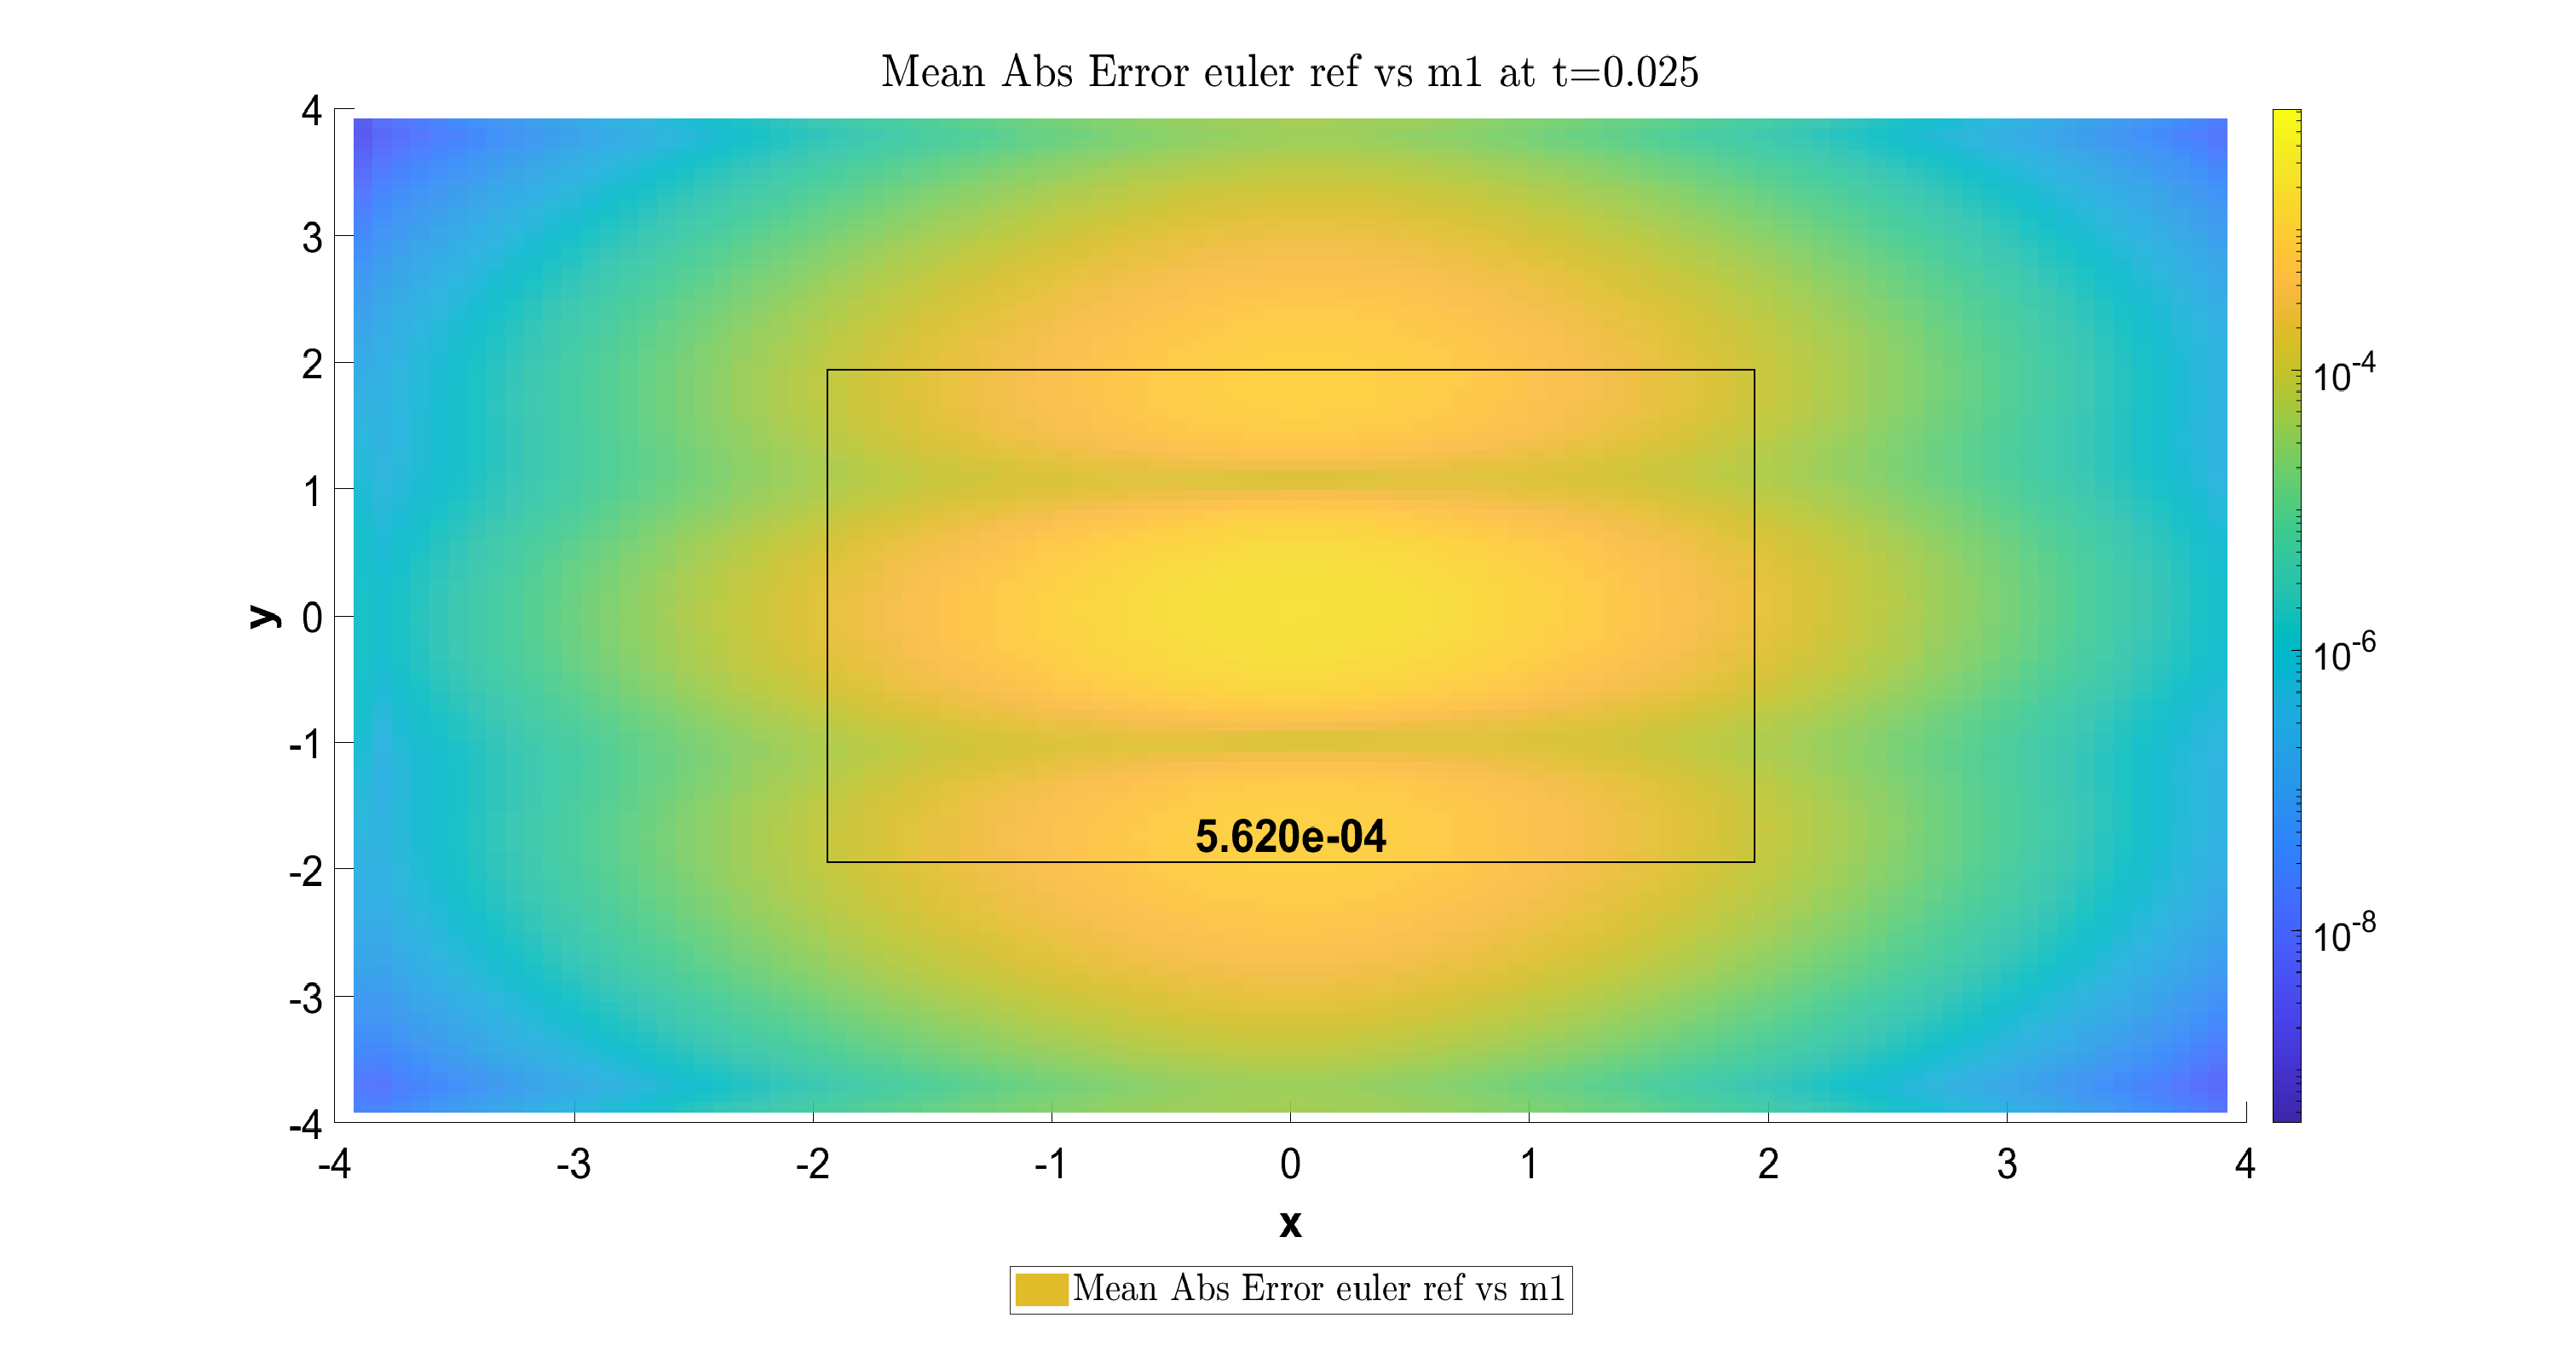
\includegraphics[width=.95\columnwidth]{CDF/CDFEulerRef_1}
\end{landscape}
\begin{landscape}
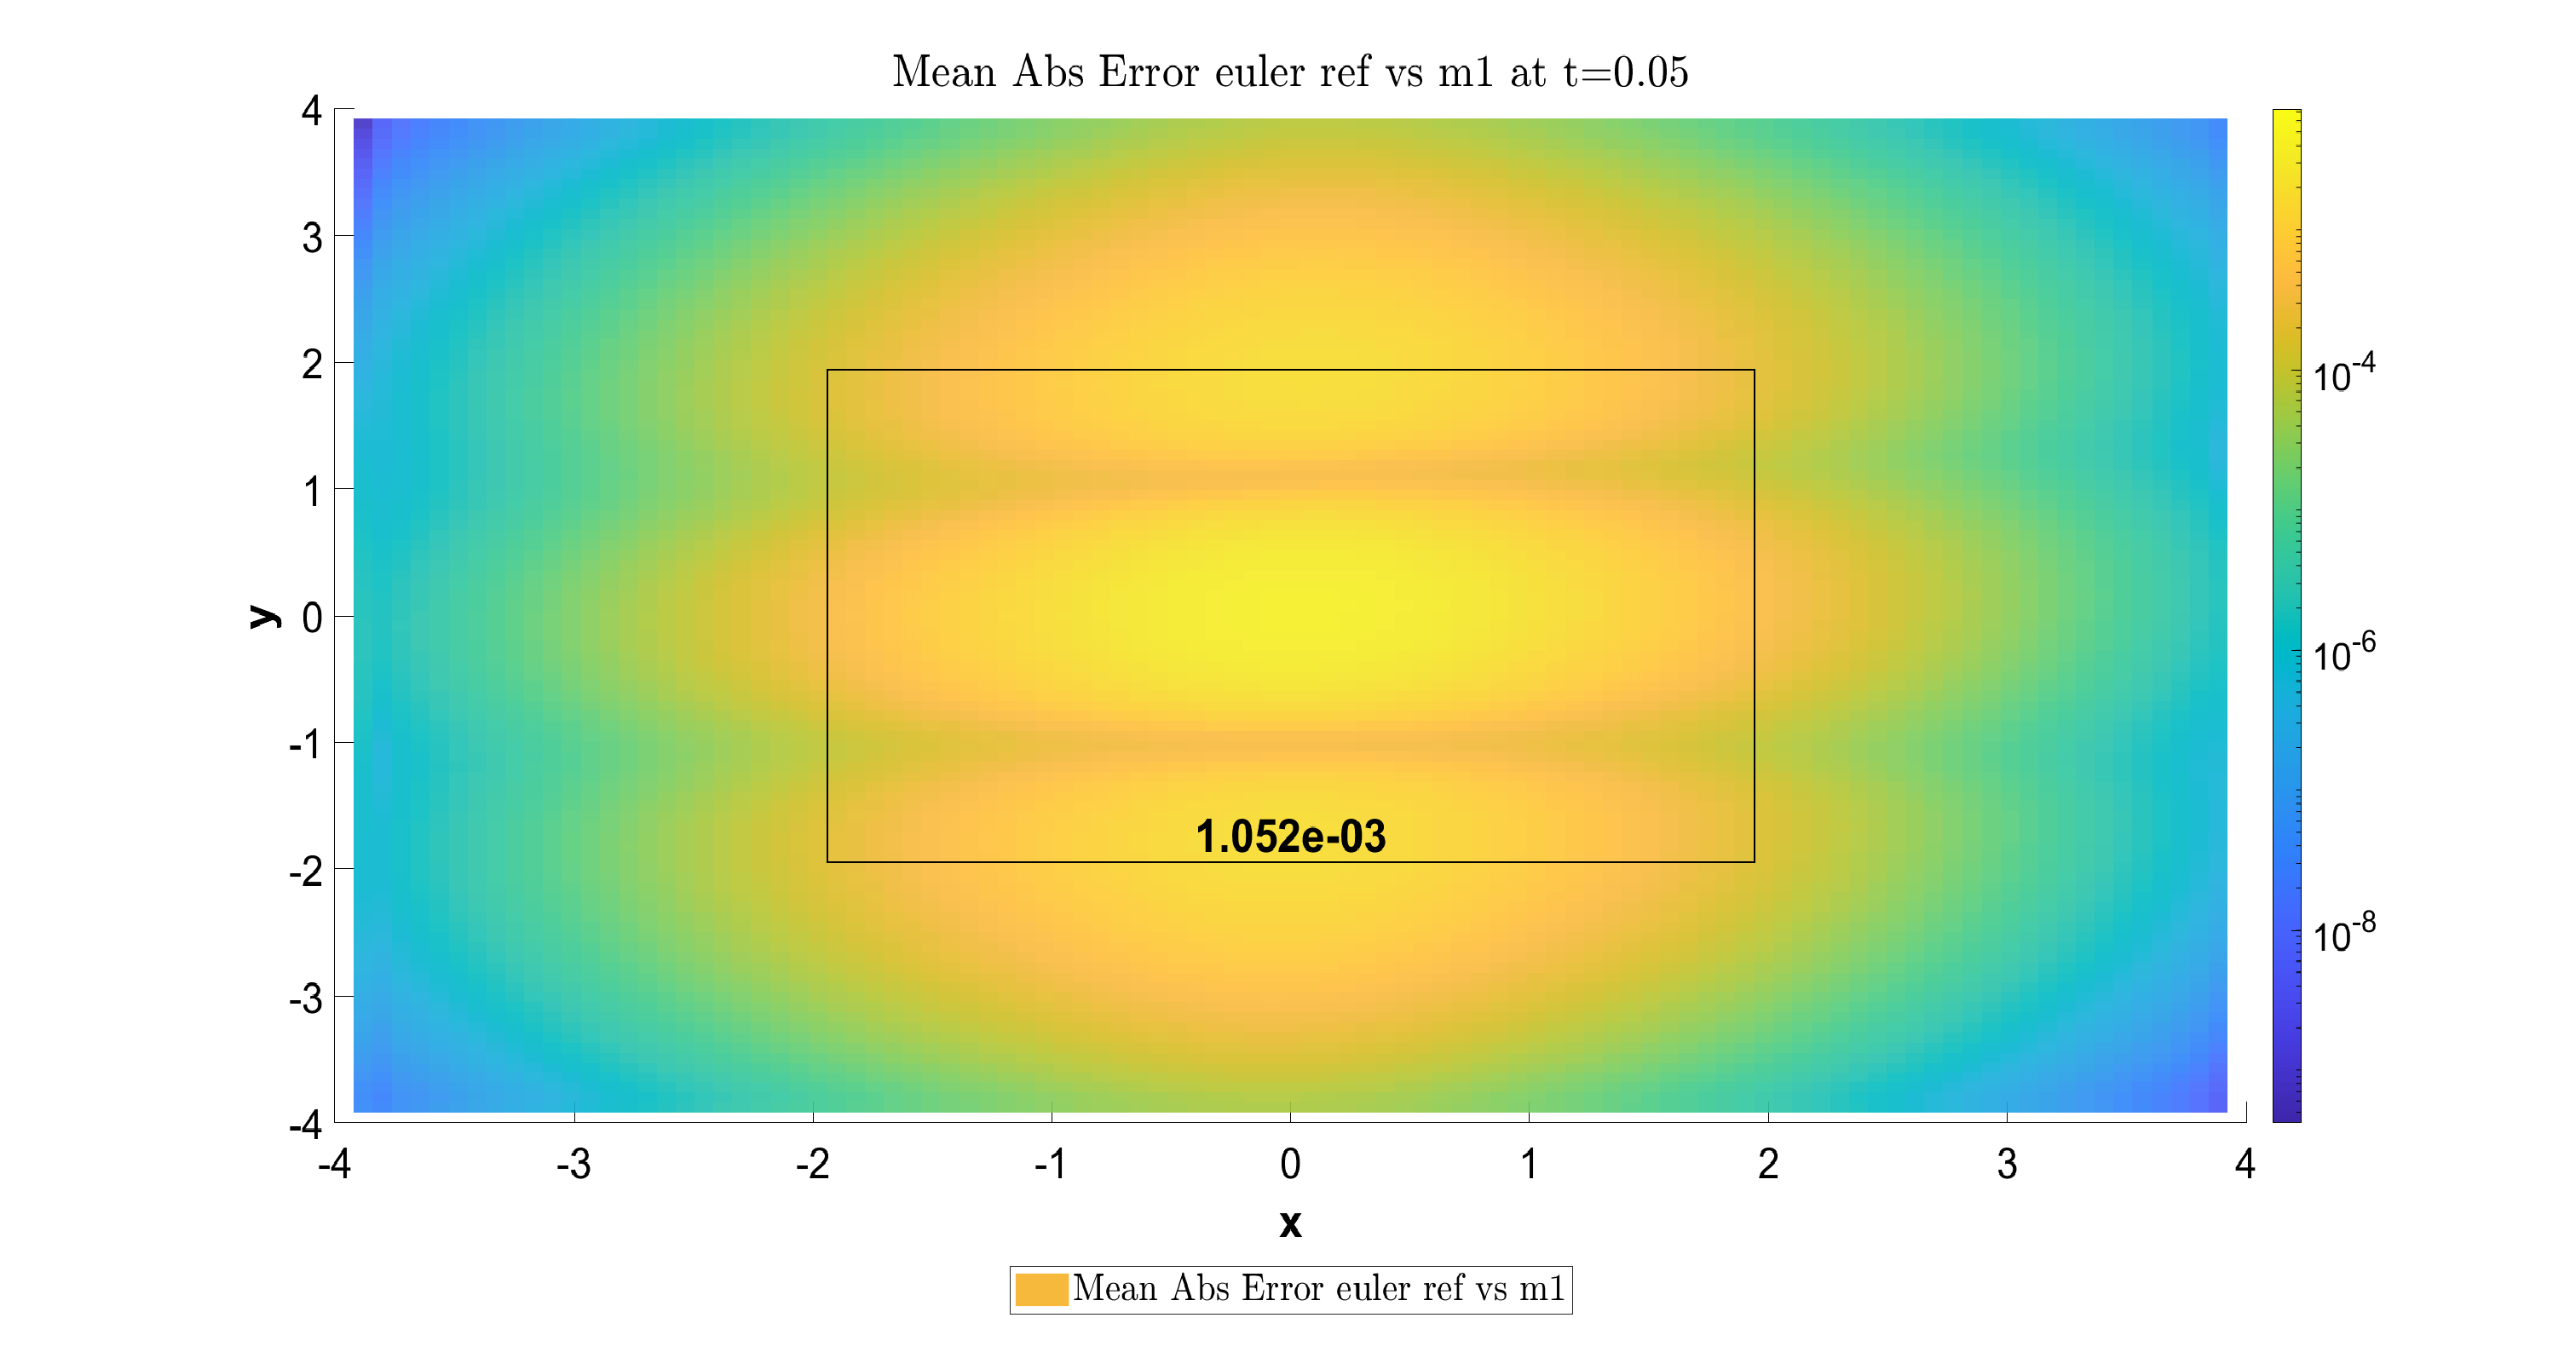
\includegraphics[width=.95\columnwidth]{CDF/CDFEulerRef_2}
\end{landscape}
\begin{landscape}
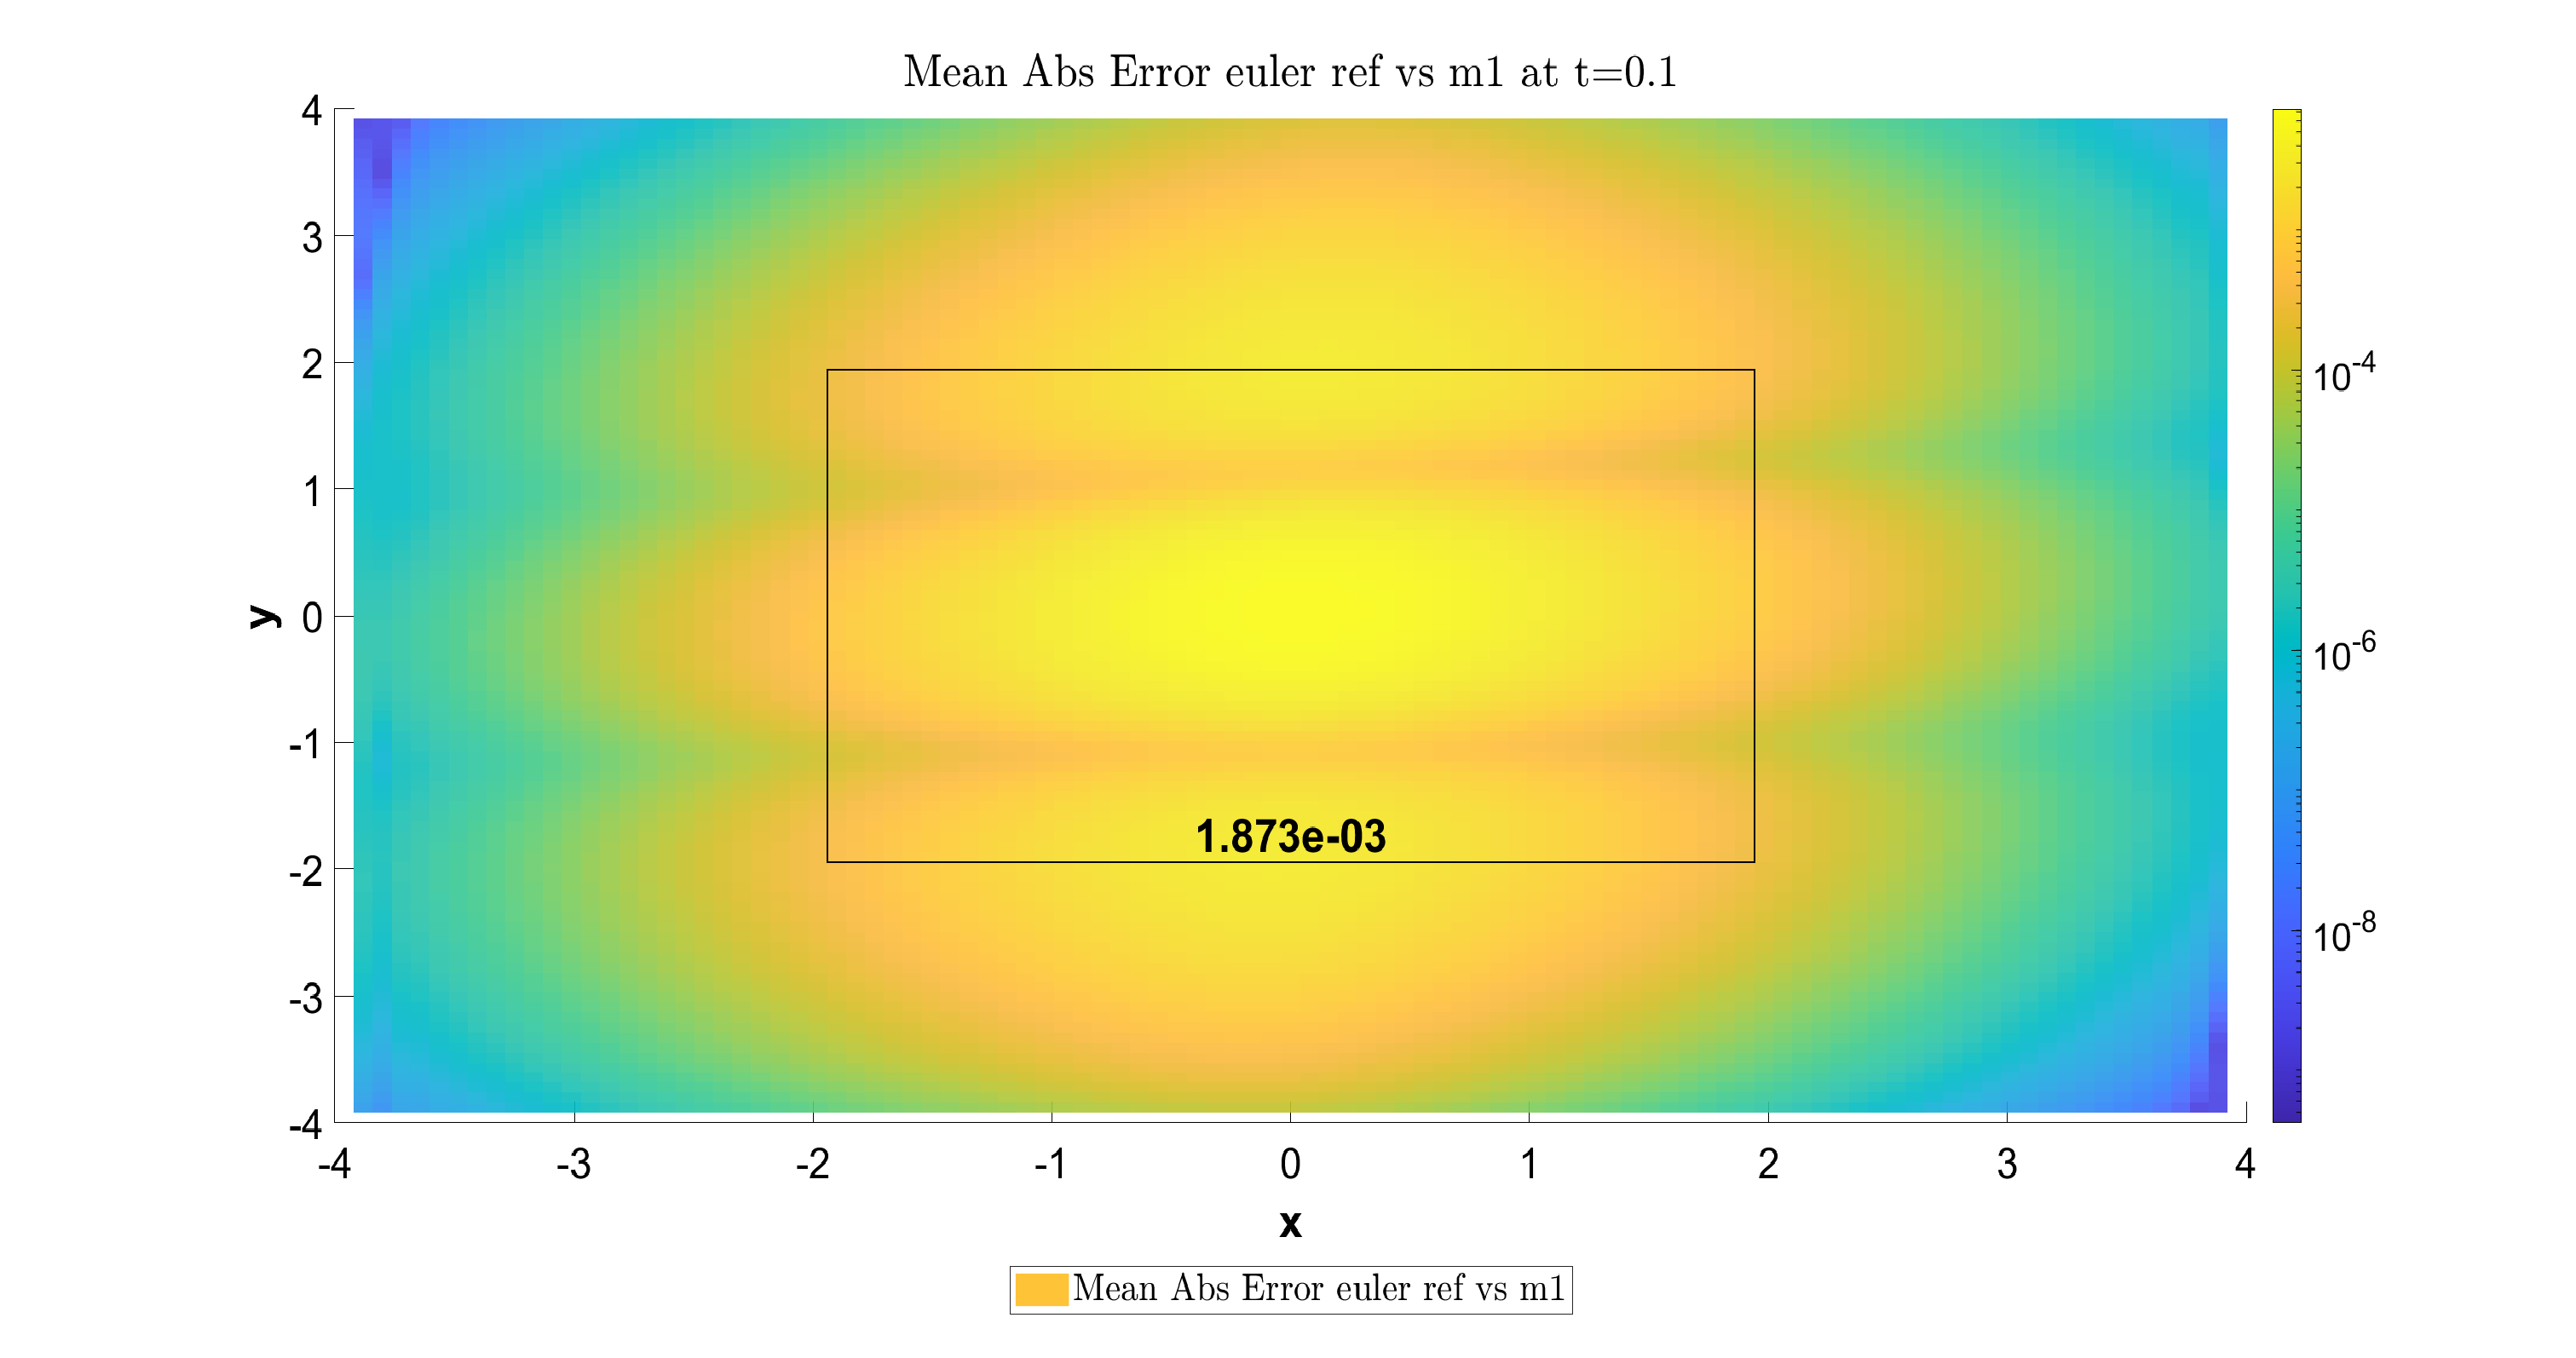
\includegraphics[width=.95\columnwidth]{CDF/CDFEulerRef_3}
\end{landscape}
\begin{landscape}
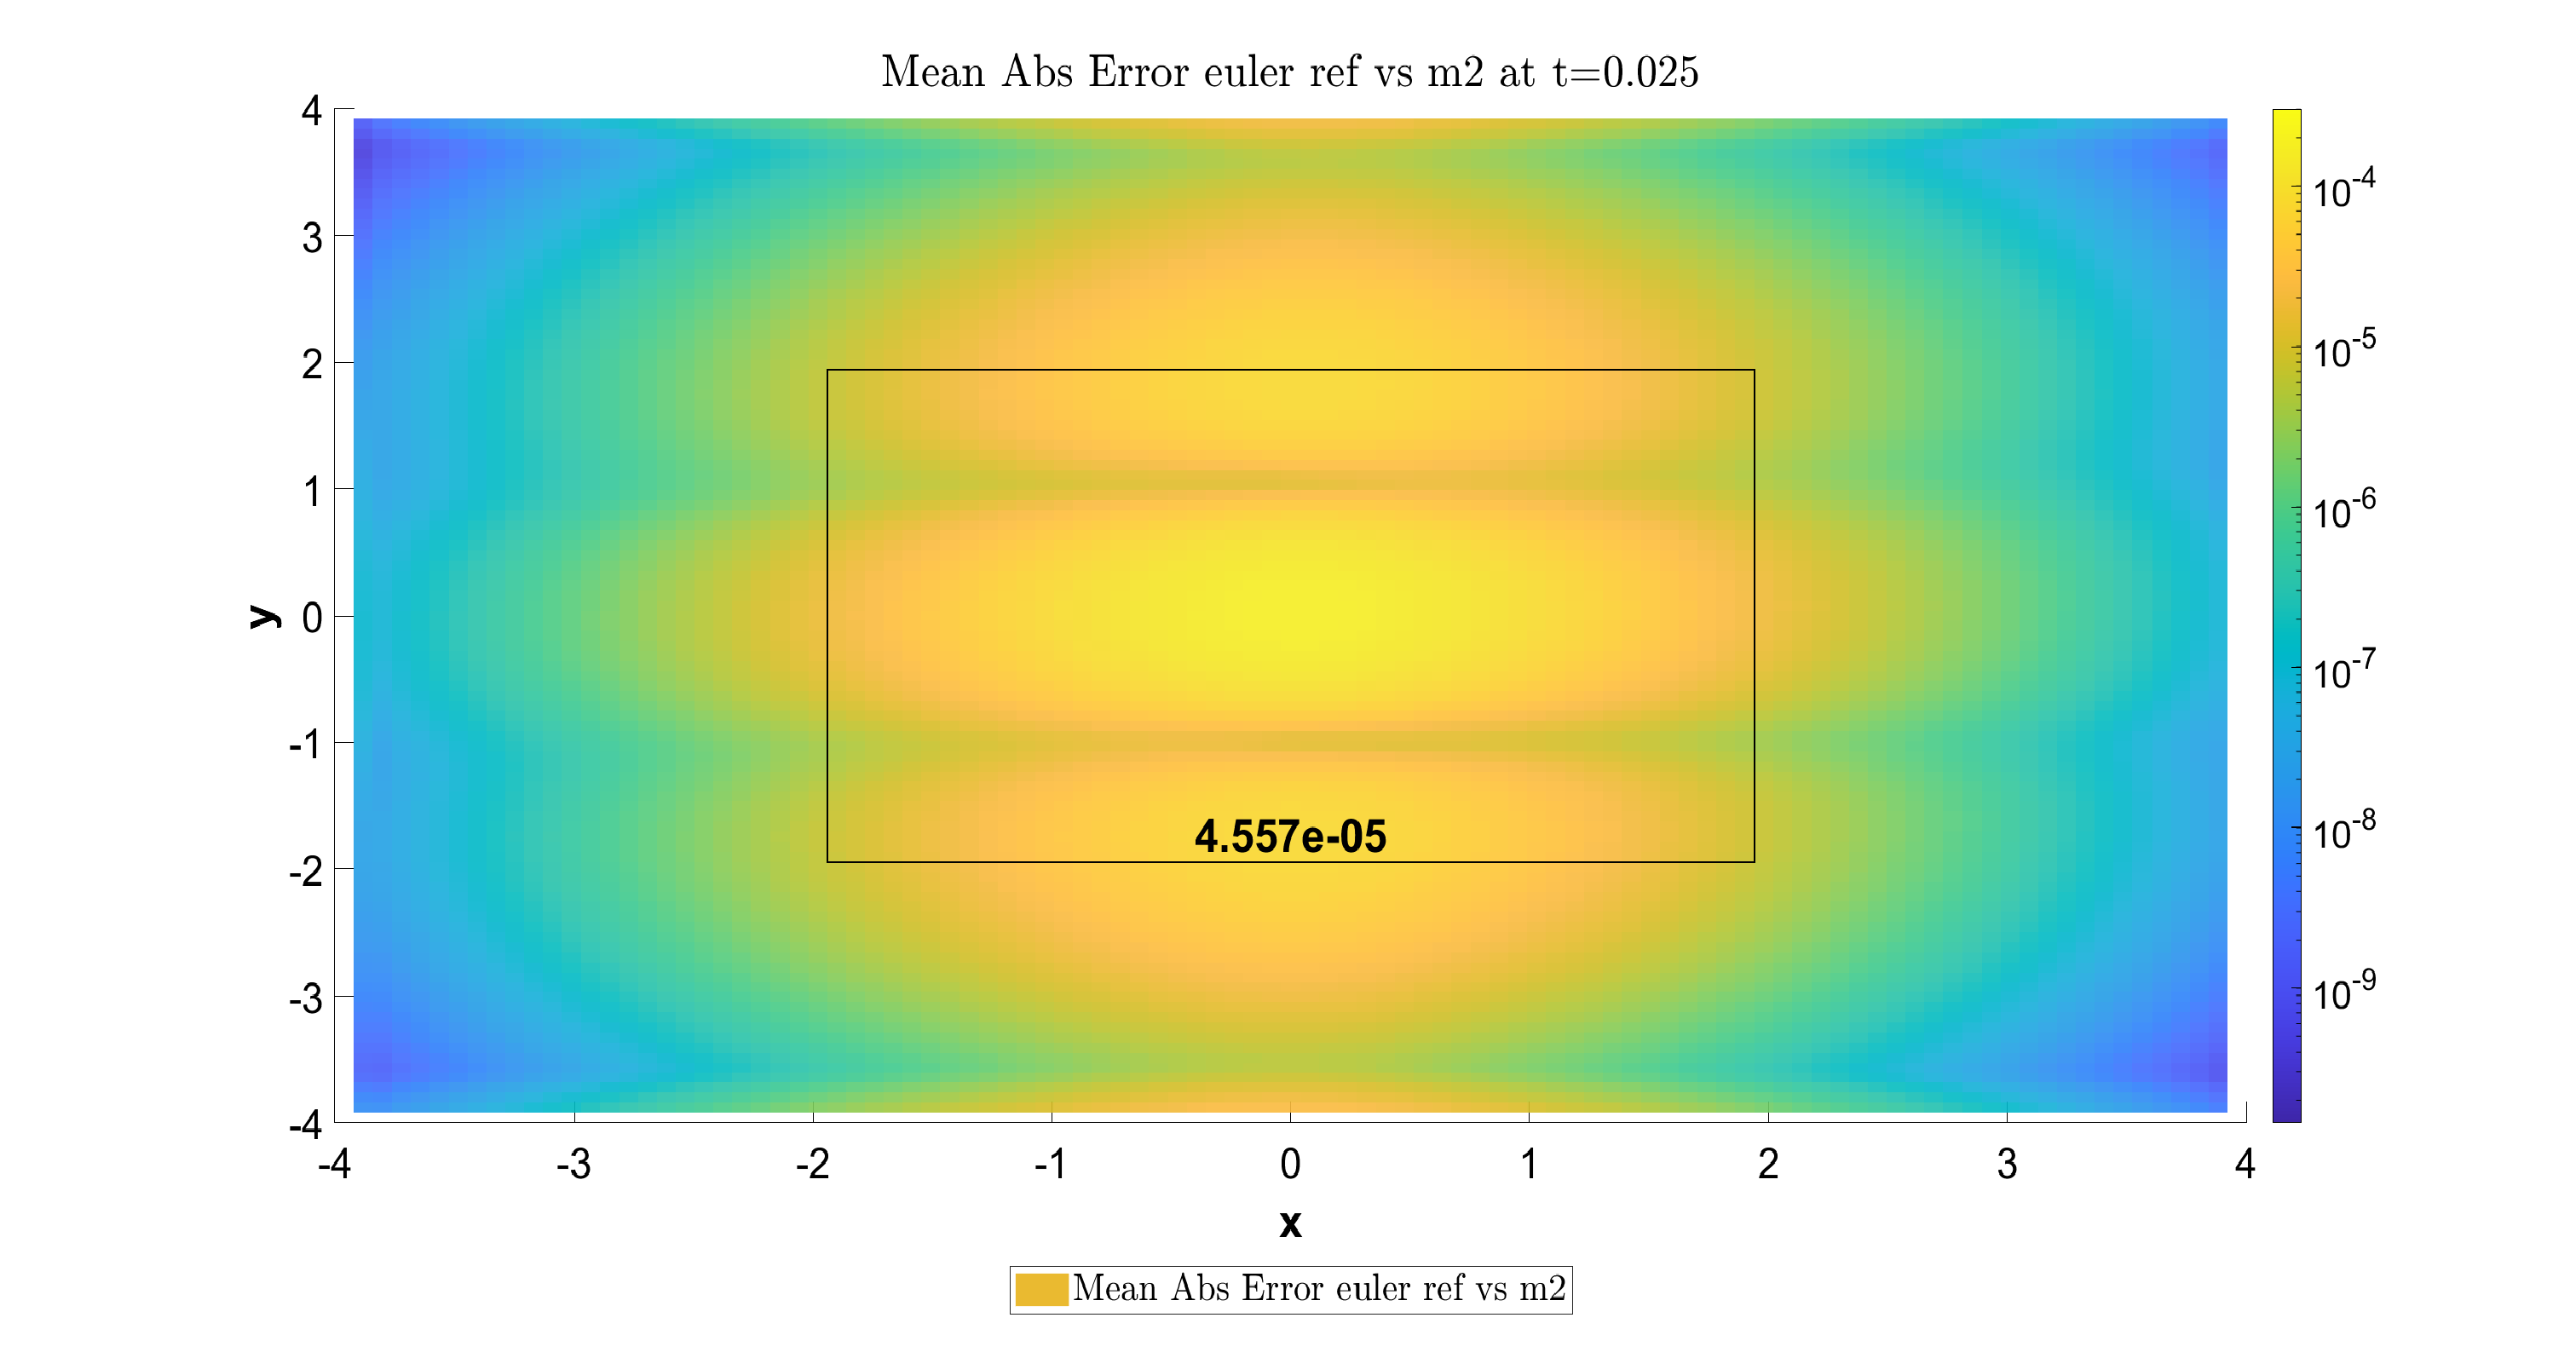
\includegraphics[width=.95\columnwidth]{CDF/CDFEulerRef_4}
\end{landscape}
\begin{landscape}
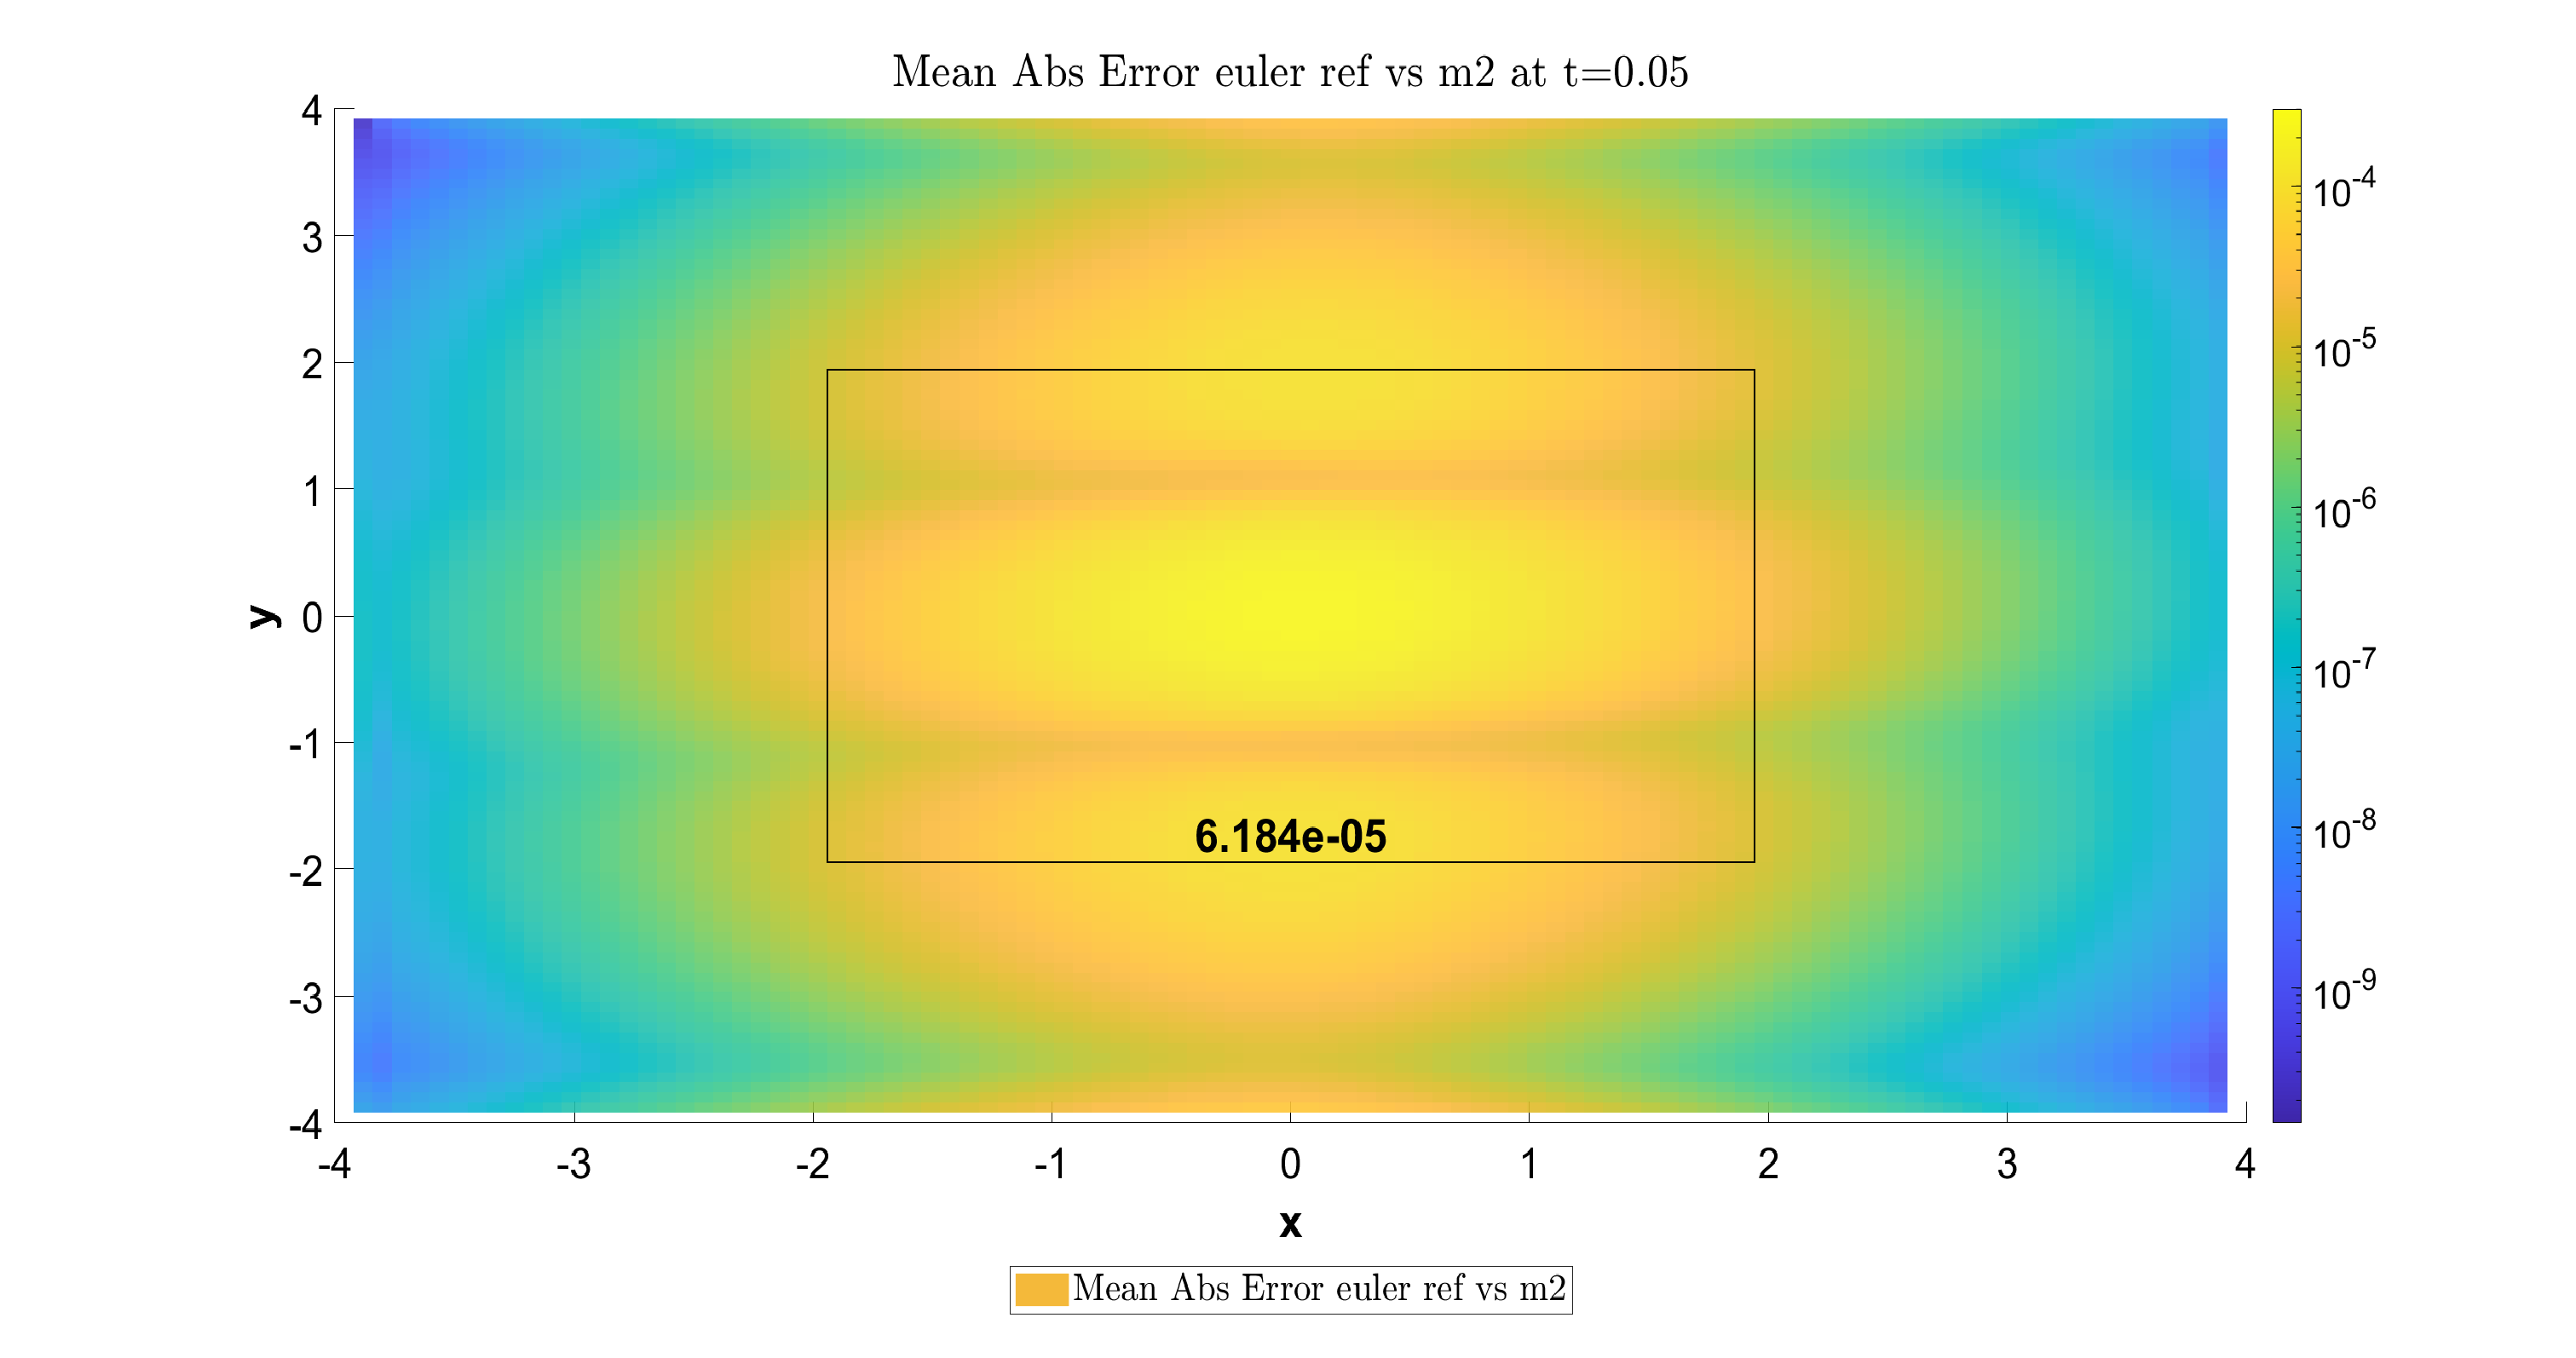
\includegraphics[width=.95\columnwidth]{CDF/CDFEulerRef_5}
\end{landscape}
\begin{landscape}
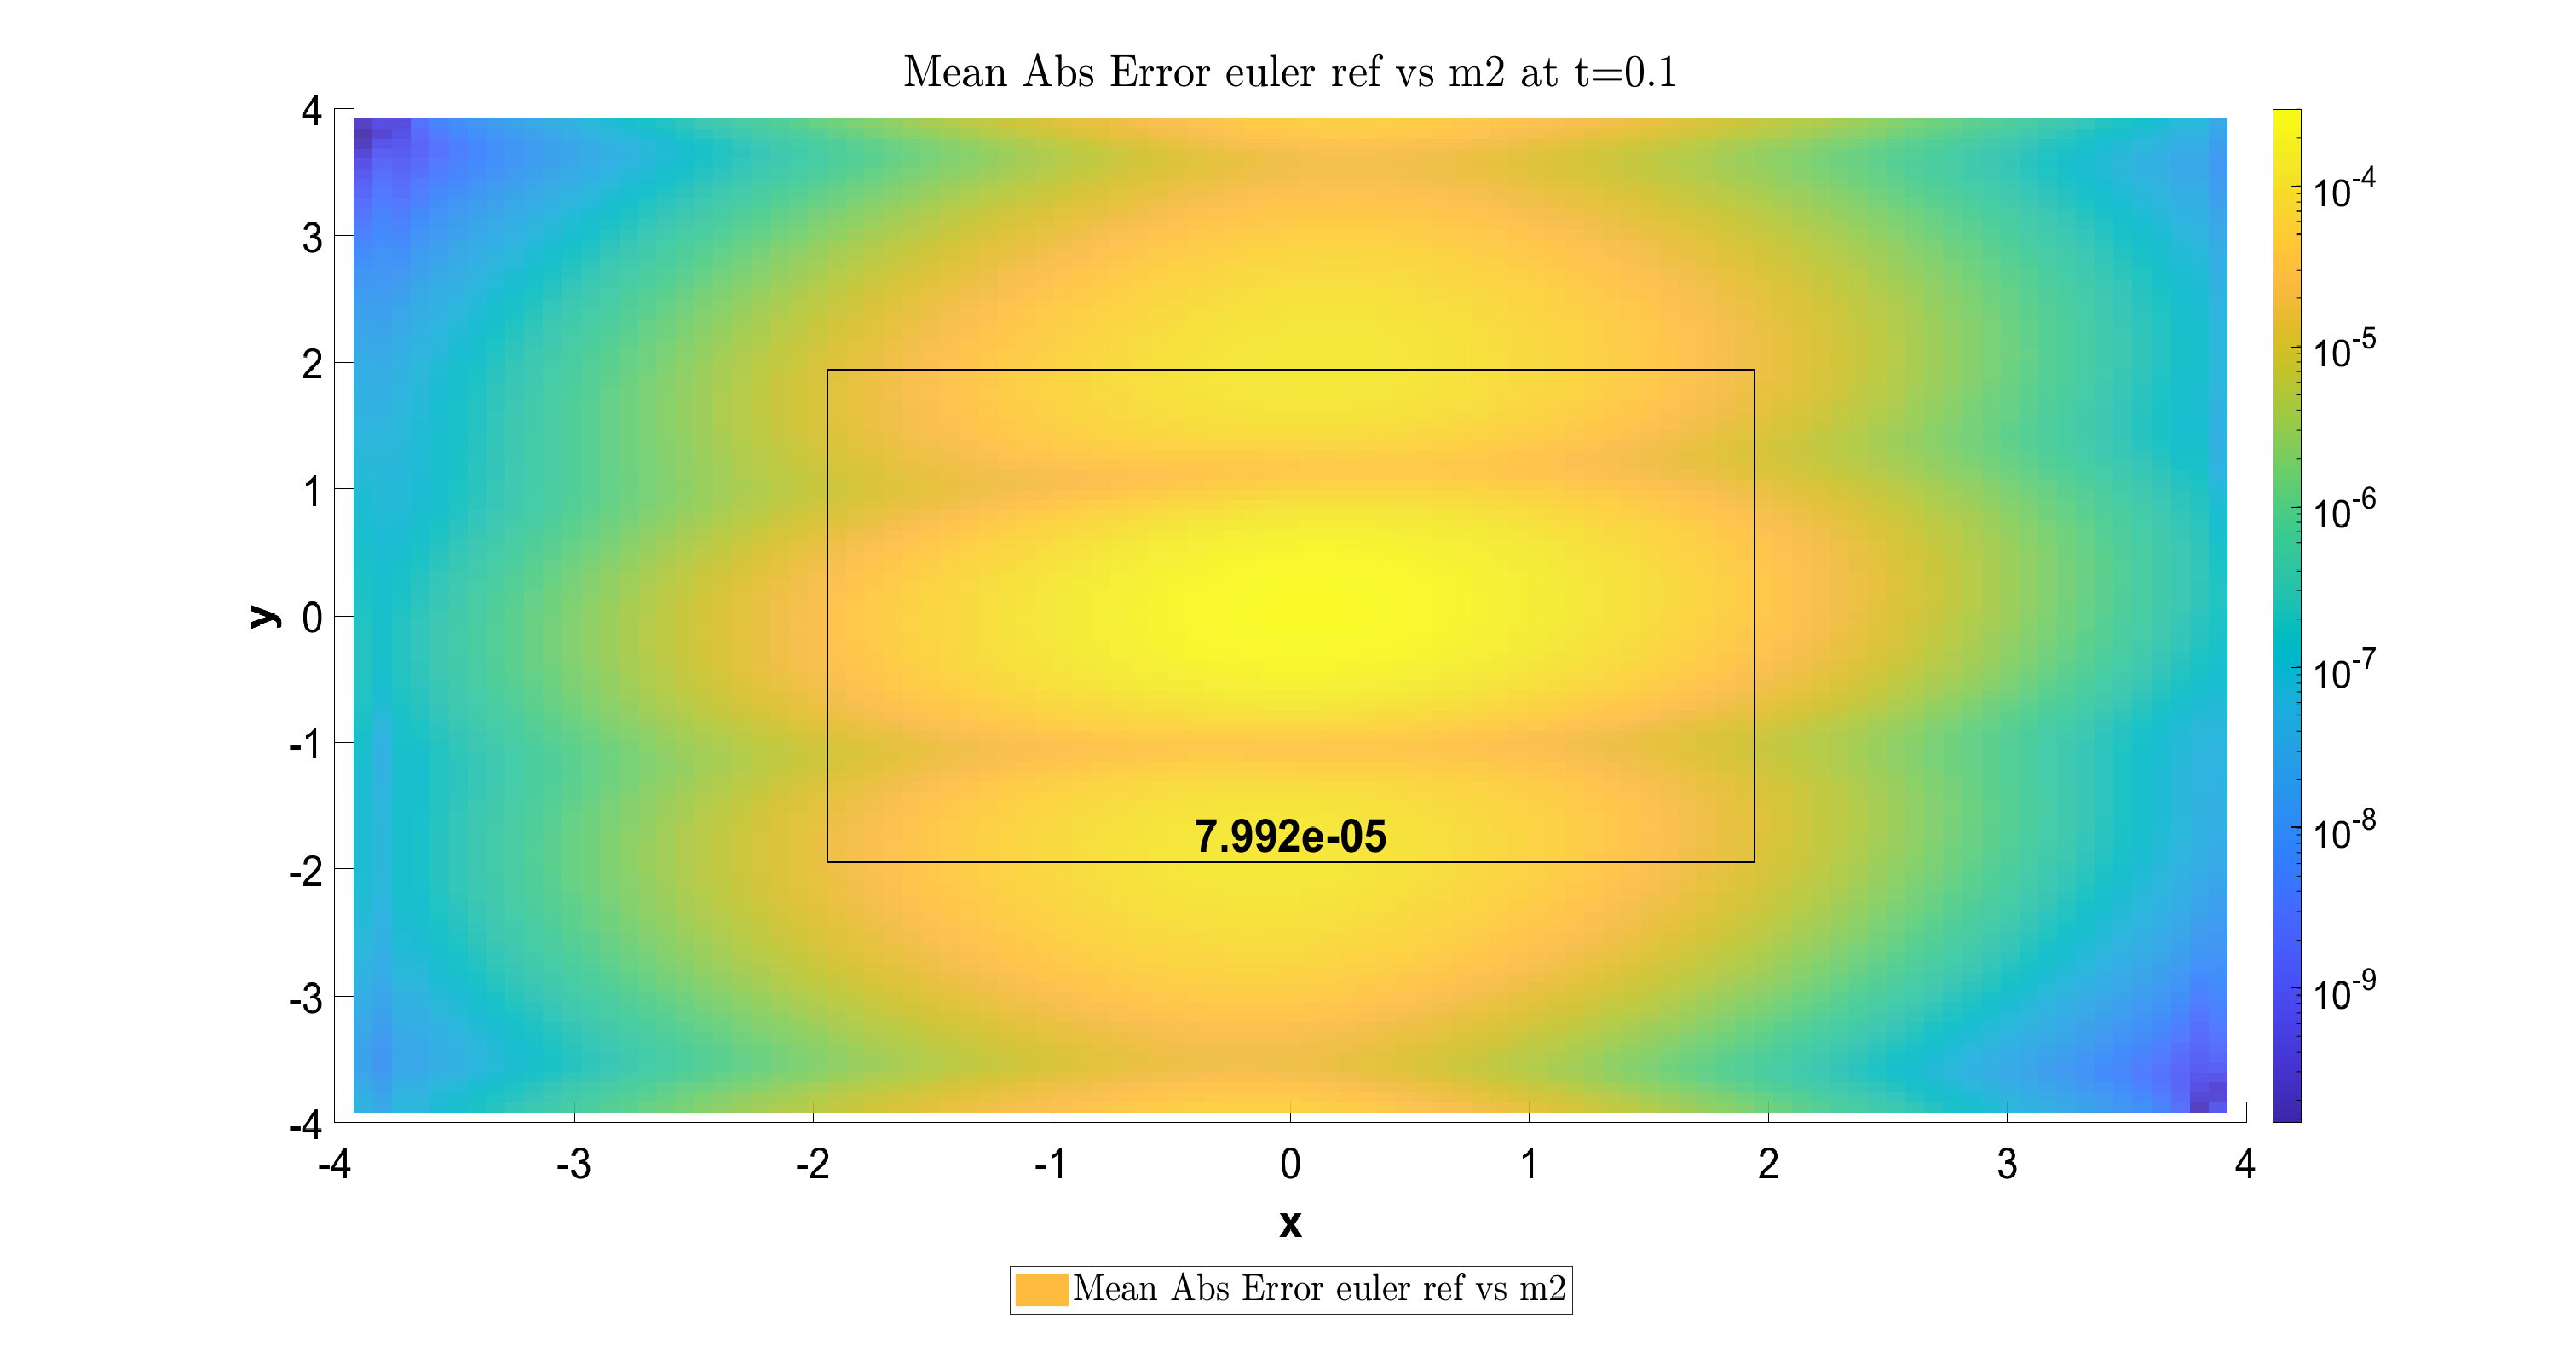
\includegraphics[width=.95\columnwidth]{CDF/CDFEulerRef_6}
\end{landscape}
\begin{landscape}
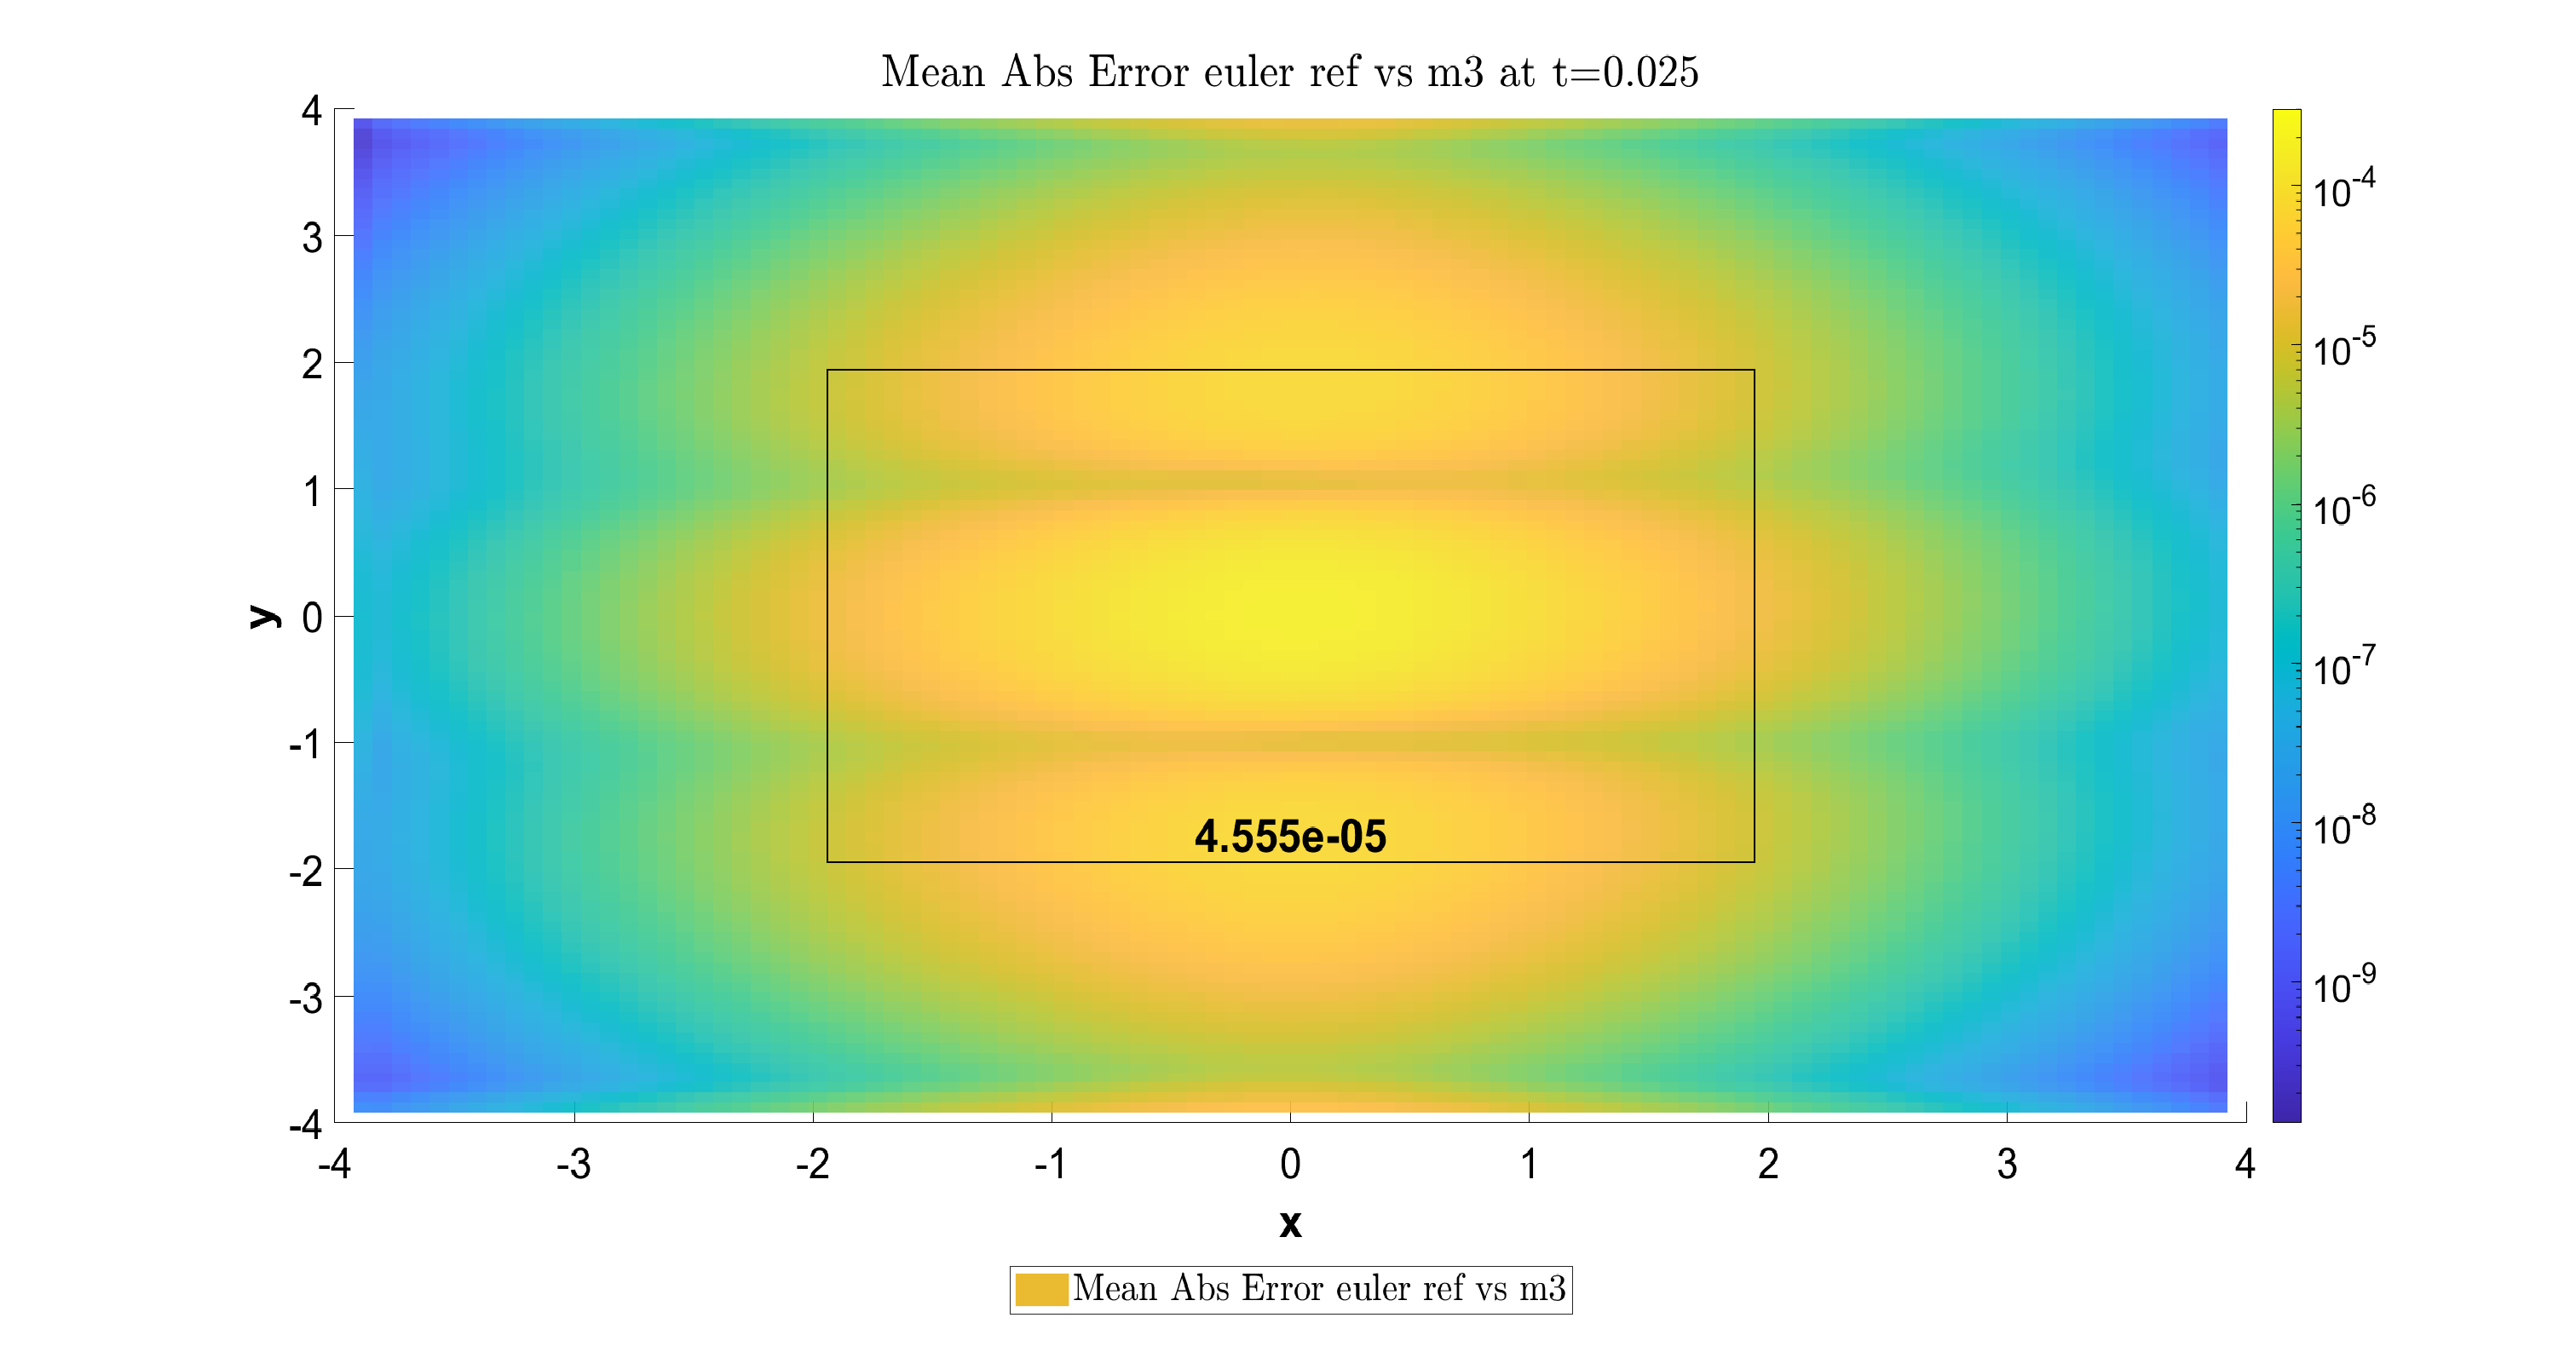
\includegraphics[width=.95\columnwidth]{CDF/CDFEulerRef_7}
\end{landscape}
\begin{landscape}
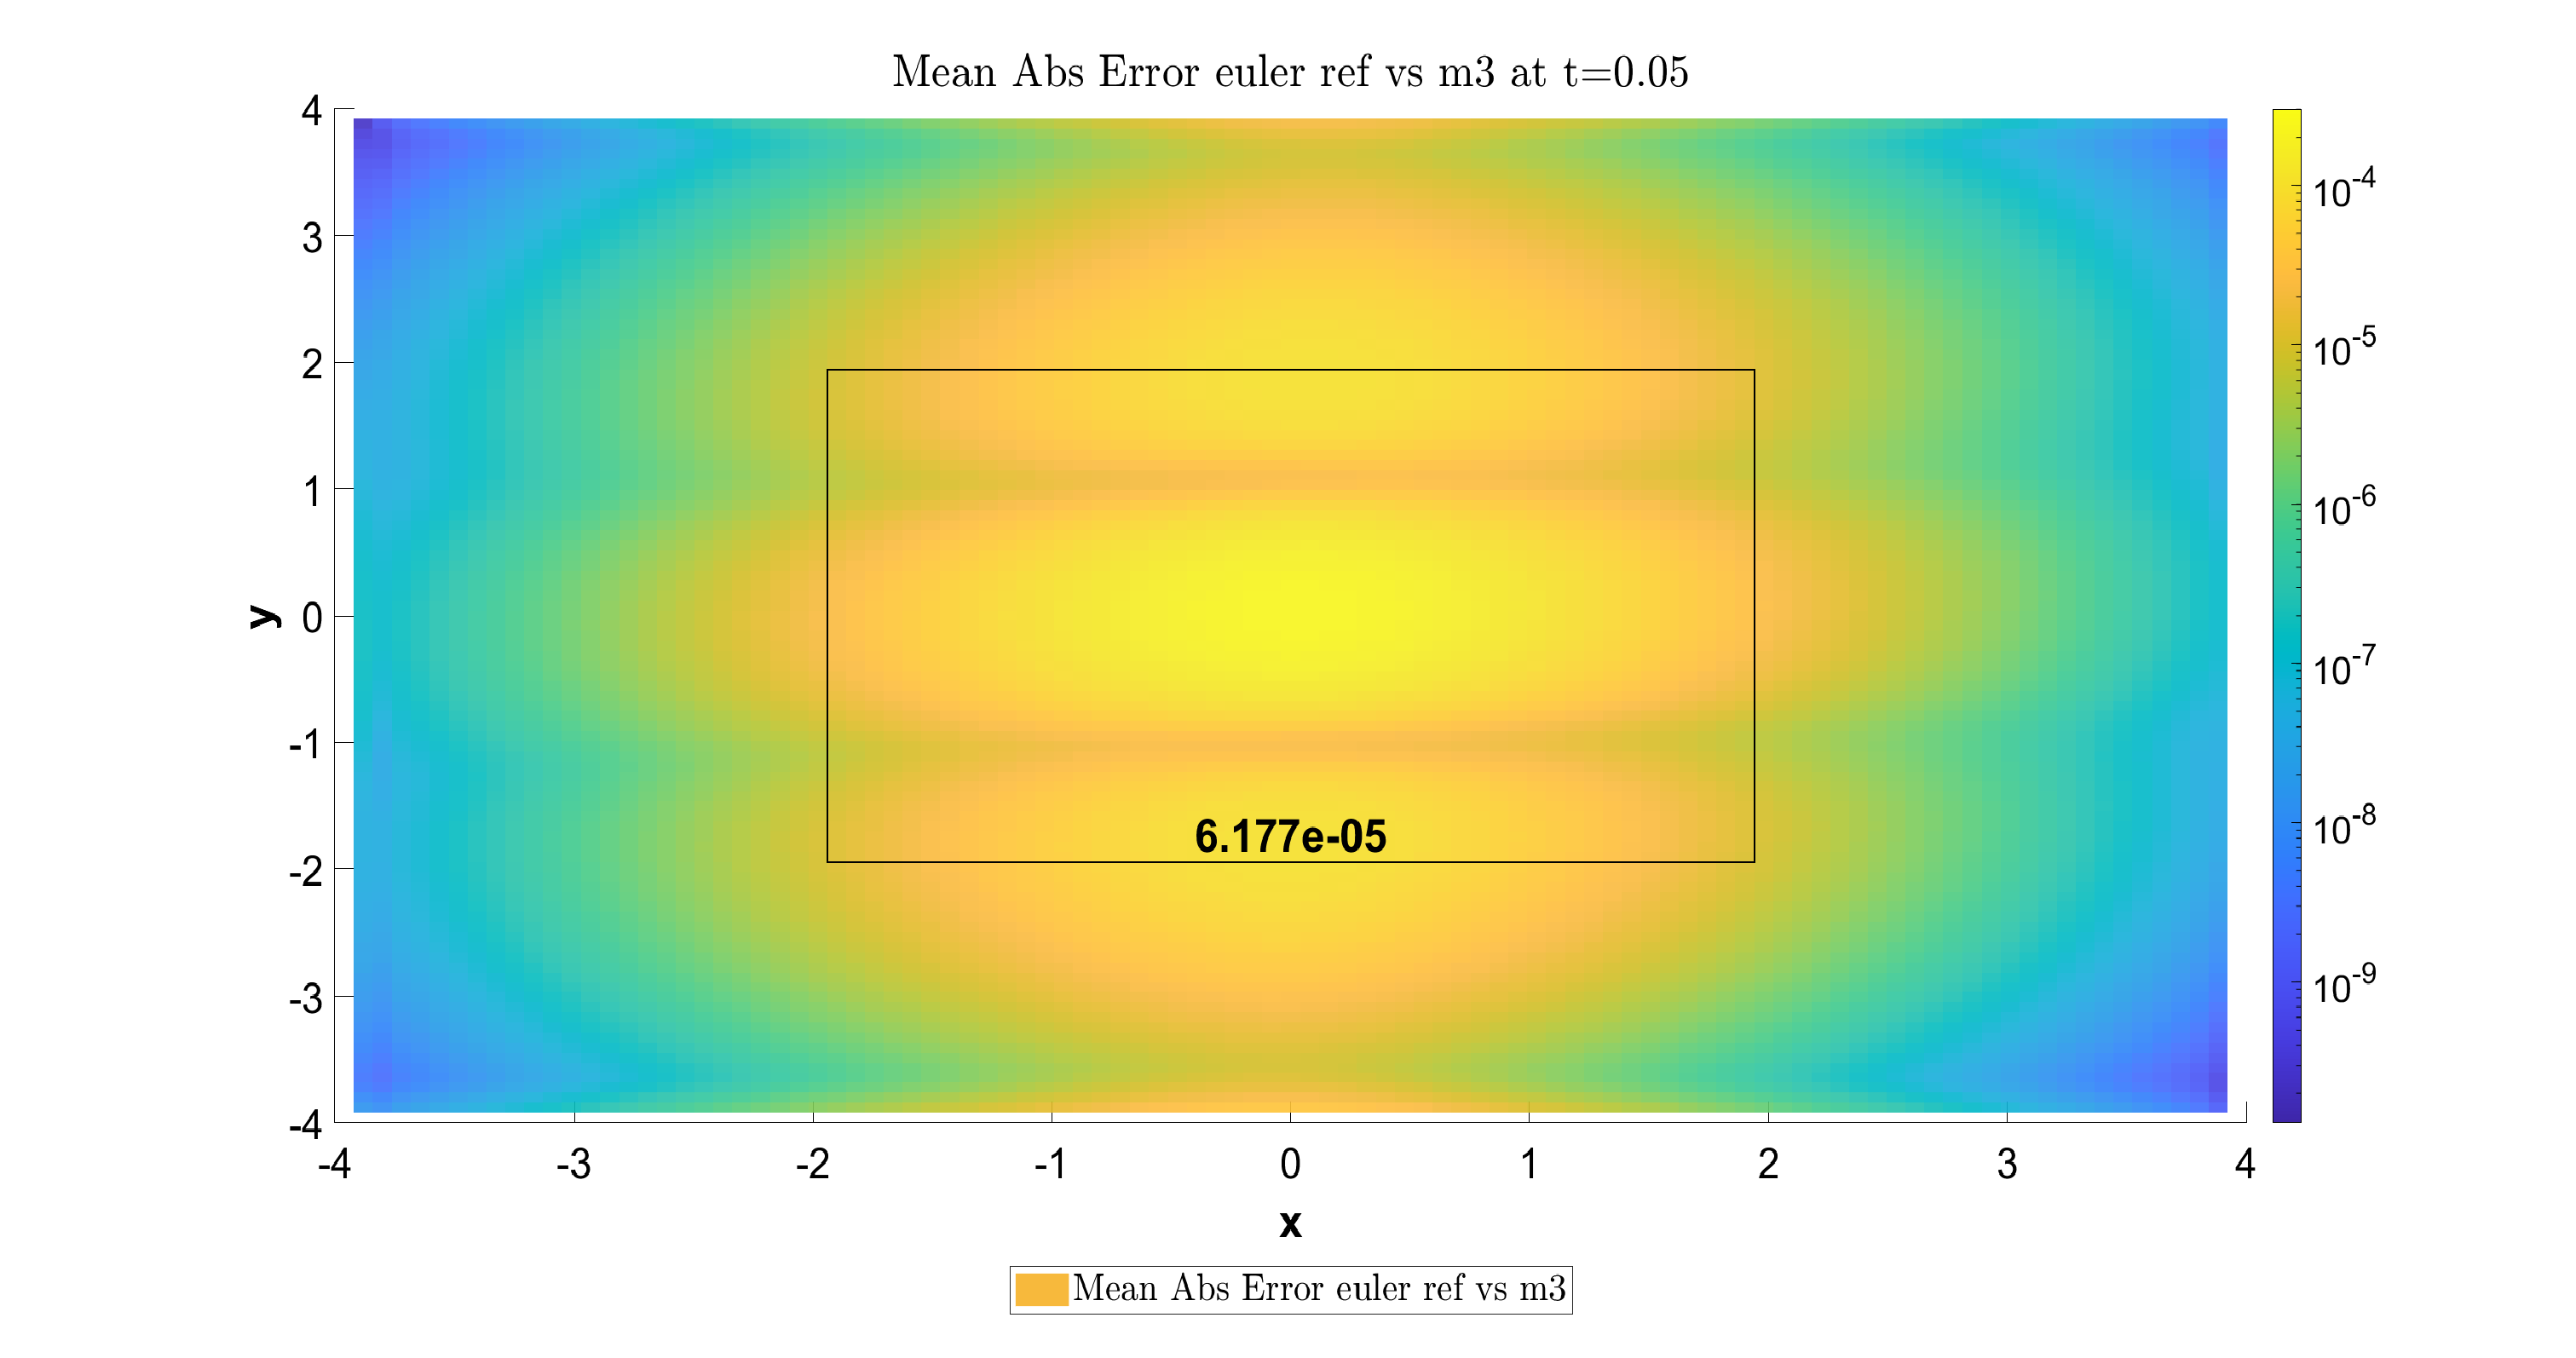
\includegraphics[width=.95\columnwidth]{CDF/CDFEulerRef_8}
\end{landscape}
\begin{landscape}
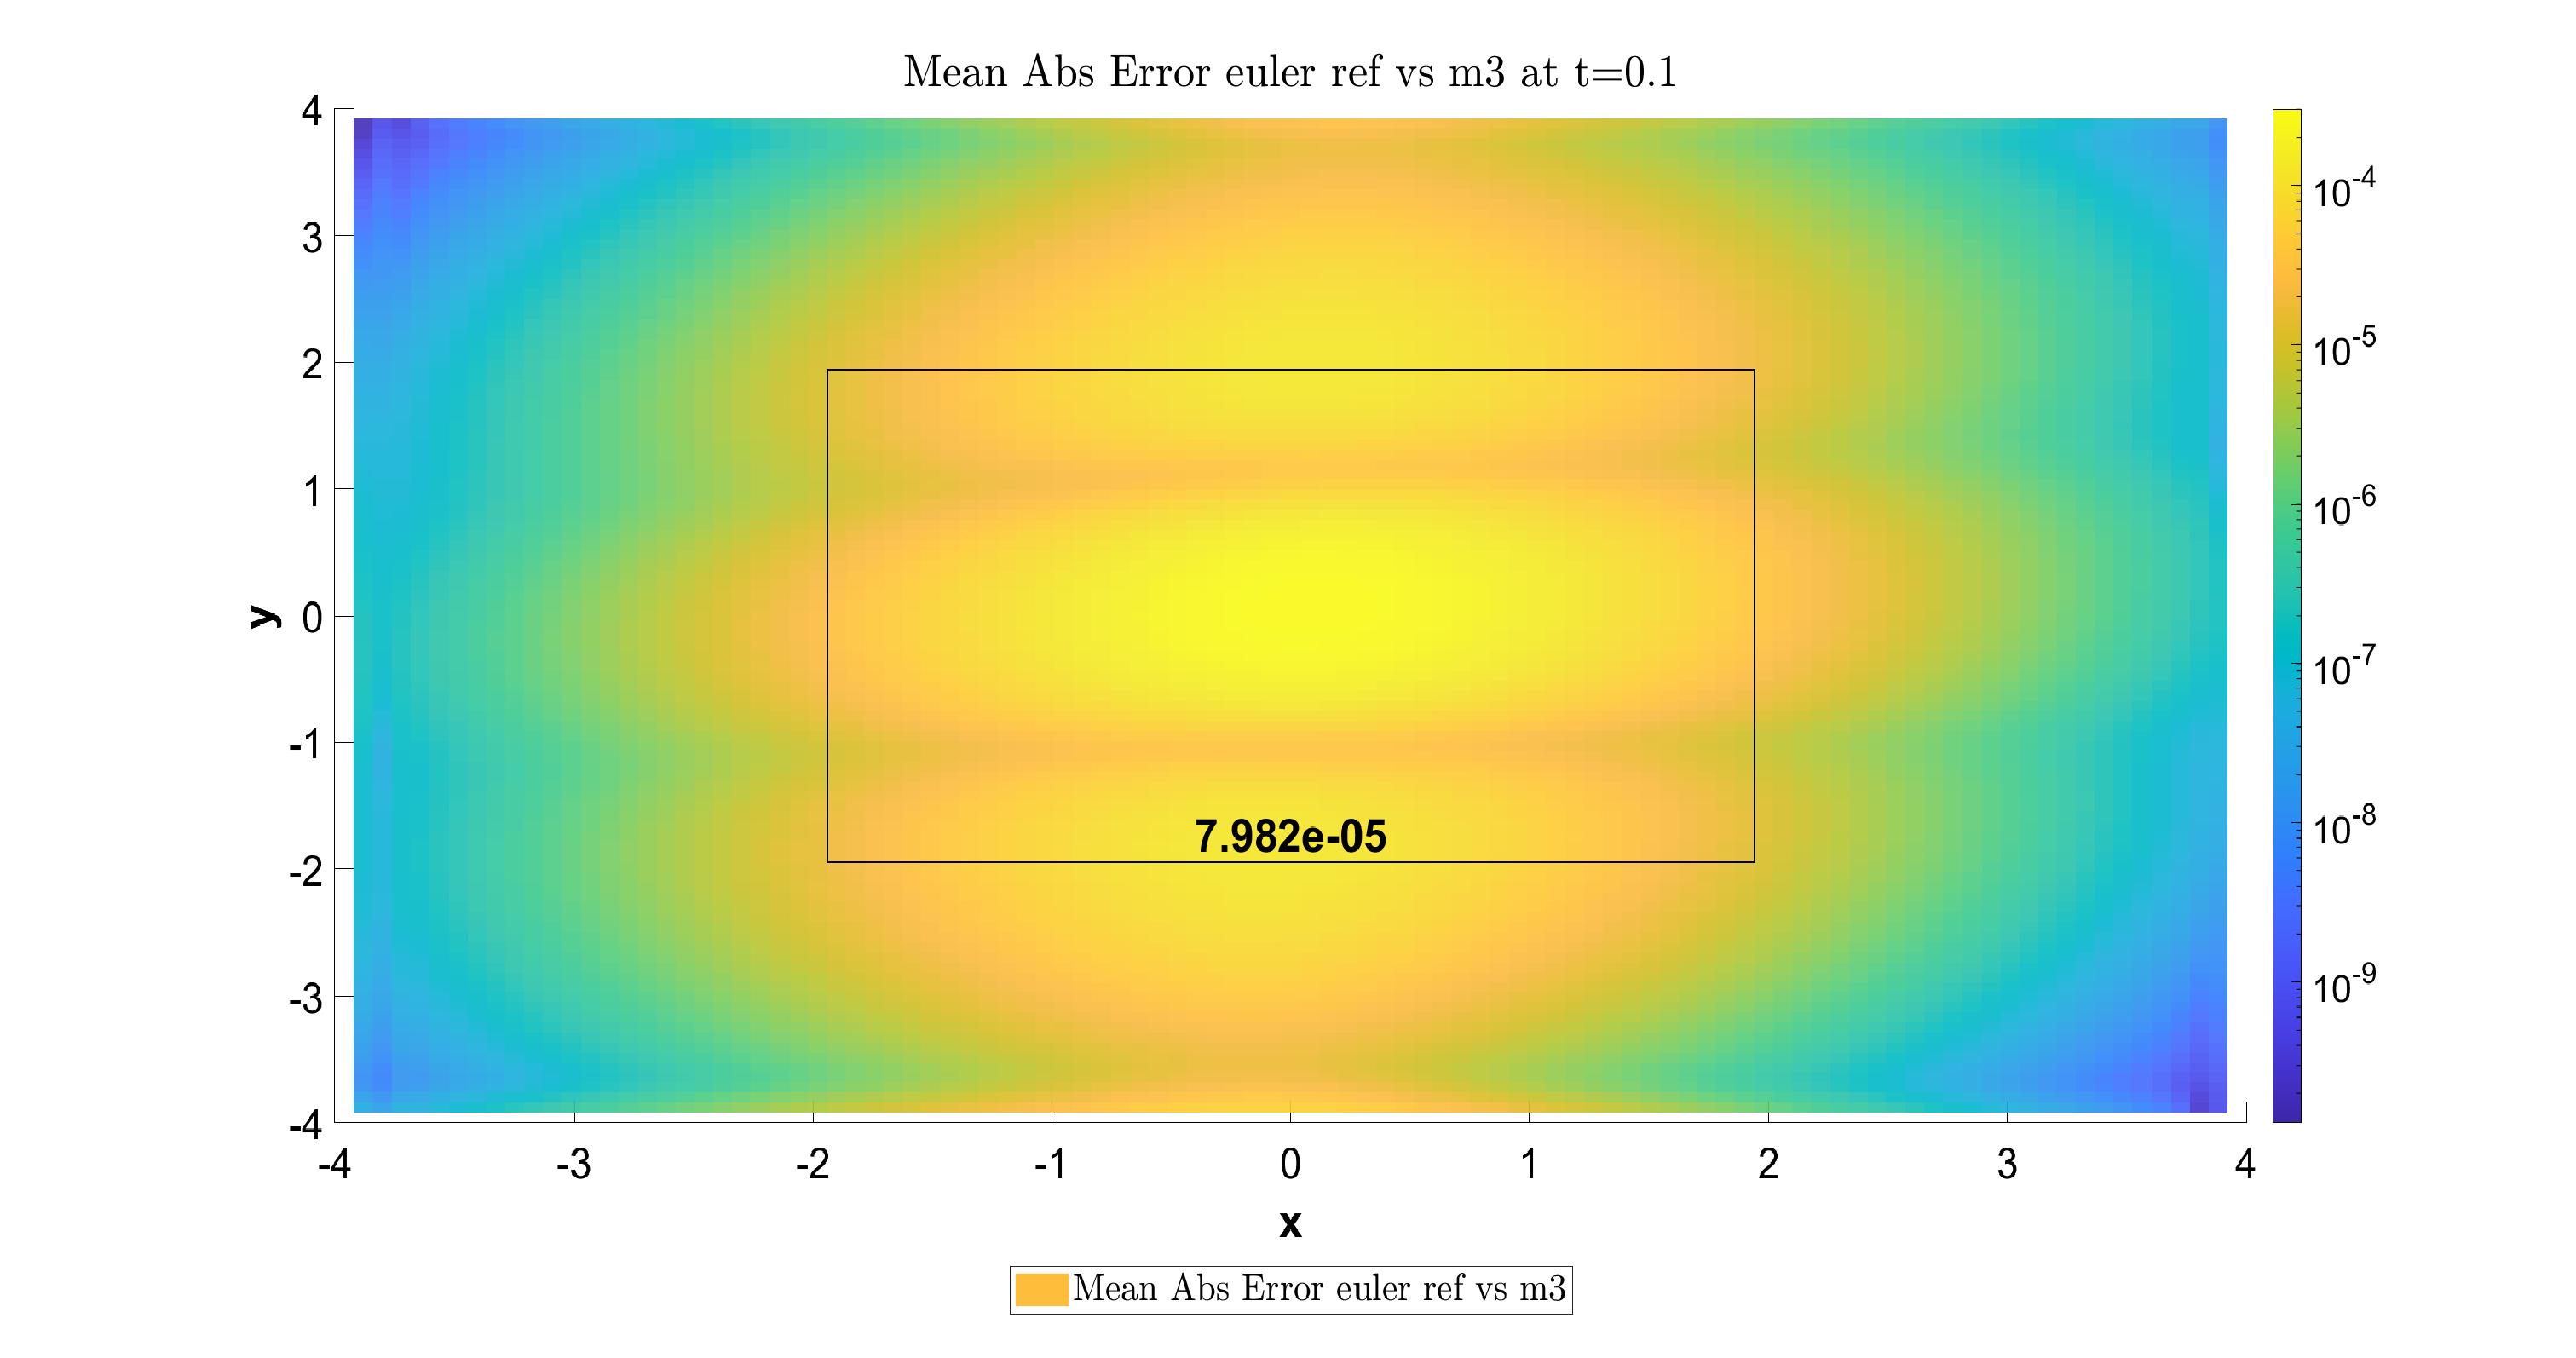
\includegraphics[width=.95\columnwidth]{CDF/CDFEulerRef_9}
\end{landscape}
\begin{landscape}
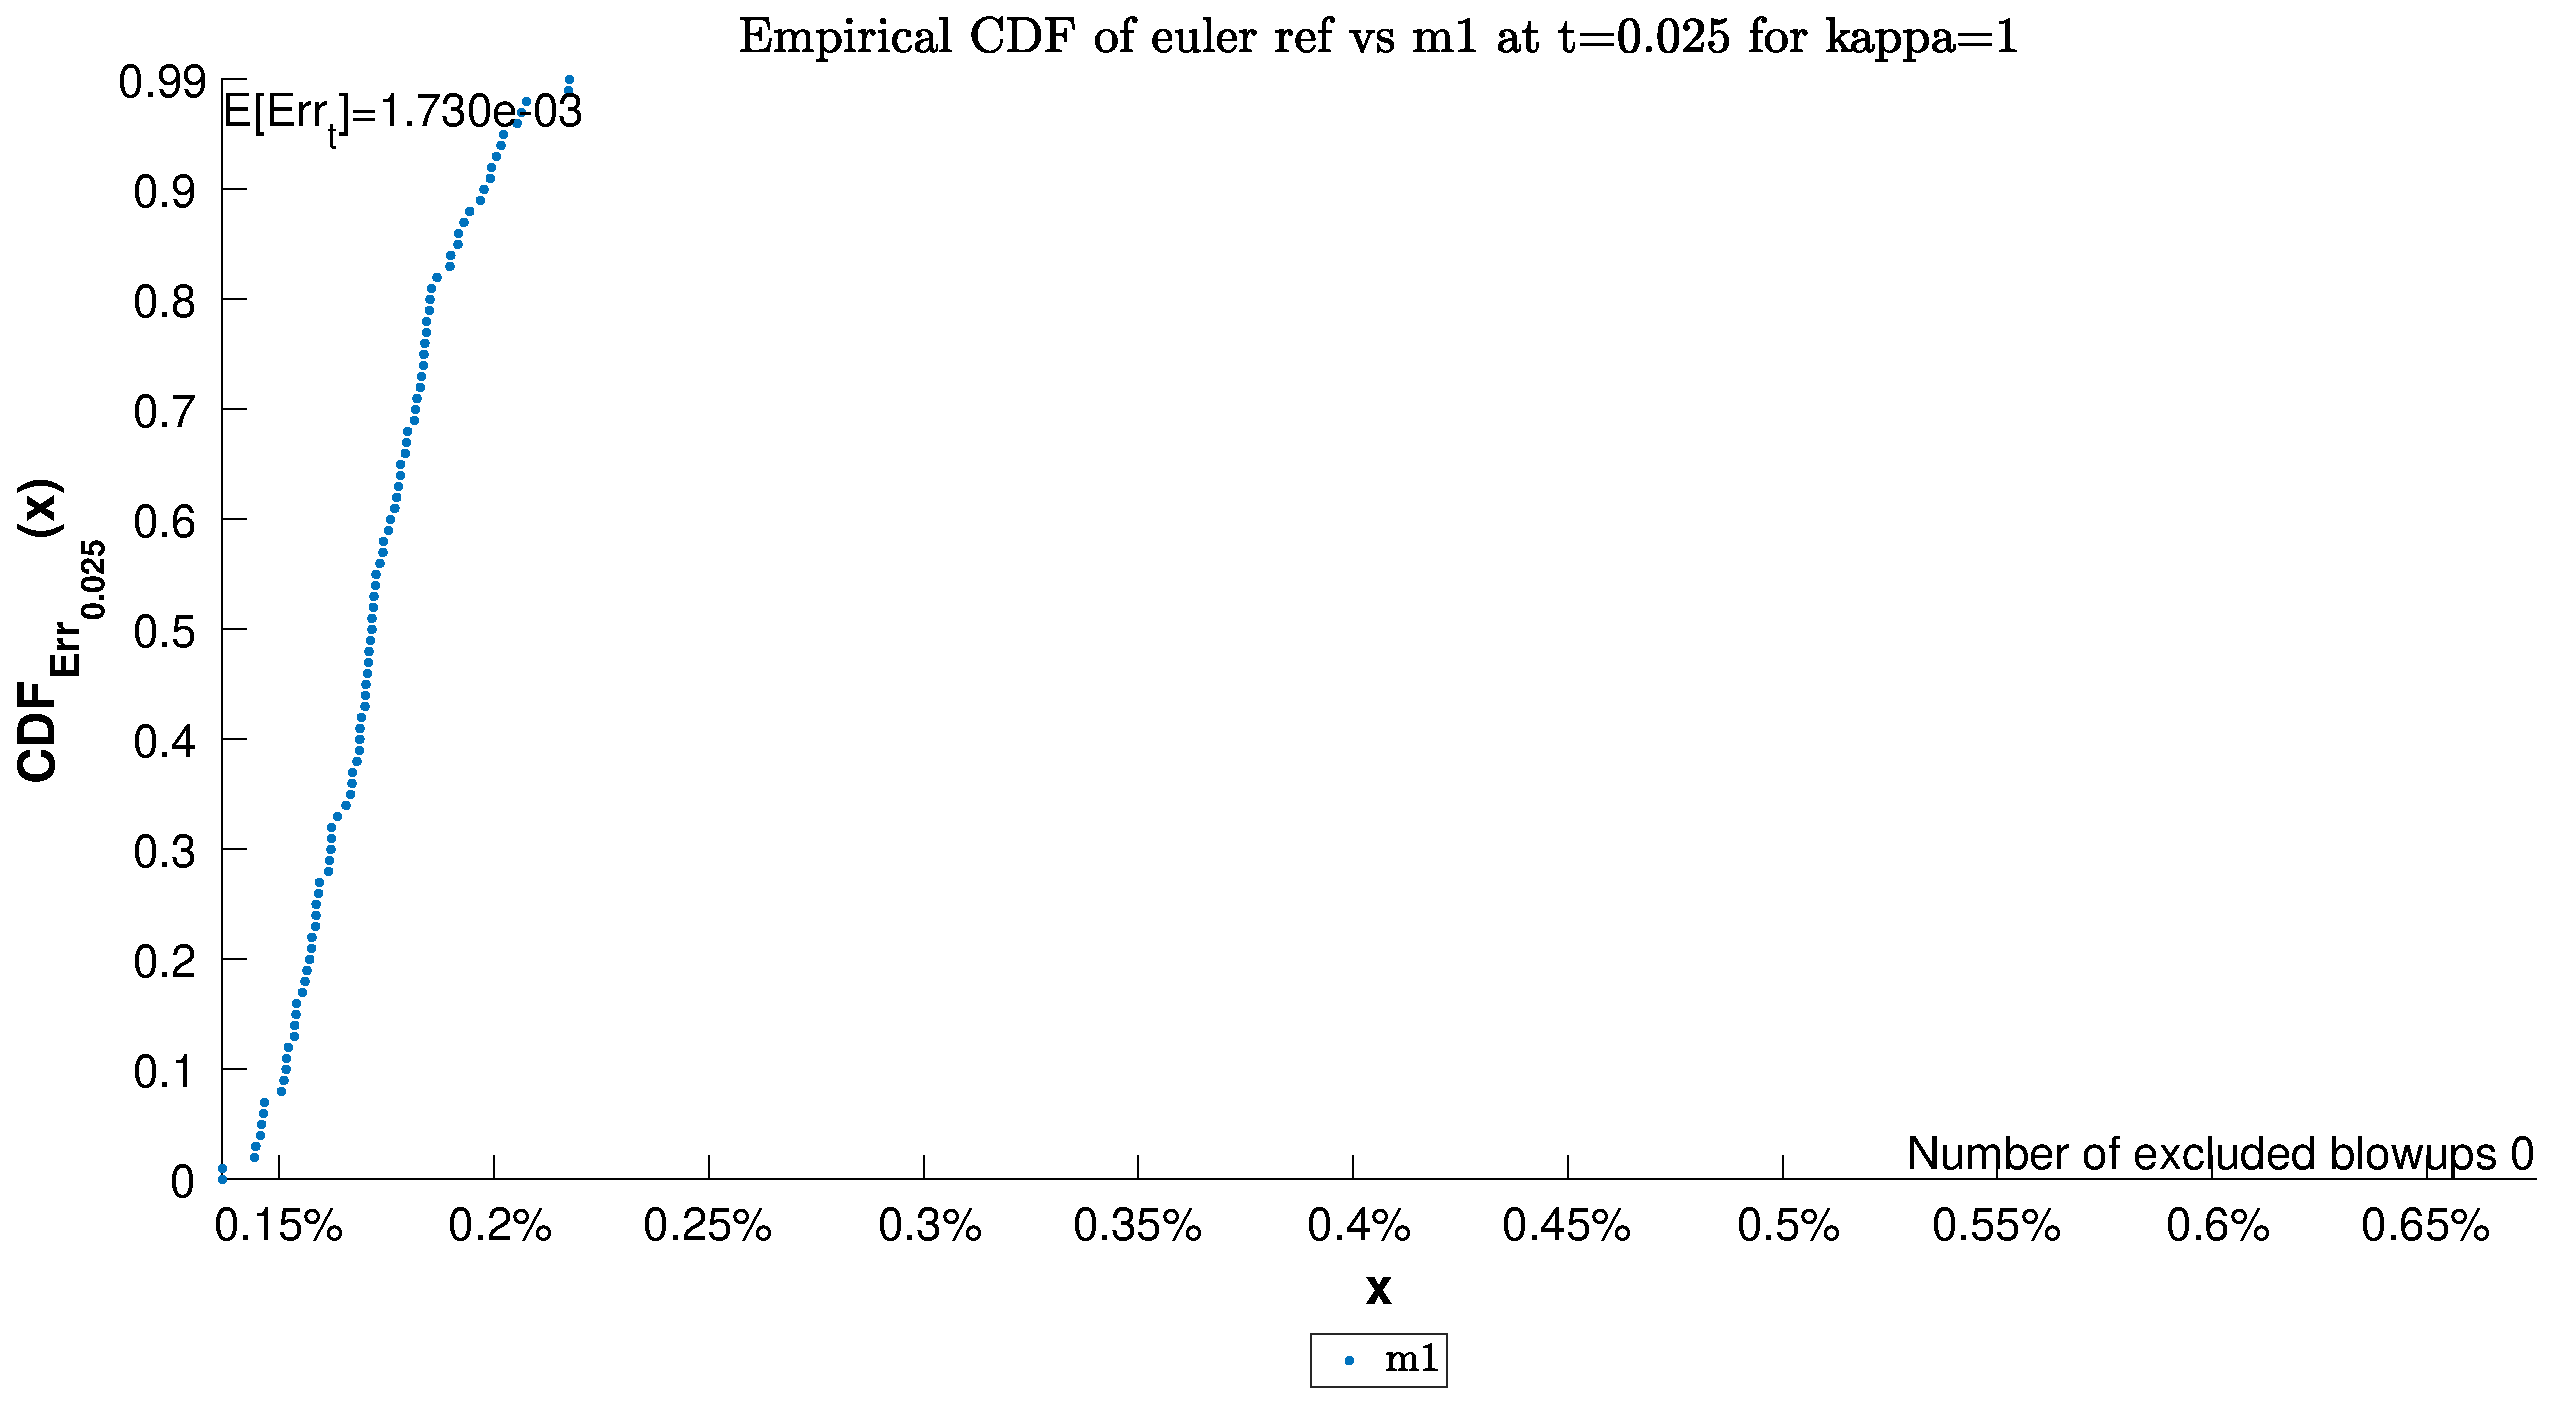
\includegraphics[width=.95\columnwidth]{CDF/CDFEulerRef_10}
\end{landscape}
\begin{landscape}
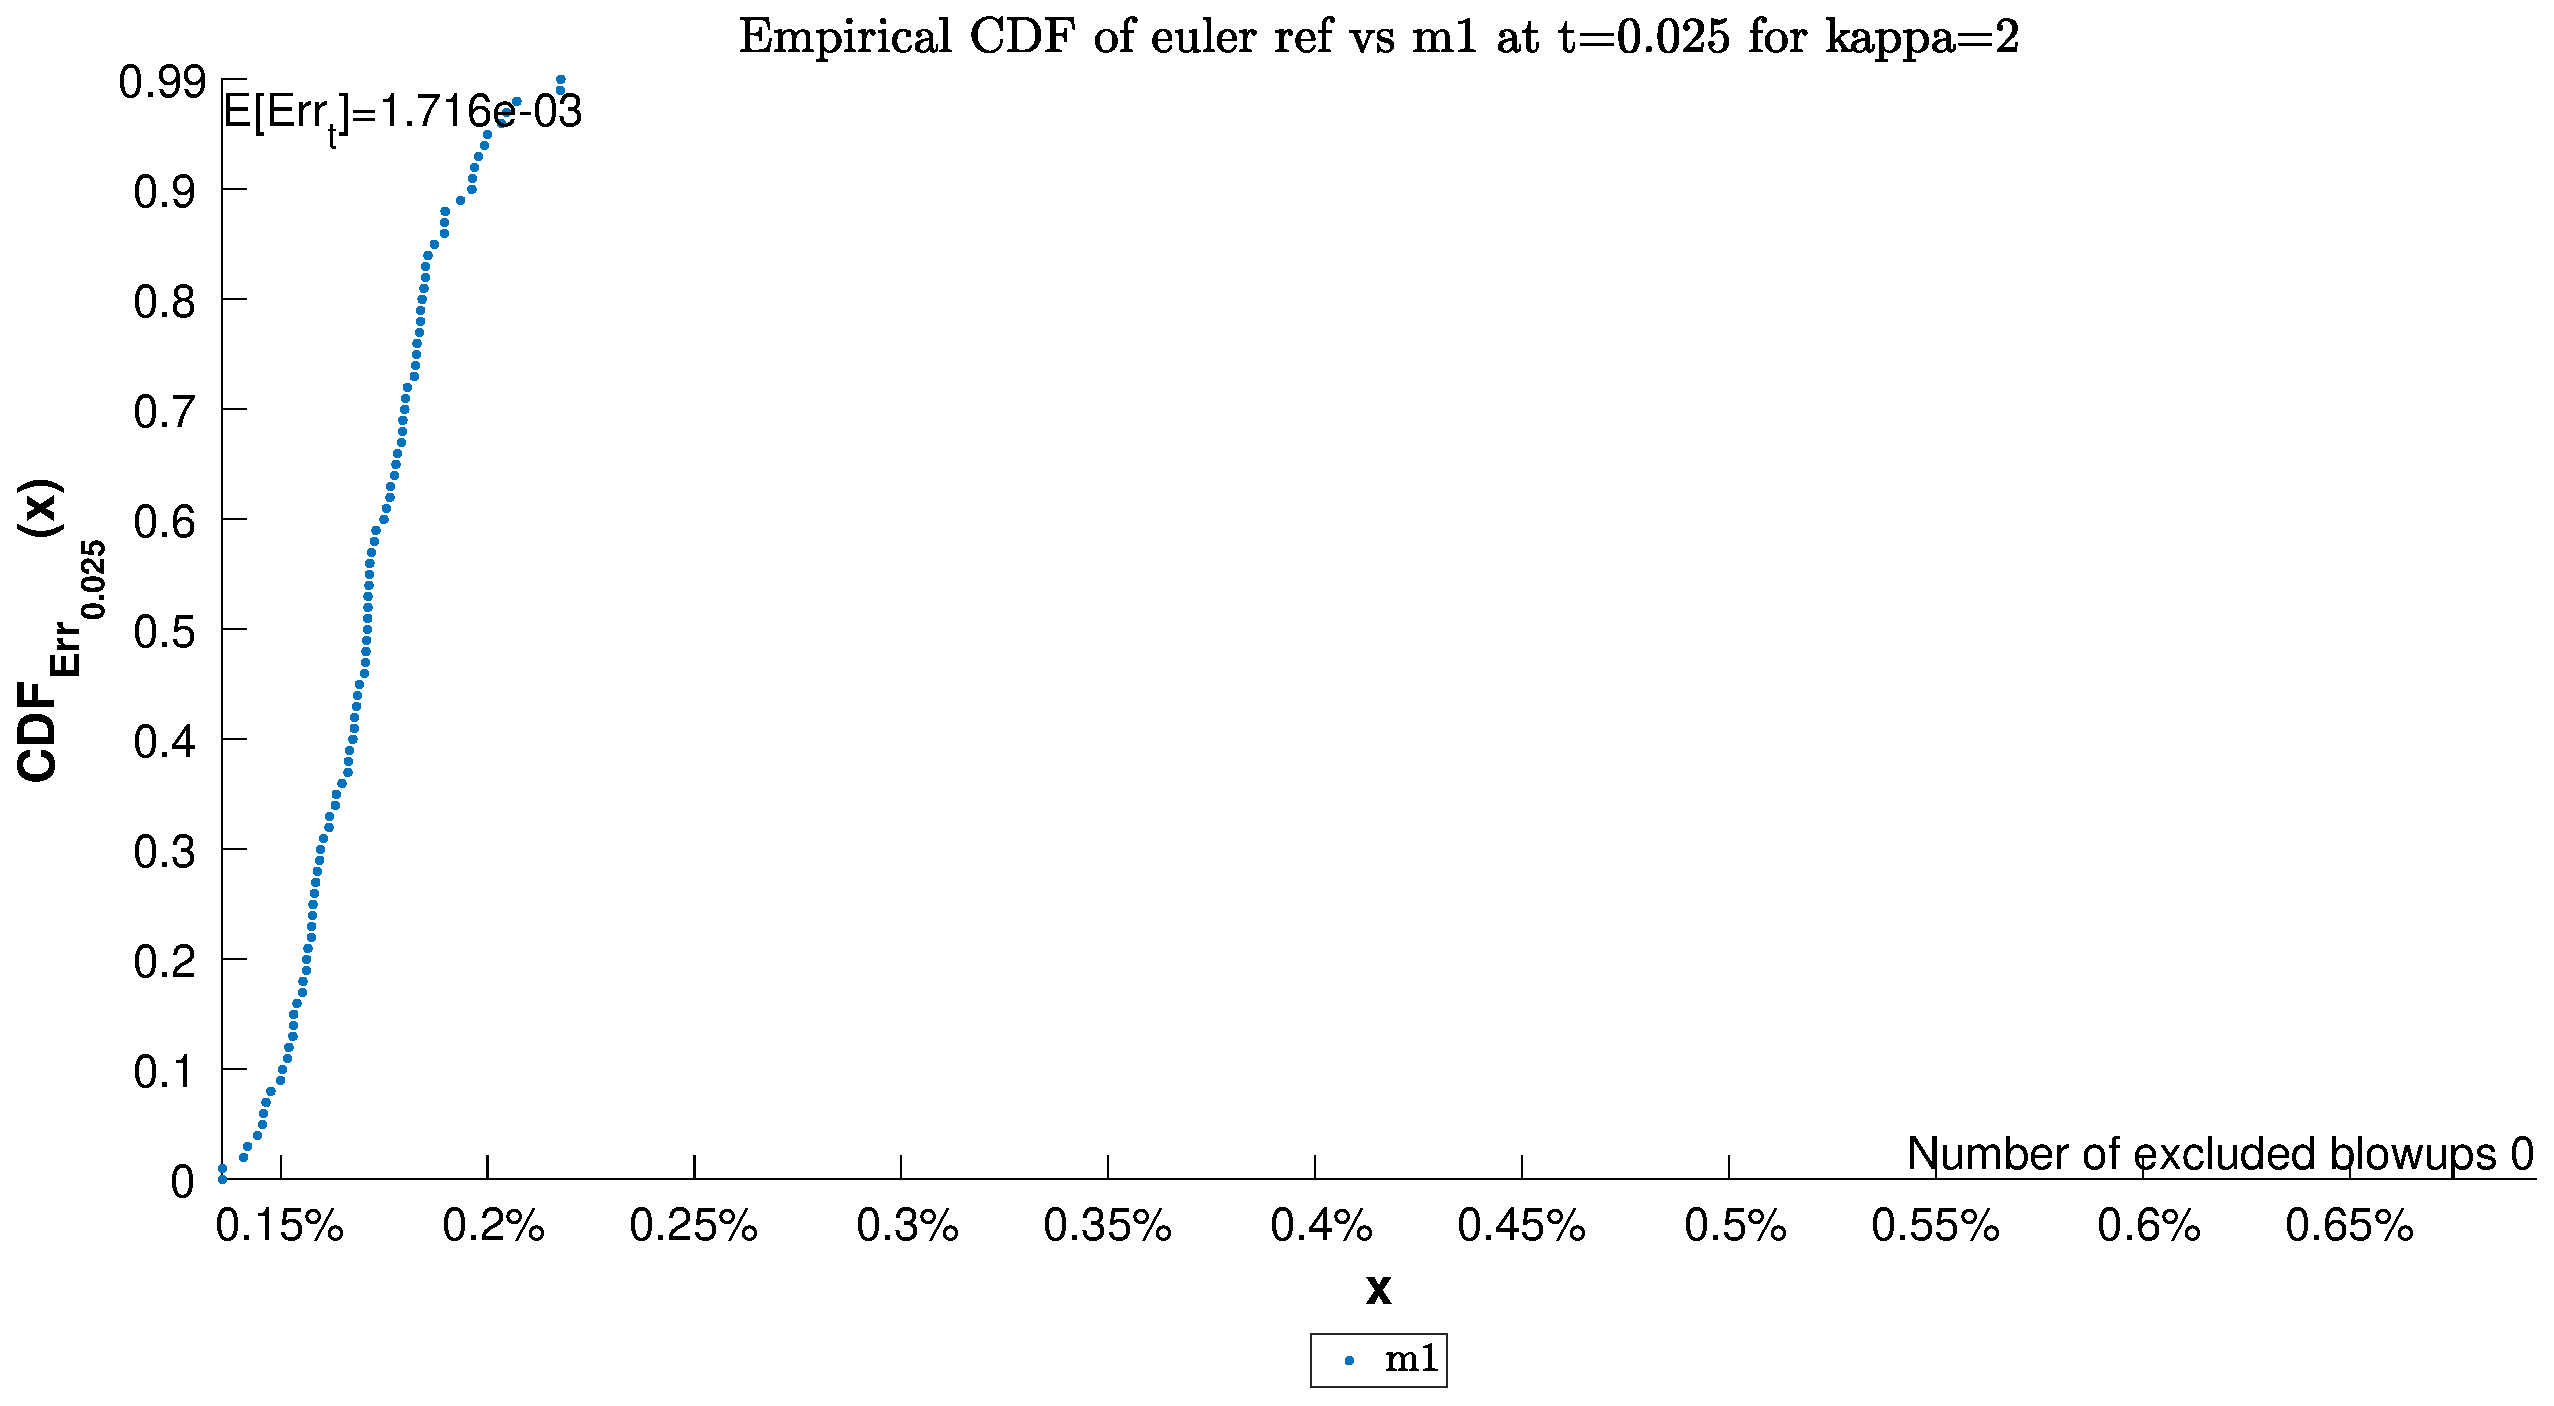
\includegraphics[width=.95\columnwidth]{CDF/CDFEulerRef_11}
\end{landscape}
\begin{landscape}
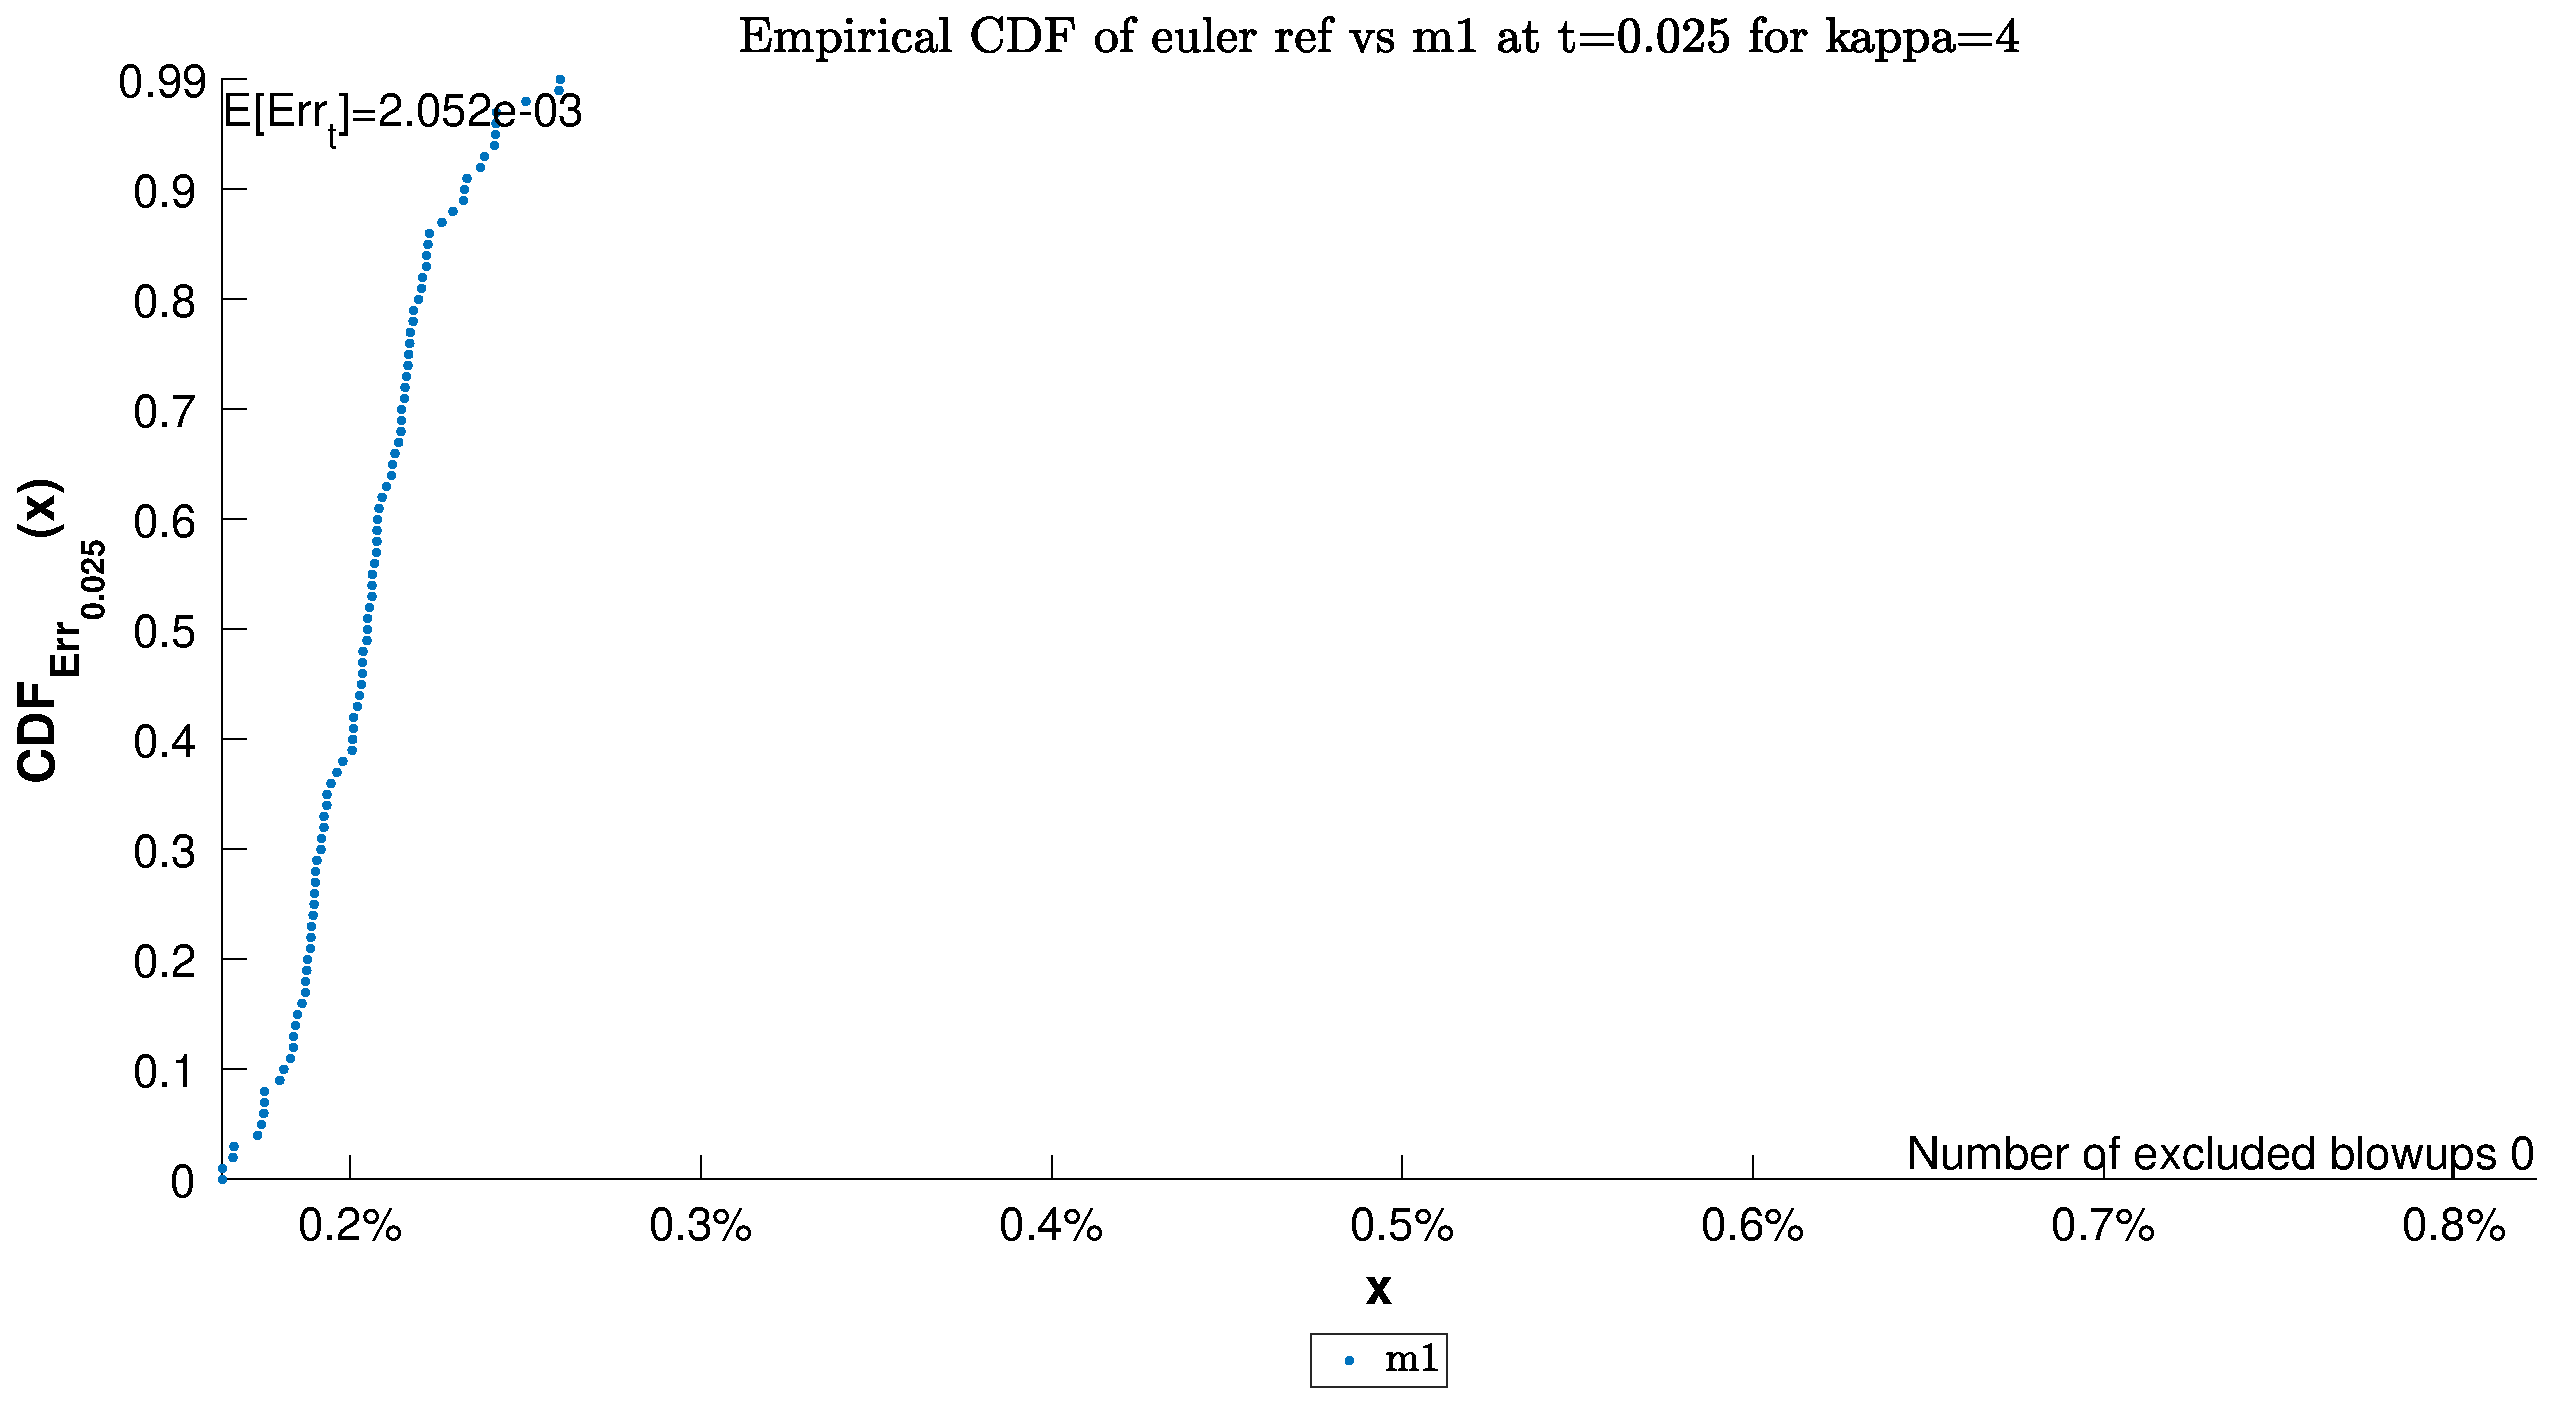
\includegraphics[width=.95\columnwidth]{CDF/CDFEulerRef_12}
\end{landscape}
\begin{landscape}
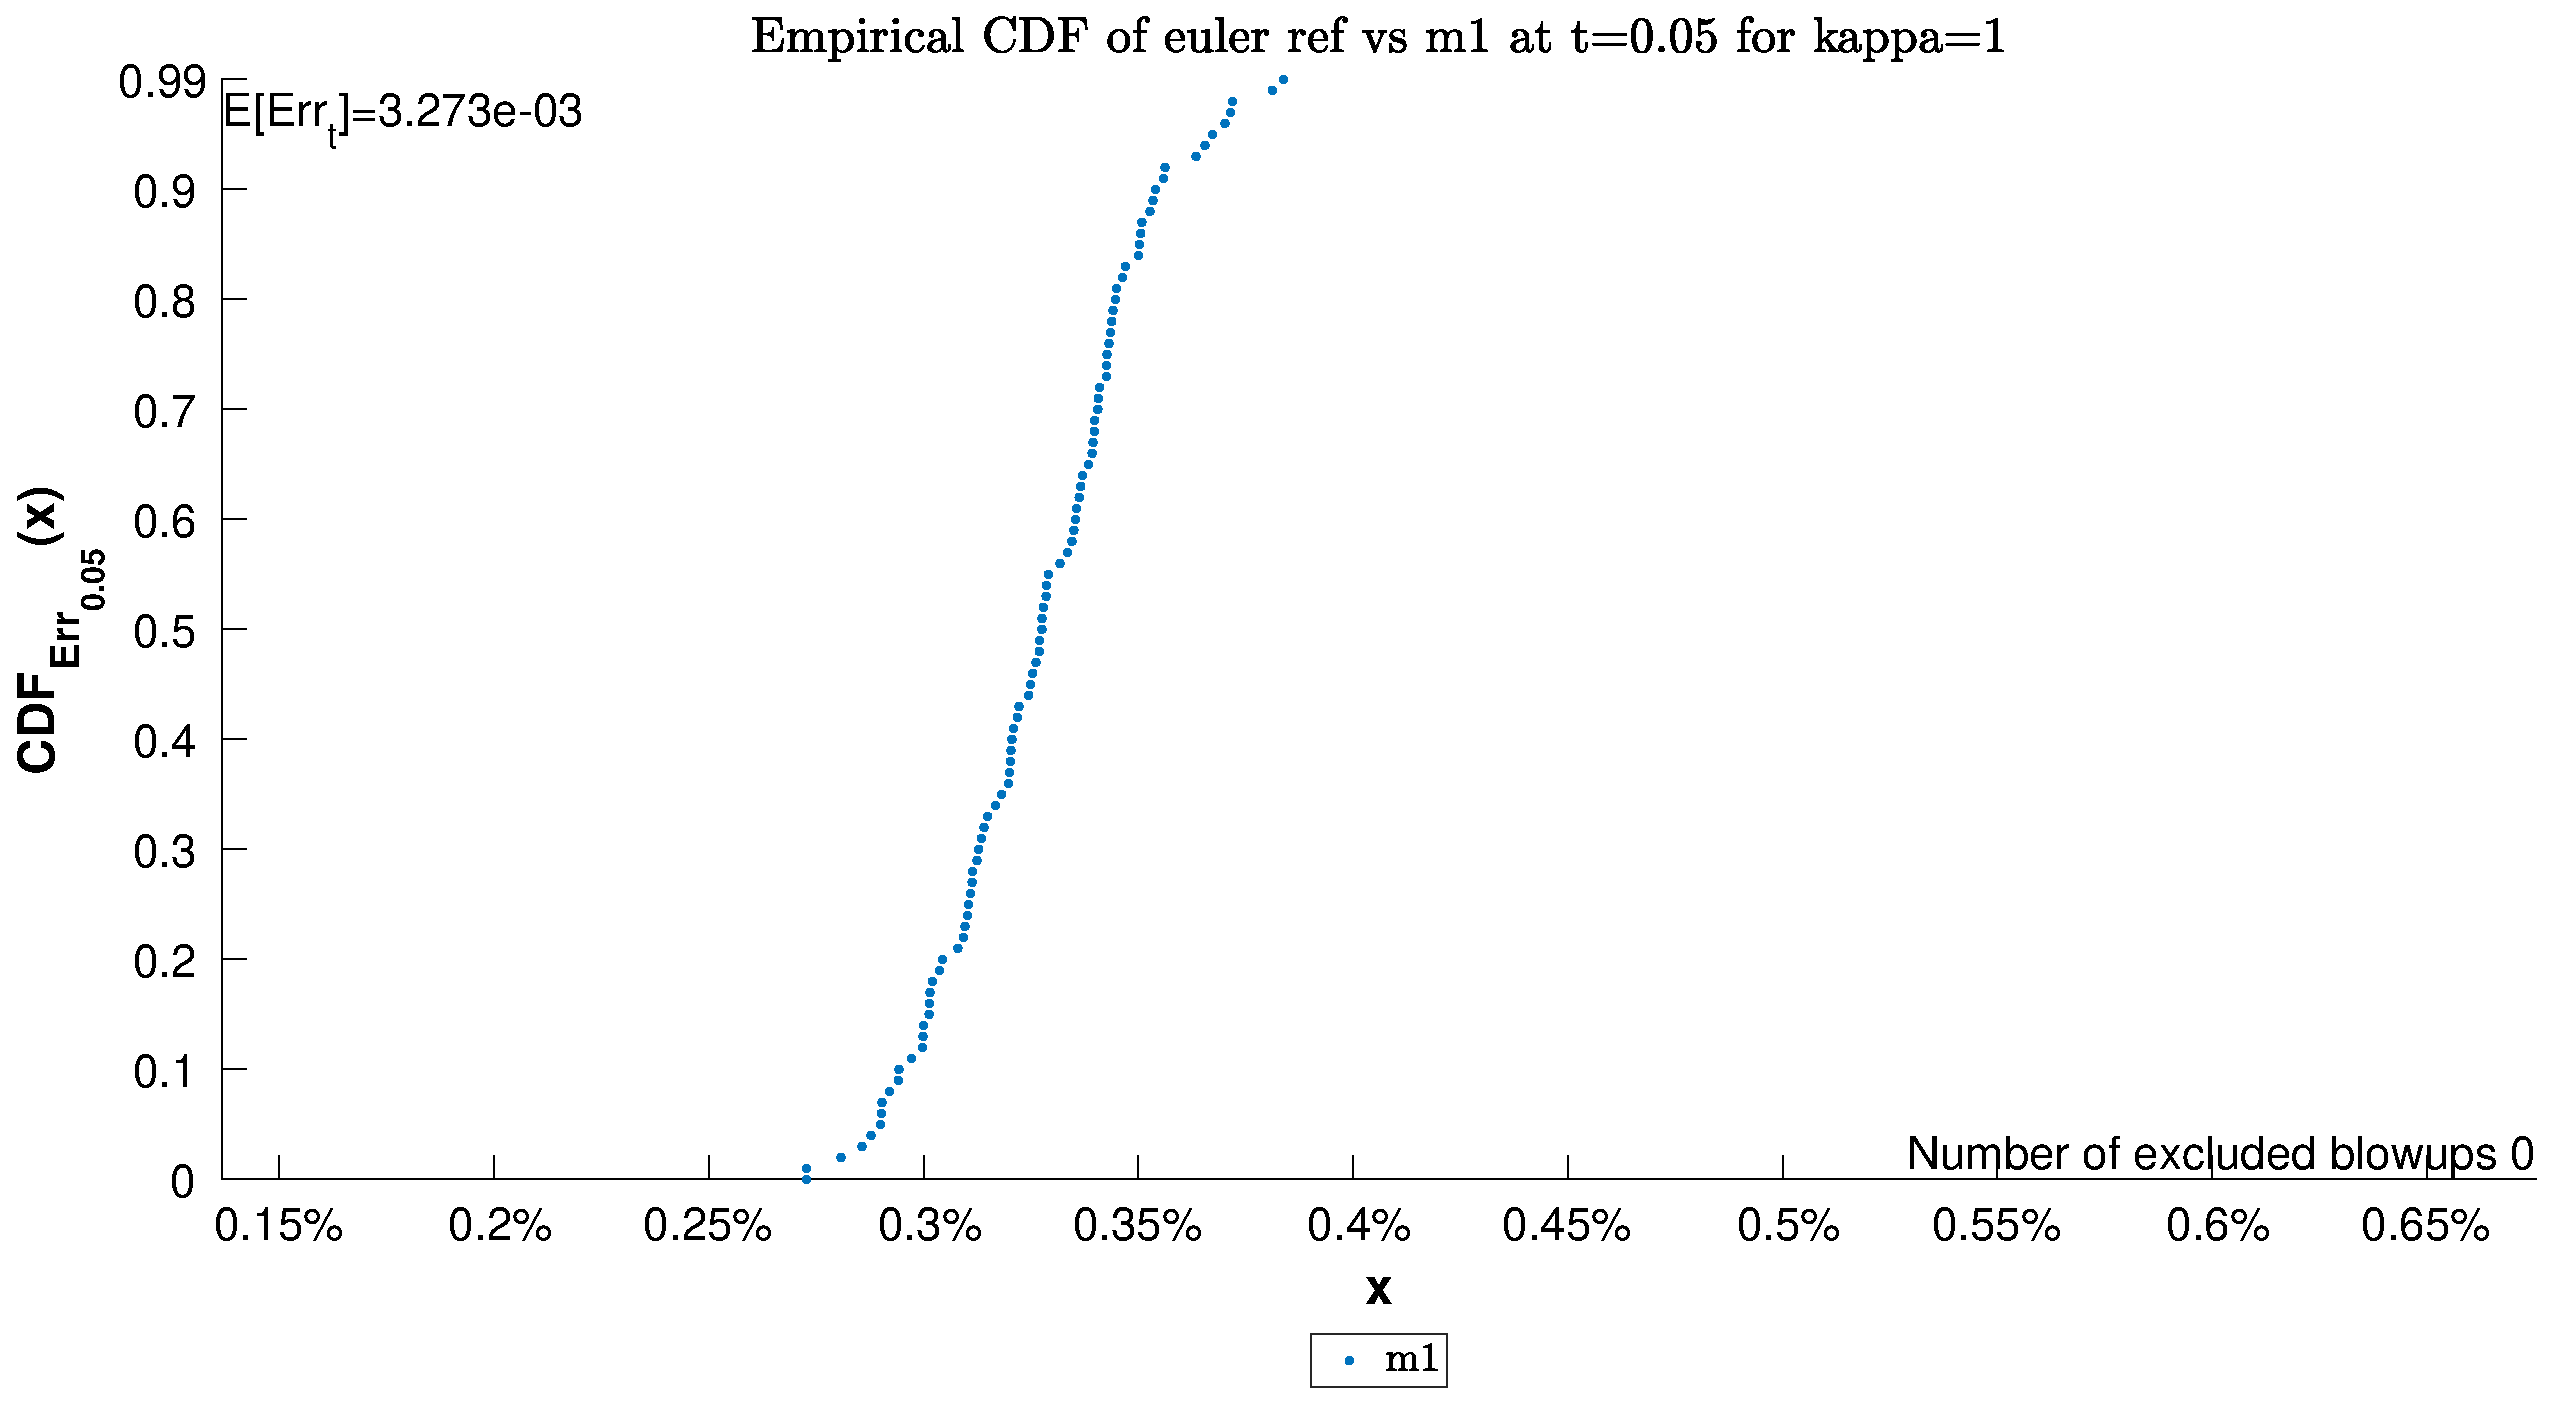
\includegraphics[width=.95\columnwidth]{CDF/CDFEulerRef_13}
\end{landscape}
\begin{landscape}
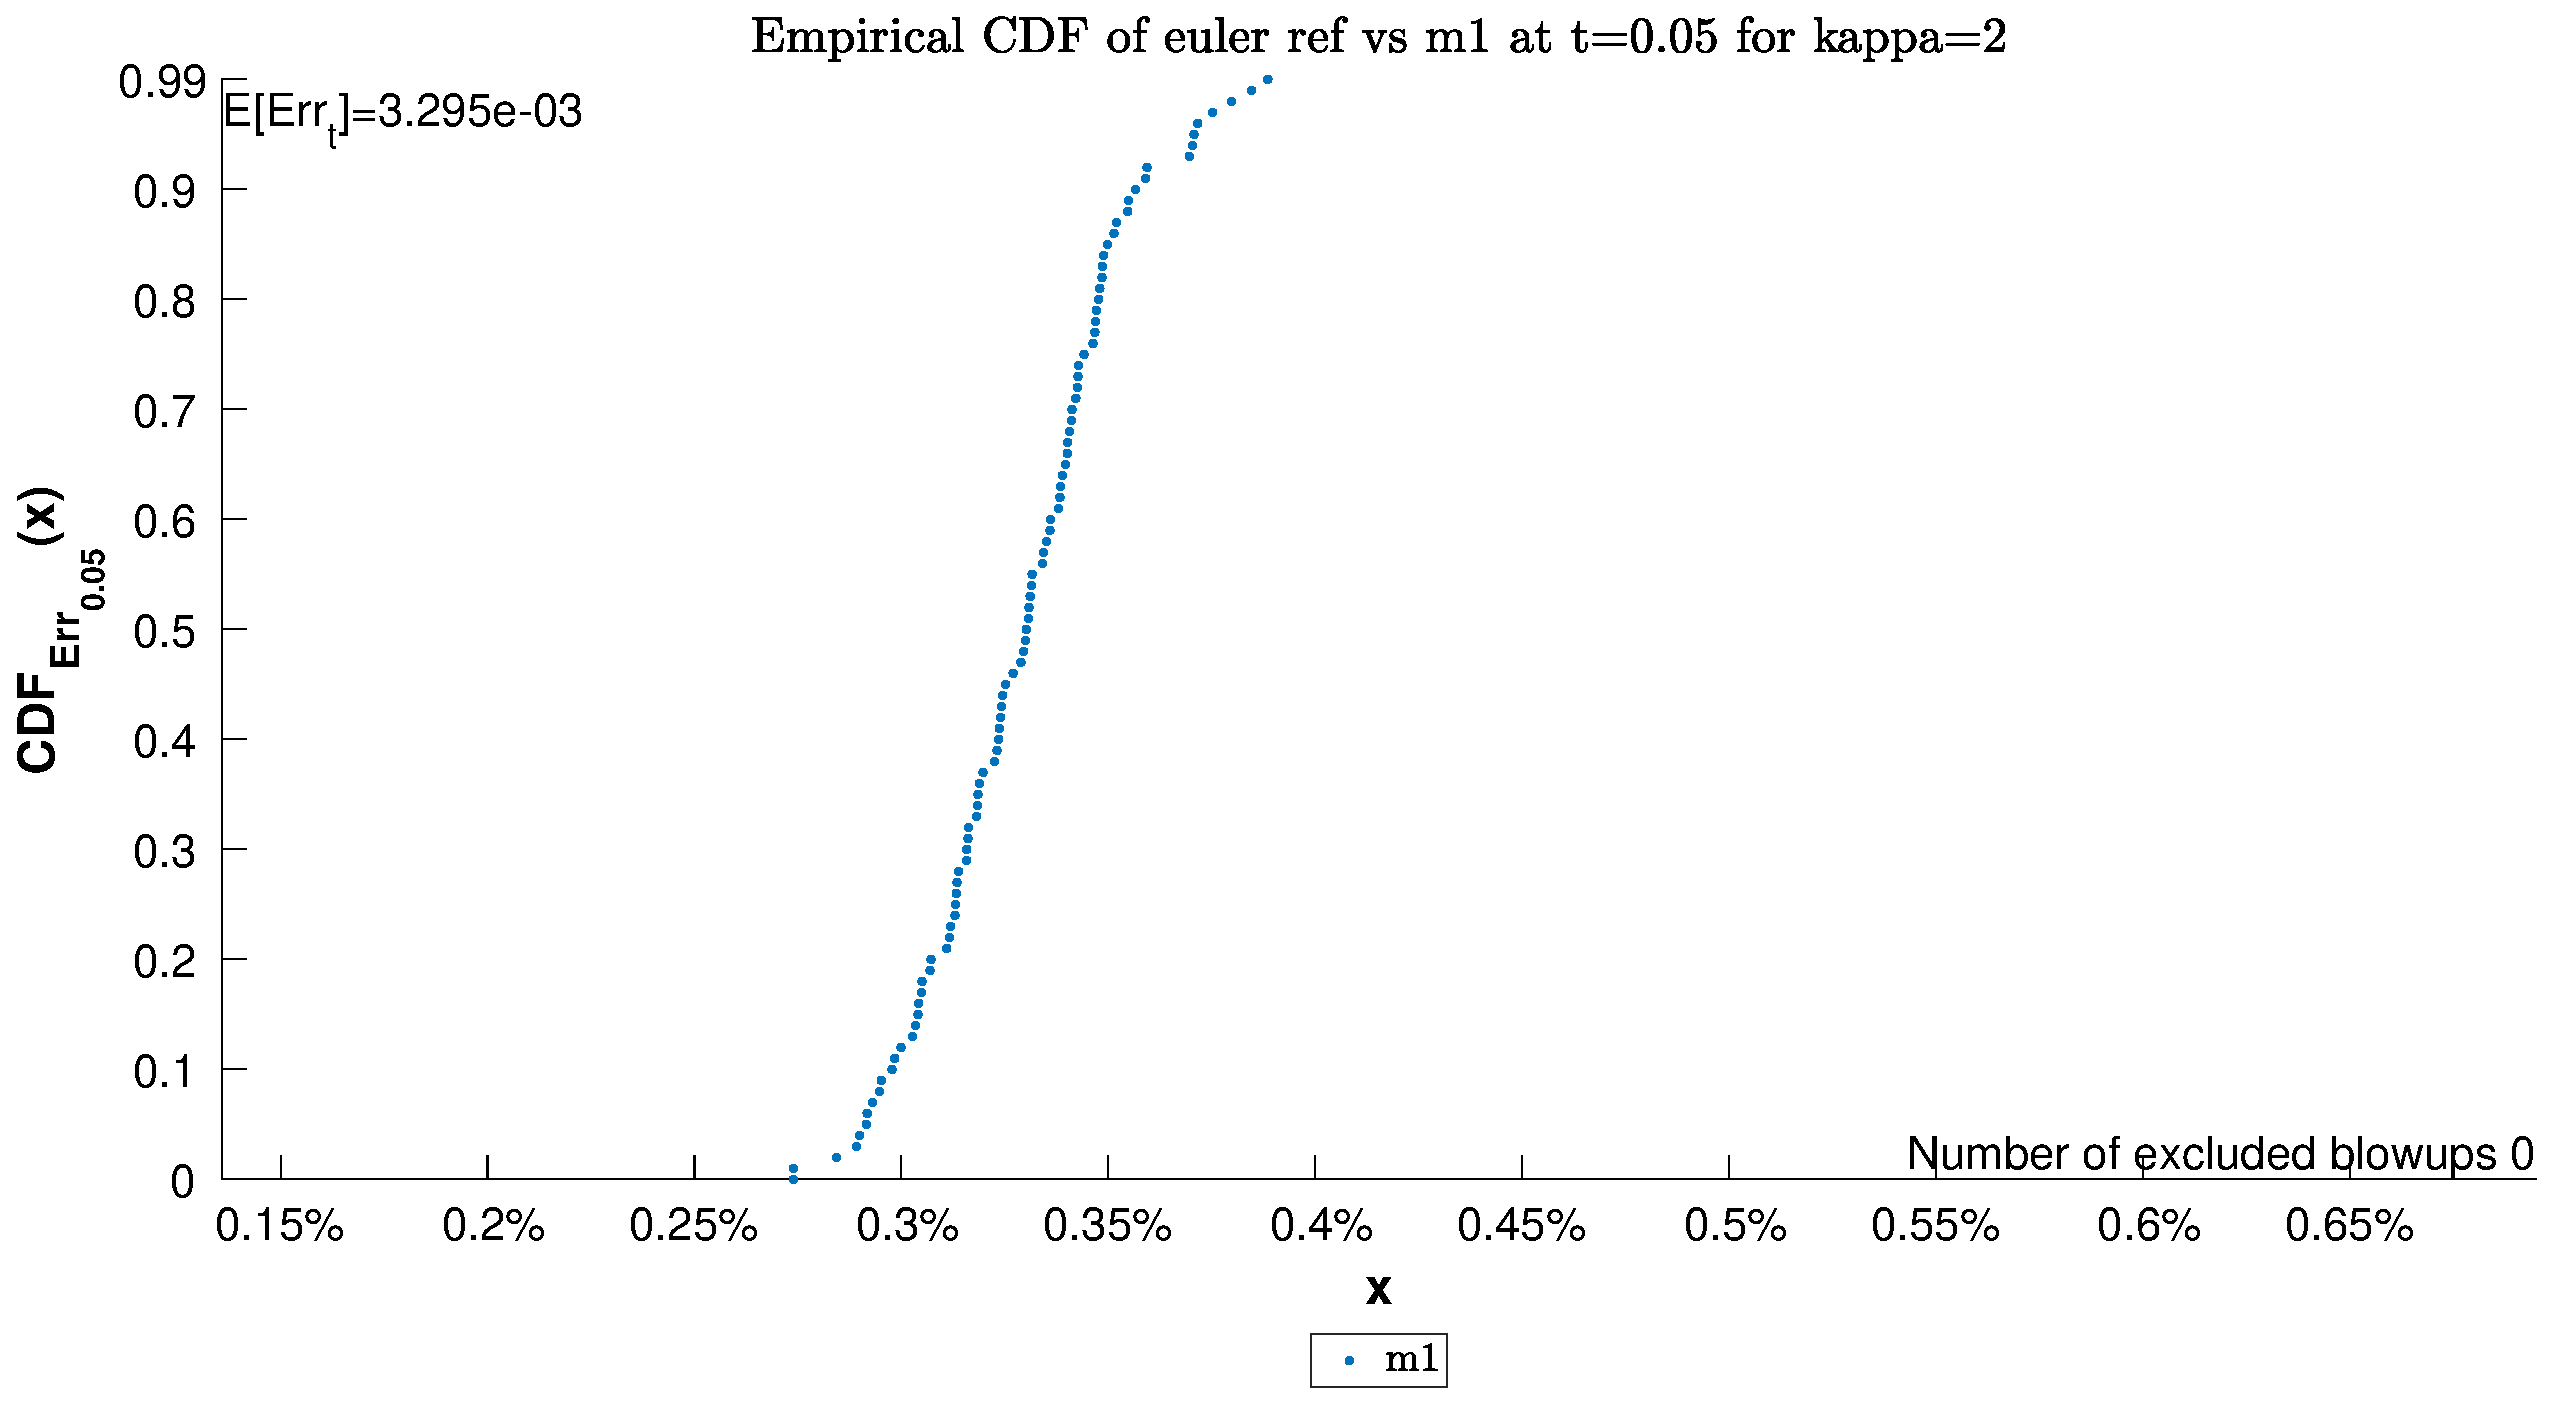
\includegraphics[width=.95\columnwidth]{CDF/CDFEulerRef_14}
\end{landscape}
\begin{landscape}
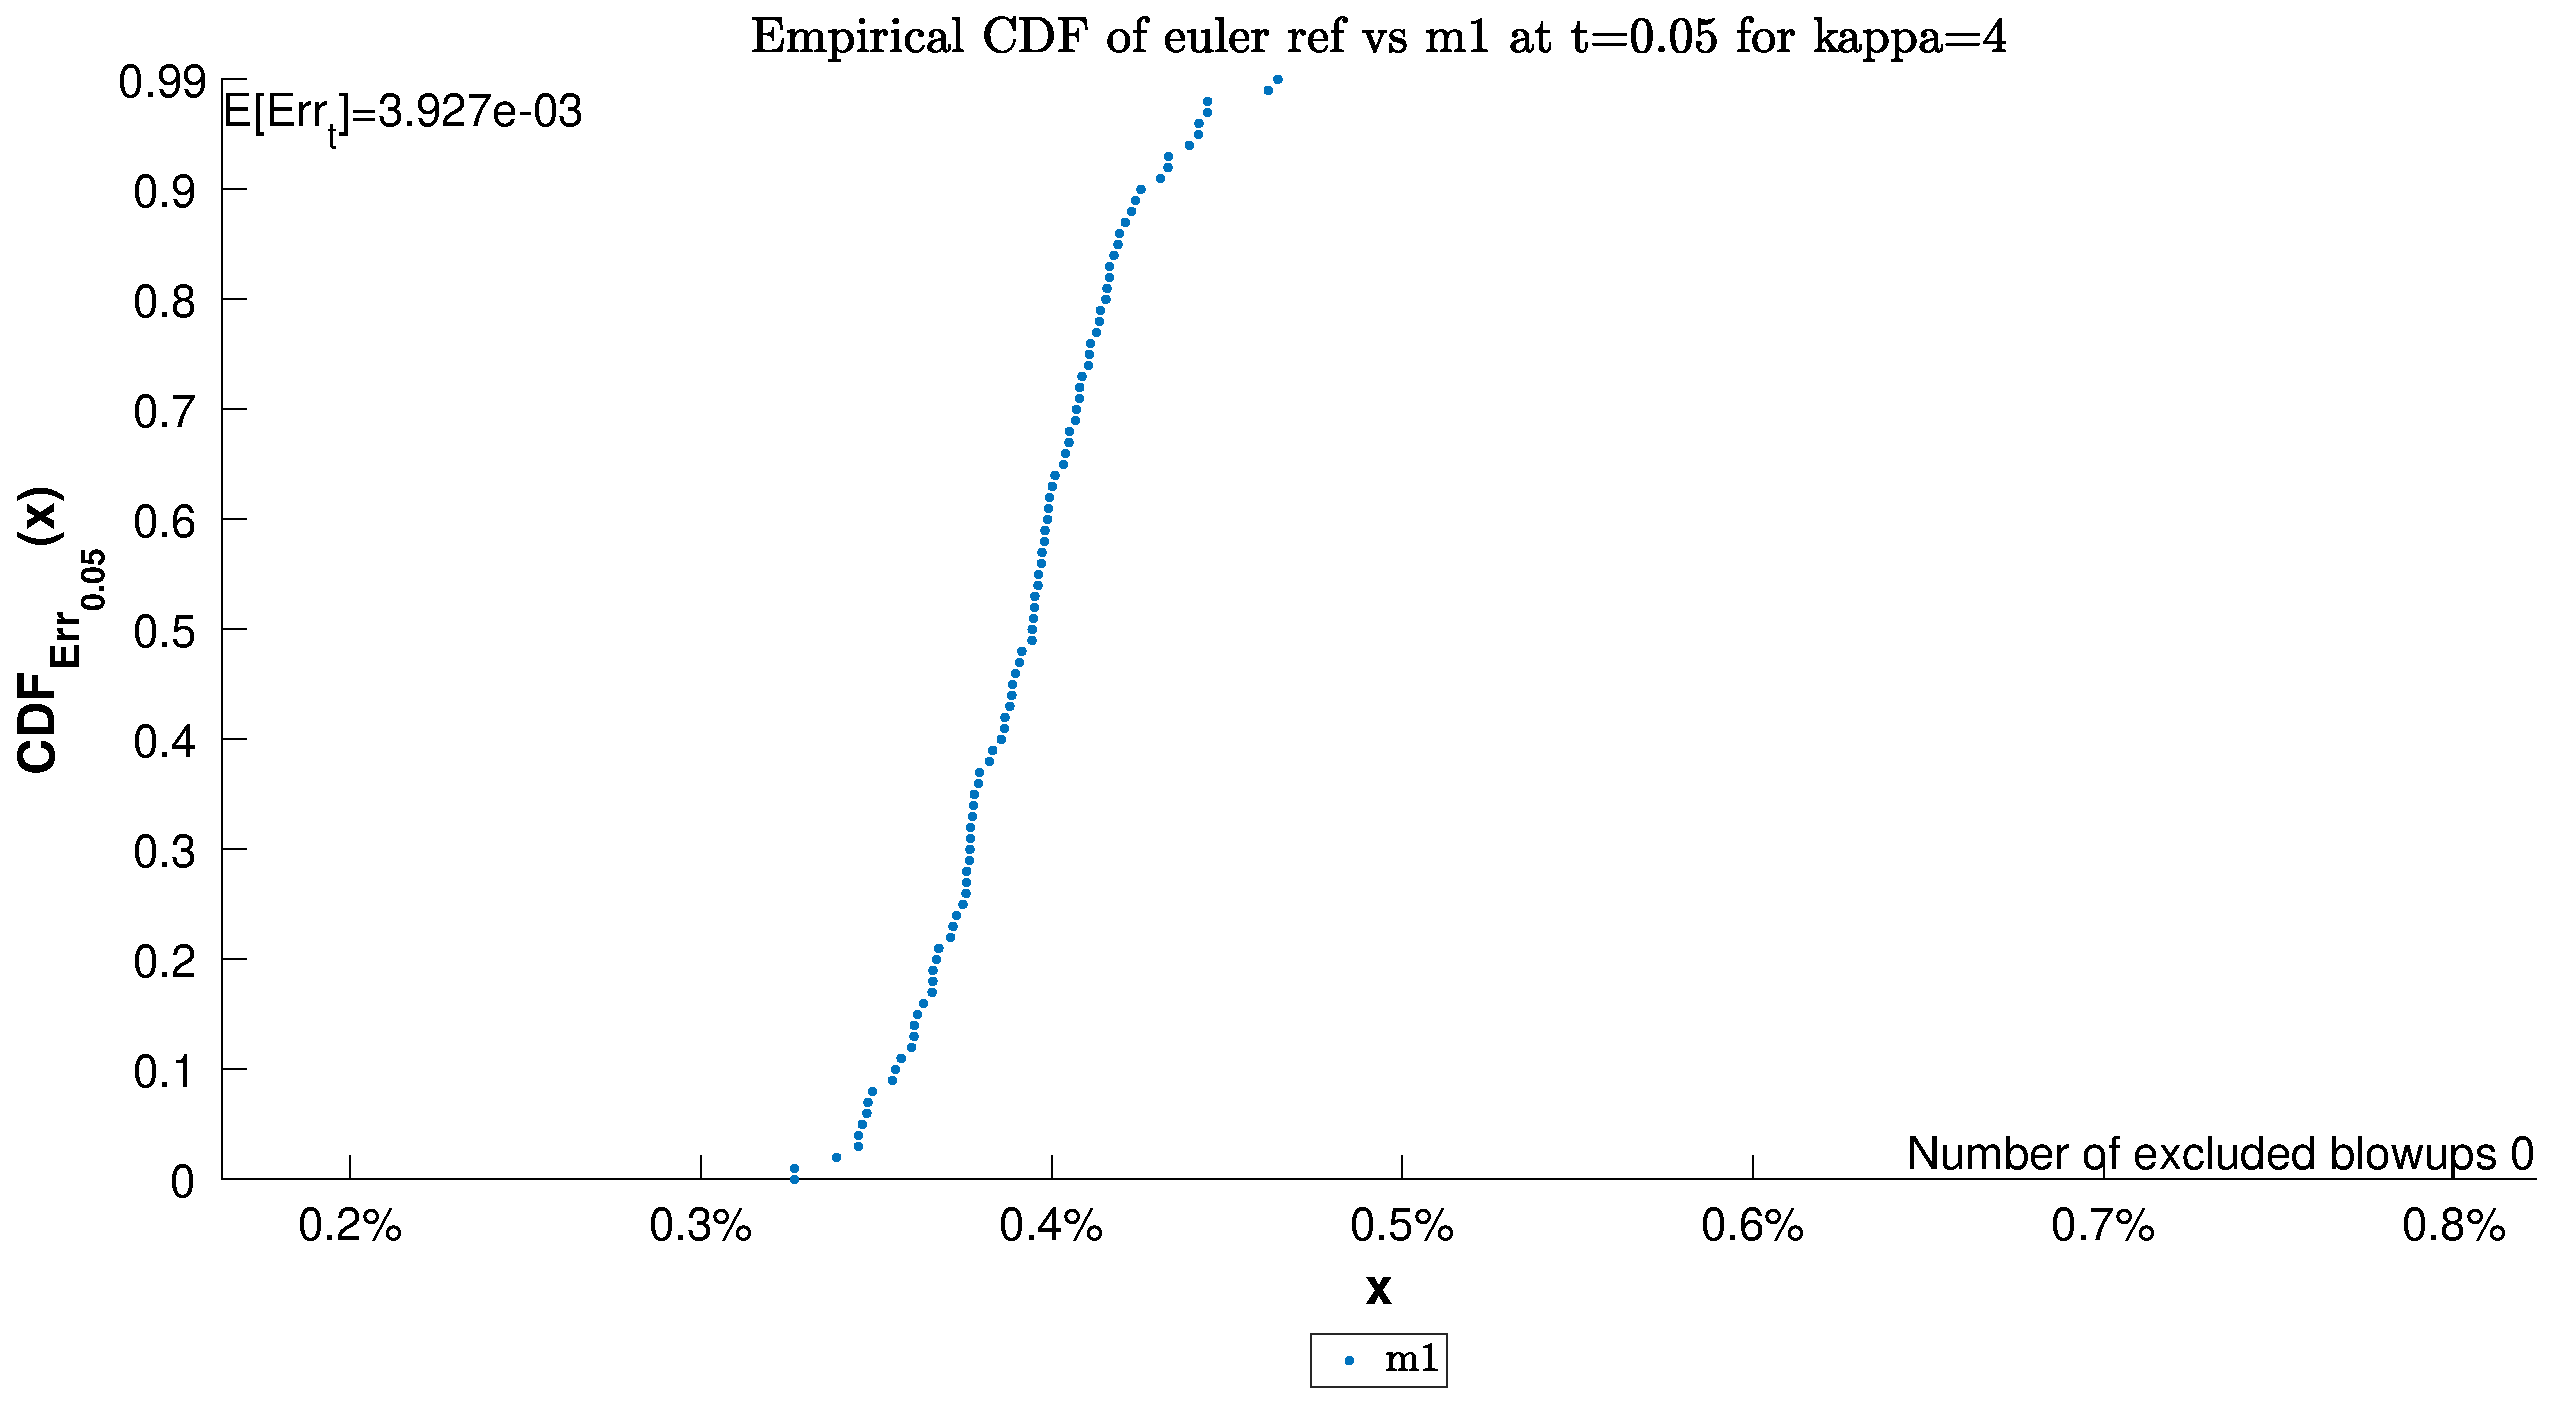
\includegraphics[width=.95\columnwidth]{CDF/CDFEulerRef_15}
\end{landscape}
\begin{landscape}
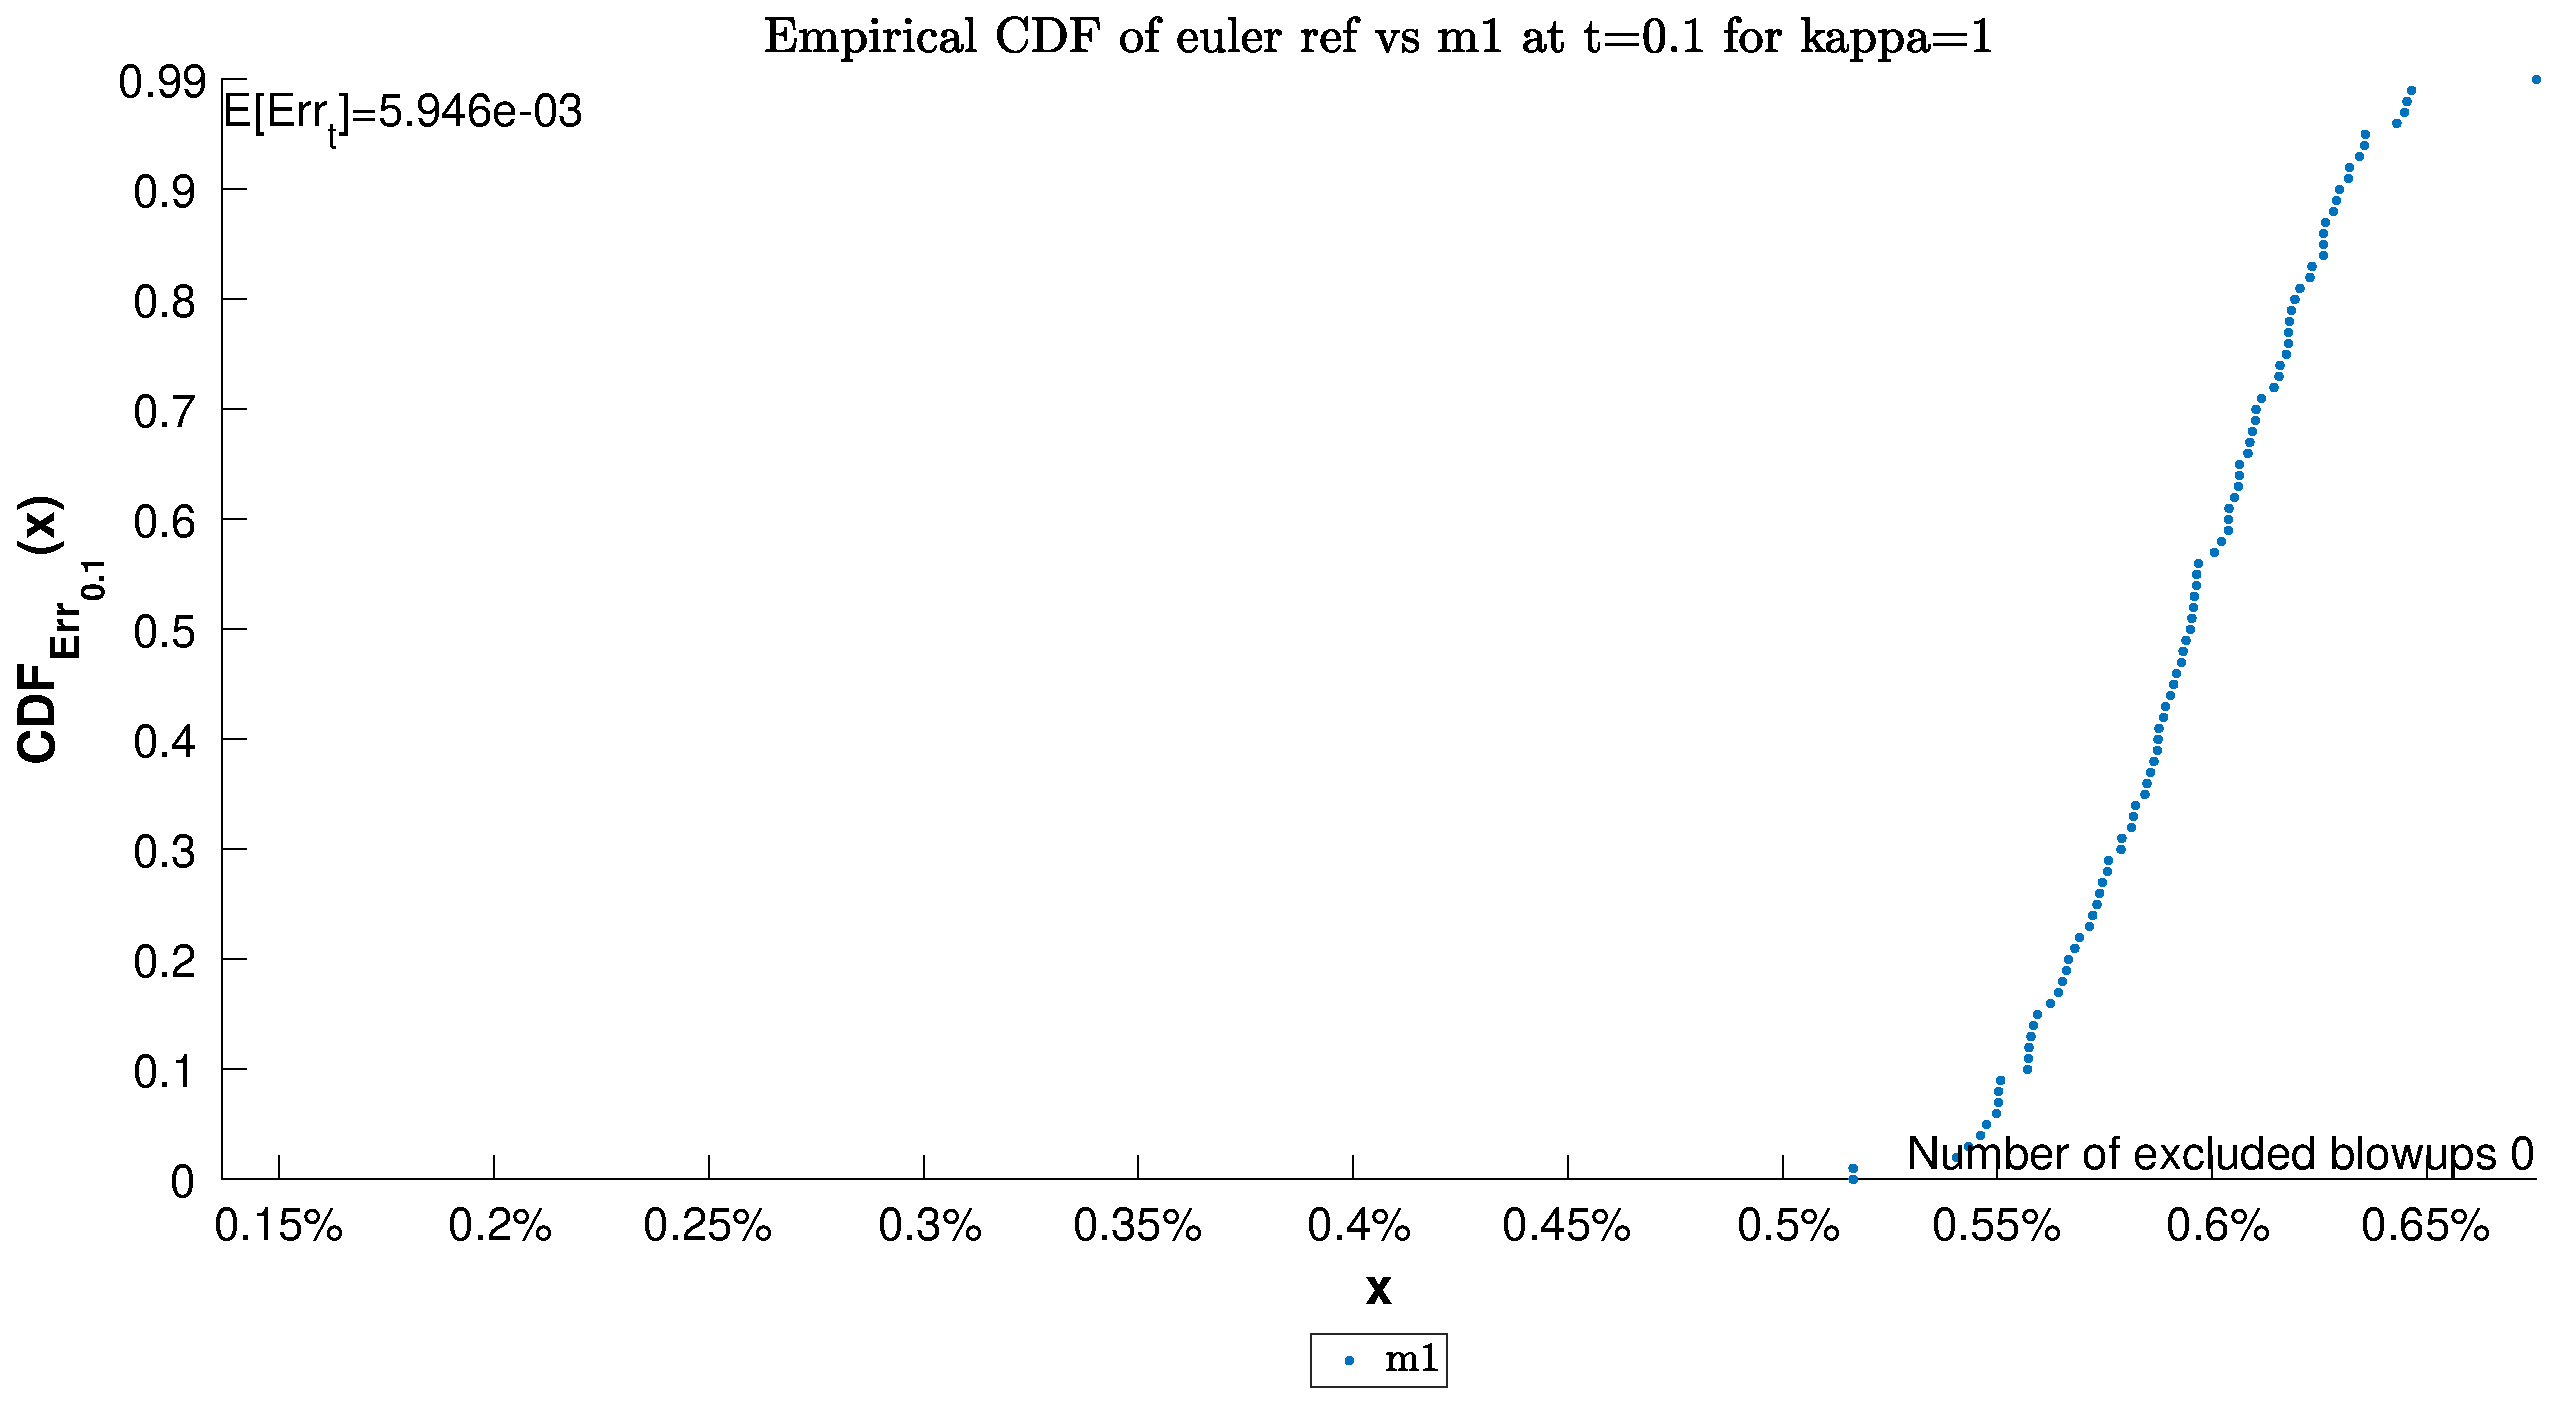
\includegraphics[width=.95\columnwidth]{CDF/CDFEulerRef_16}
\end{landscape}
\begin{landscape}
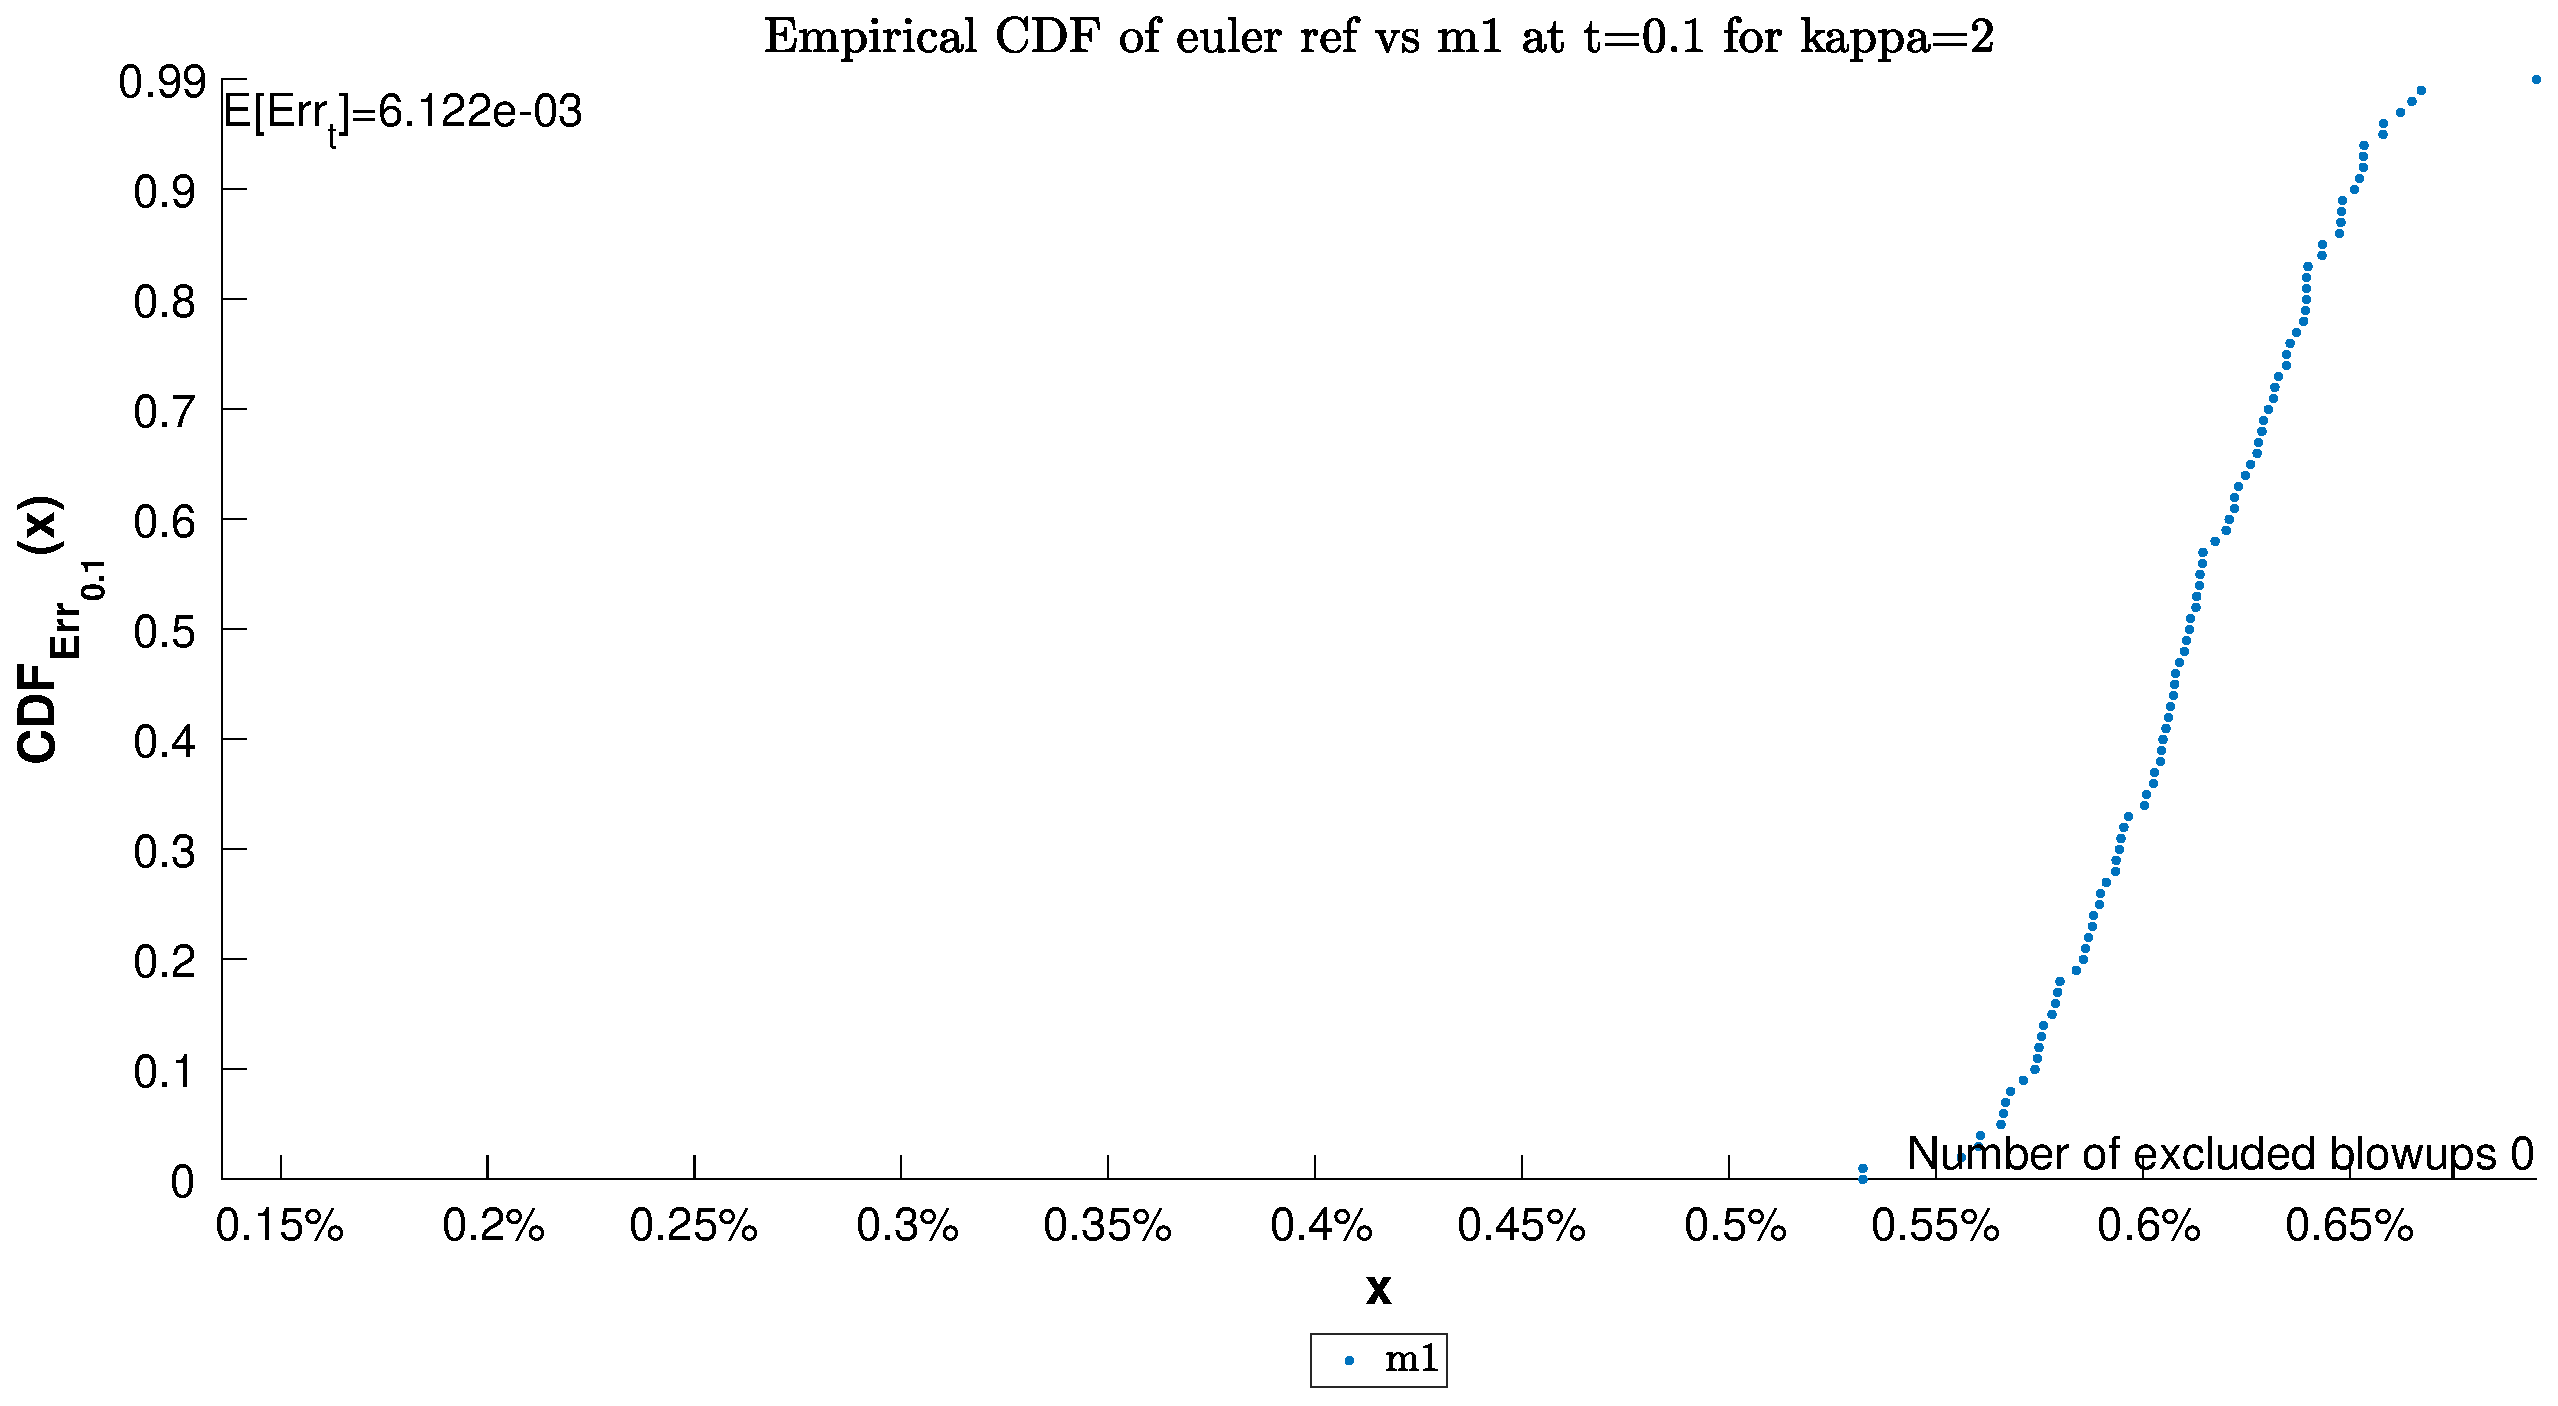
\includegraphics[width=.95\columnwidth]{CDF/CDFEulerRef_17}
\end{landscape}
\begin{landscape}
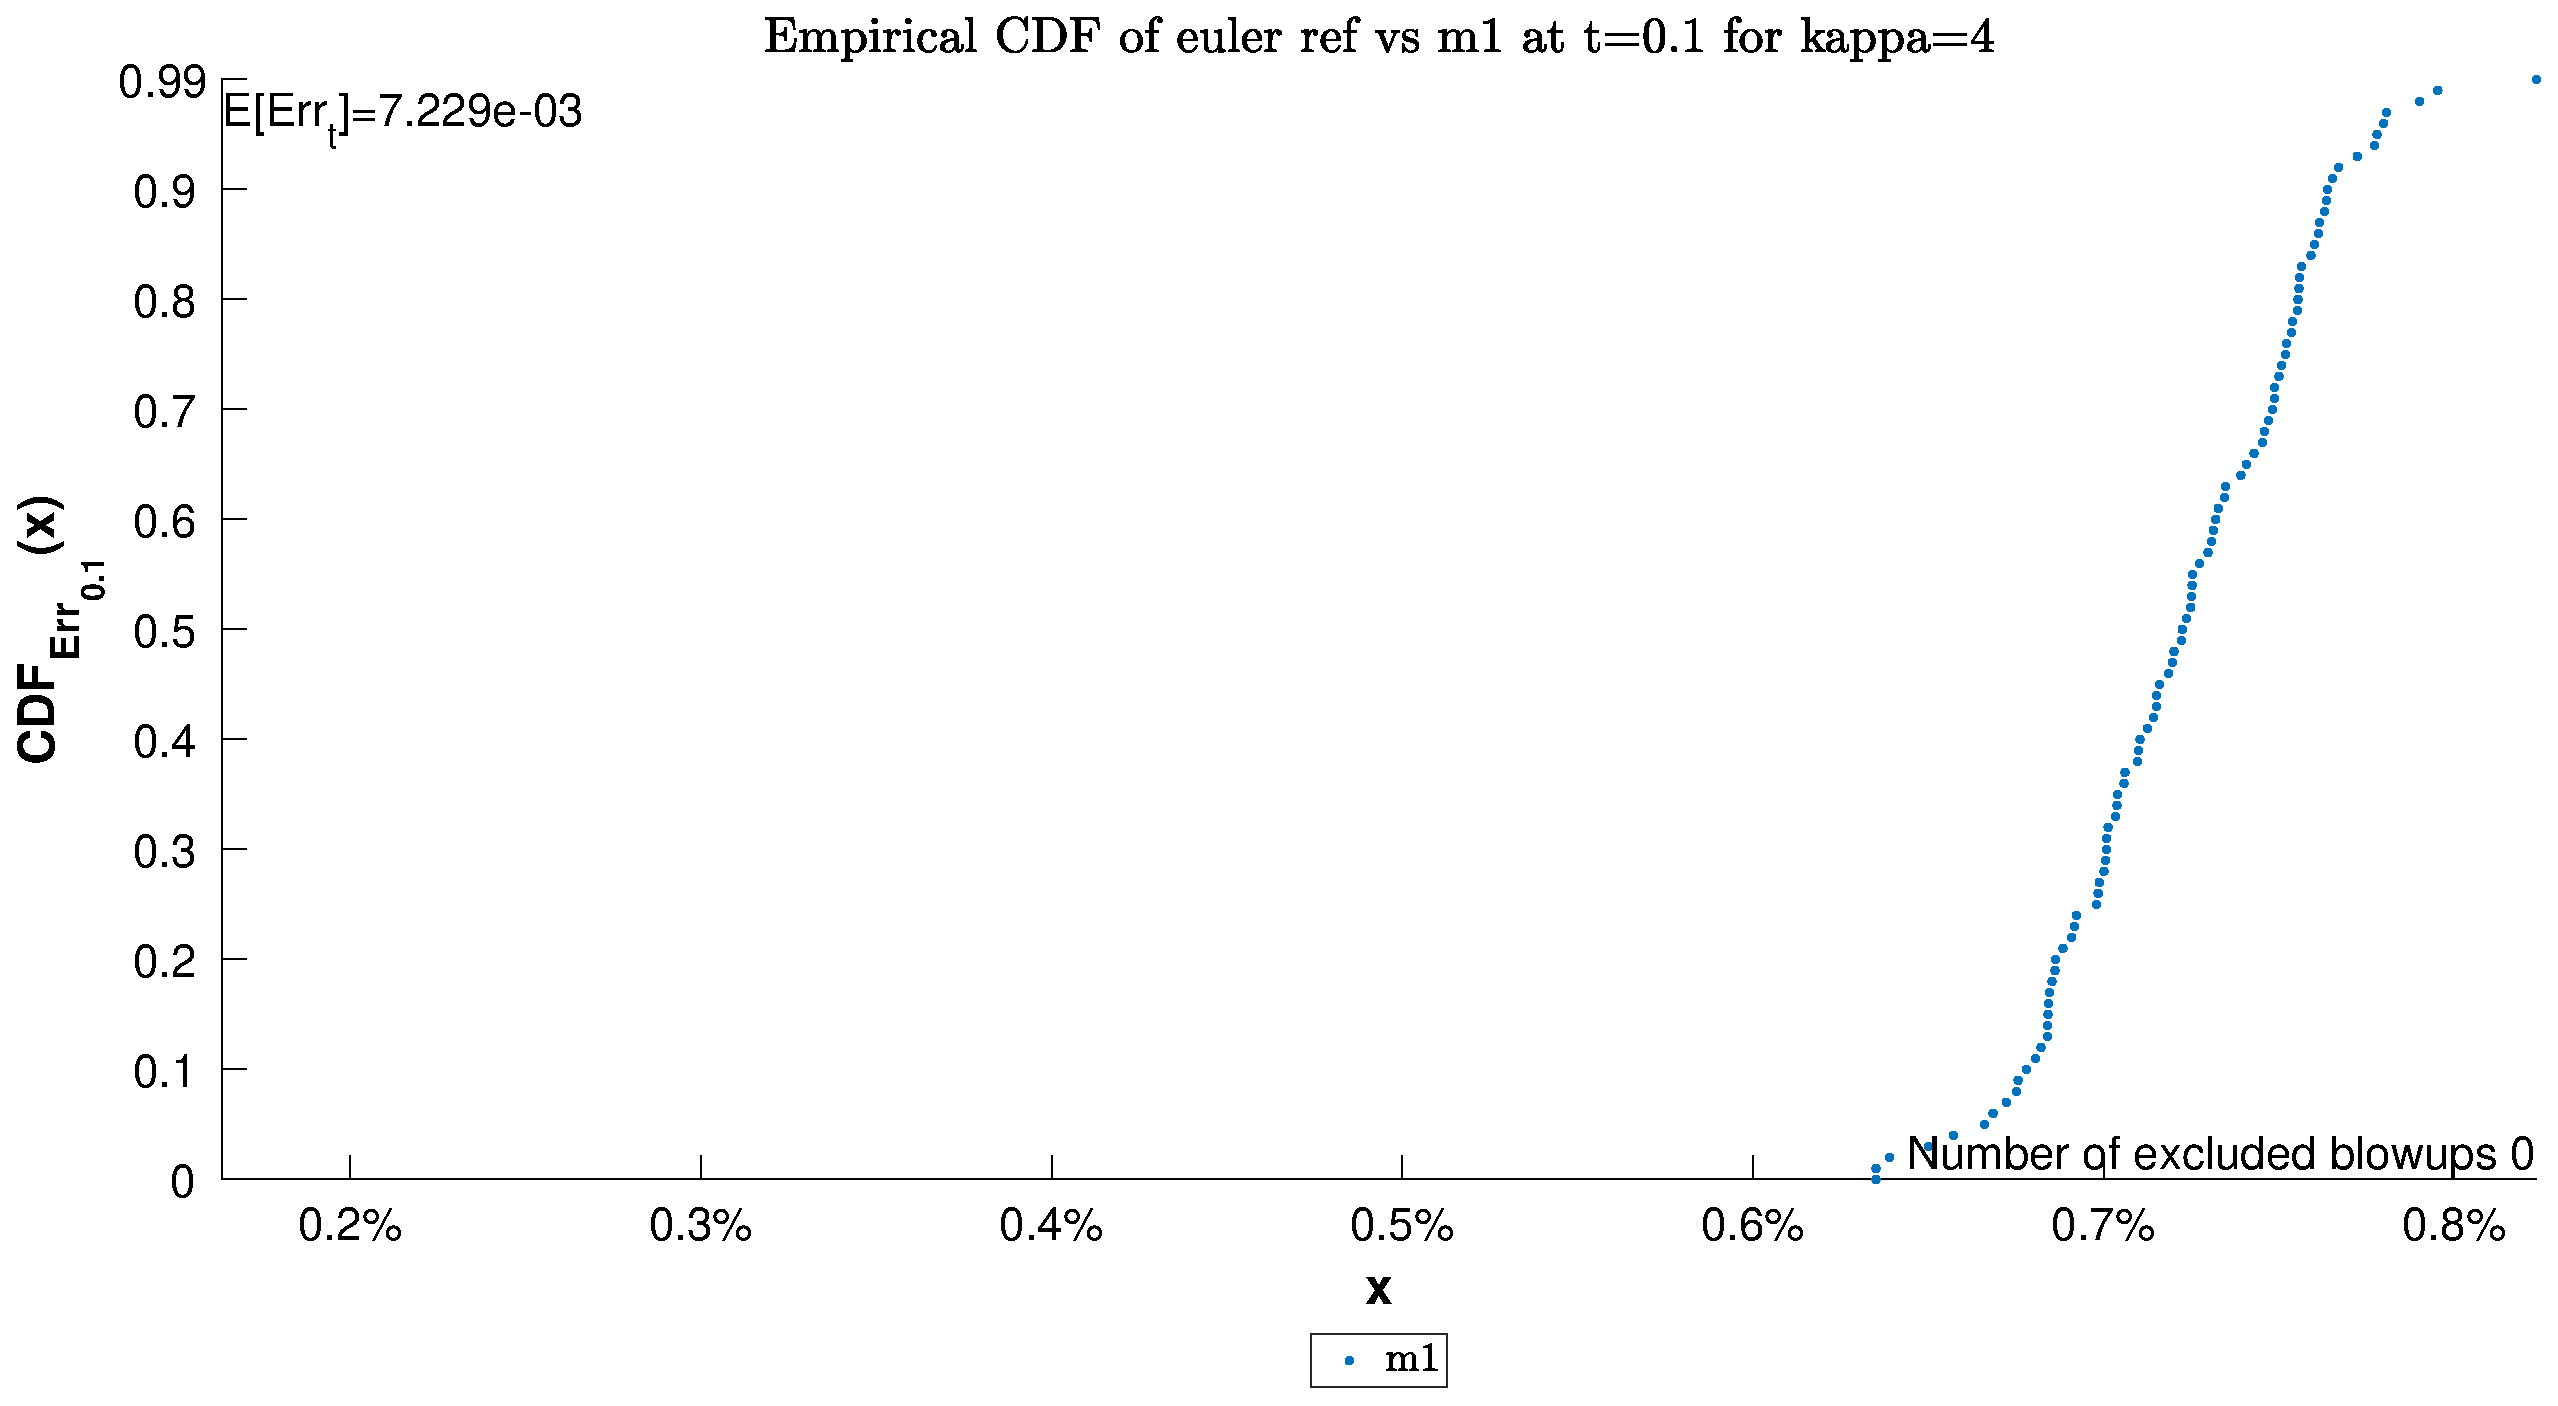
\includegraphics[width=.95\columnwidth]{CDF/CDFEulerRef_18}
\end{landscape}
\begin{landscape}
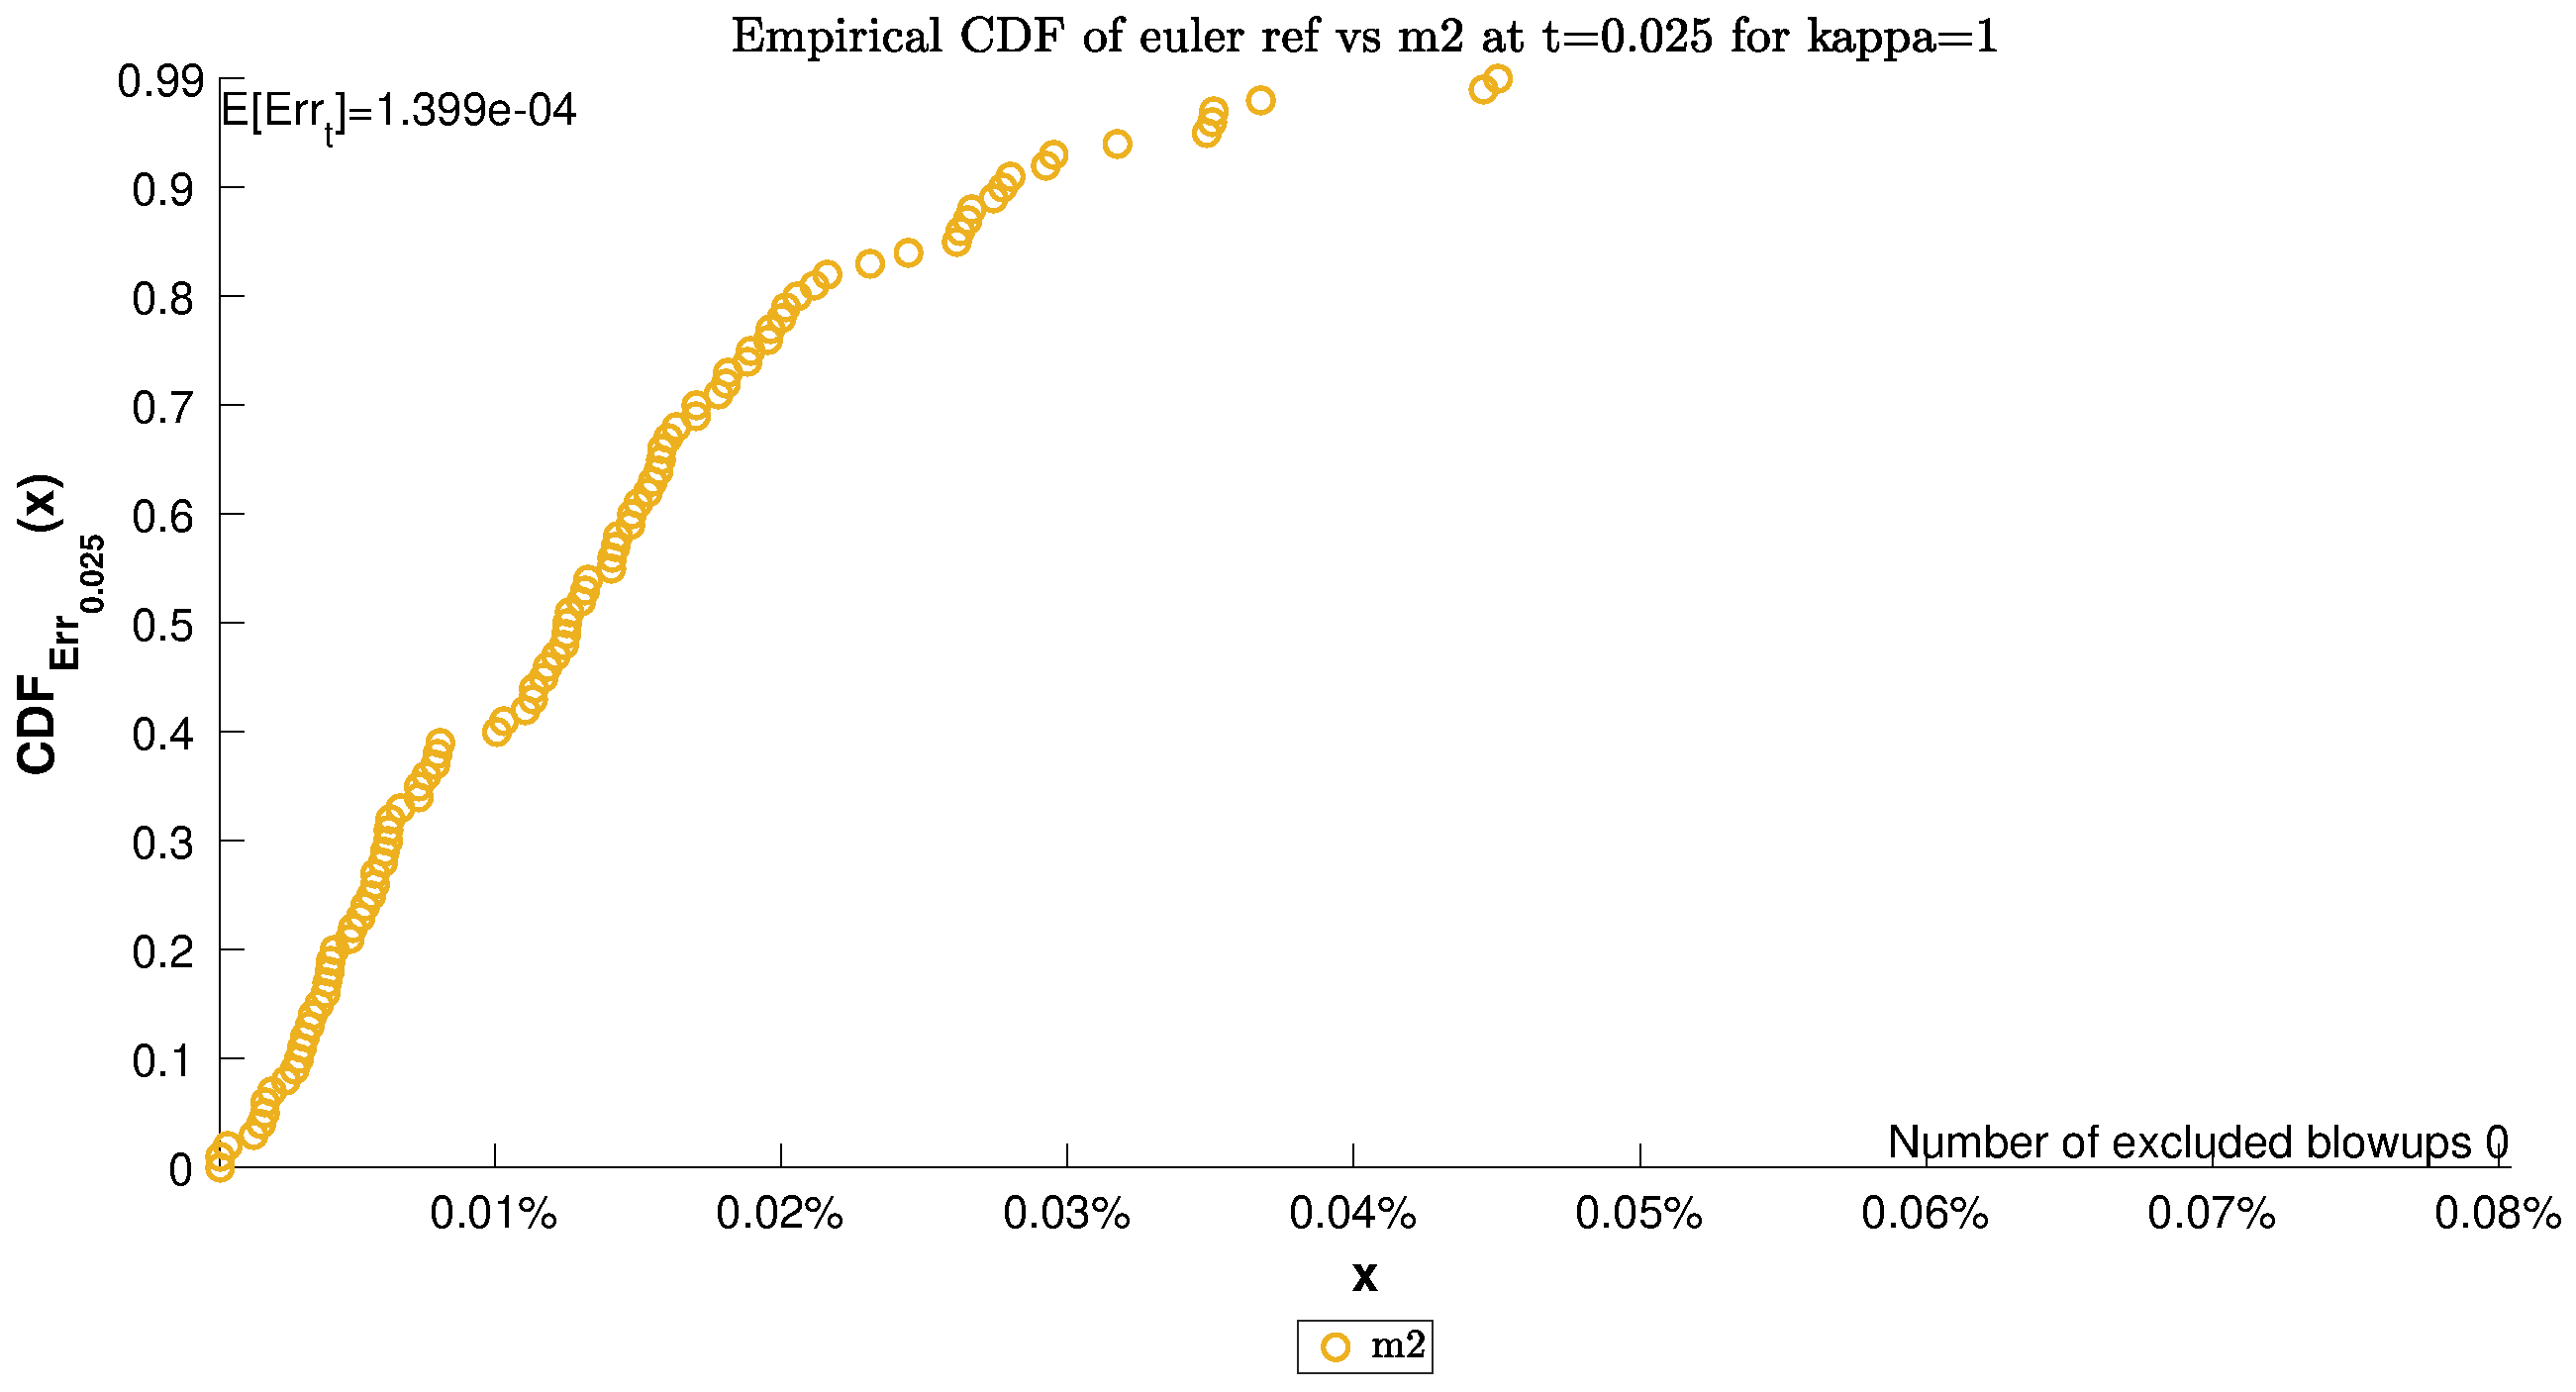
\includegraphics[width=.95\columnwidth]{CDF/CDFEulerRef_19}
\end{landscape}
\begin{landscape}
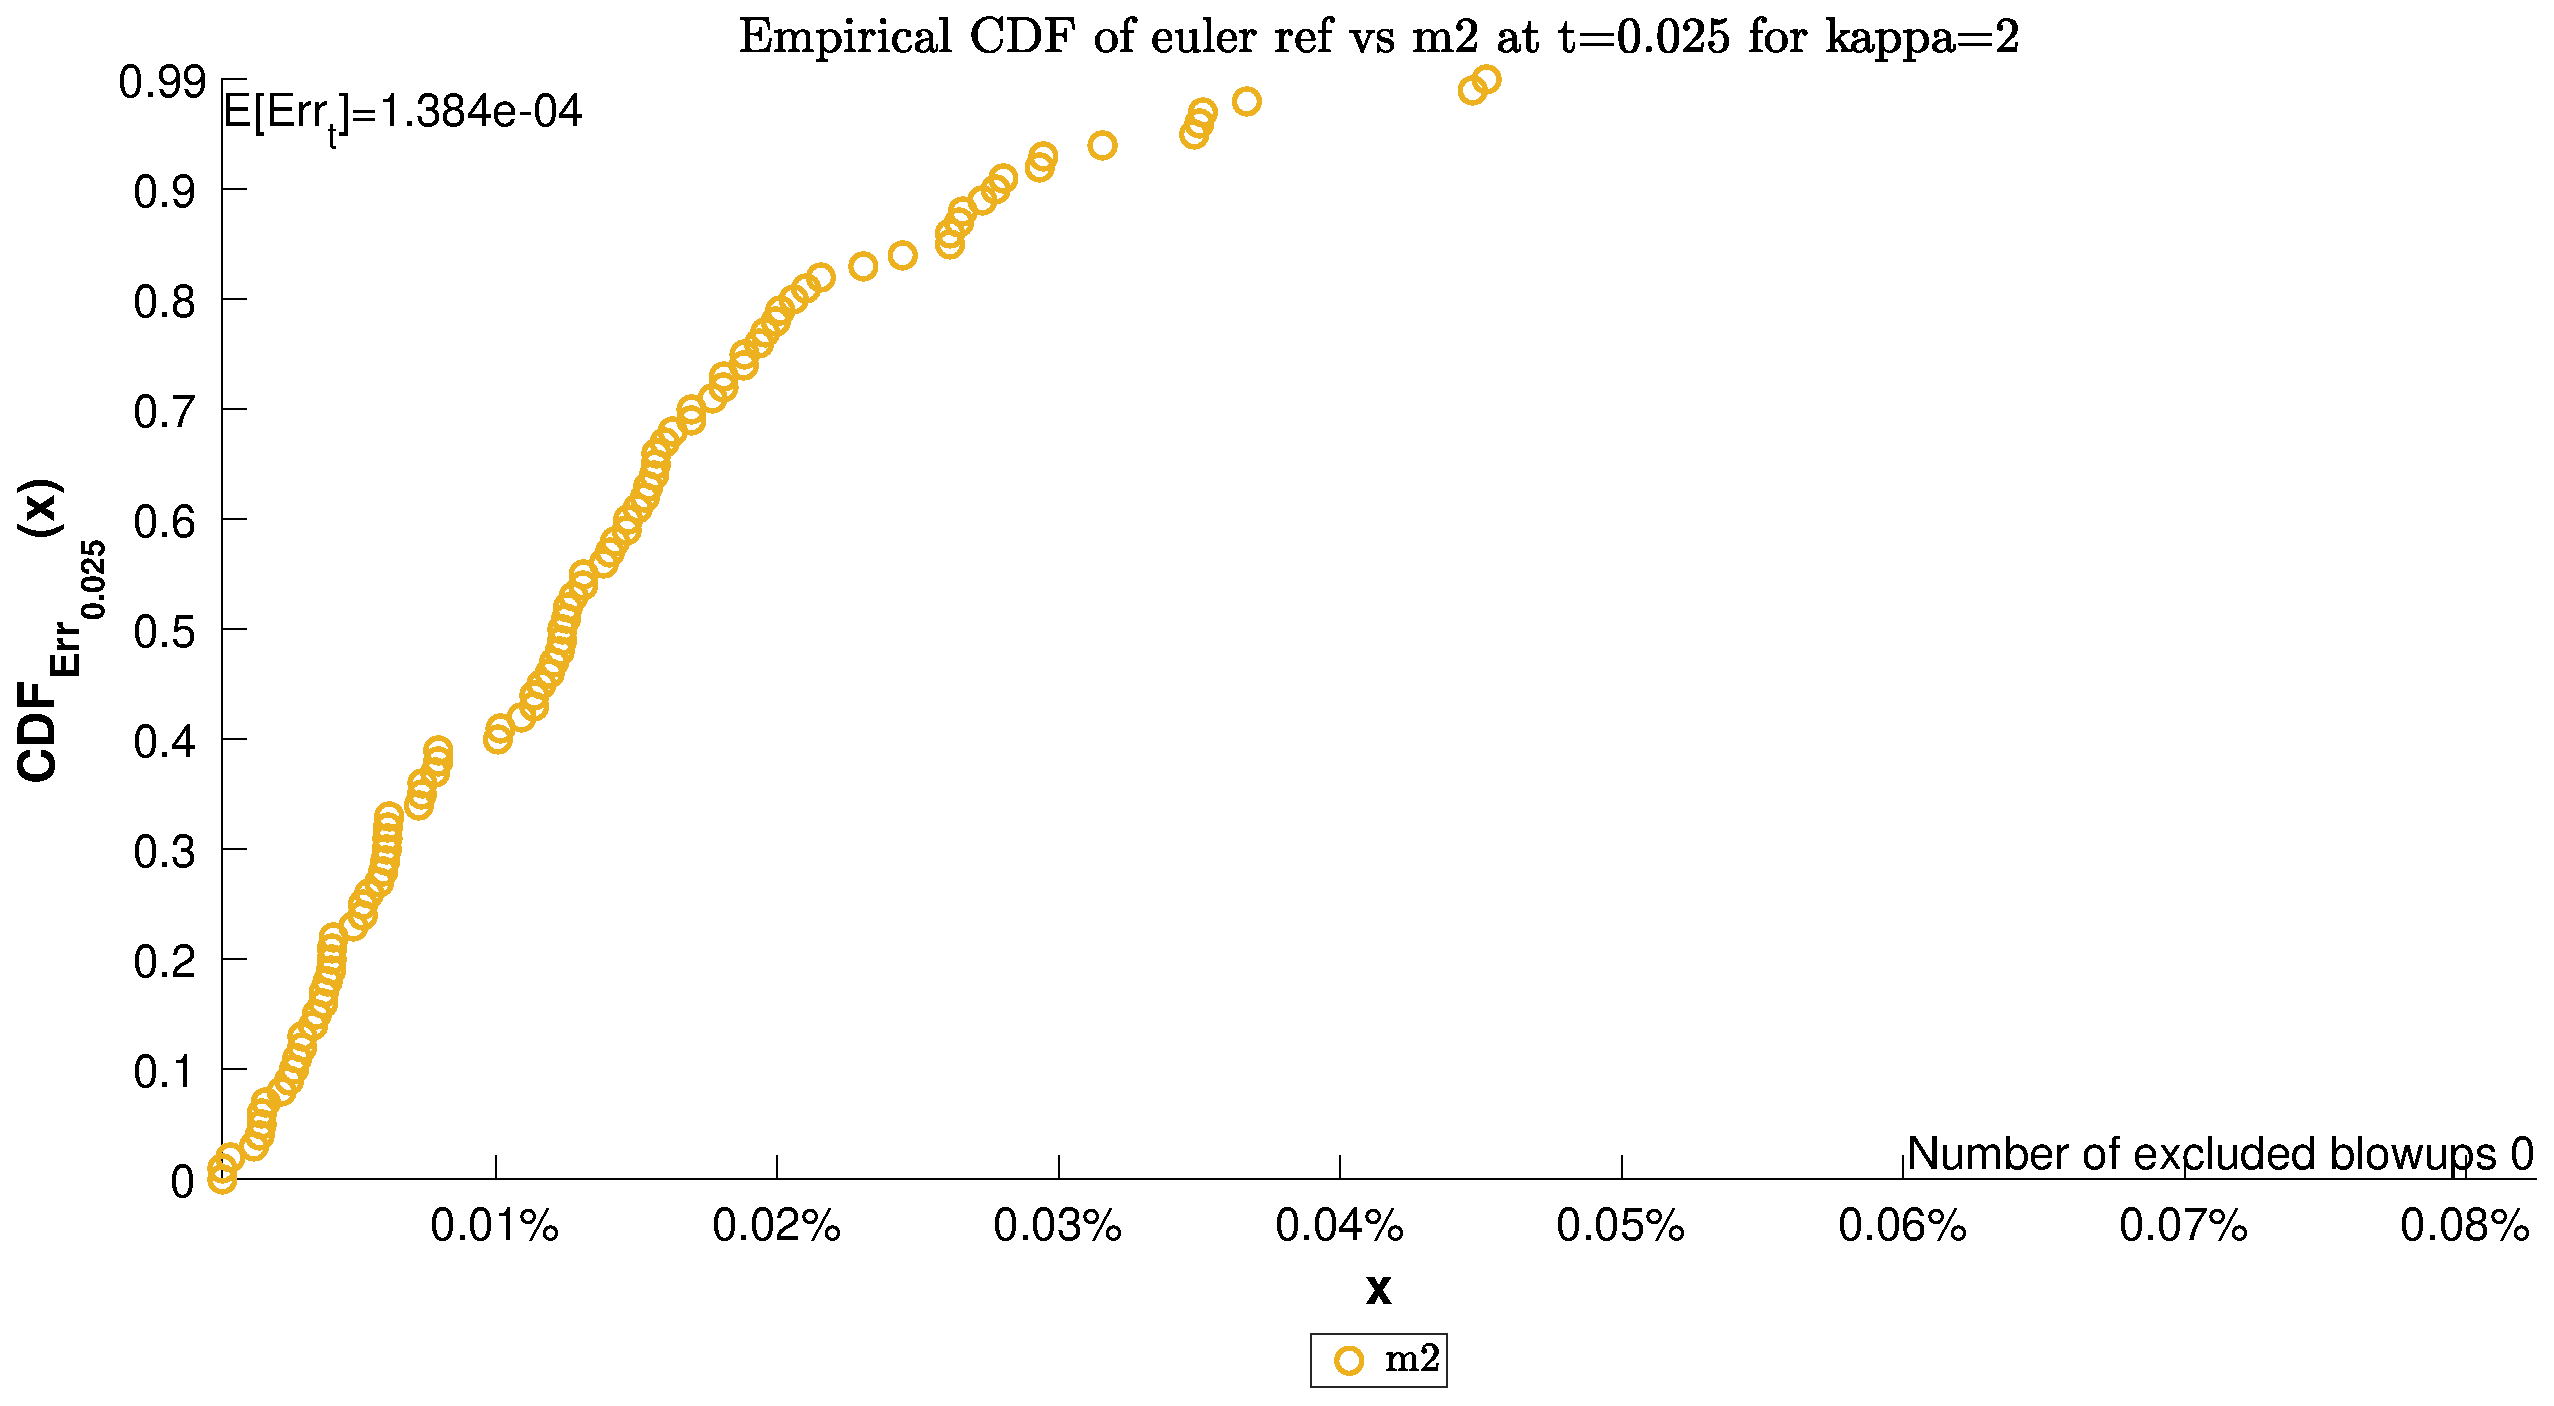
\includegraphics[width=.95\columnwidth]{CDF/CDFEulerRef_20}
\end{landscape}
\begin{landscape}
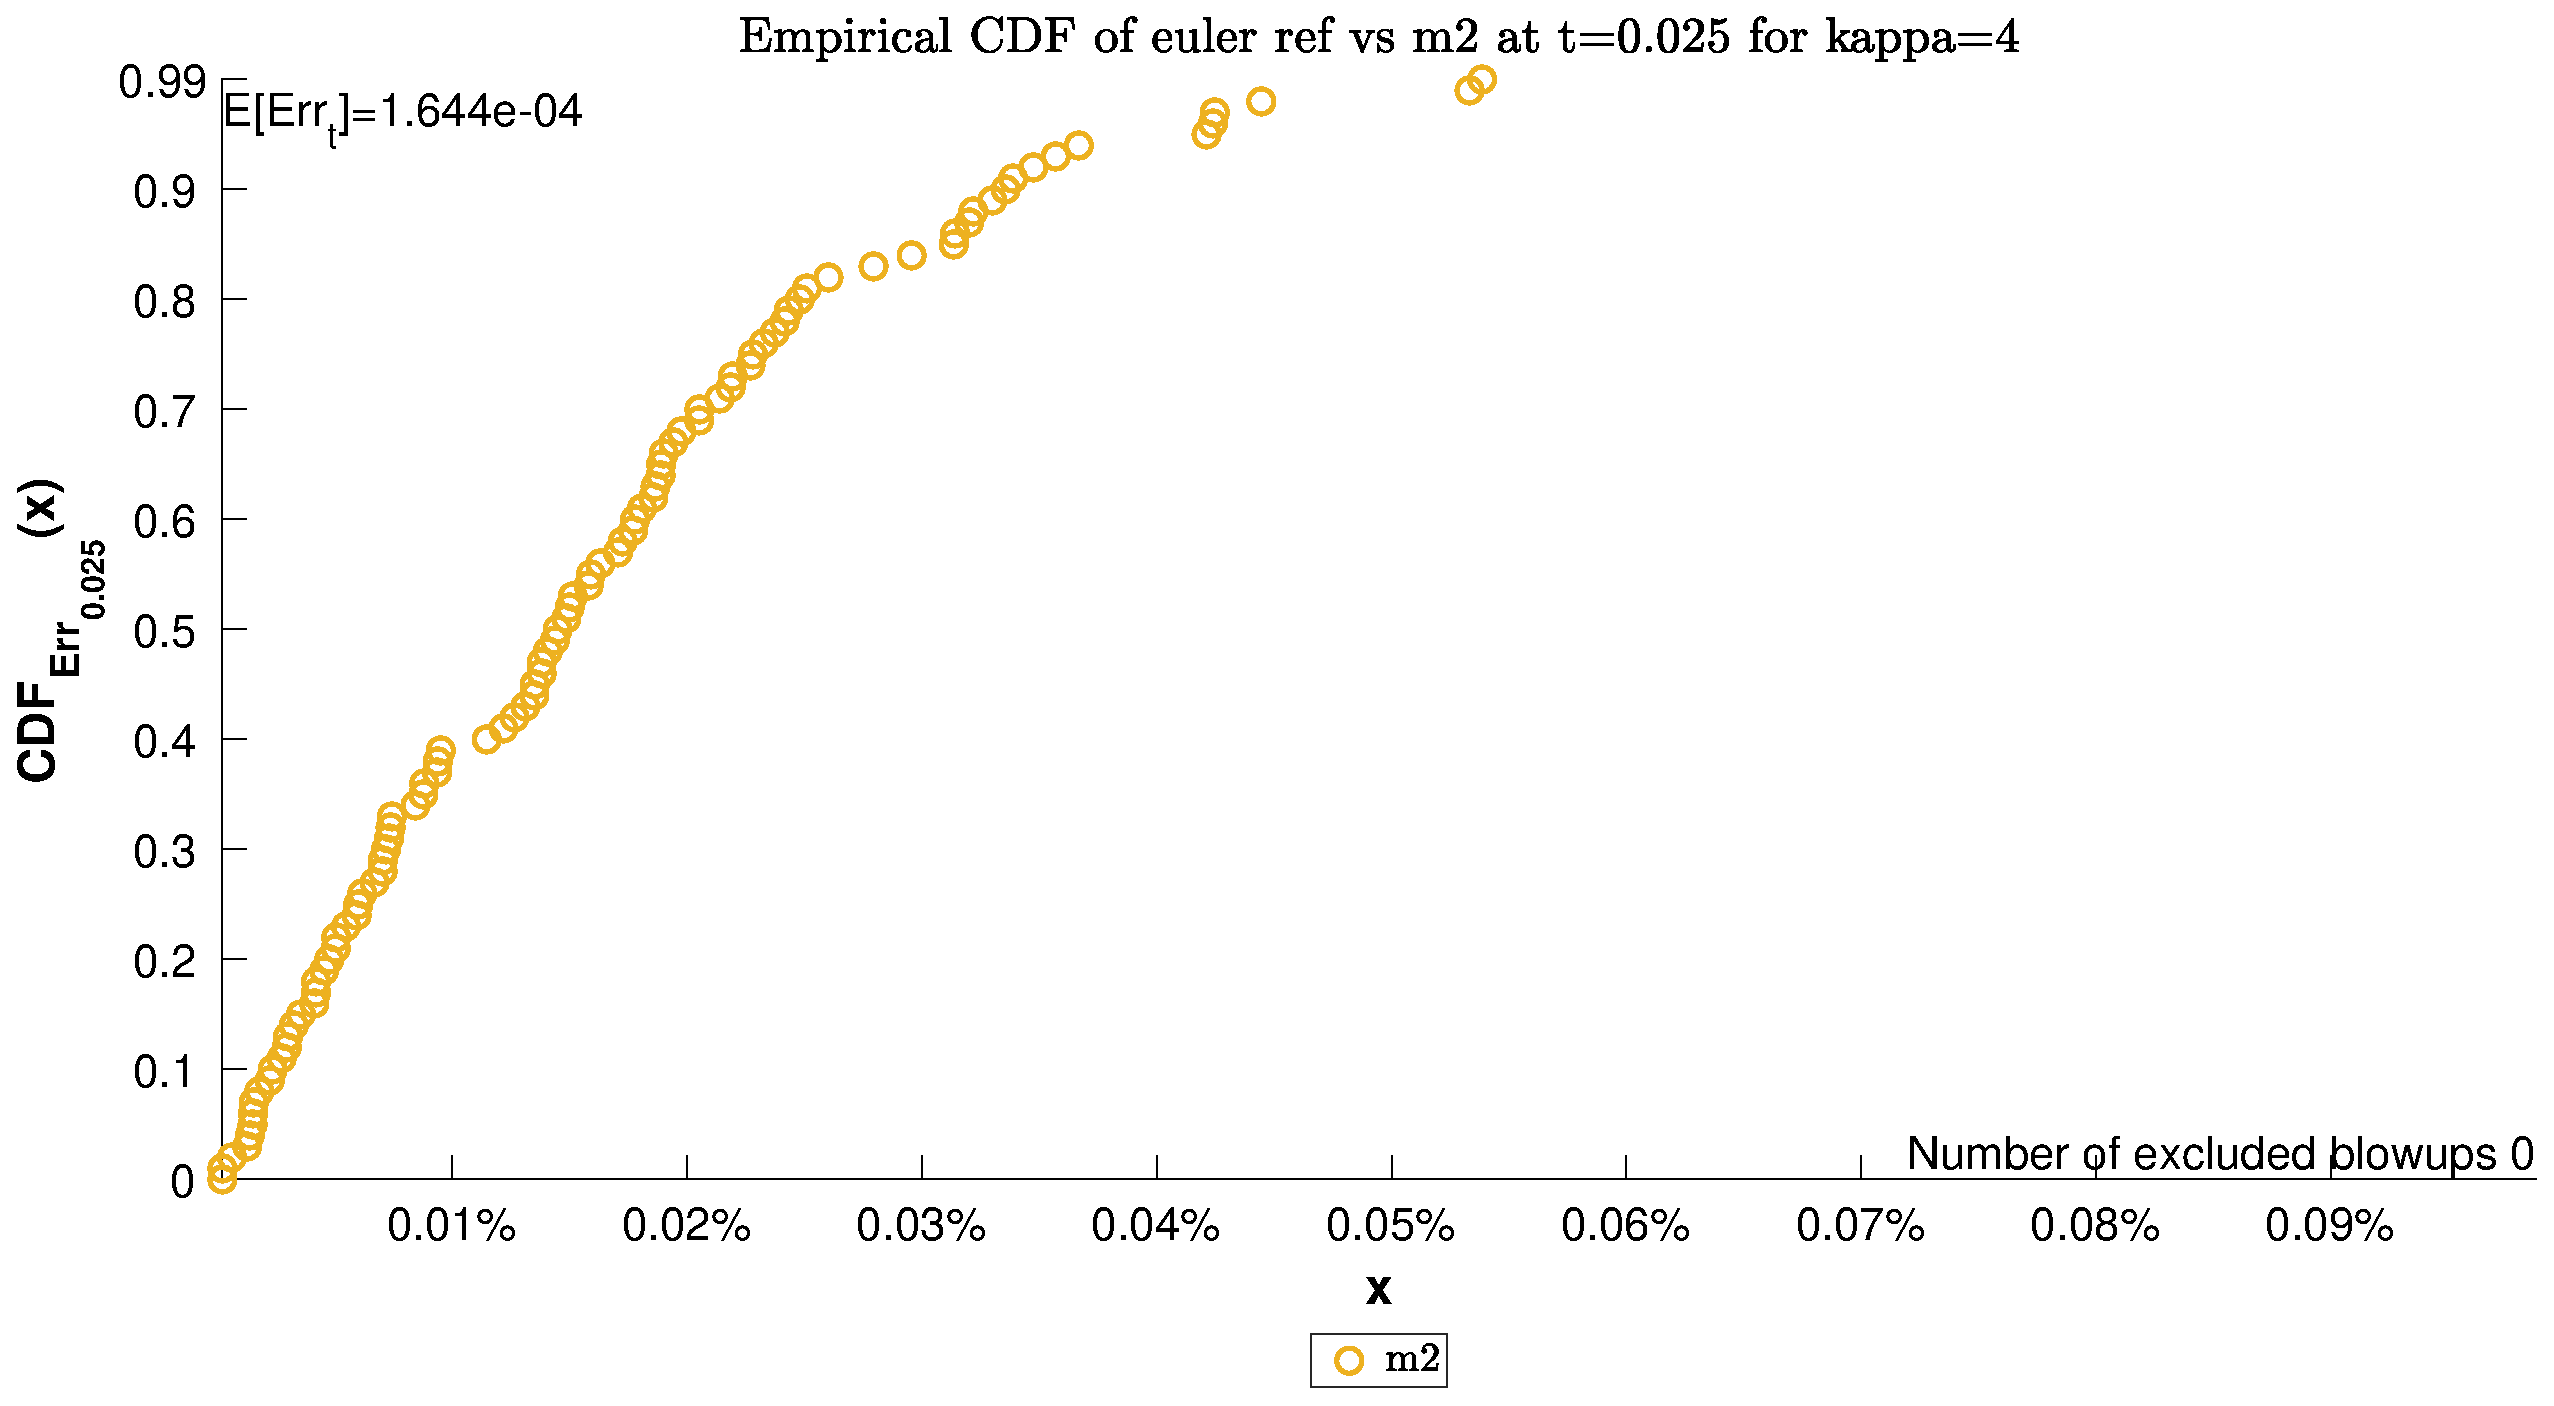
\includegraphics[width=.95\columnwidth]{CDF/CDFEulerRef_21}
\end{landscape}
\begin{landscape}
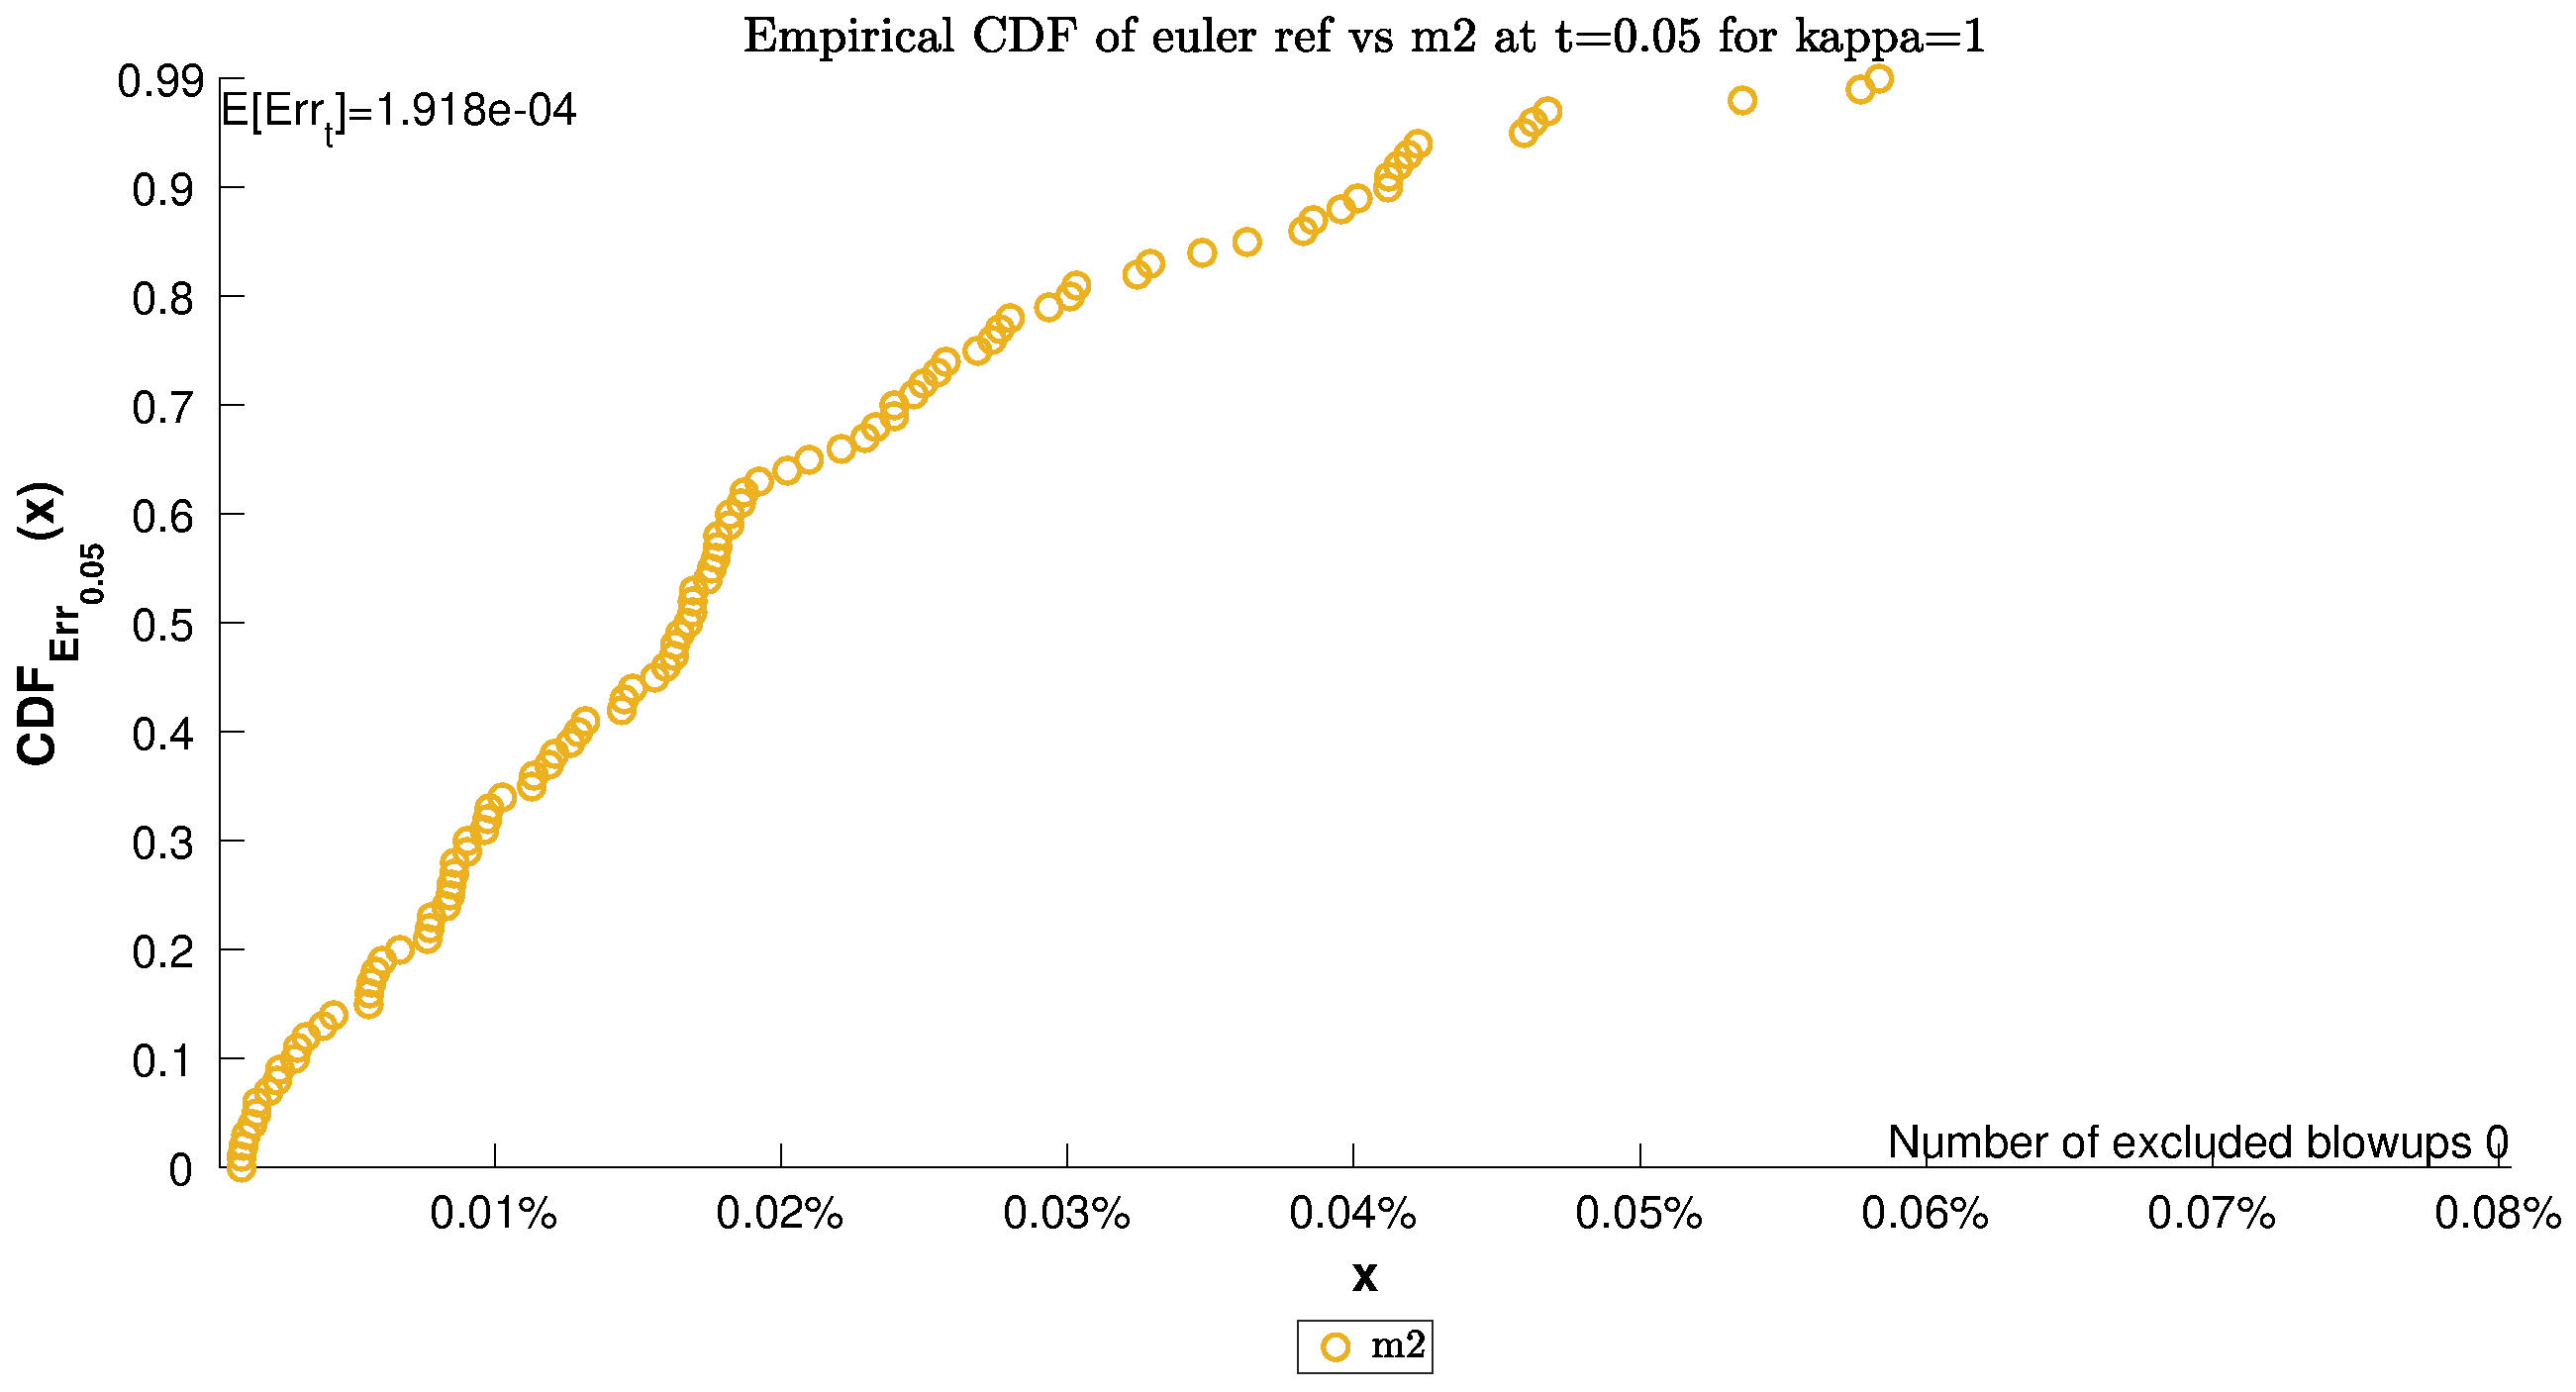
\includegraphics[width=.95\columnwidth]{CDF/CDFEulerRef_22}
\end{landscape}
\begin{landscape}
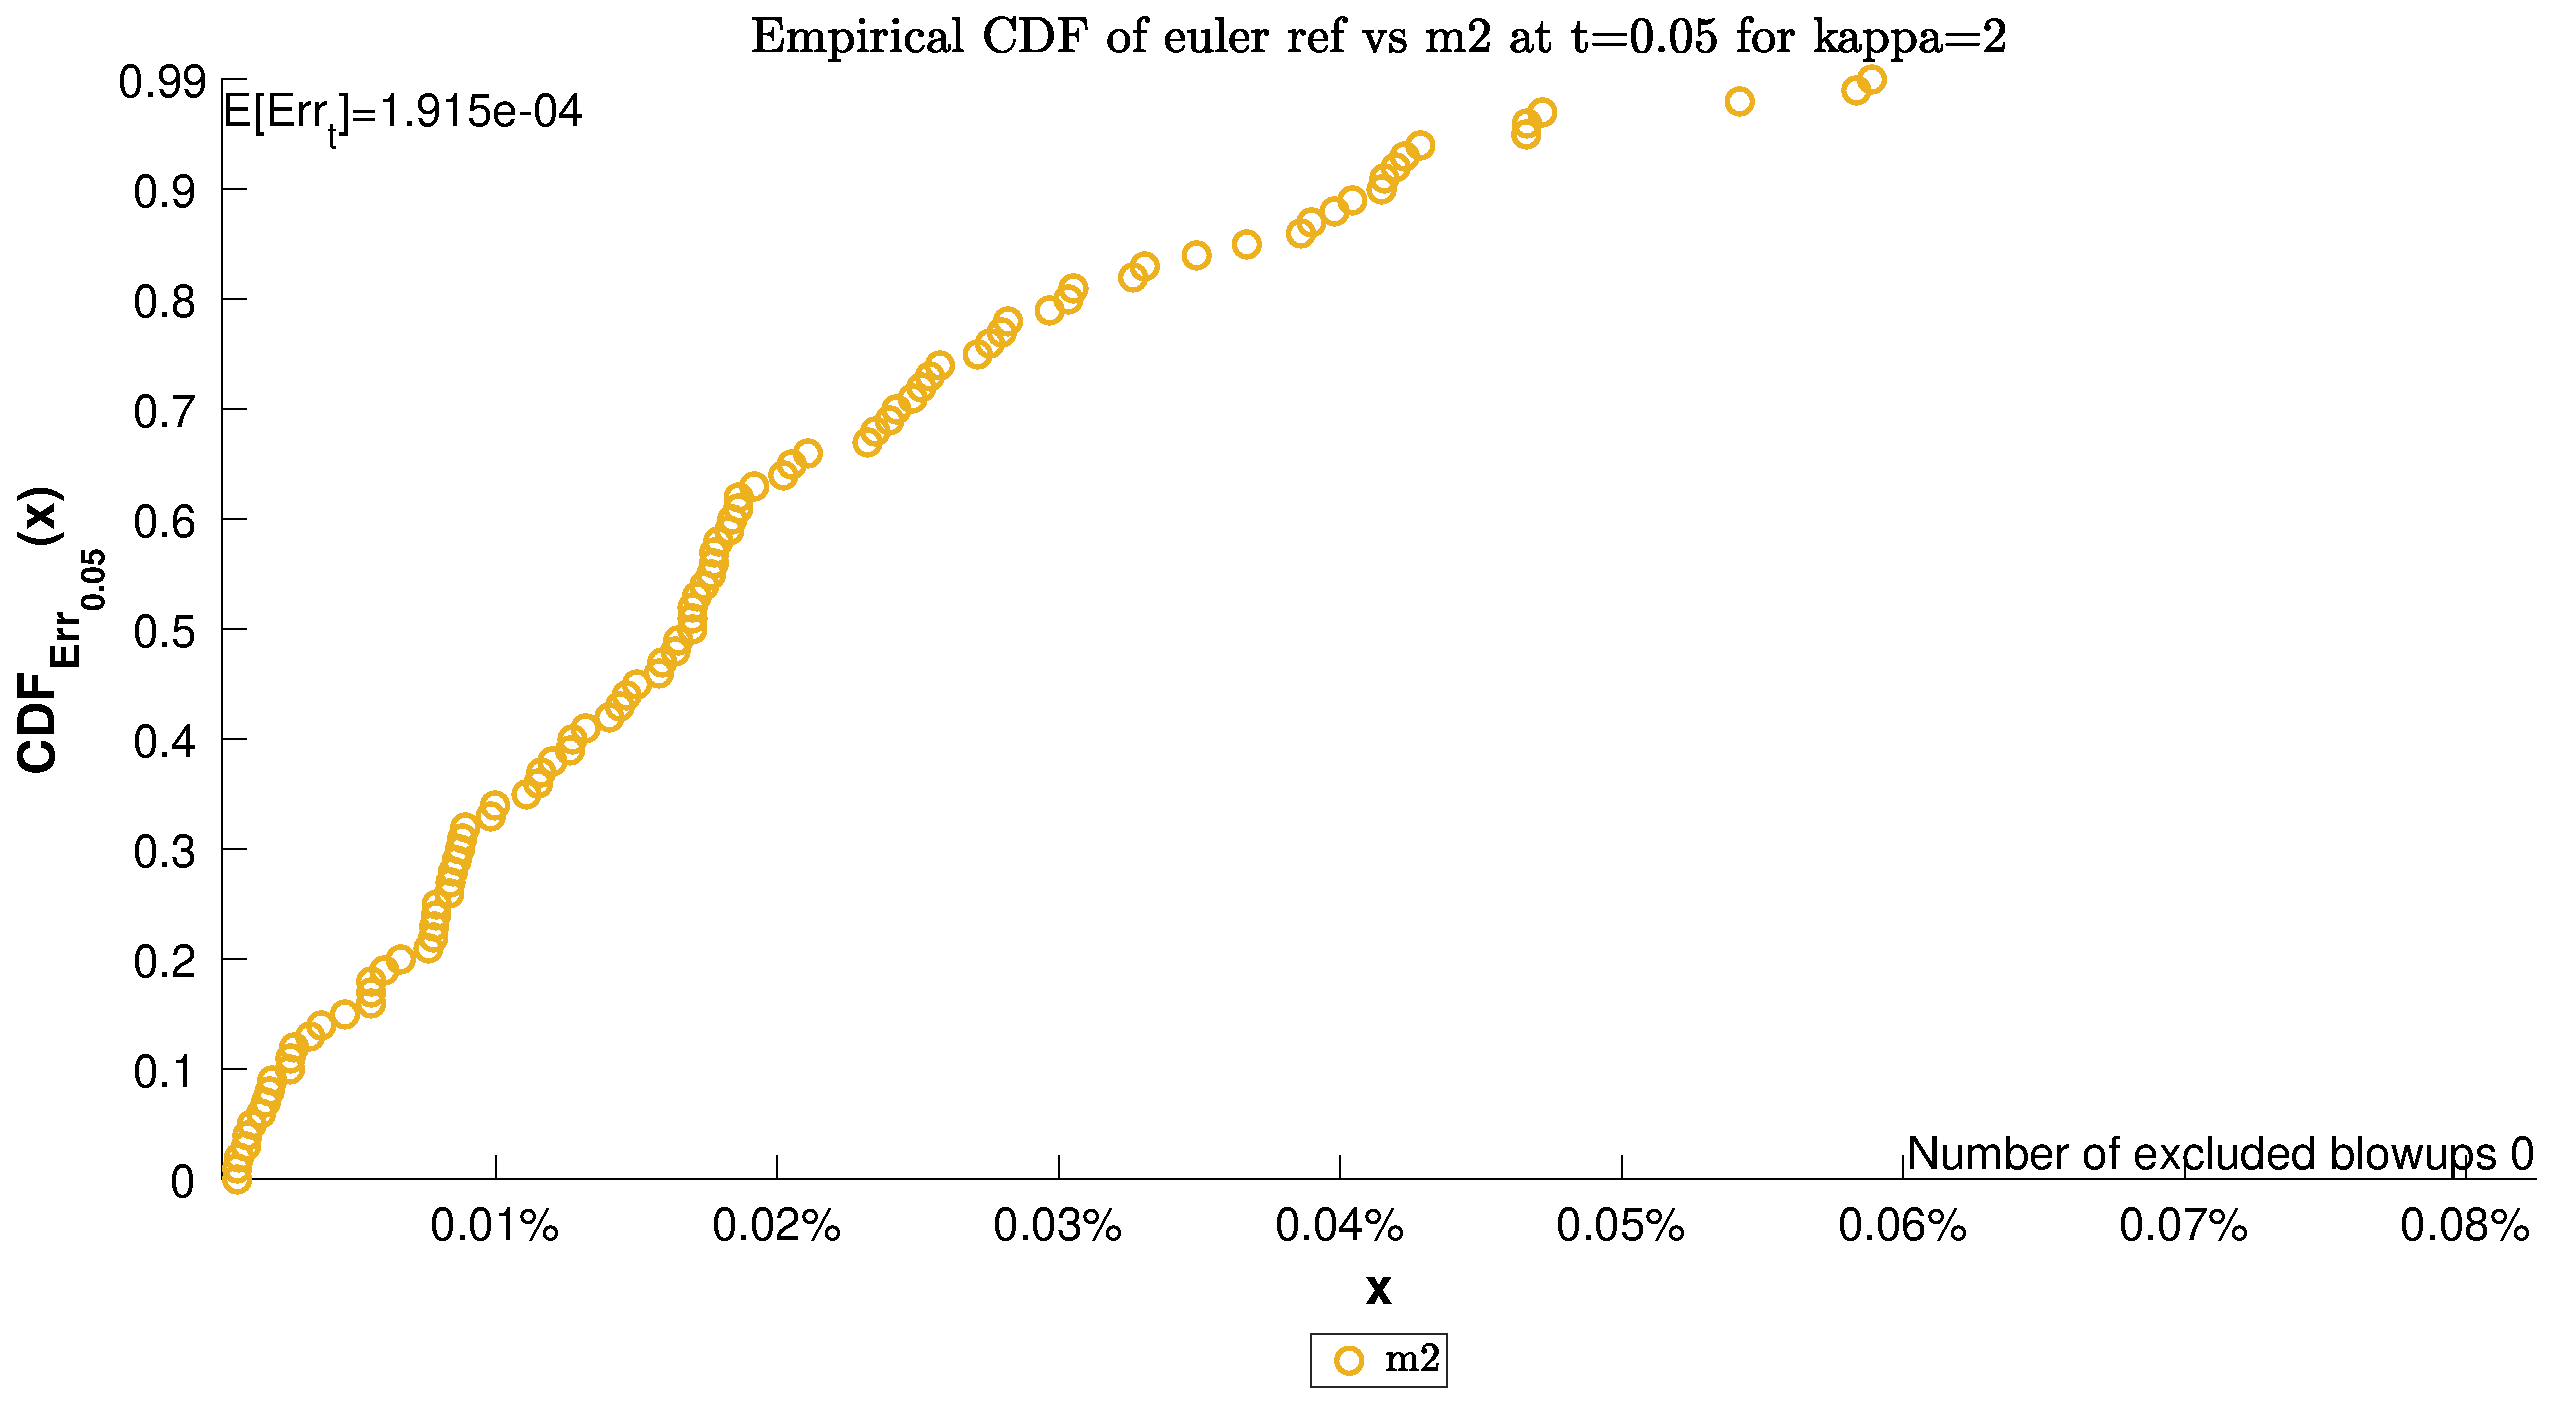
\includegraphics[width=.95\columnwidth]{CDF/CDFEulerRef_23}
\end{landscape}
\begin{landscape}
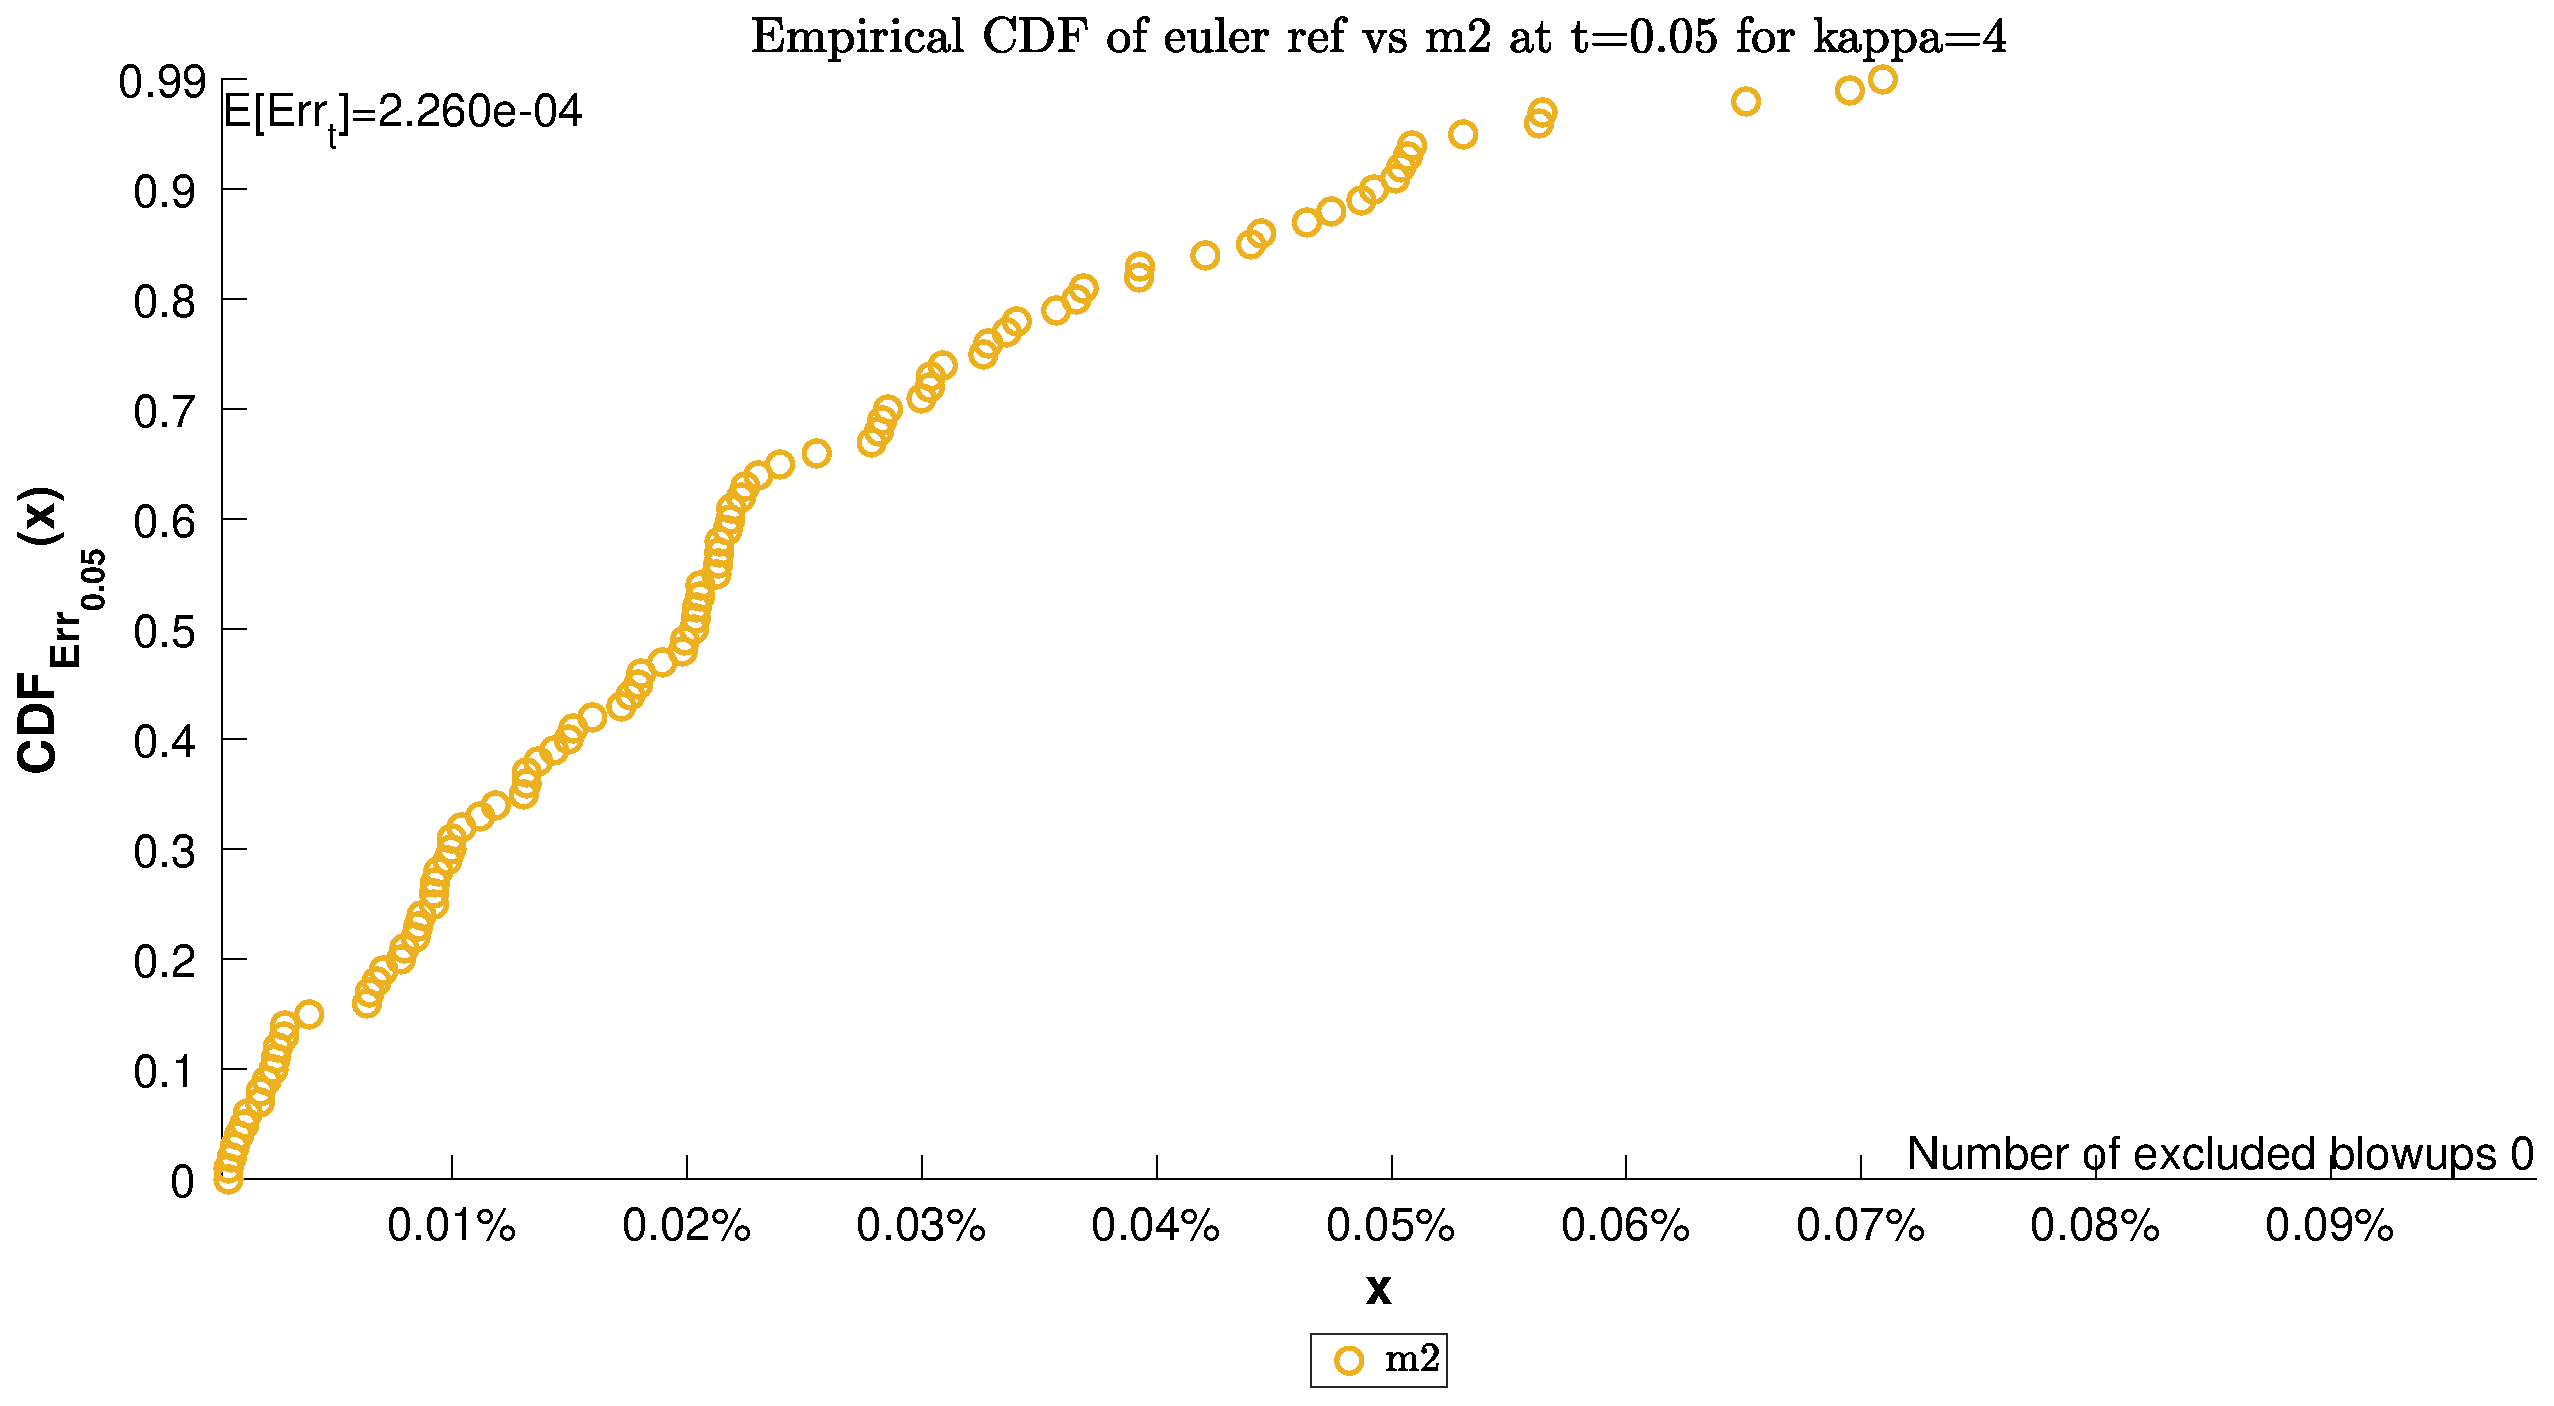
\includegraphics[width=.95\columnwidth]{CDF/CDFEulerRef_24}
\end{landscape}
\begin{landscape}
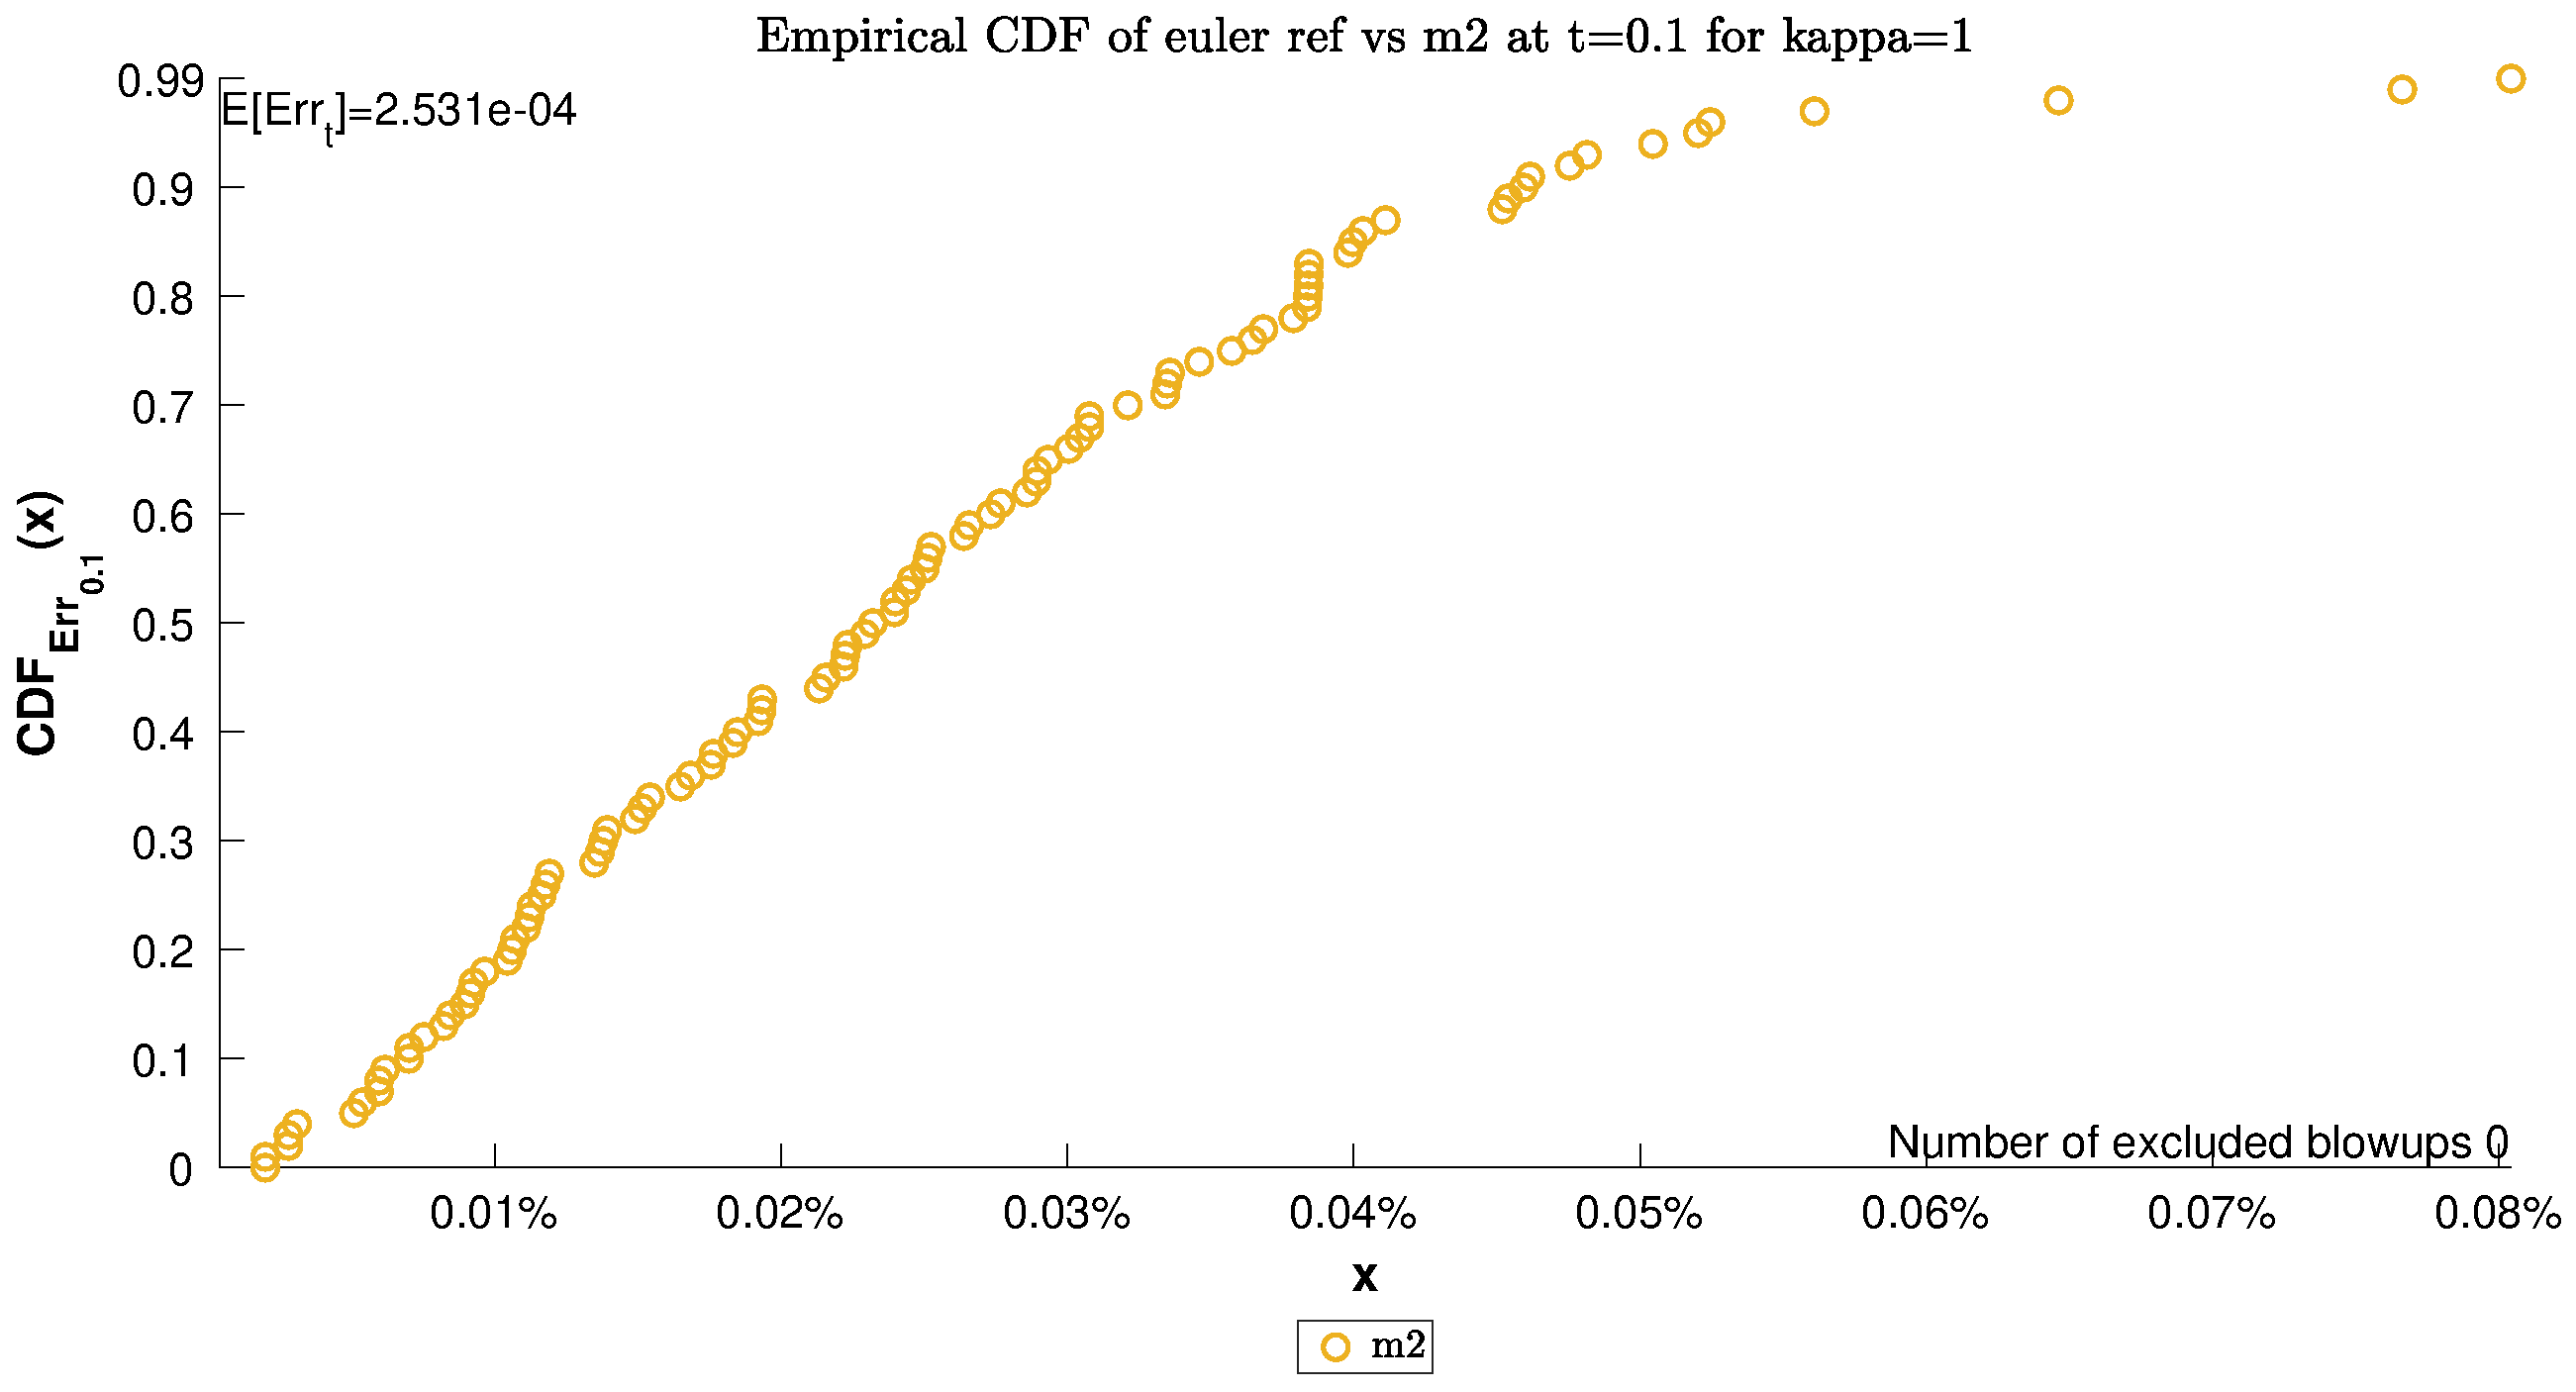
\includegraphics[width=.95\columnwidth]{CDF/CDFEulerRef_25}
\end{landscape}
\begin{landscape}
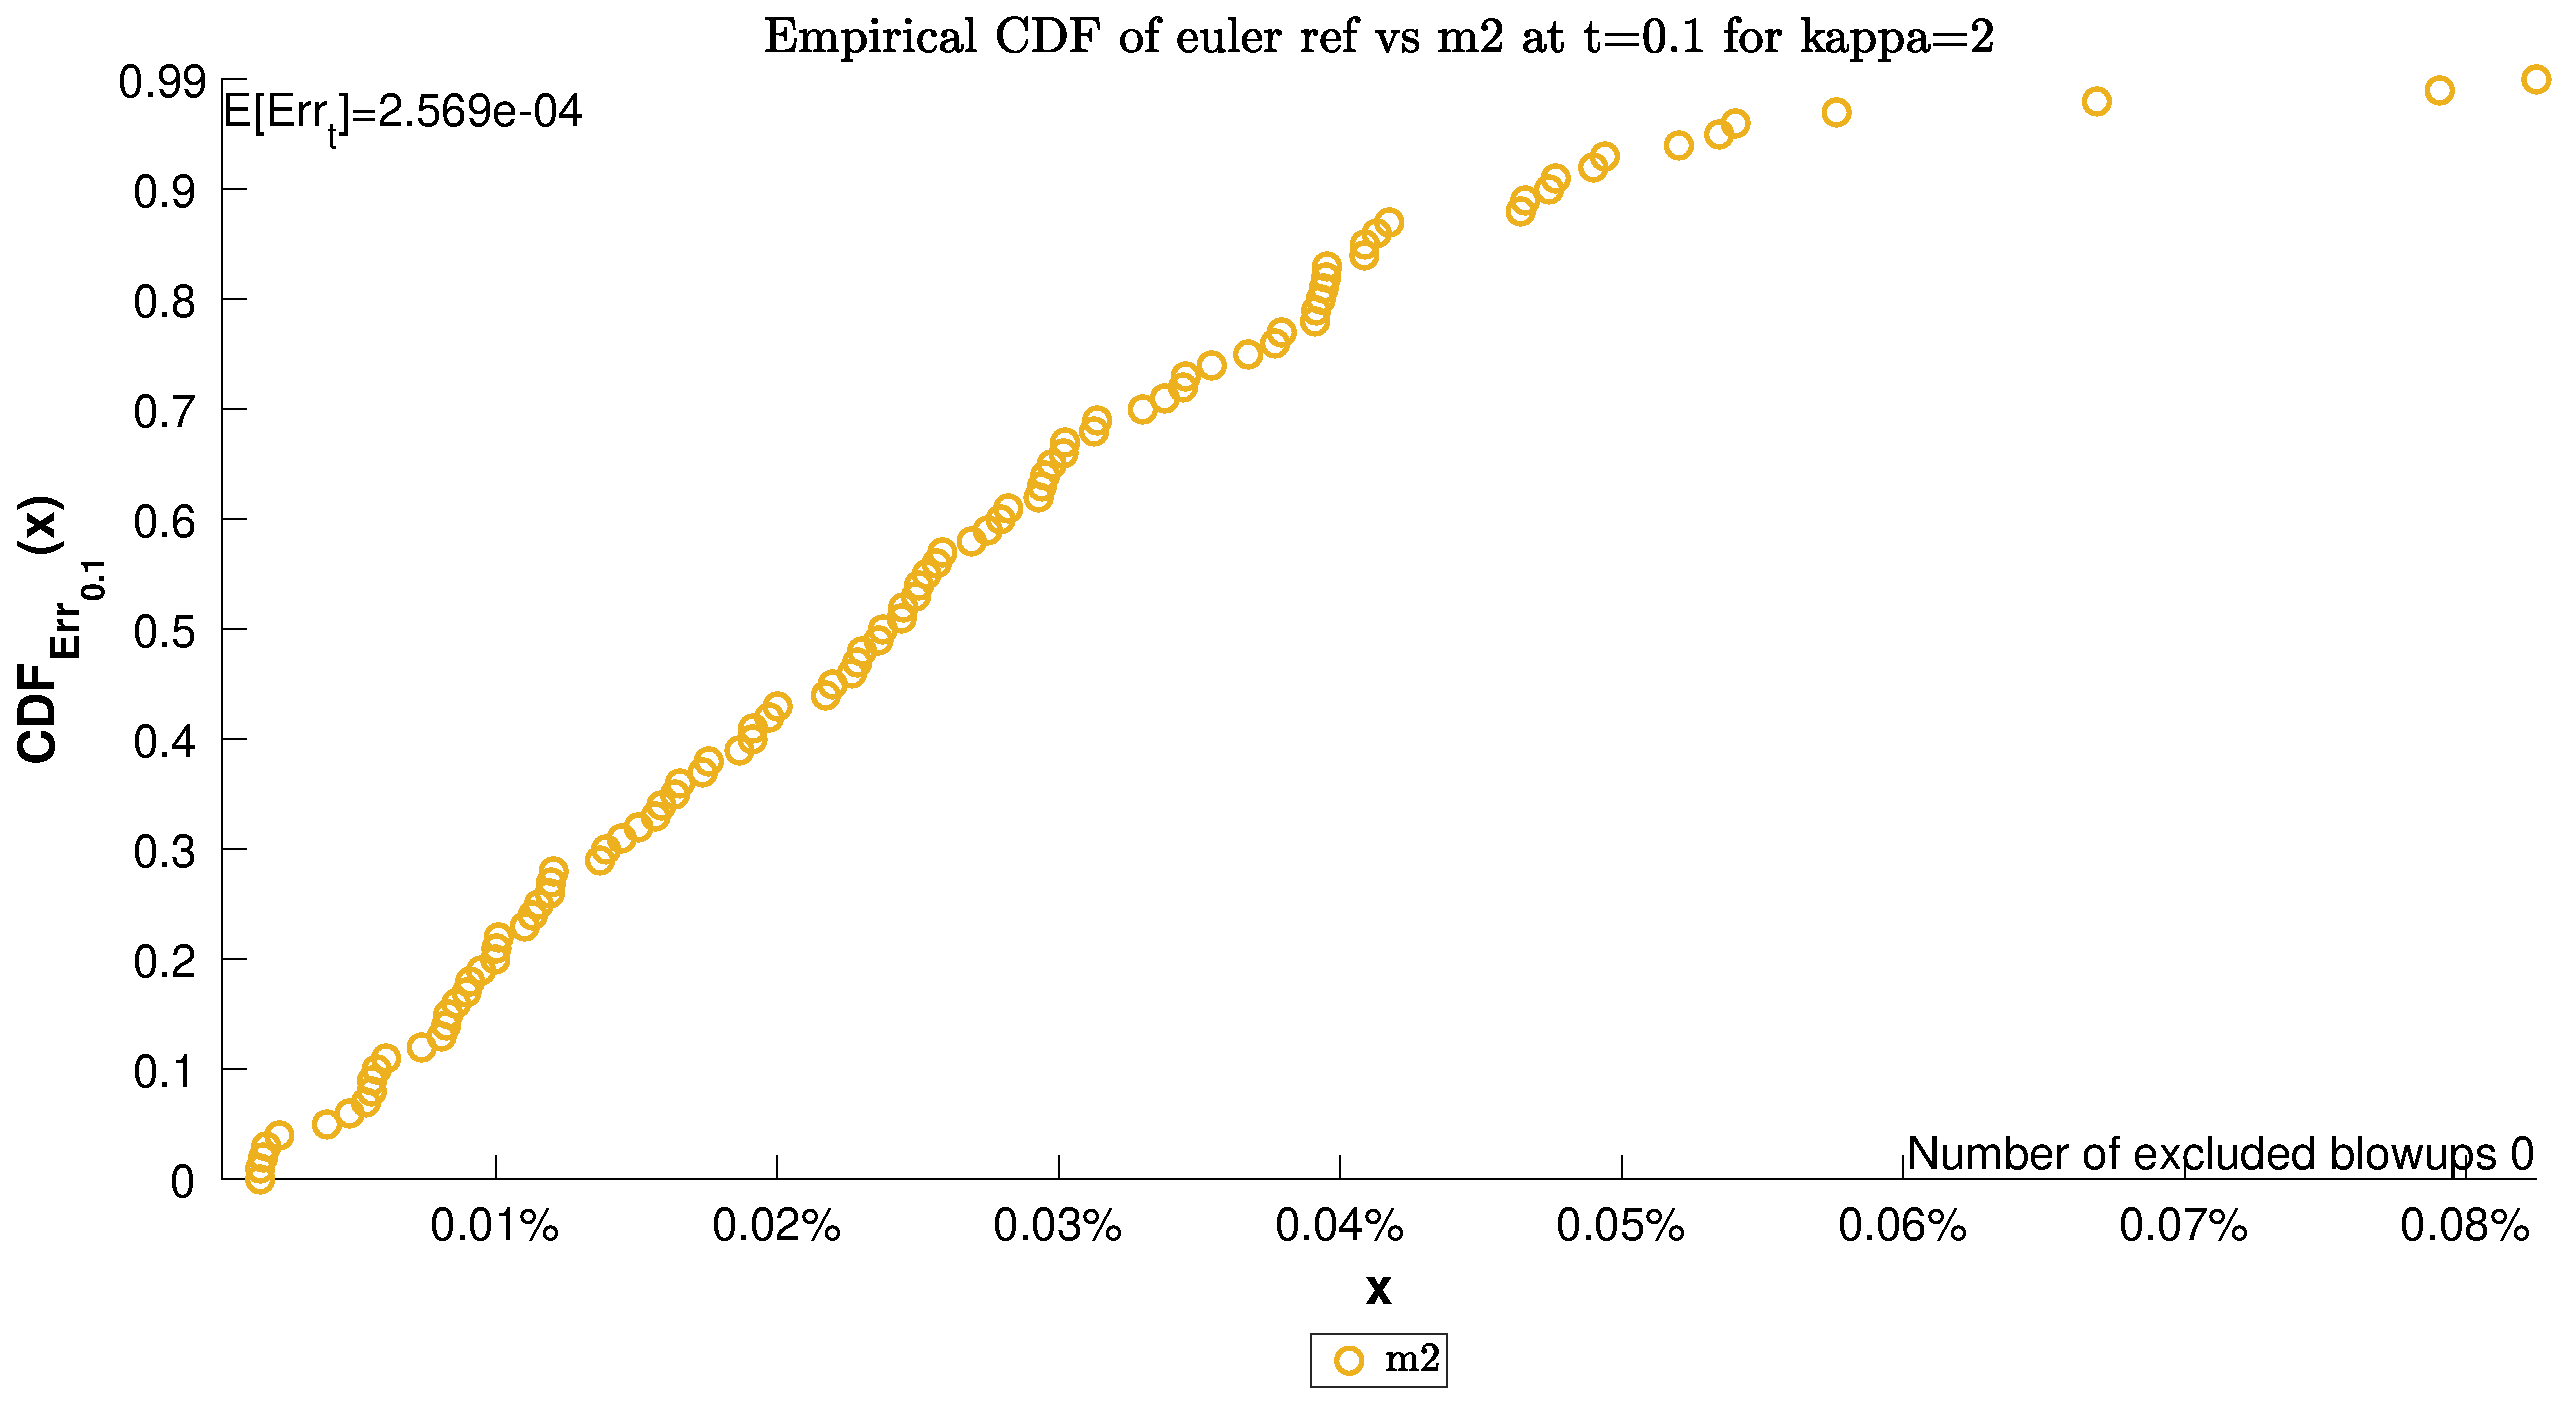
\includegraphics[width=.95\columnwidth]{CDF/CDFEulerRef_26}
\end{landscape}
\begin{landscape}
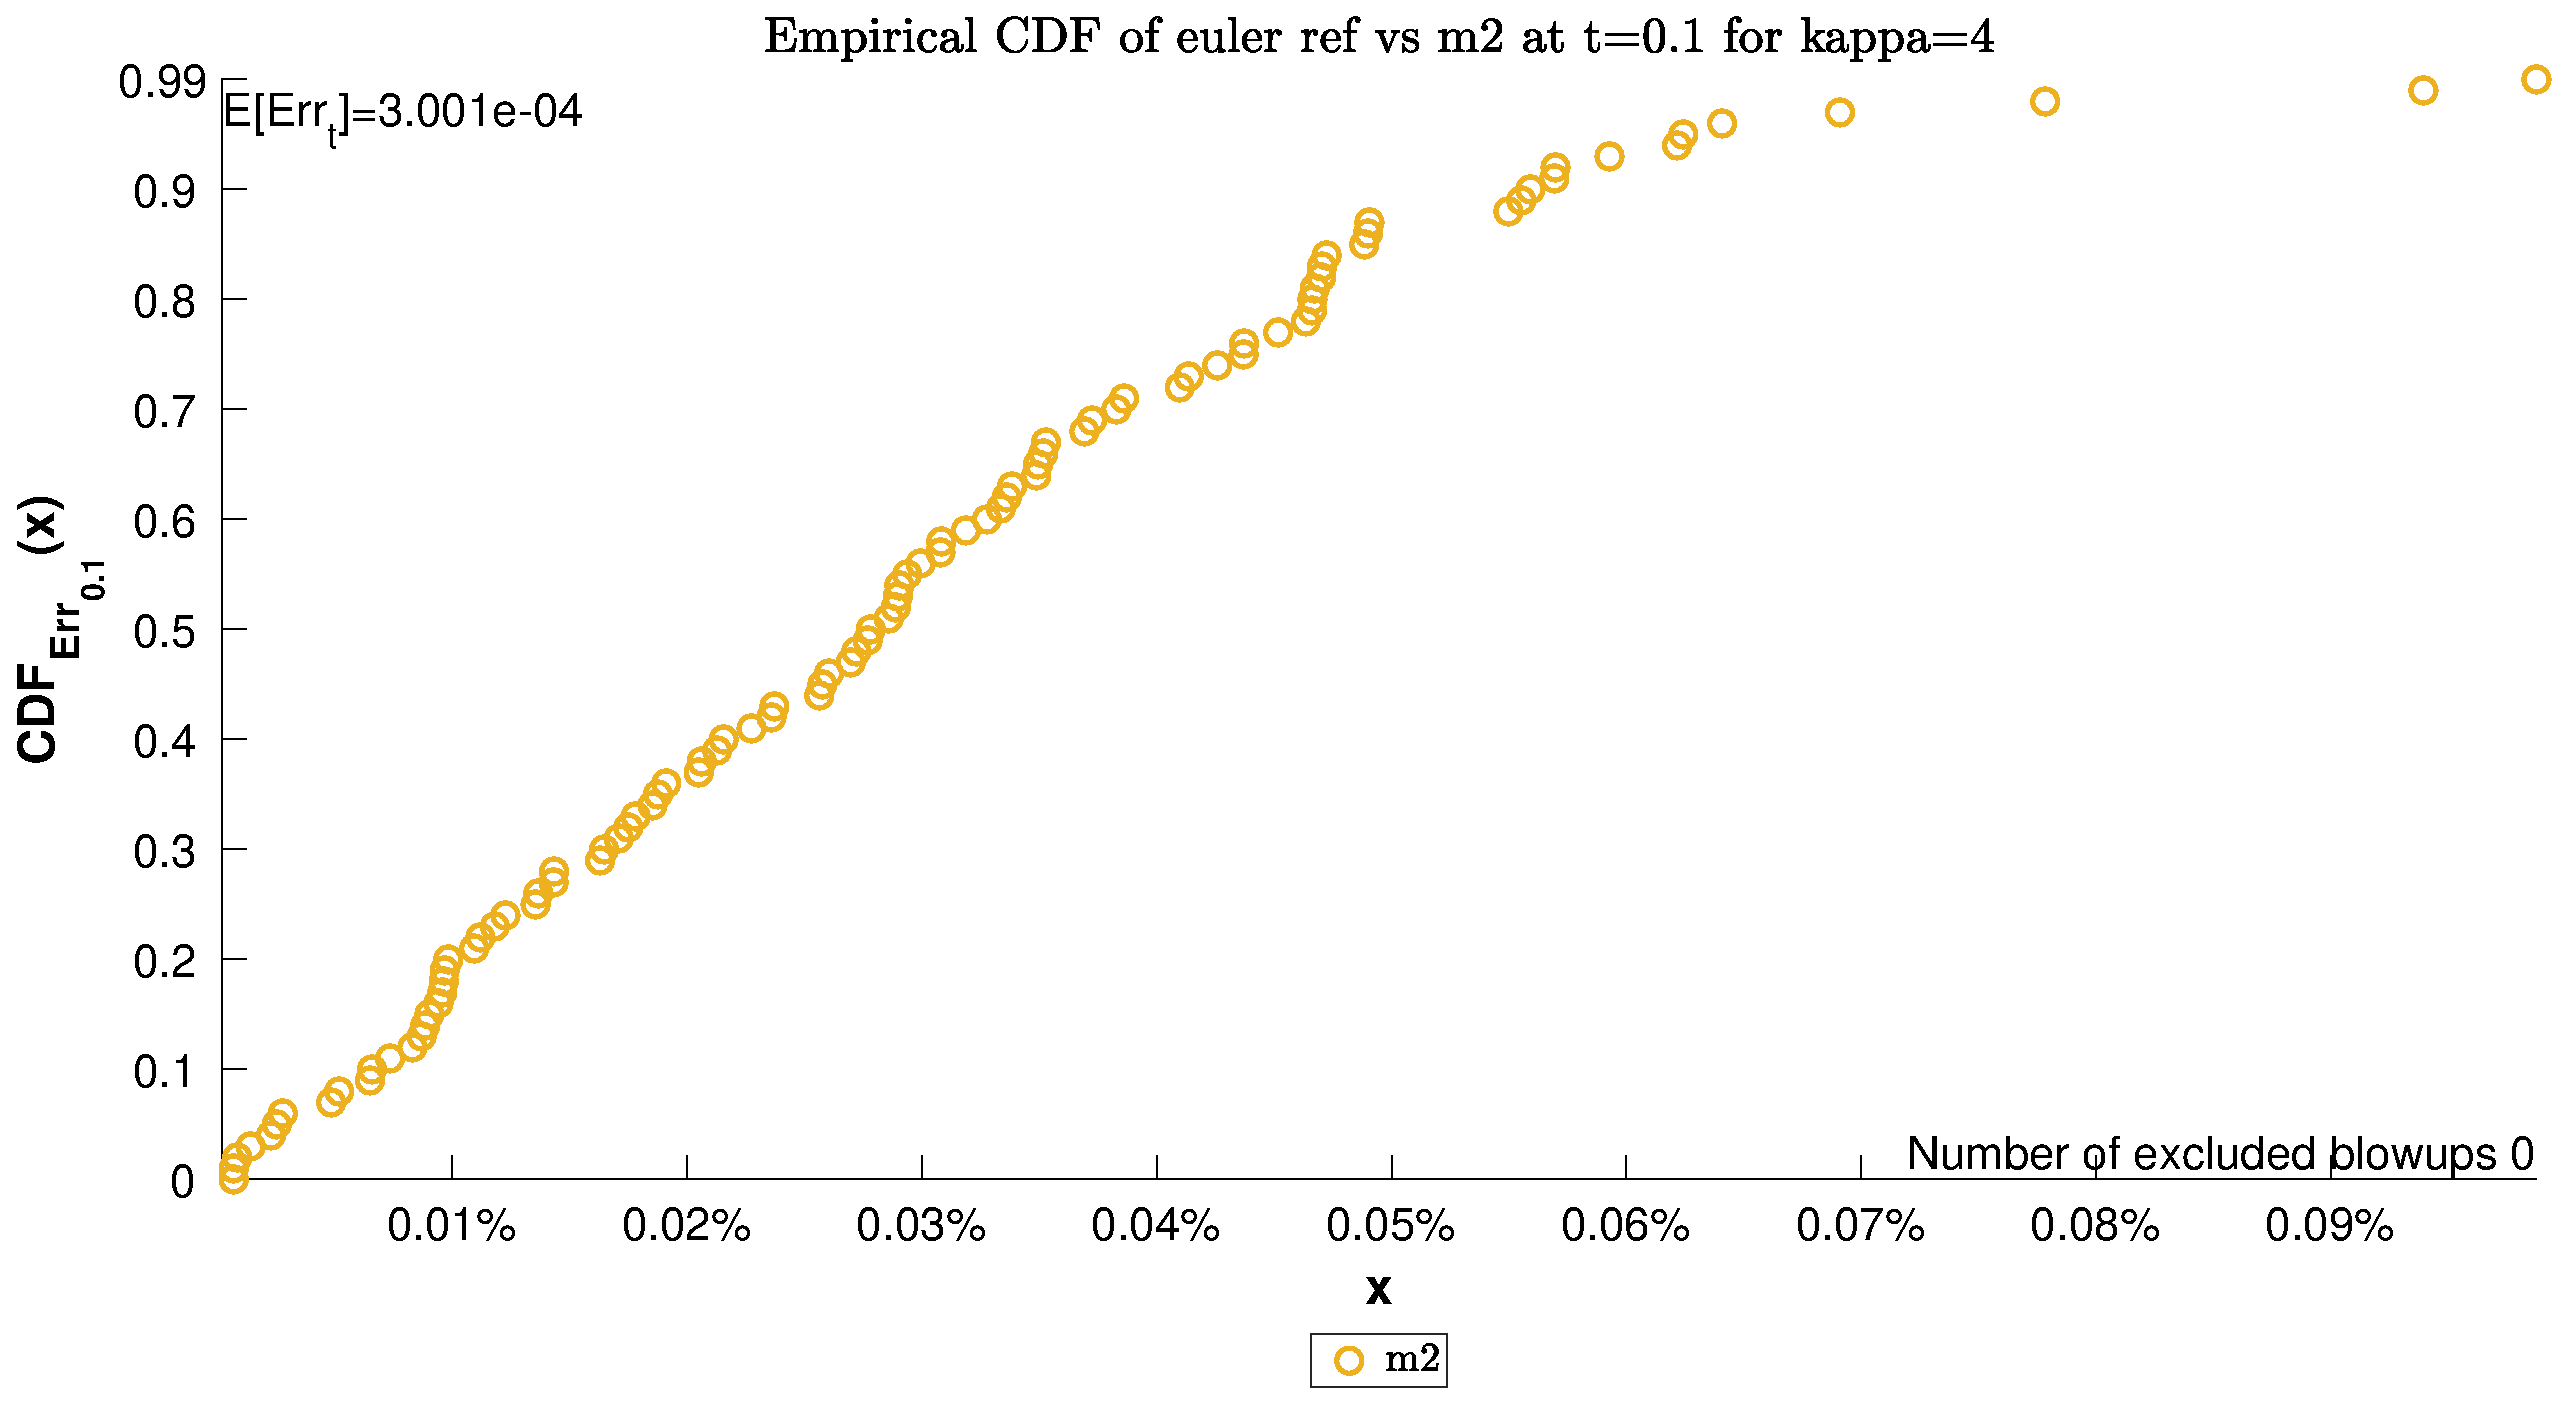
\includegraphics[width=.95\columnwidth]{CDF/CDFEulerRef_27}
\end{landscape}
\begin{landscape}
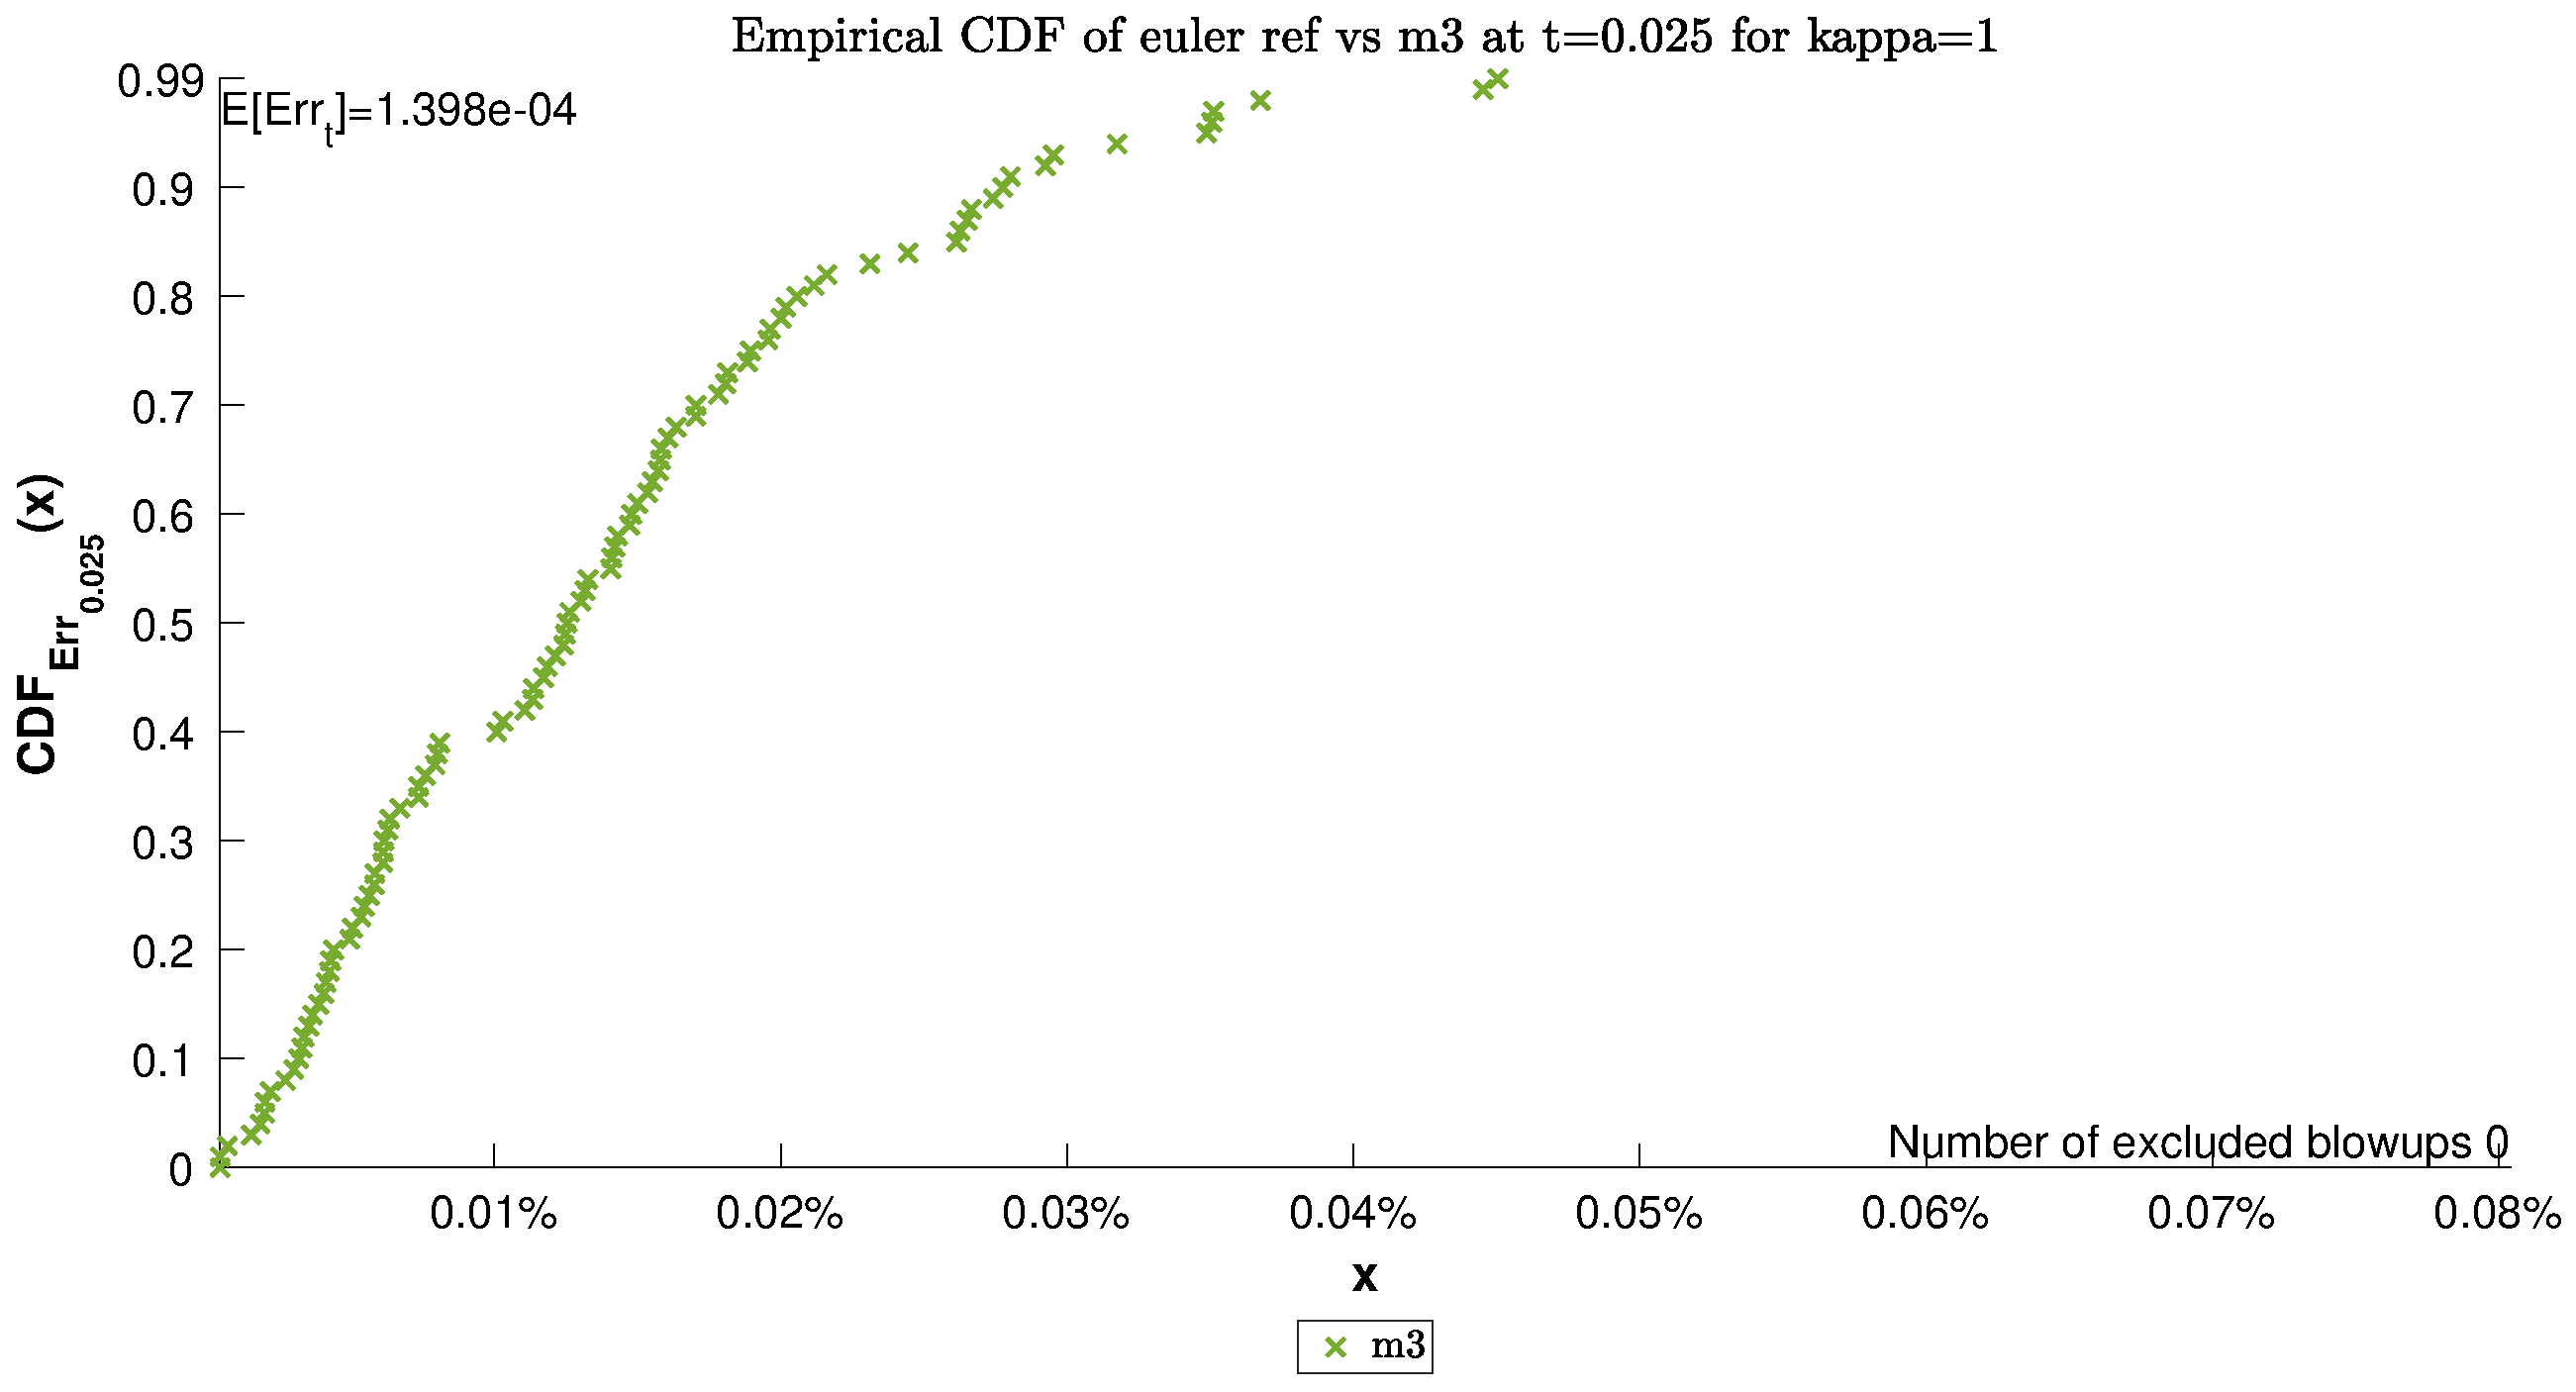
\includegraphics[width=.95\columnwidth]{CDF/CDFEulerRef_28}
\end{landscape}
\begin{landscape}
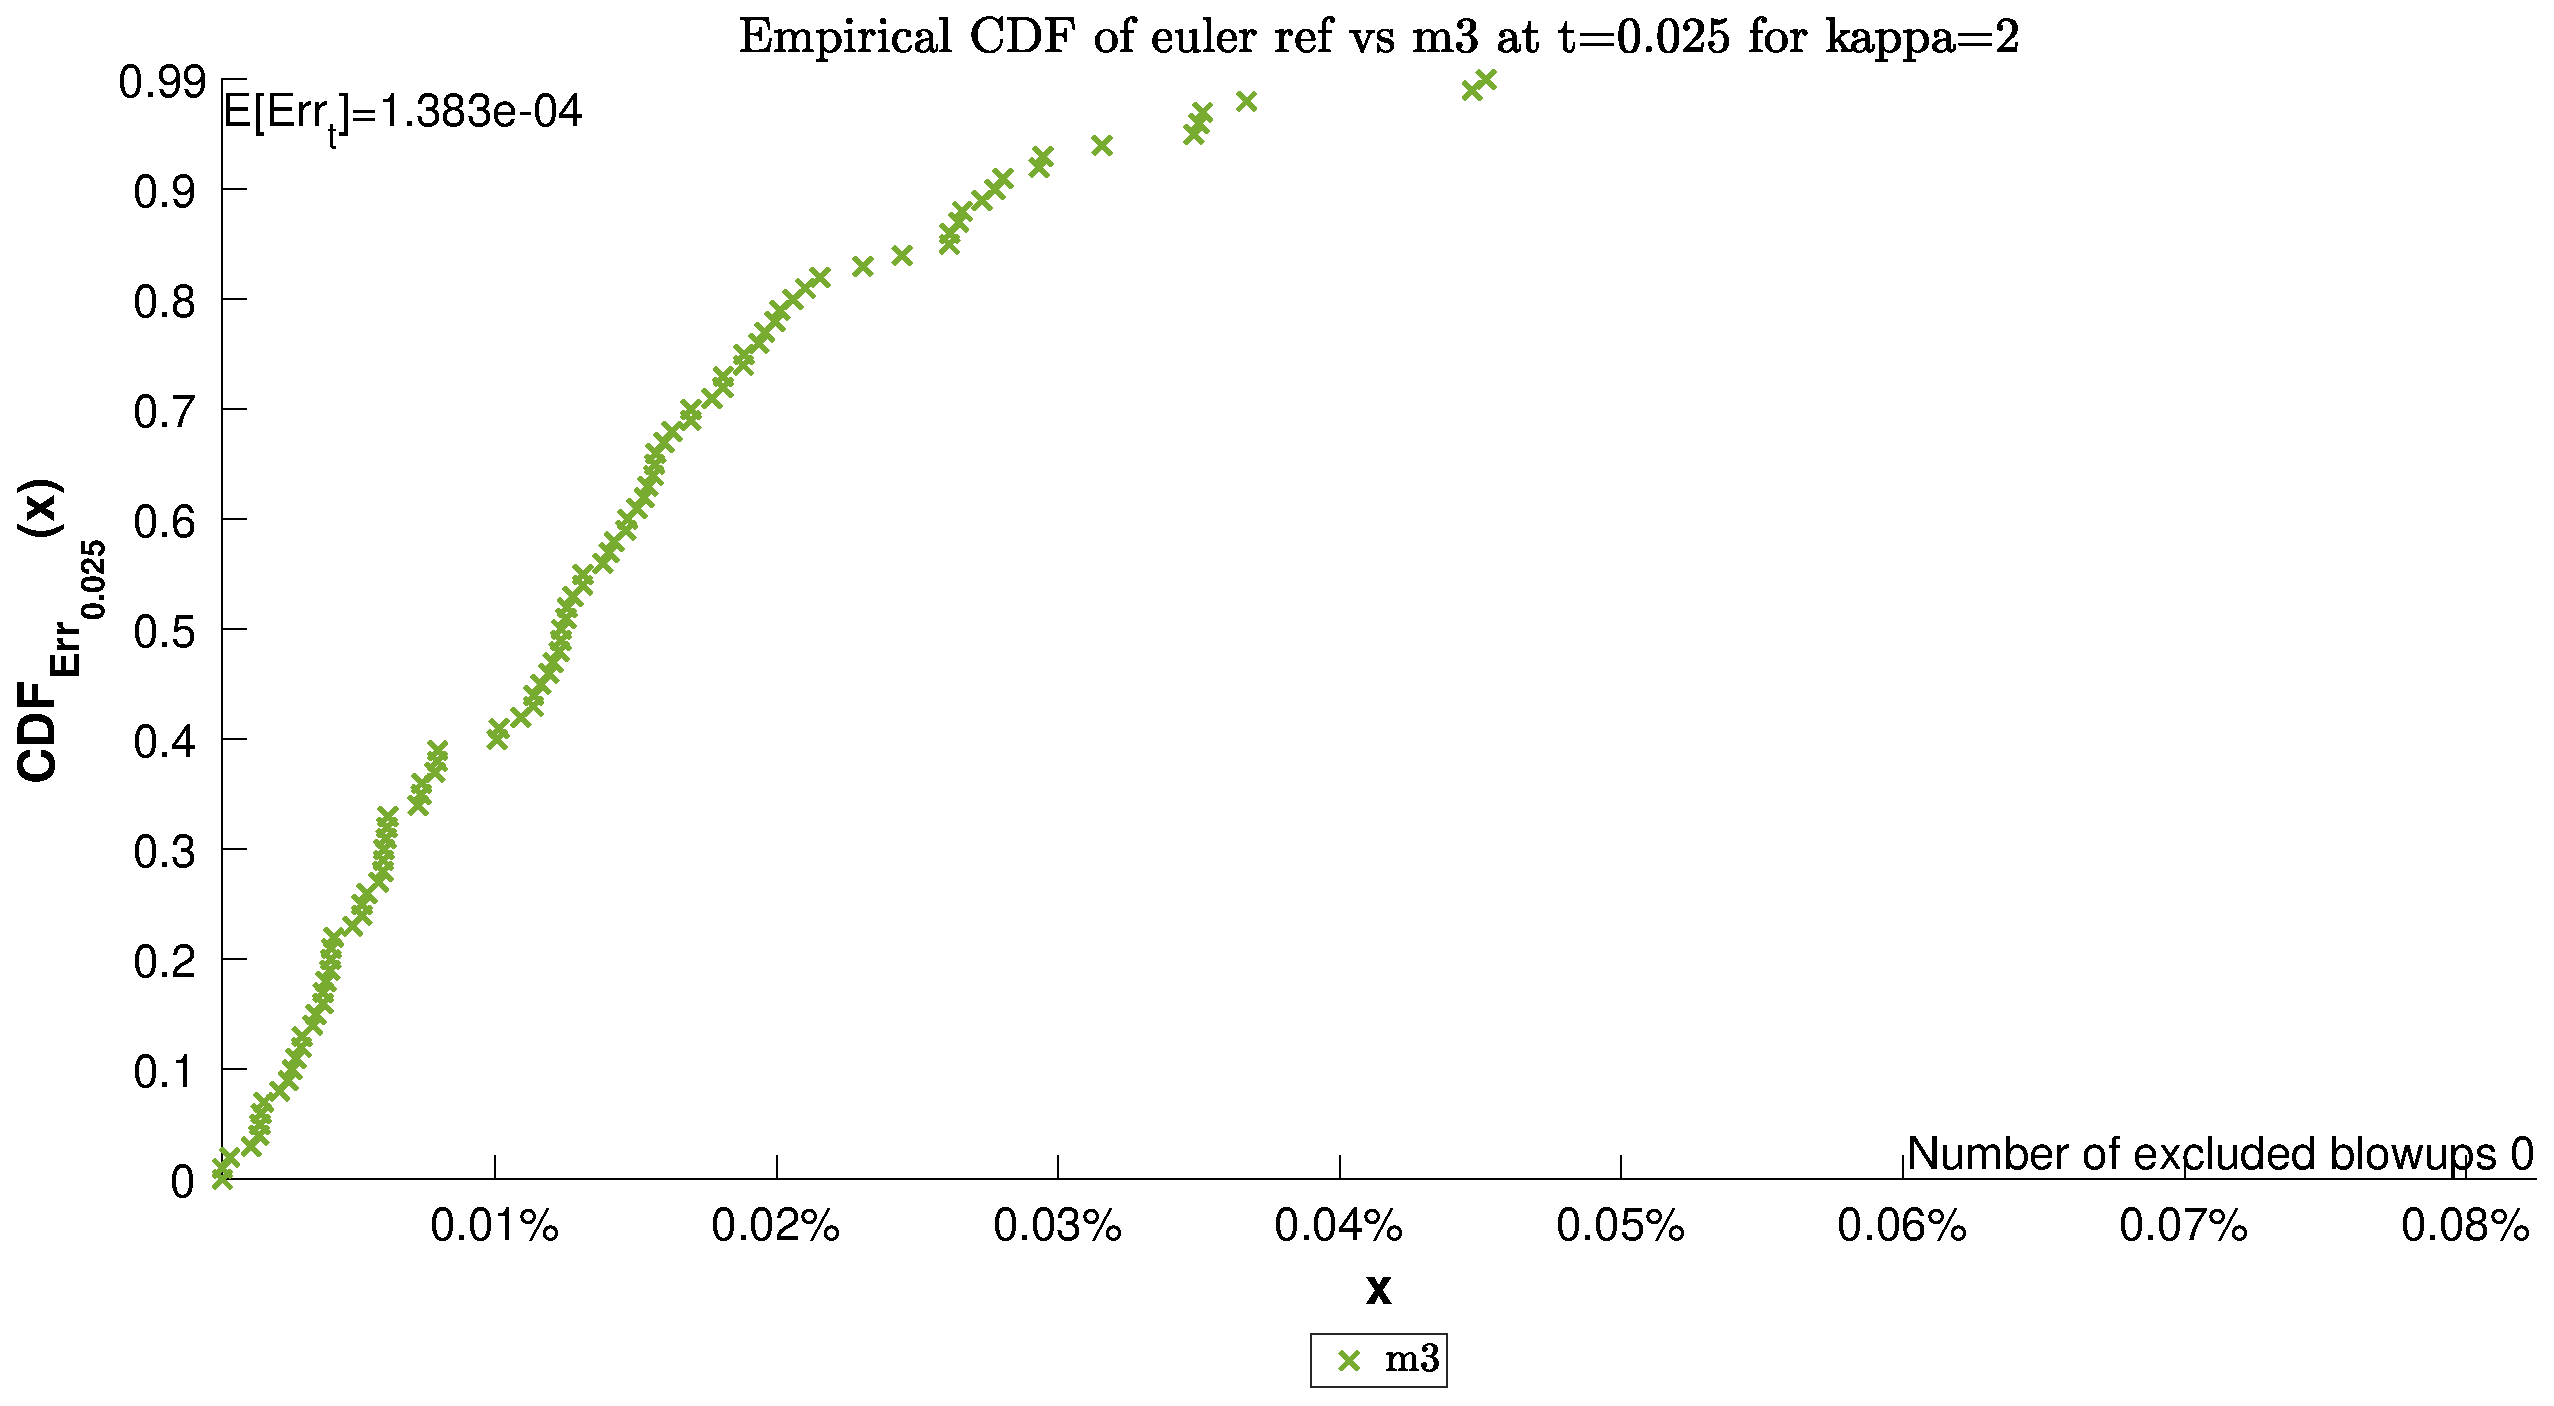
\includegraphics[width=.95\columnwidth]{CDF/CDFEulerRef_29}
\end{landscape}
\begin{landscape}
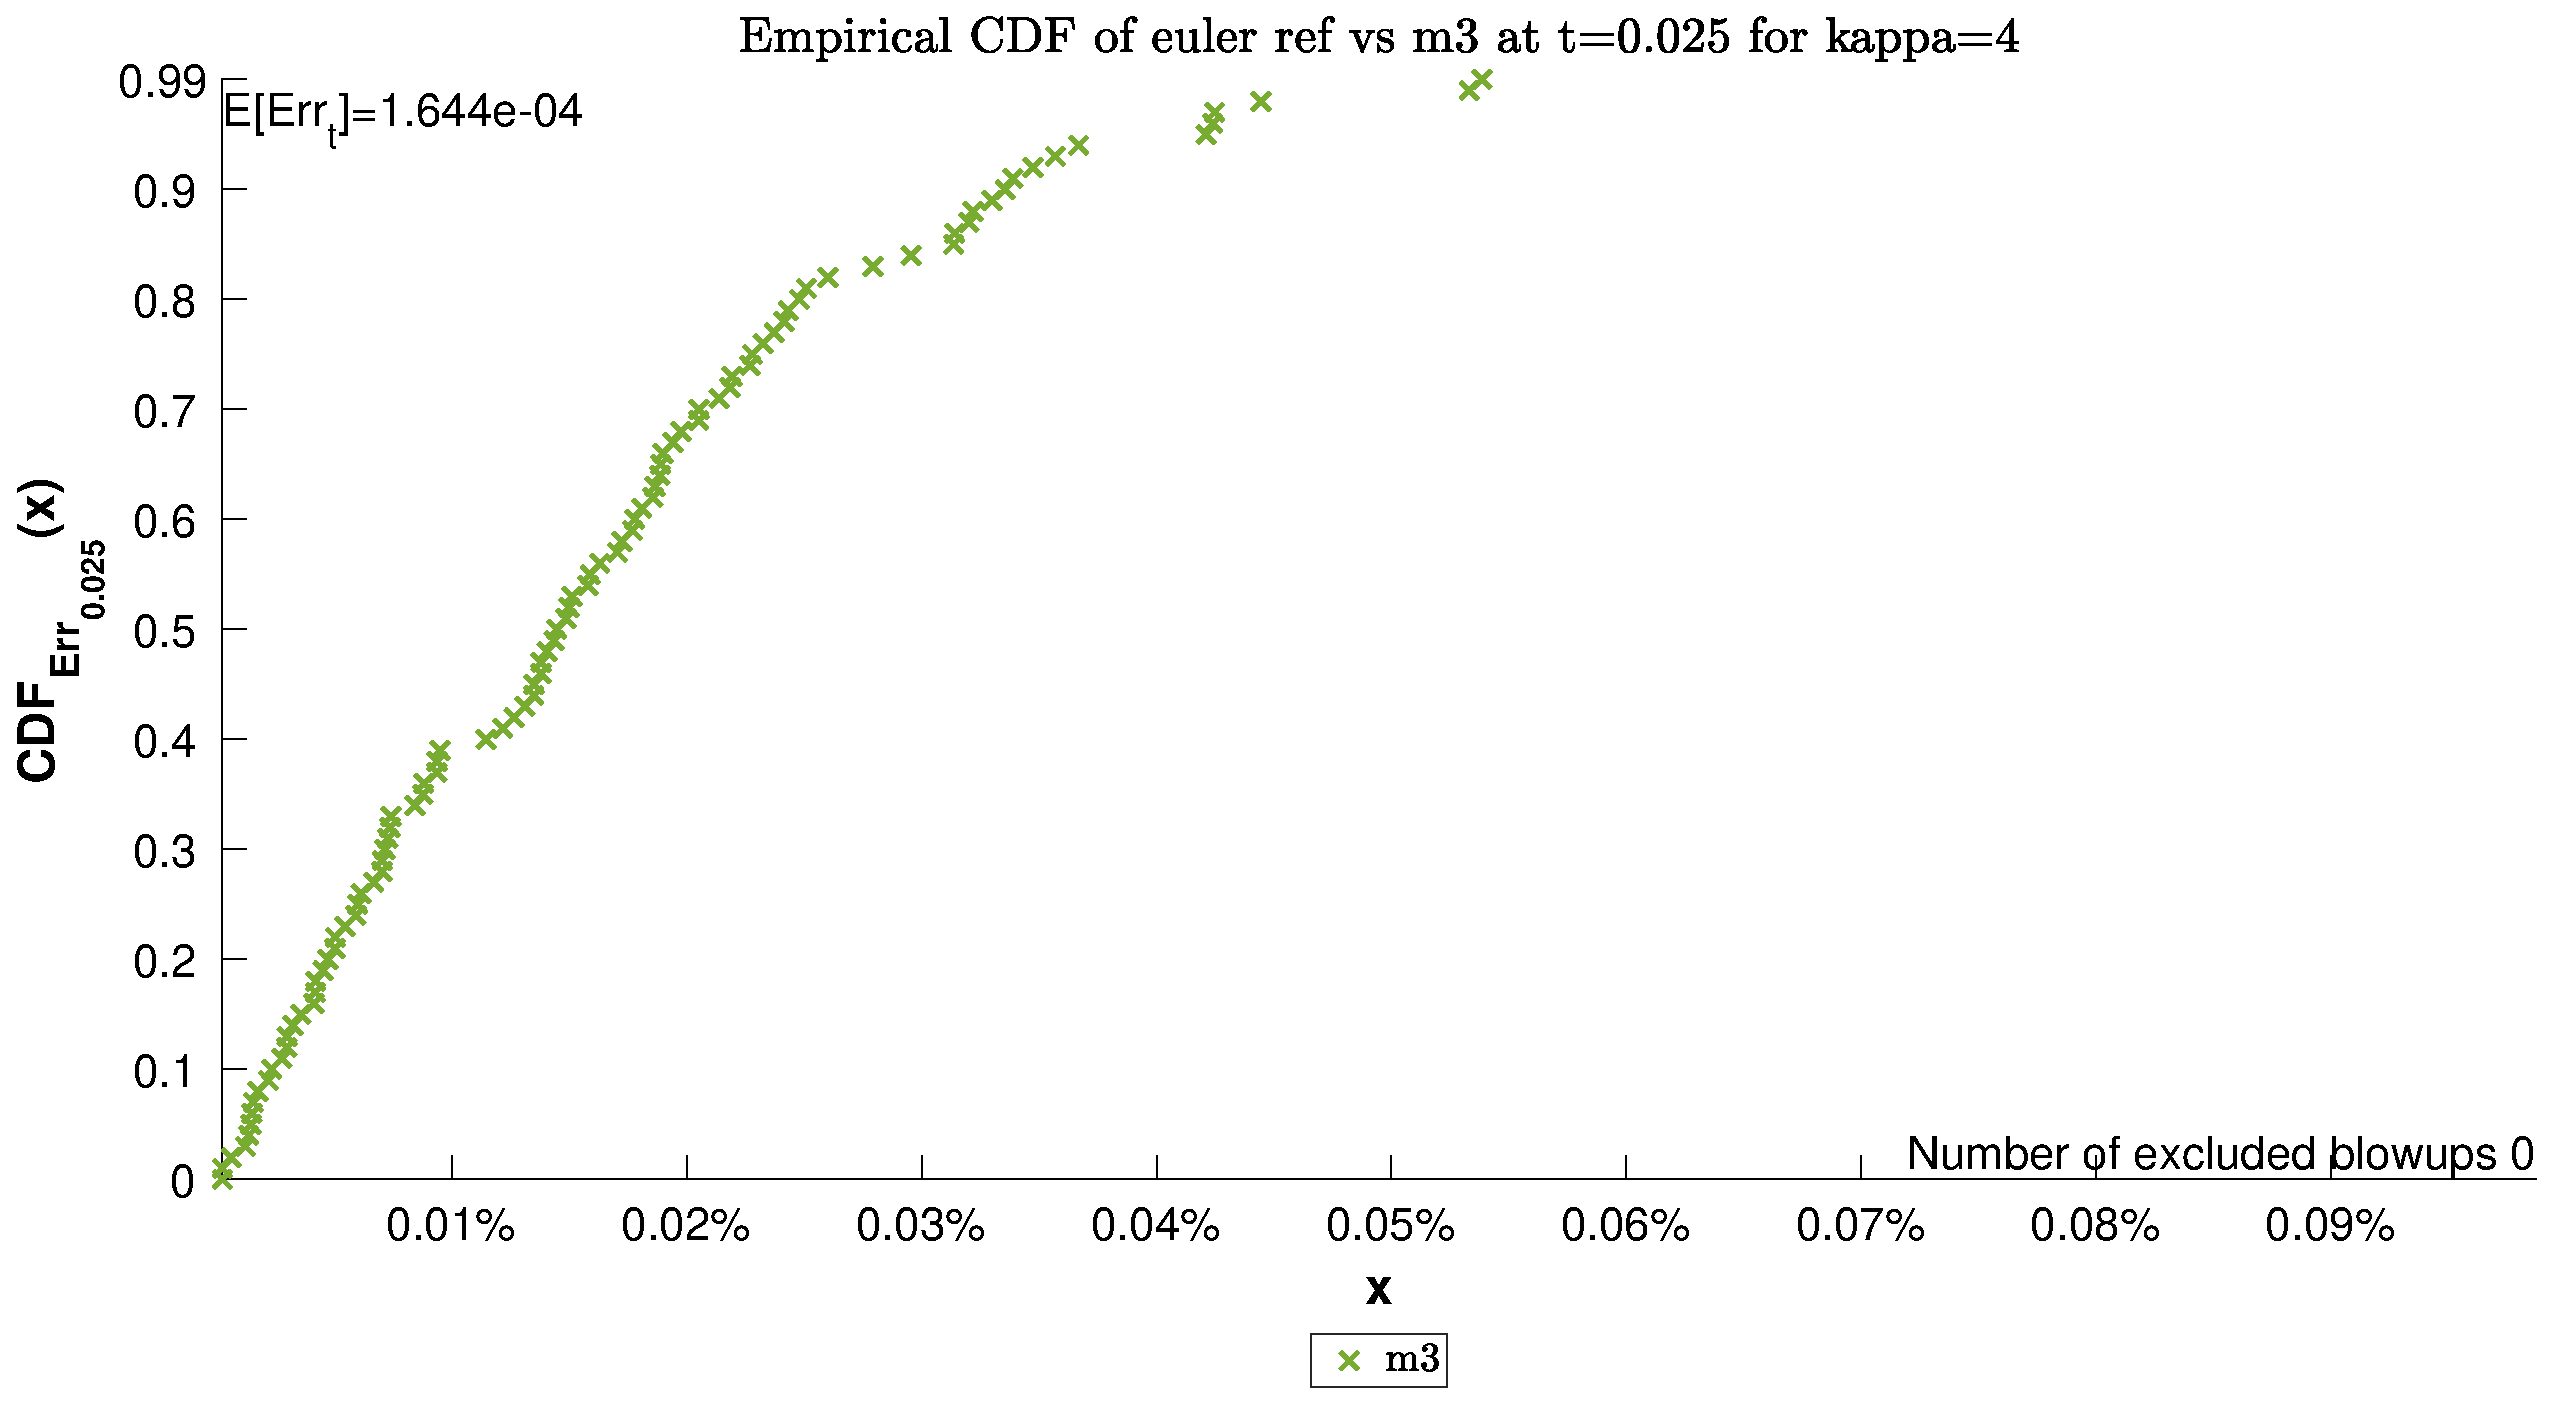
\includegraphics[width=.95\columnwidth]{CDF/CDFEulerRef_30}
\end{landscape}
\begin{landscape}
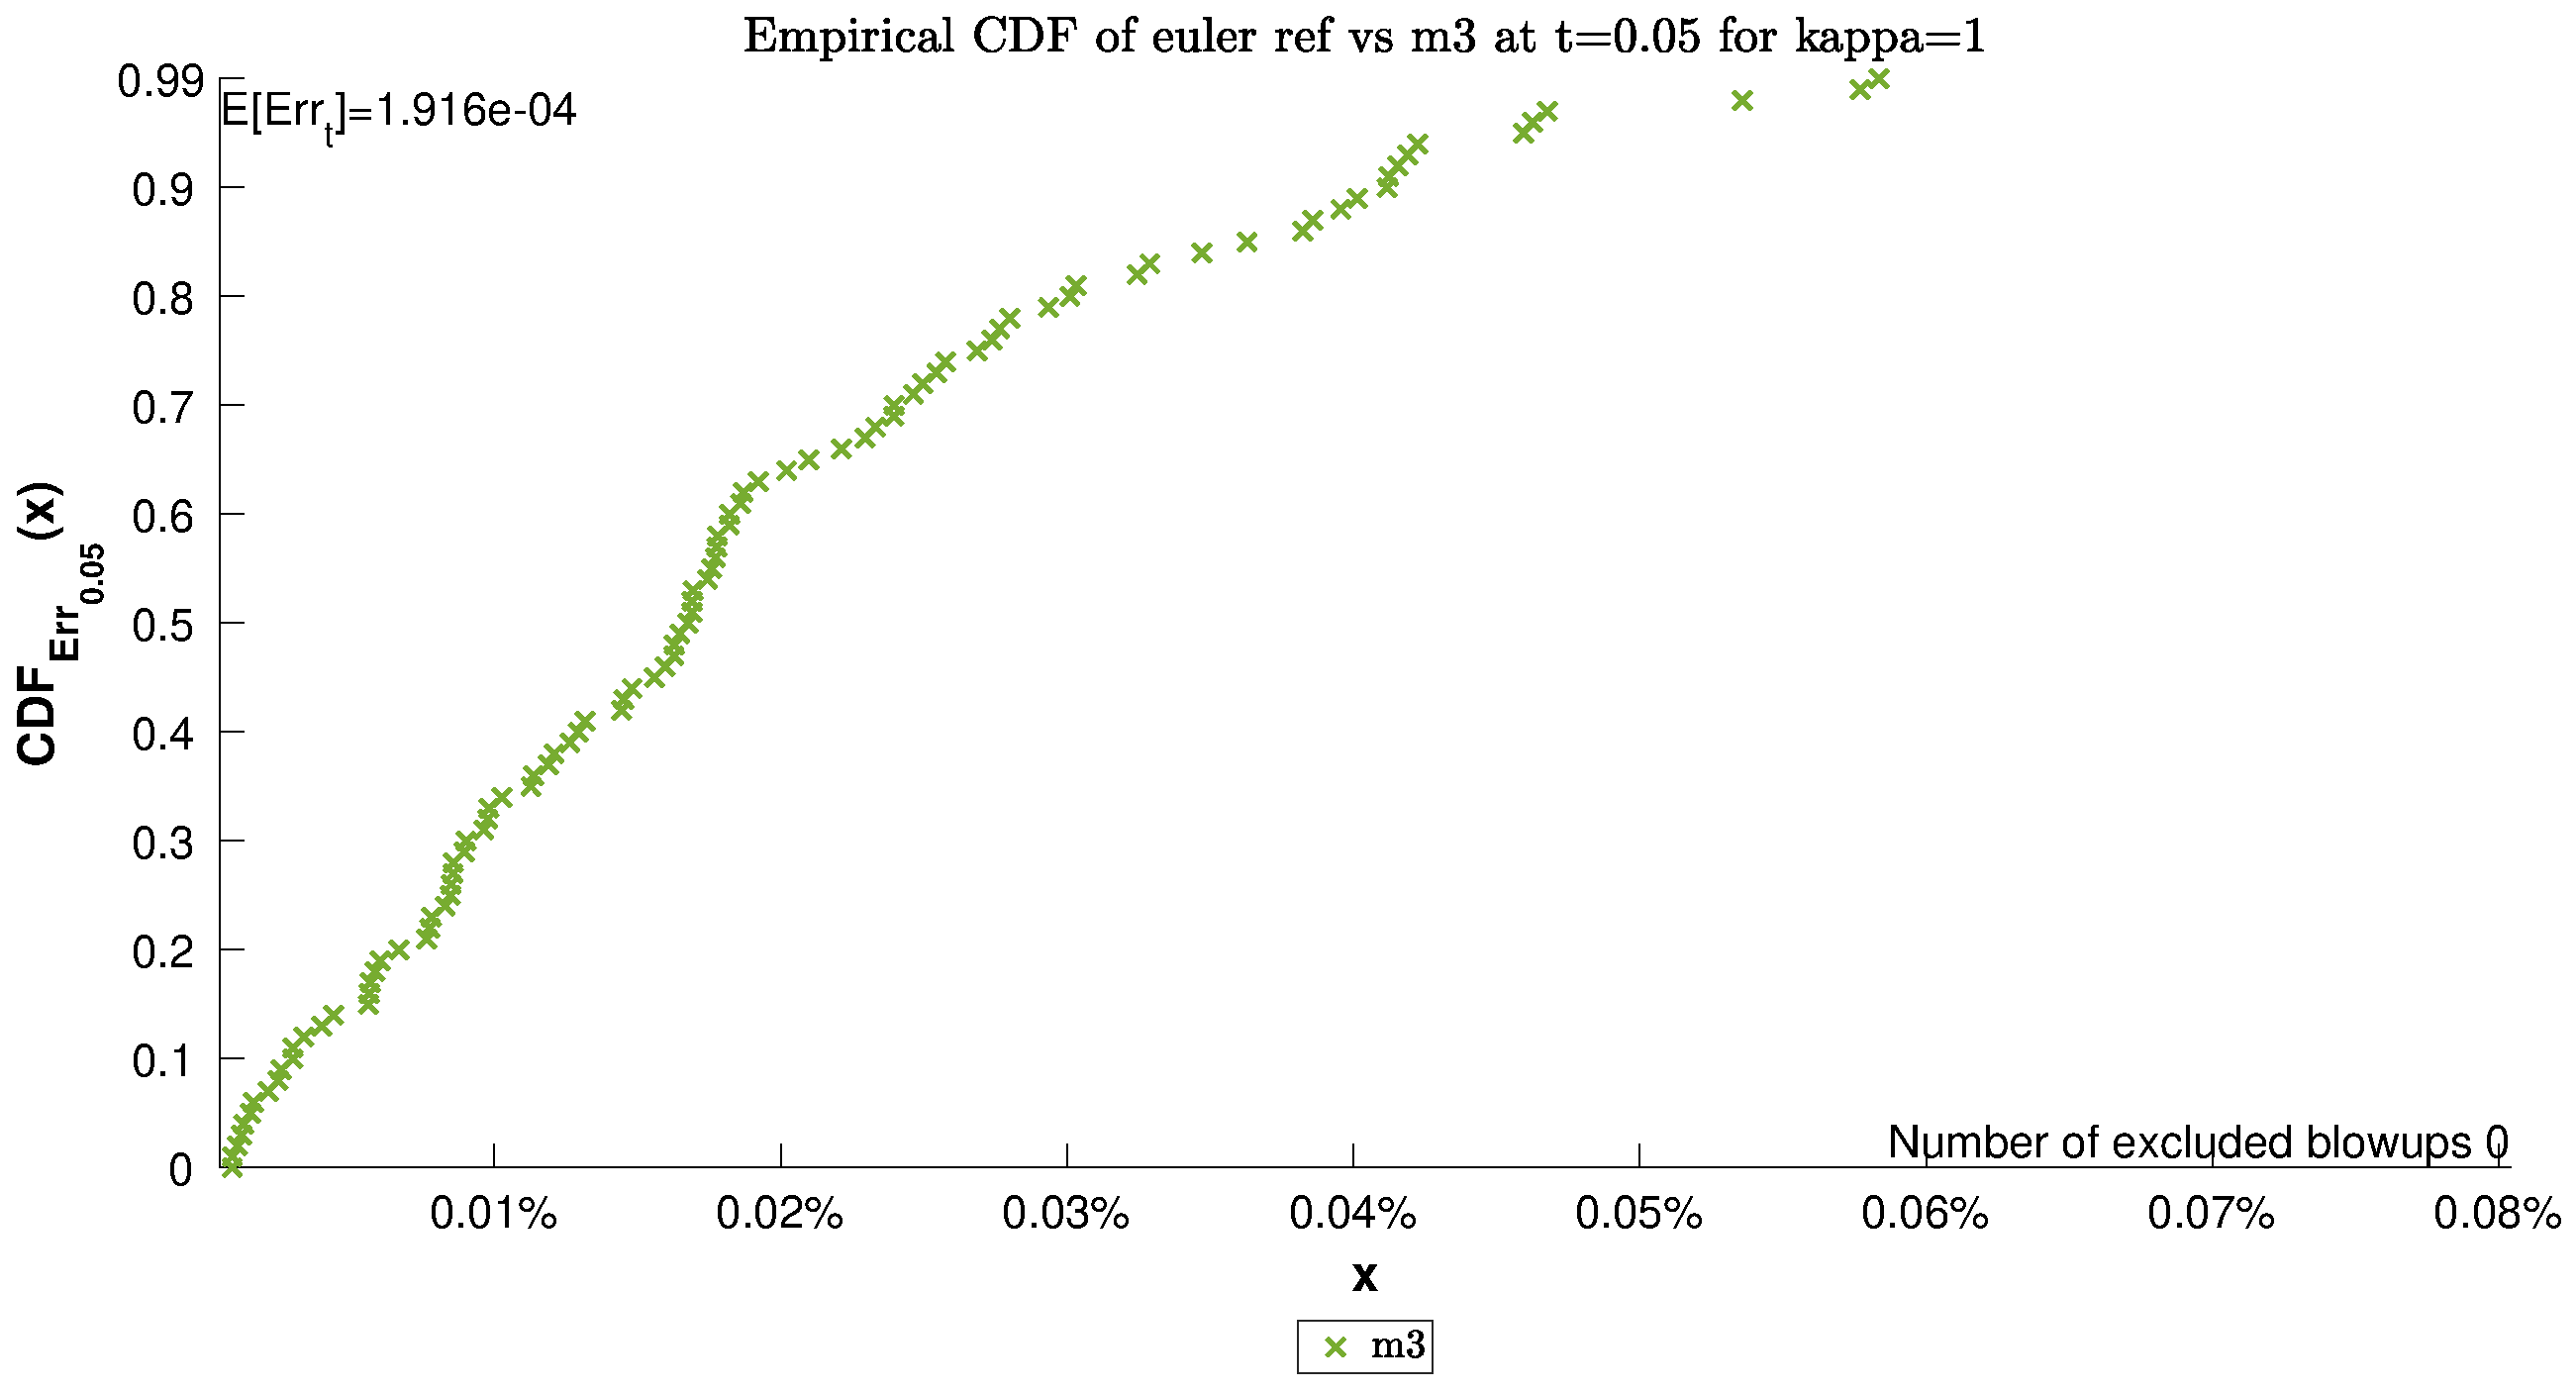
\includegraphics[width=.95\columnwidth]{CDF/CDFEulerRef_31}
\end{landscape}
\begin{landscape}
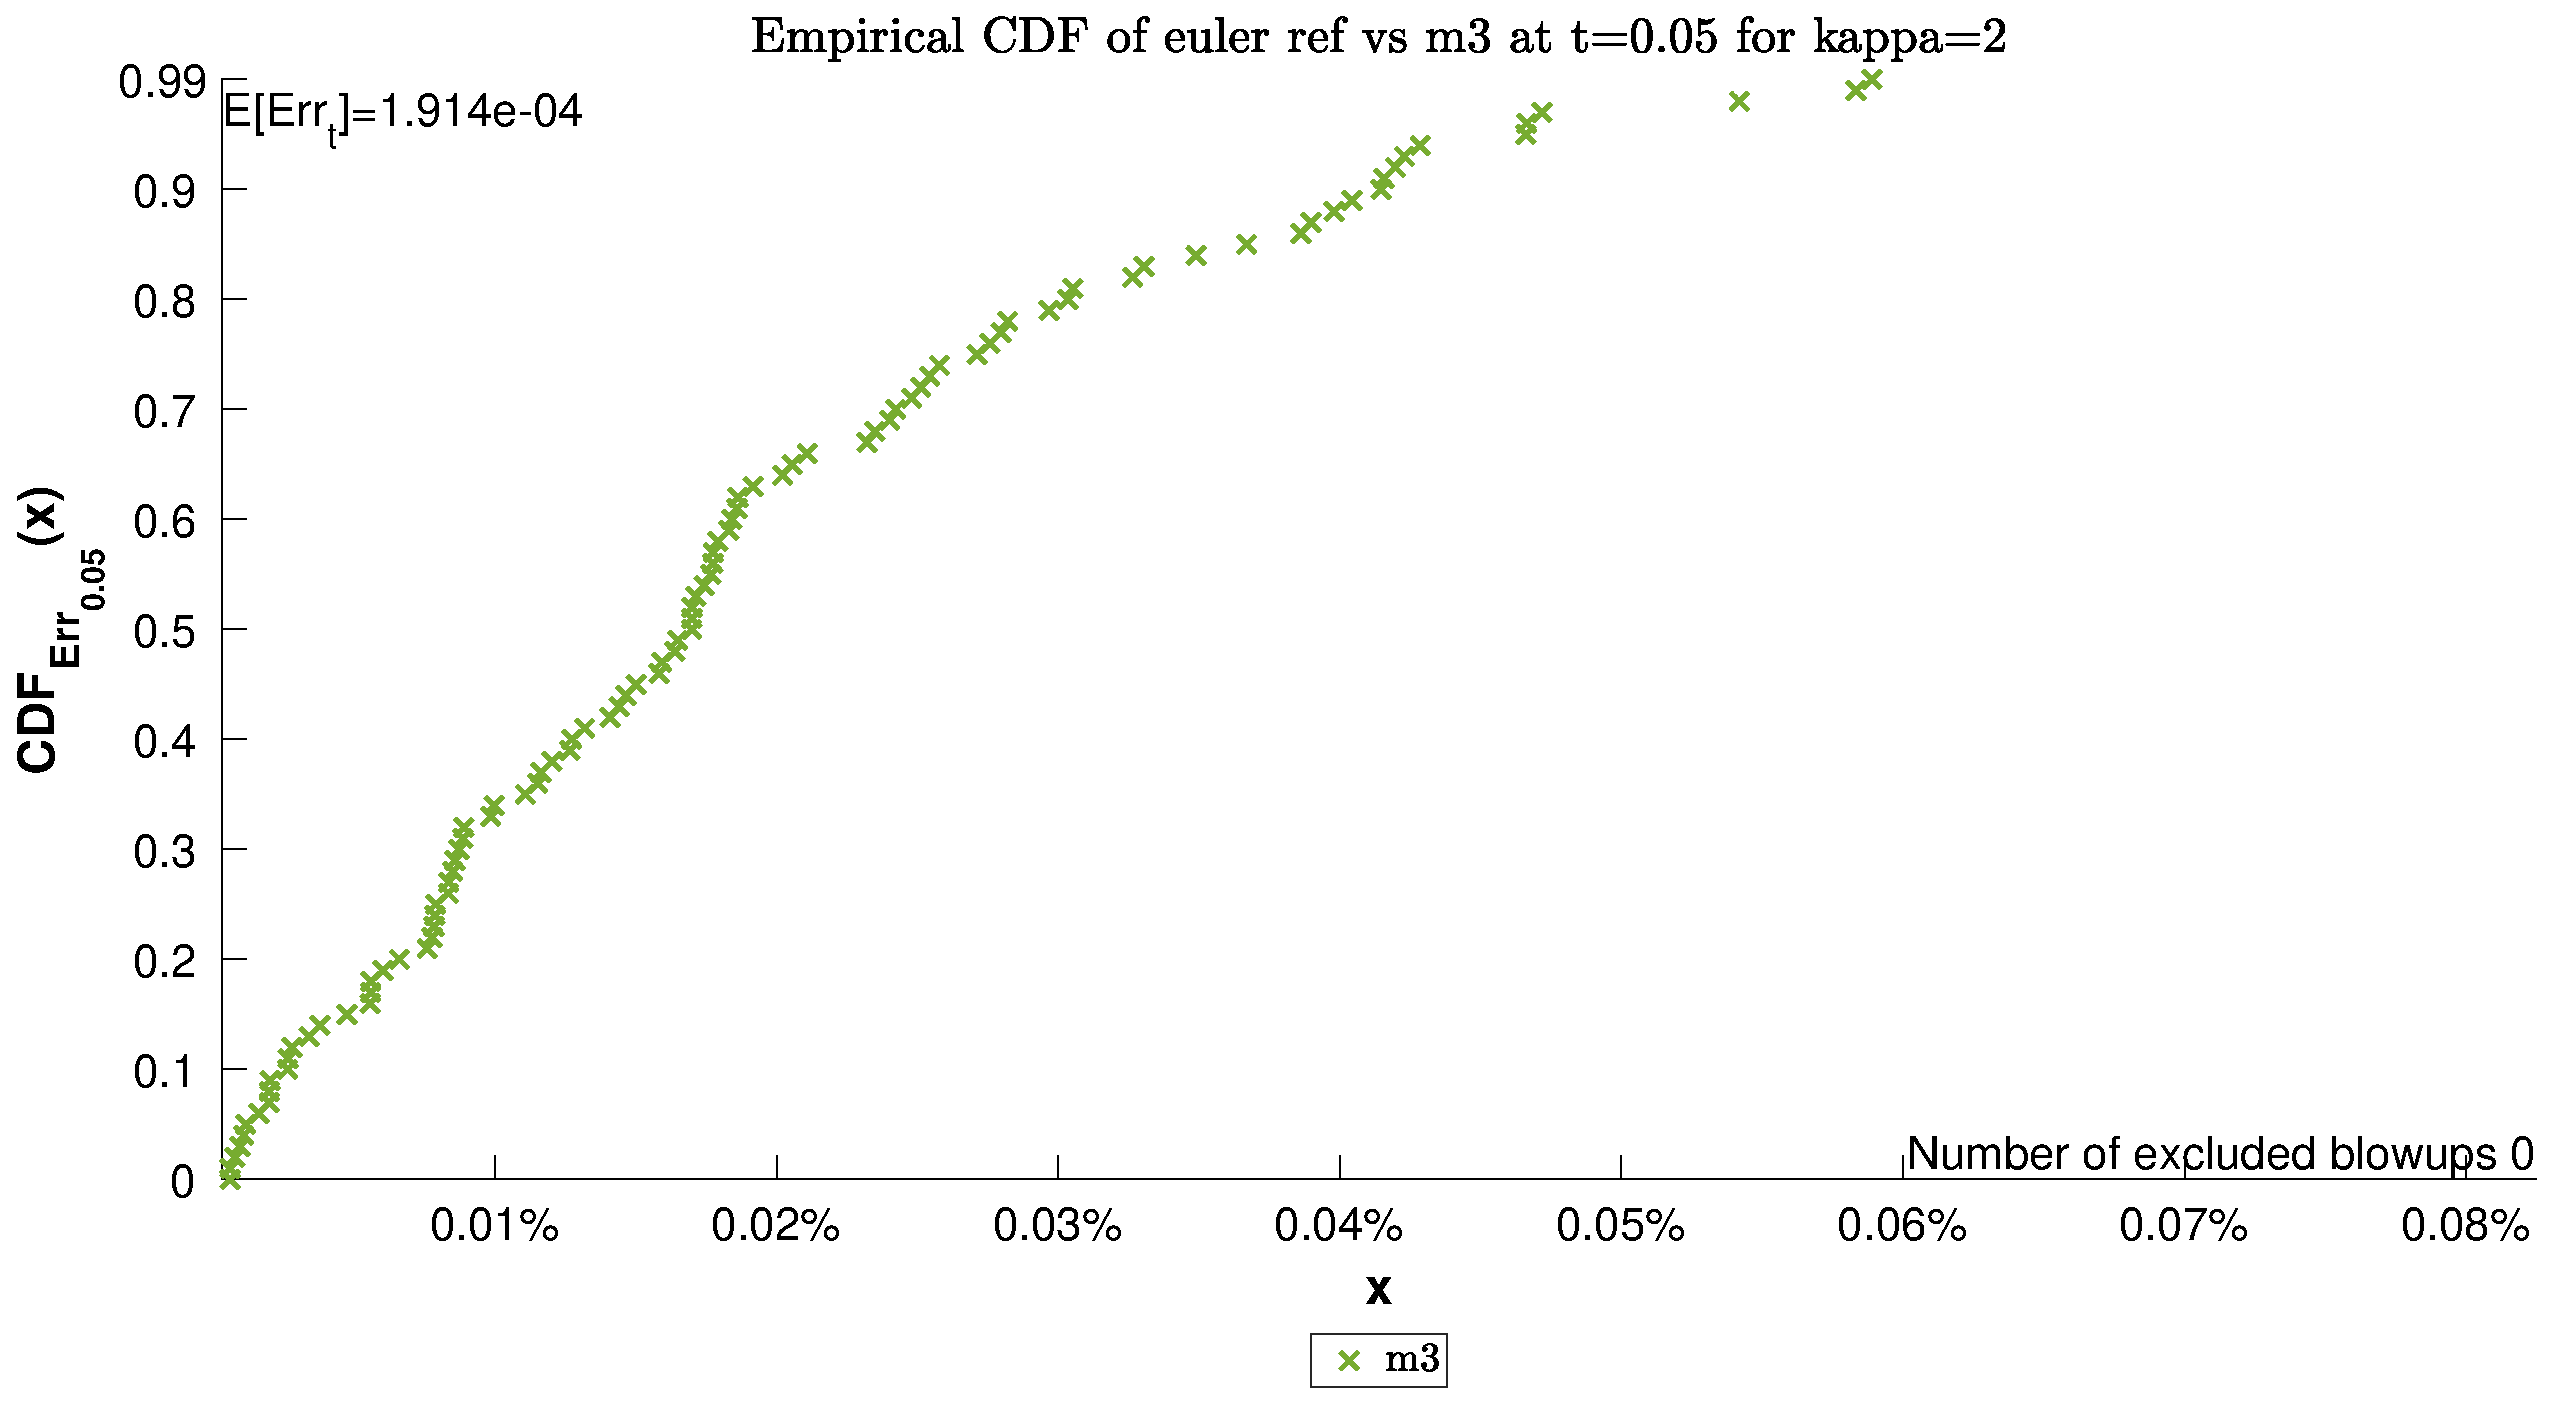
\includegraphics[width=.95\columnwidth]{CDF/CDFEulerRef_32}
\end{landscape}
\begin{landscape}
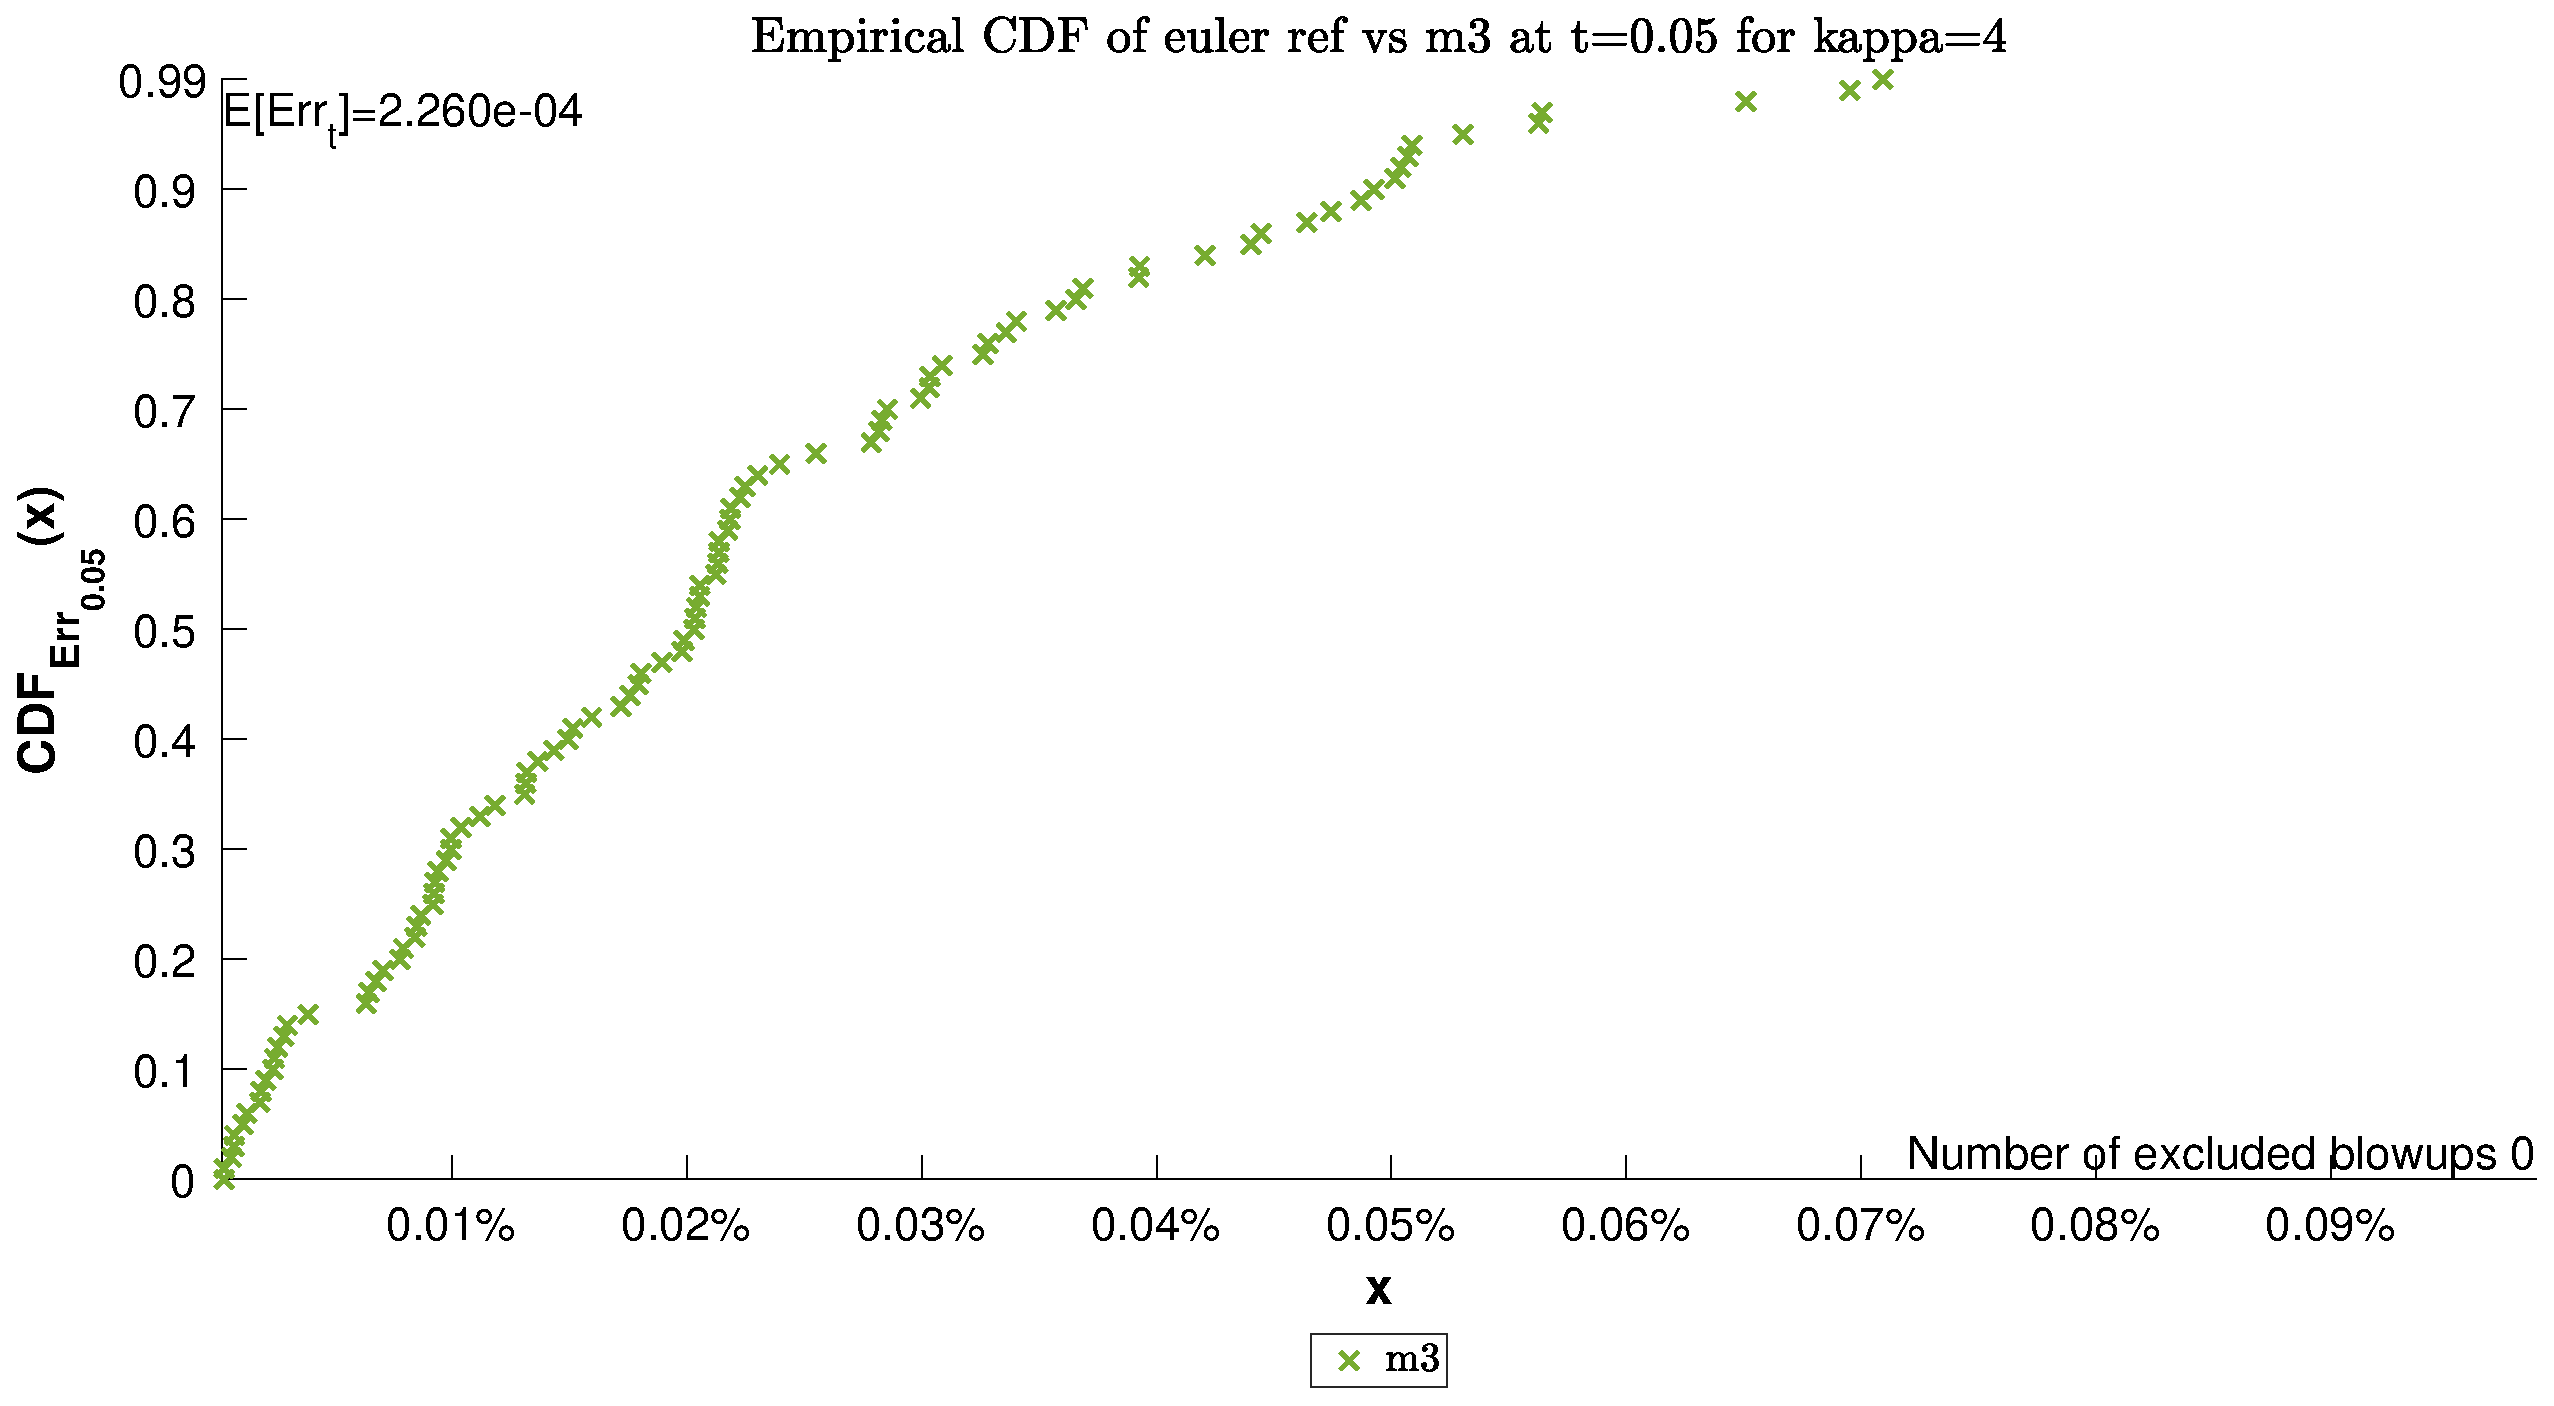
\includegraphics[width=.95\columnwidth]{CDF/CDFEulerRef_33}
\end{landscape}
\begin{landscape}
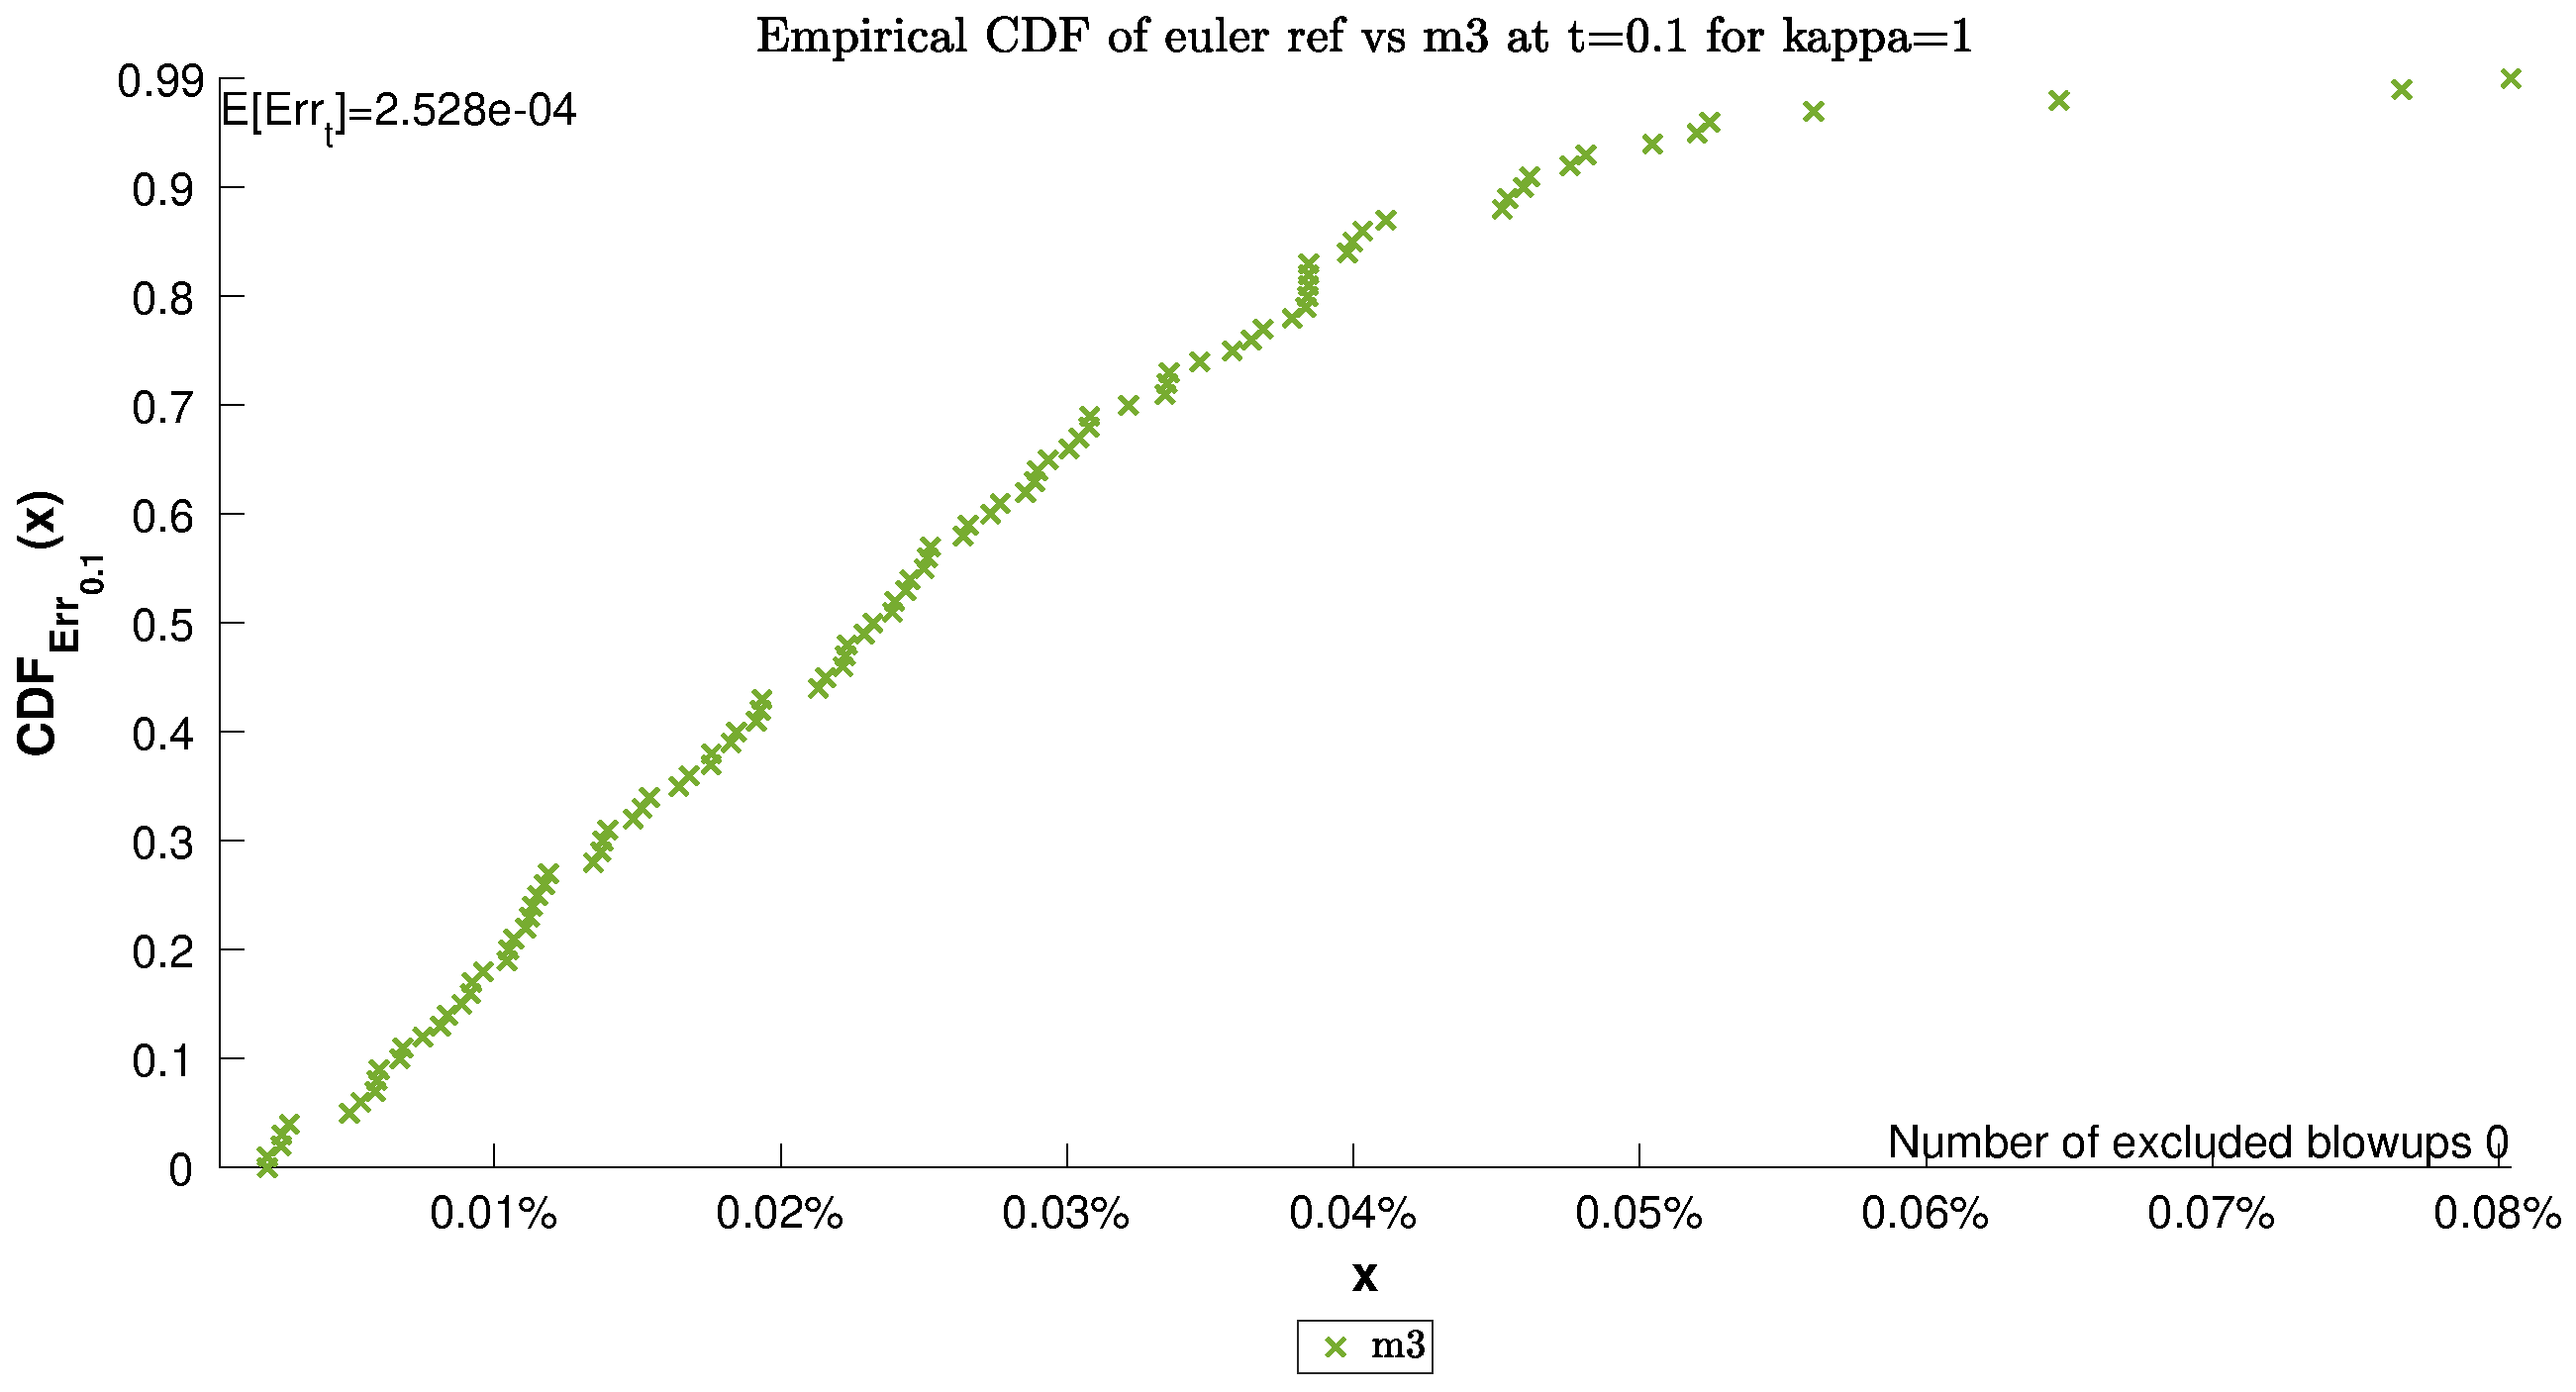
\includegraphics[width=.95\columnwidth]{CDF/CDFEulerRef_34}
\end{landscape}
\begin{landscape}
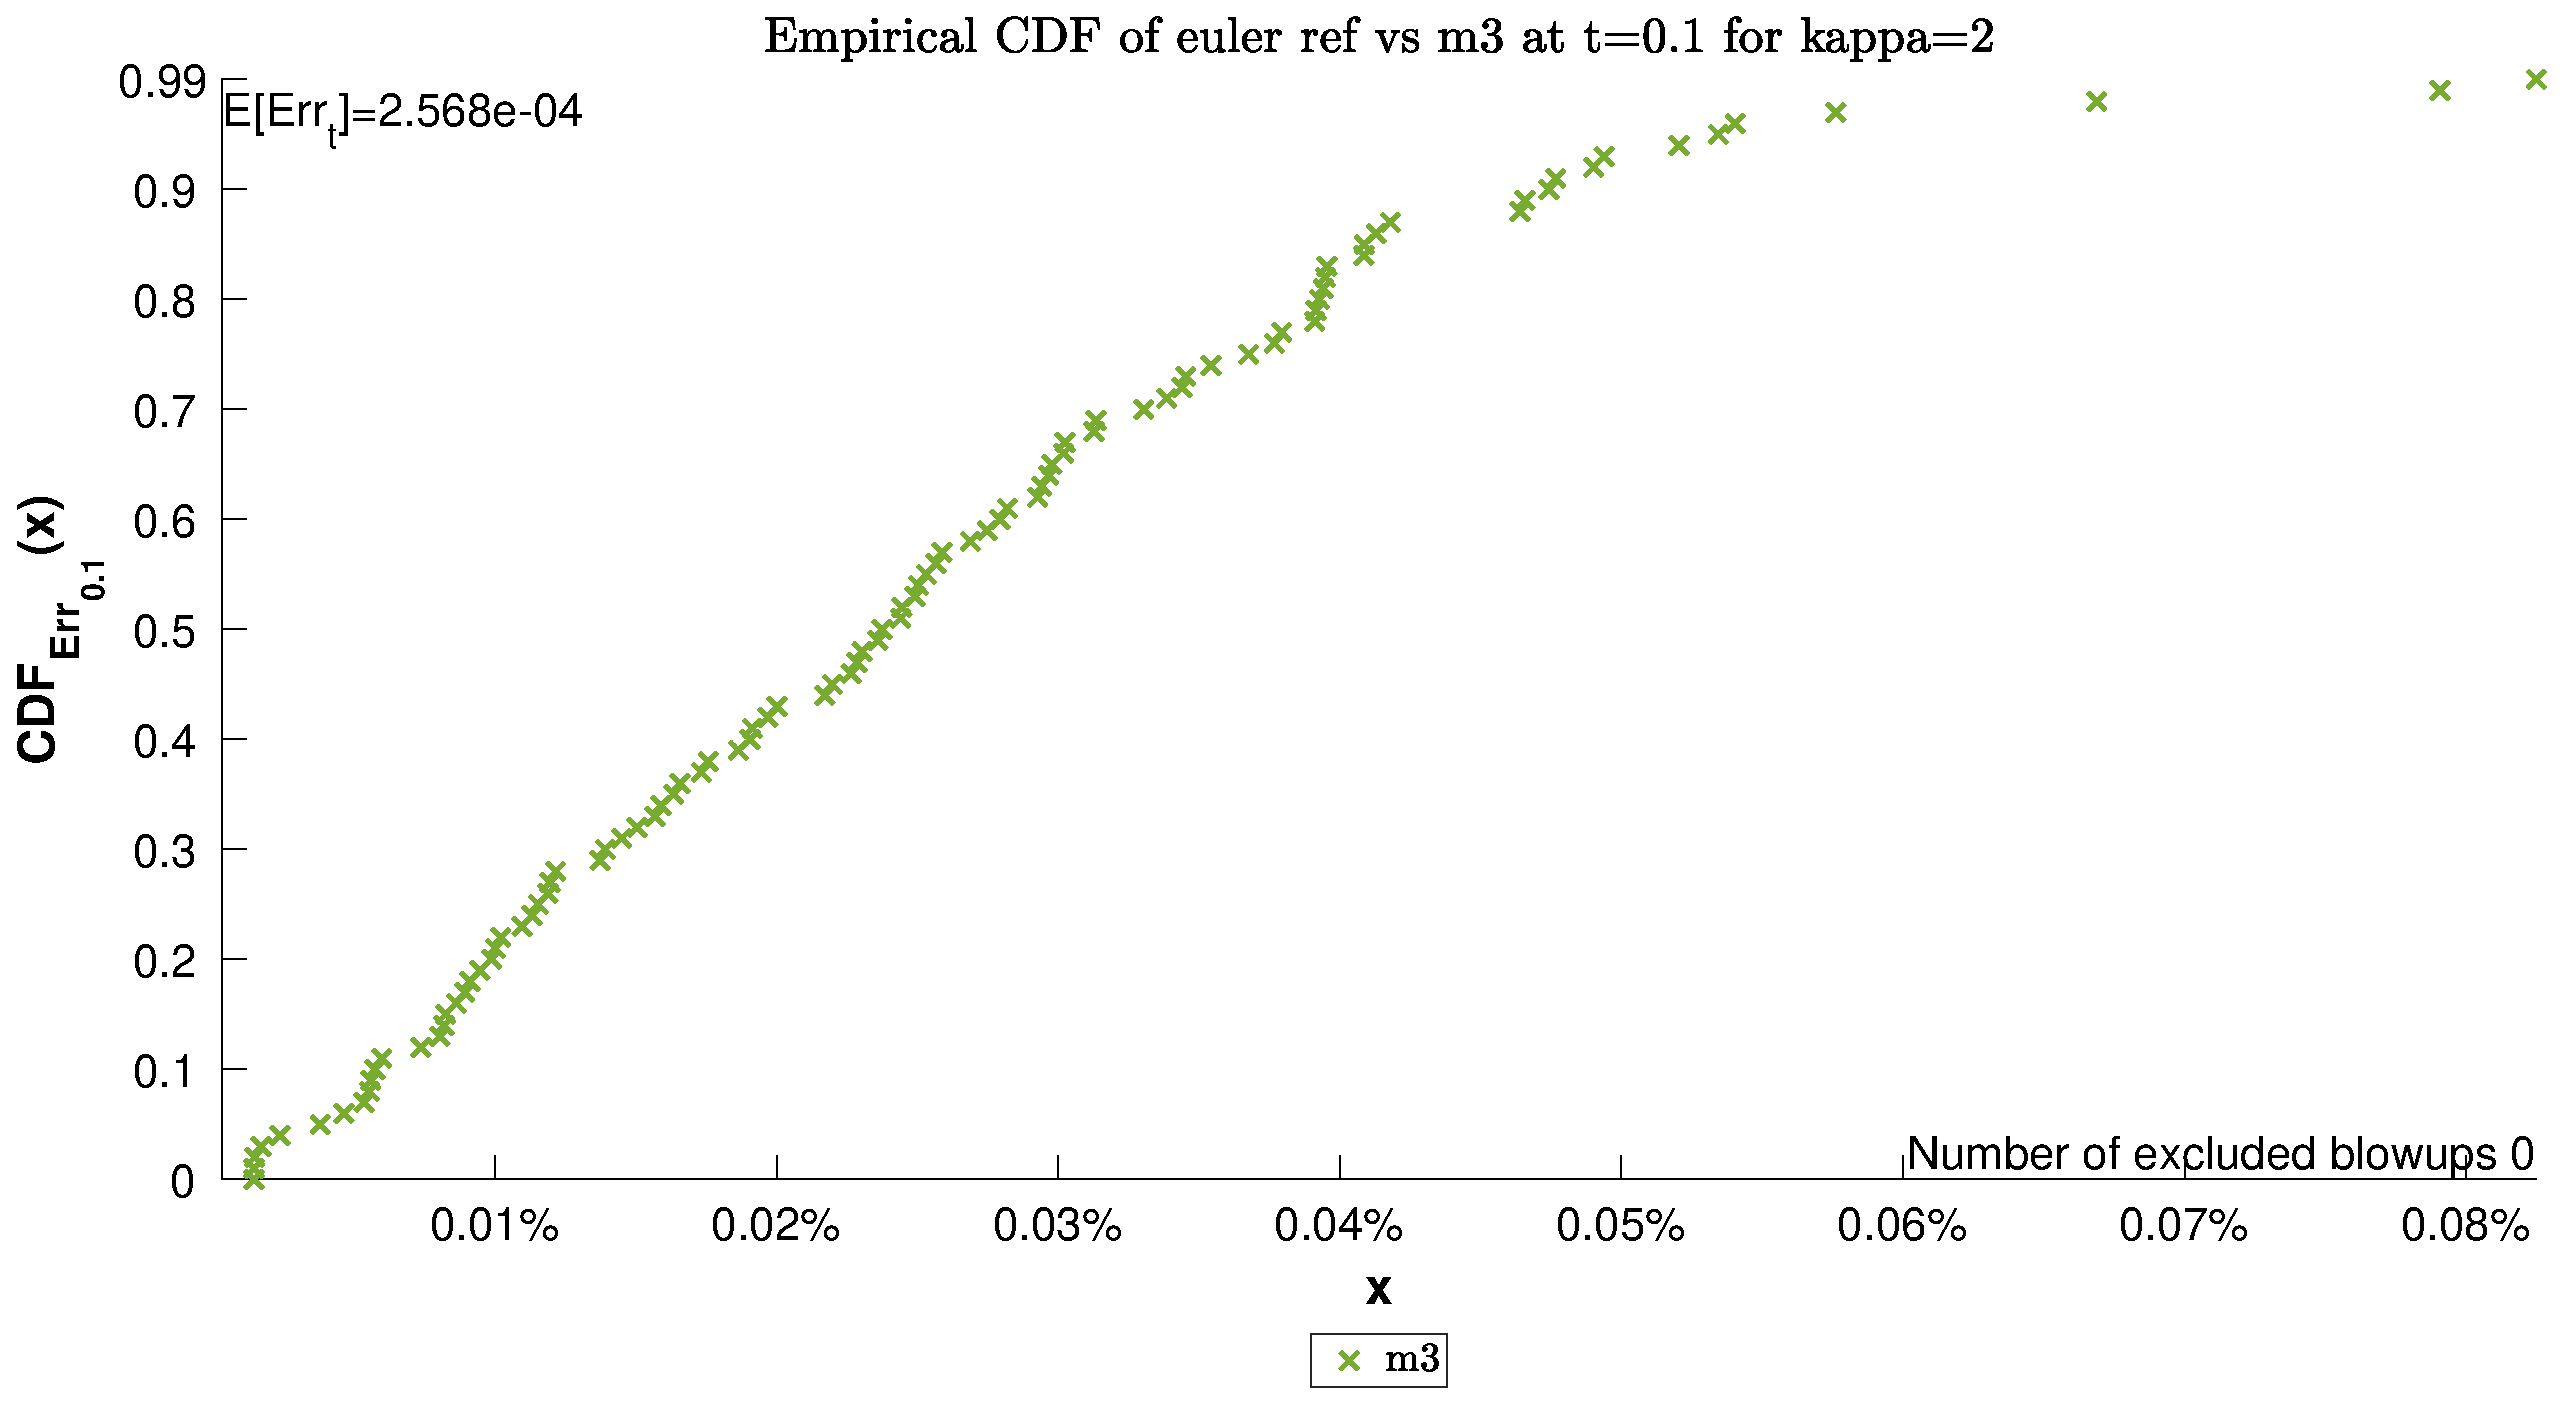
\includegraphics[width=.95\columnwidth]{CDF/CDFEulerRef_35}
\end{landscape}
\begin{landscape}
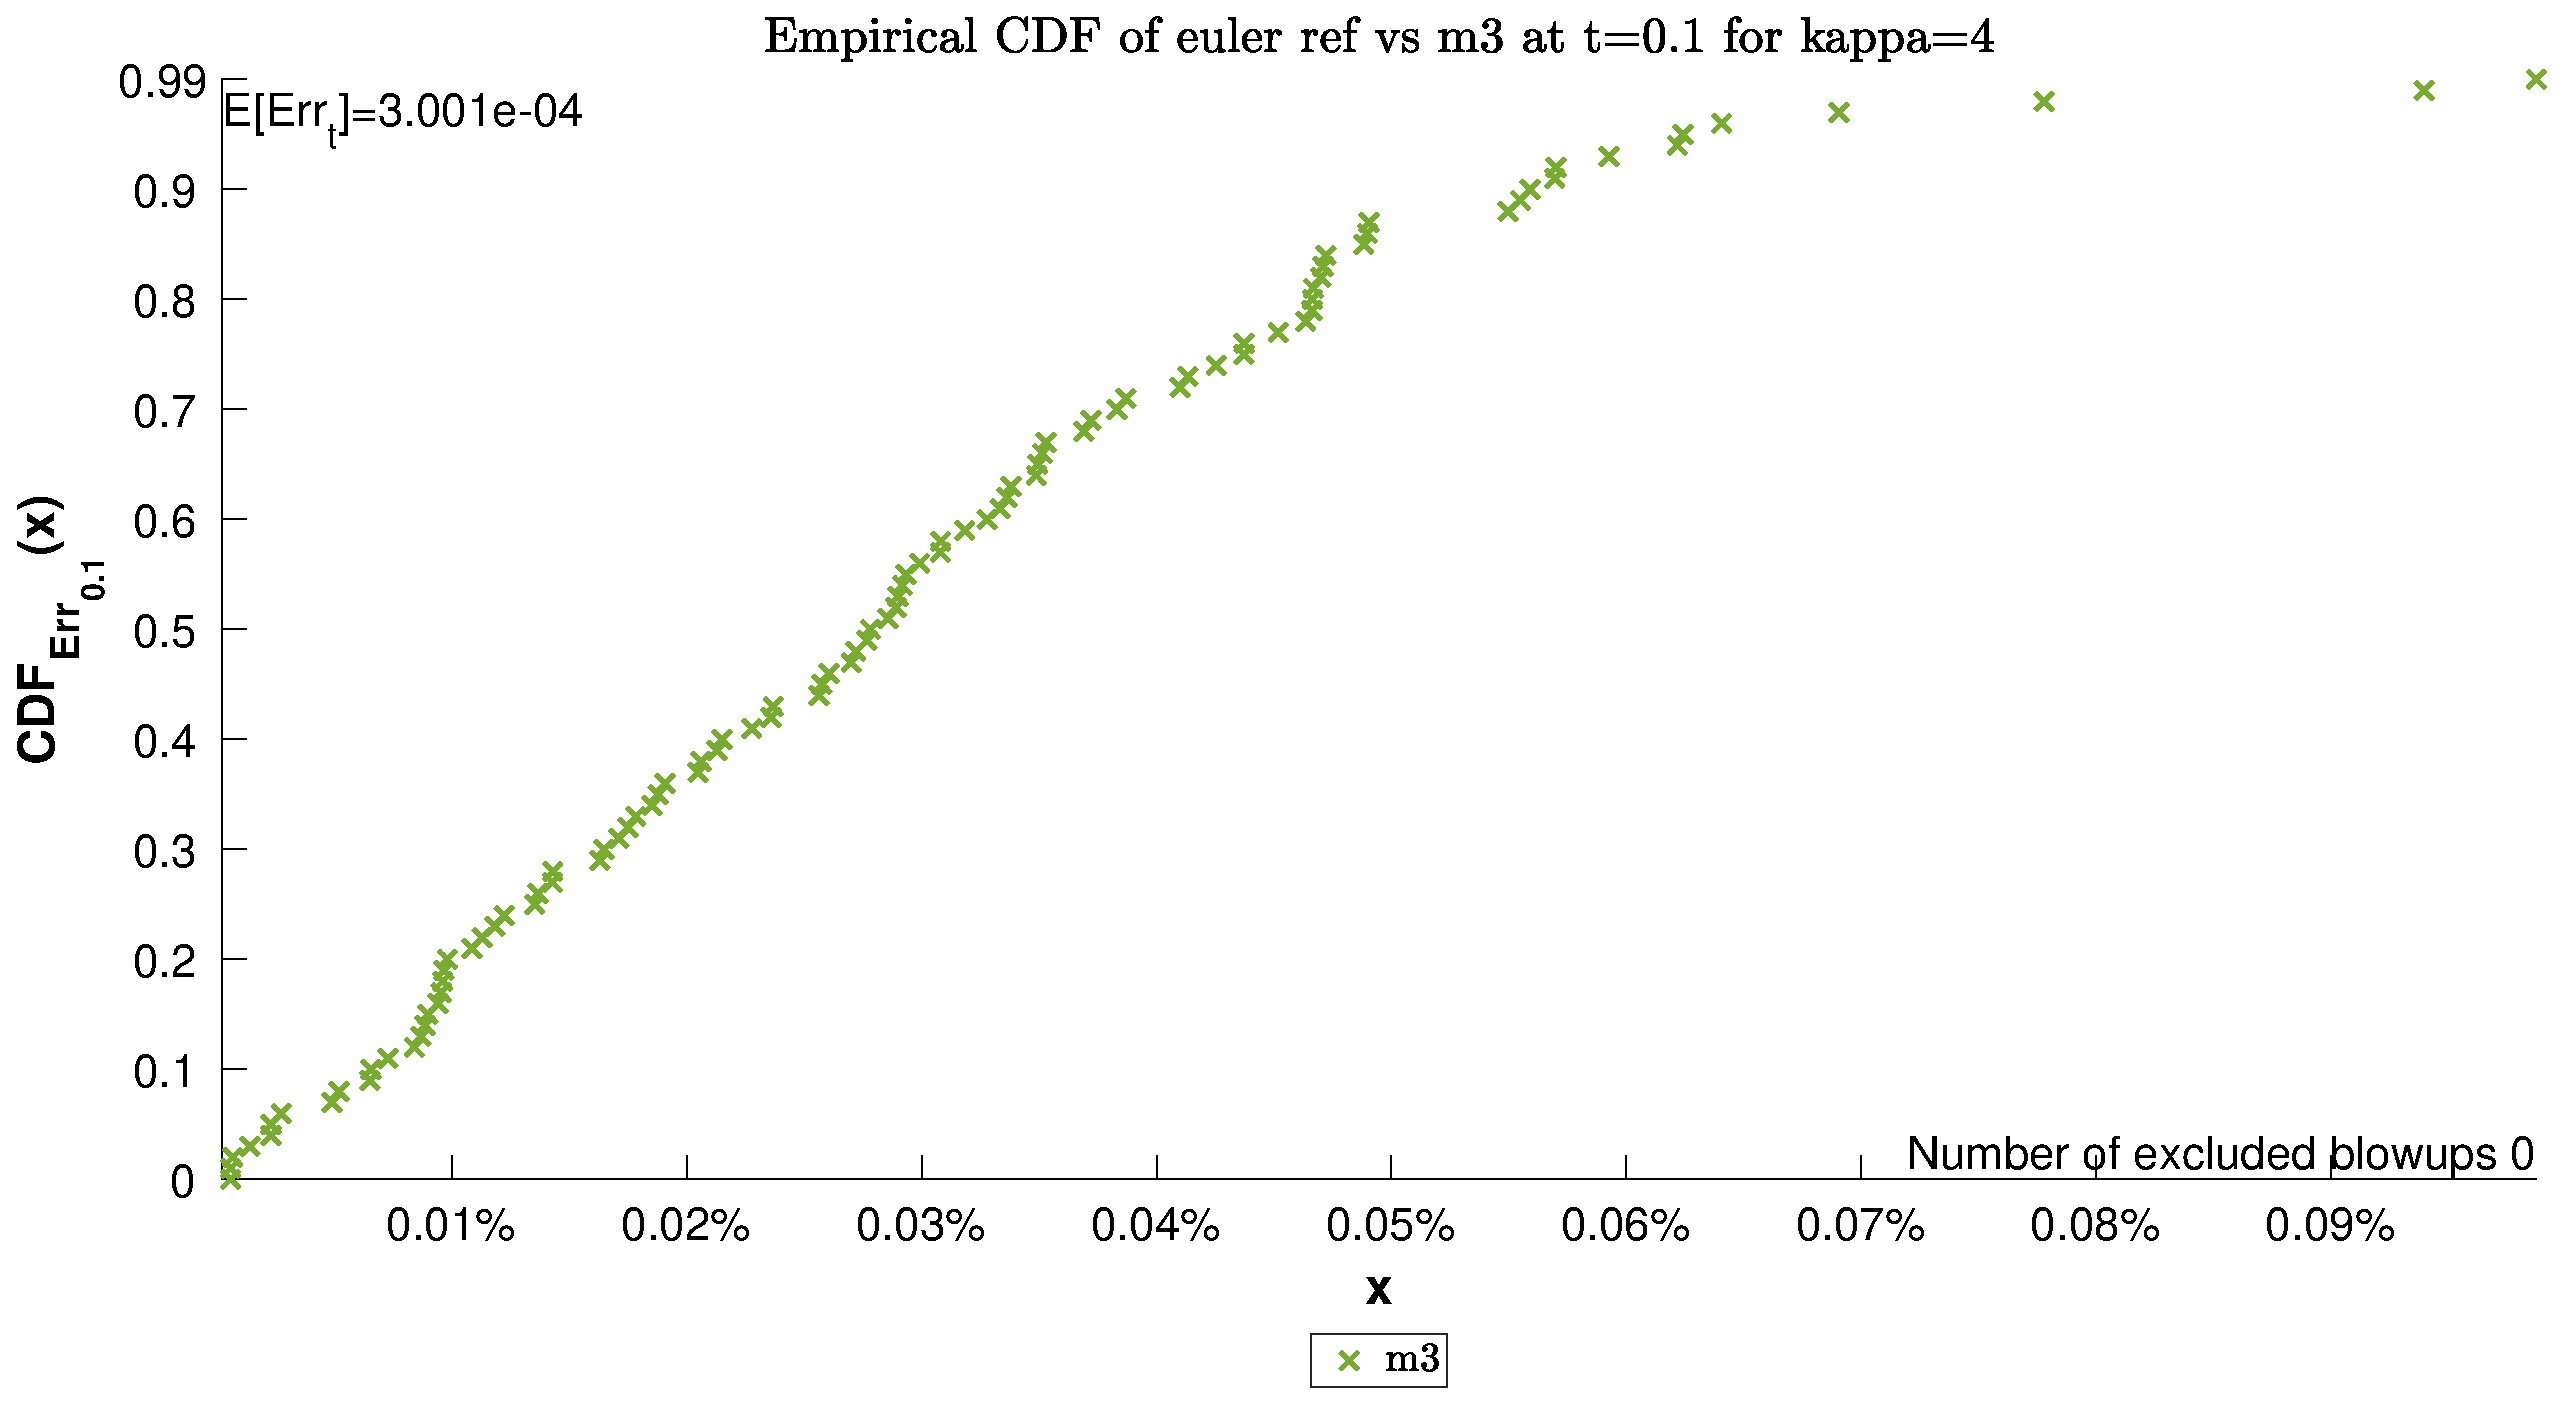
\includegraphics[width=.95\columnwidth]{CDF/CDFEulerRef_36}
\end{landscape}

\subsection{Sparsity Patterns}
	\begin{landscape}
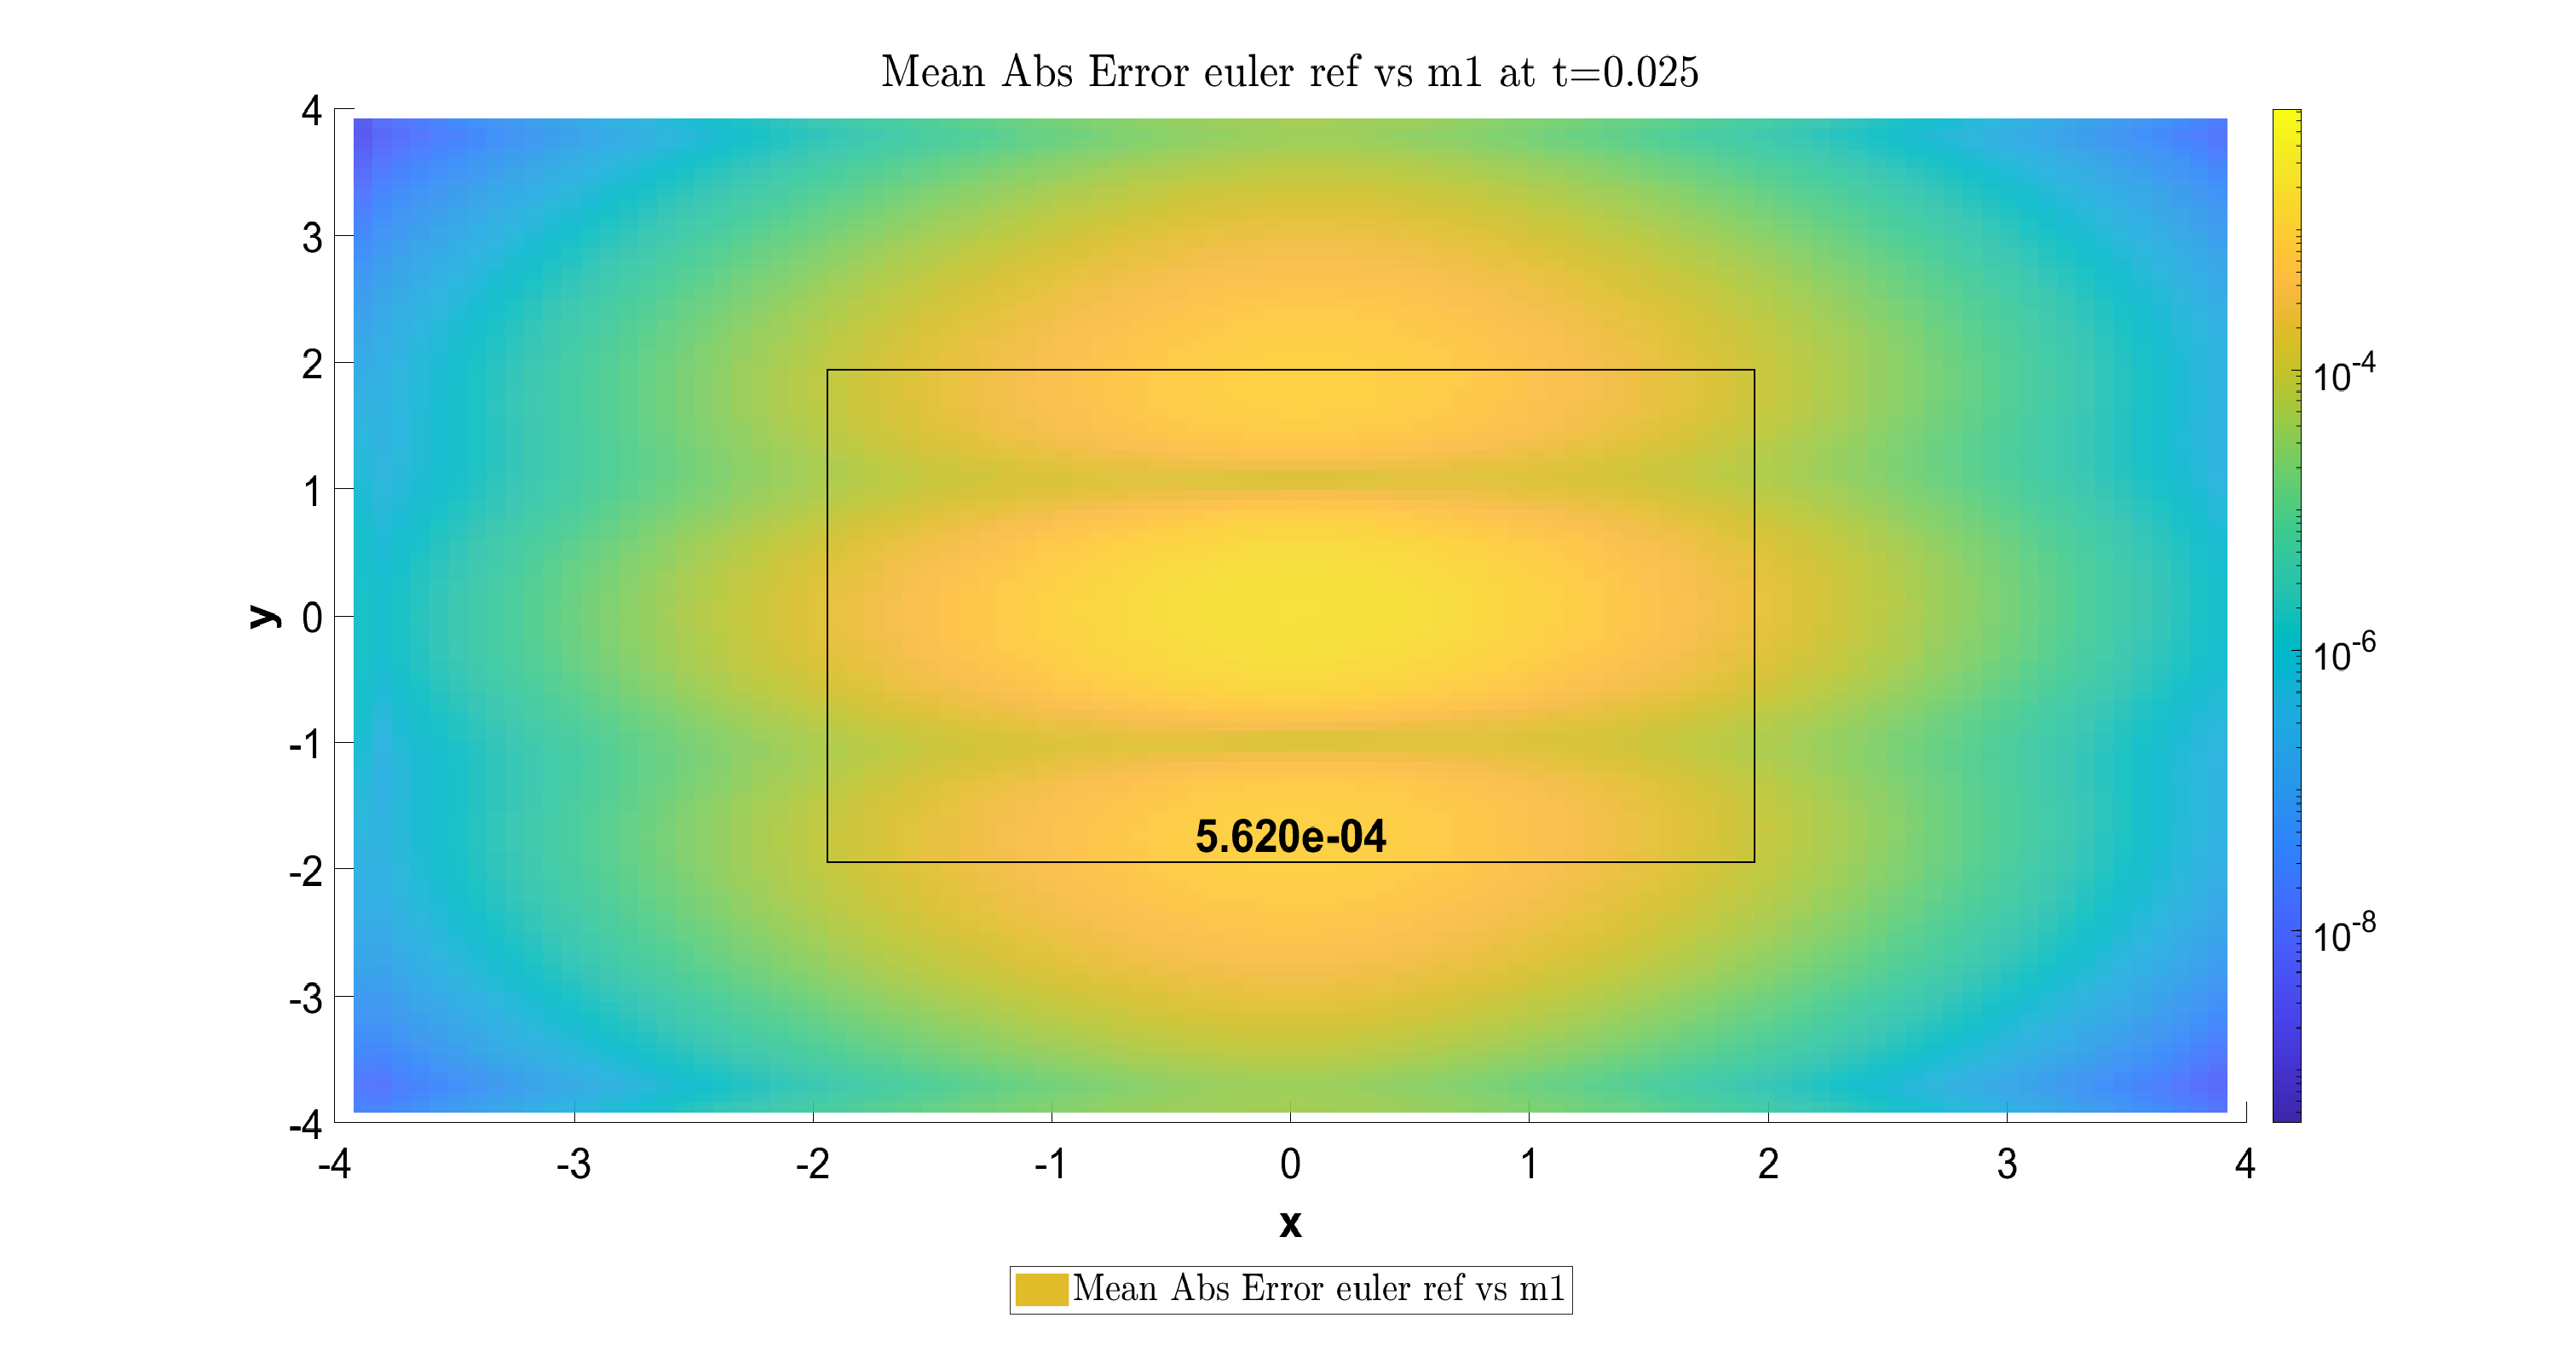
\includegraphics[width=.95\columnwidth]{CDF/CDFEulerRef_1}
\end{landscape}
\begin{landscape}
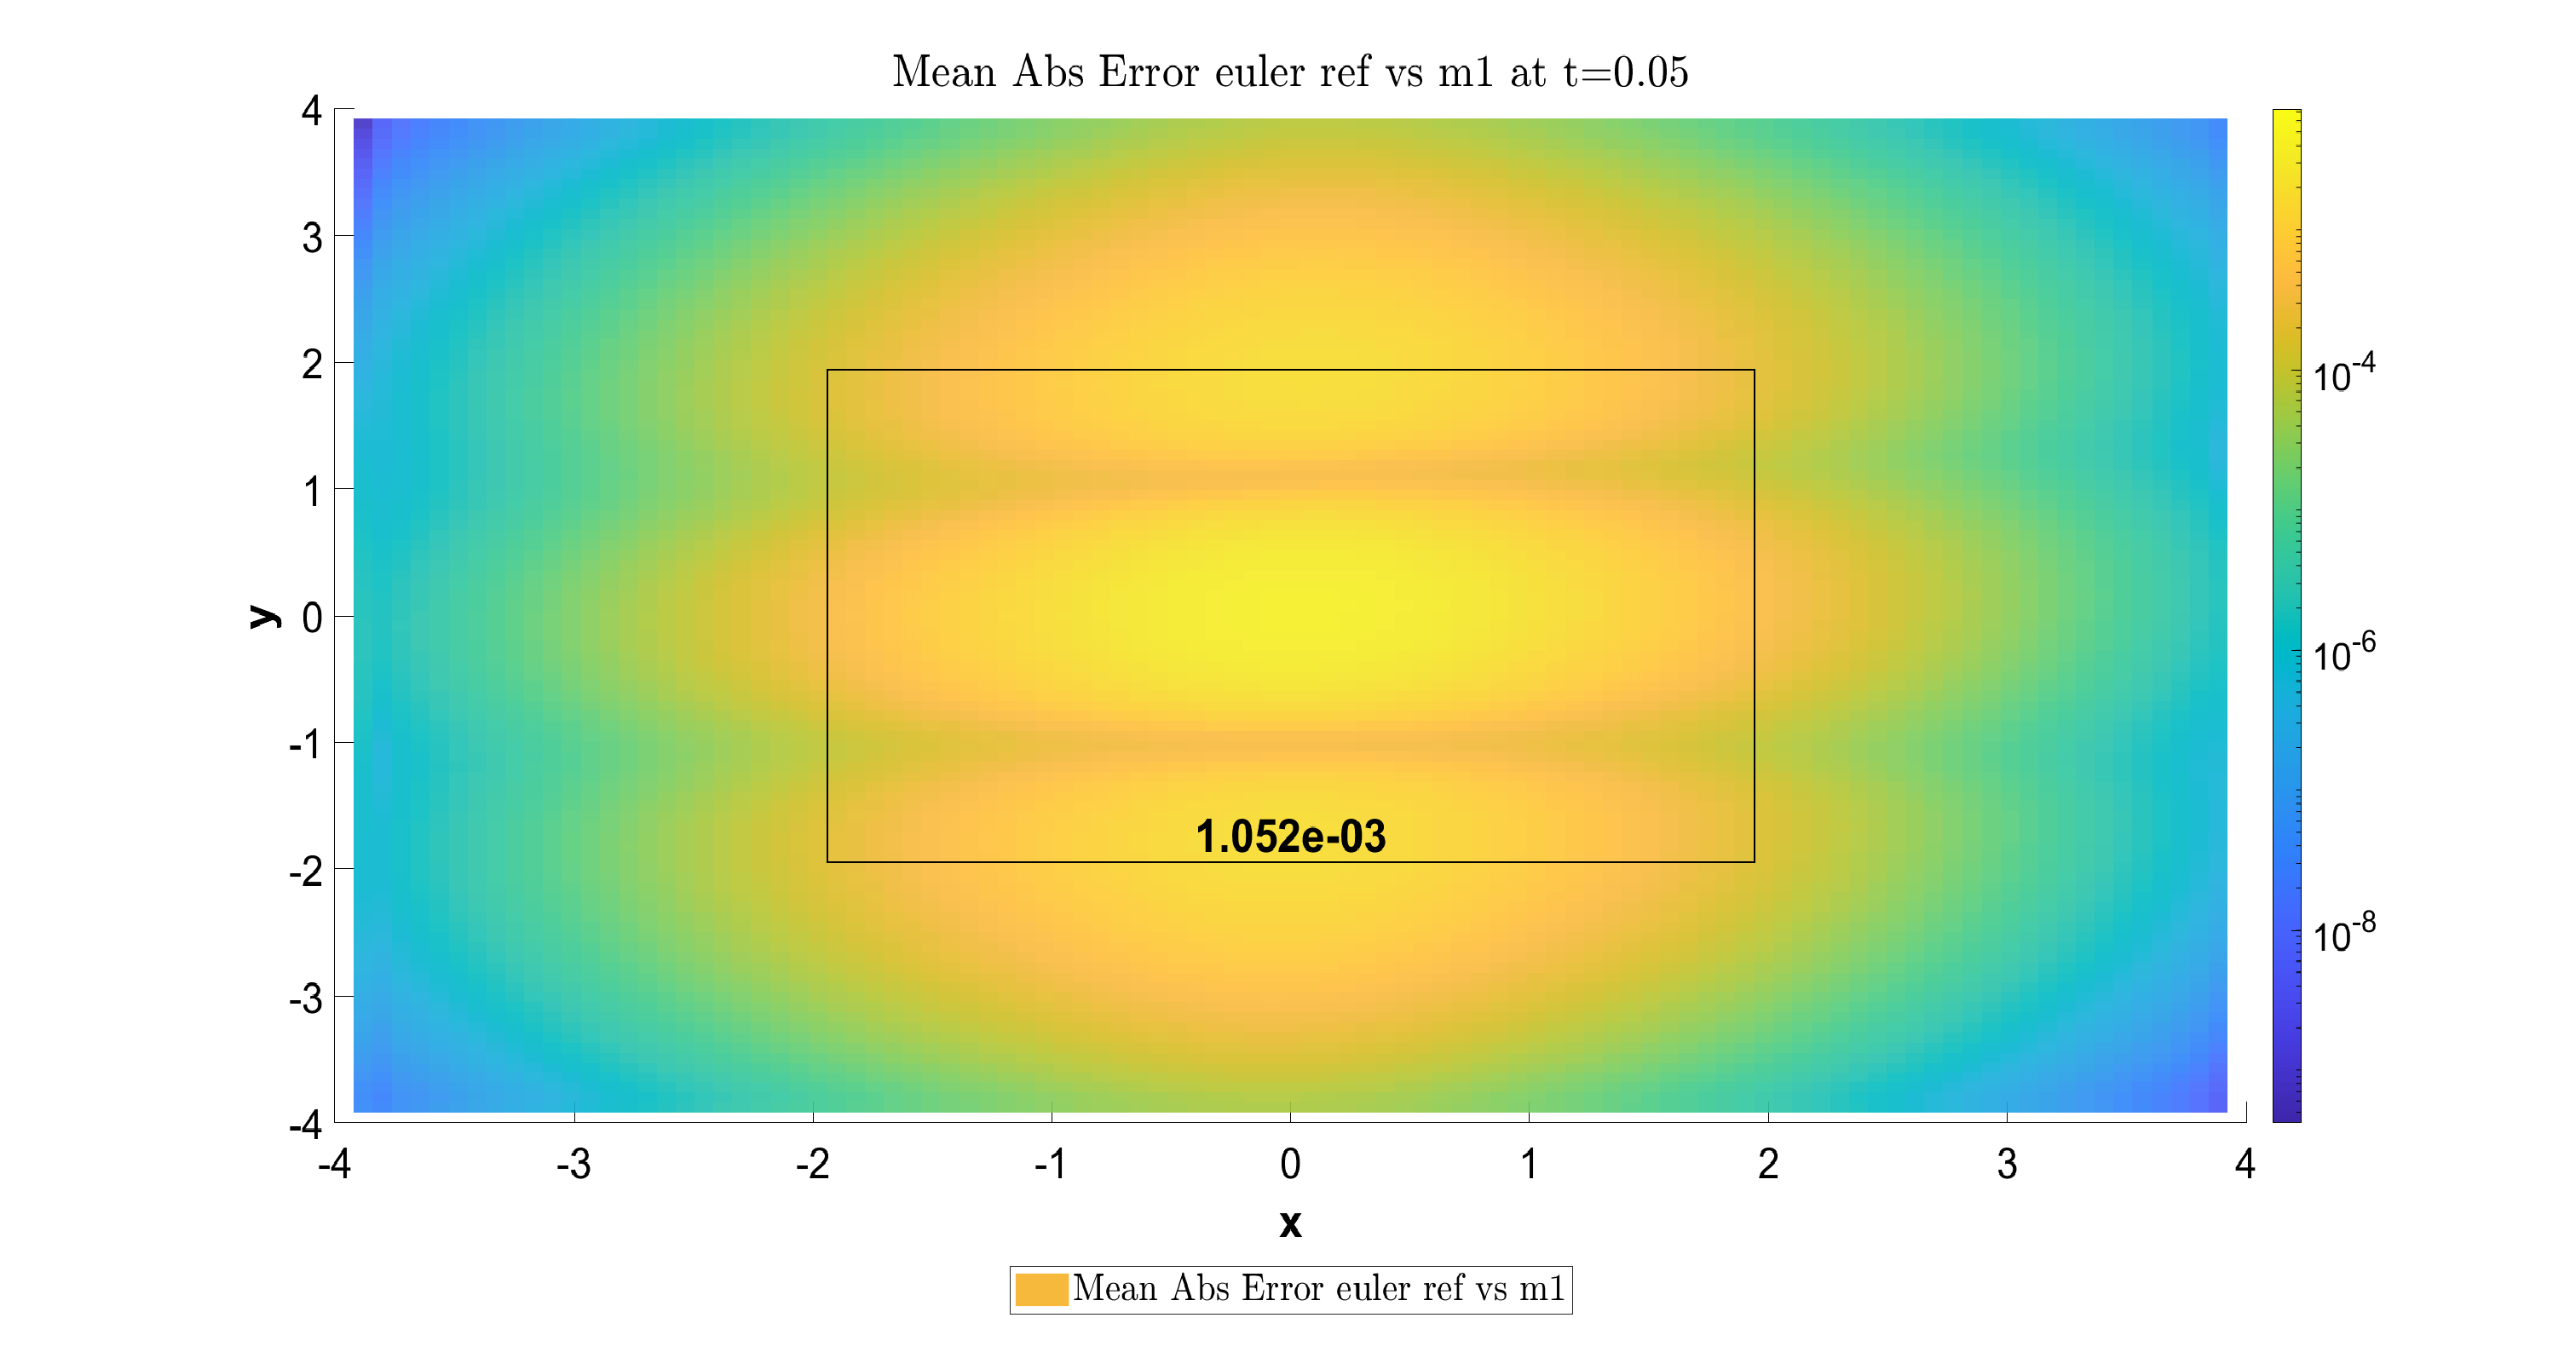
\includegraphics[width=.95\columnwidth]{CDF/CDFEulerRef_2}
\end{landscape}
\begin{landscape}
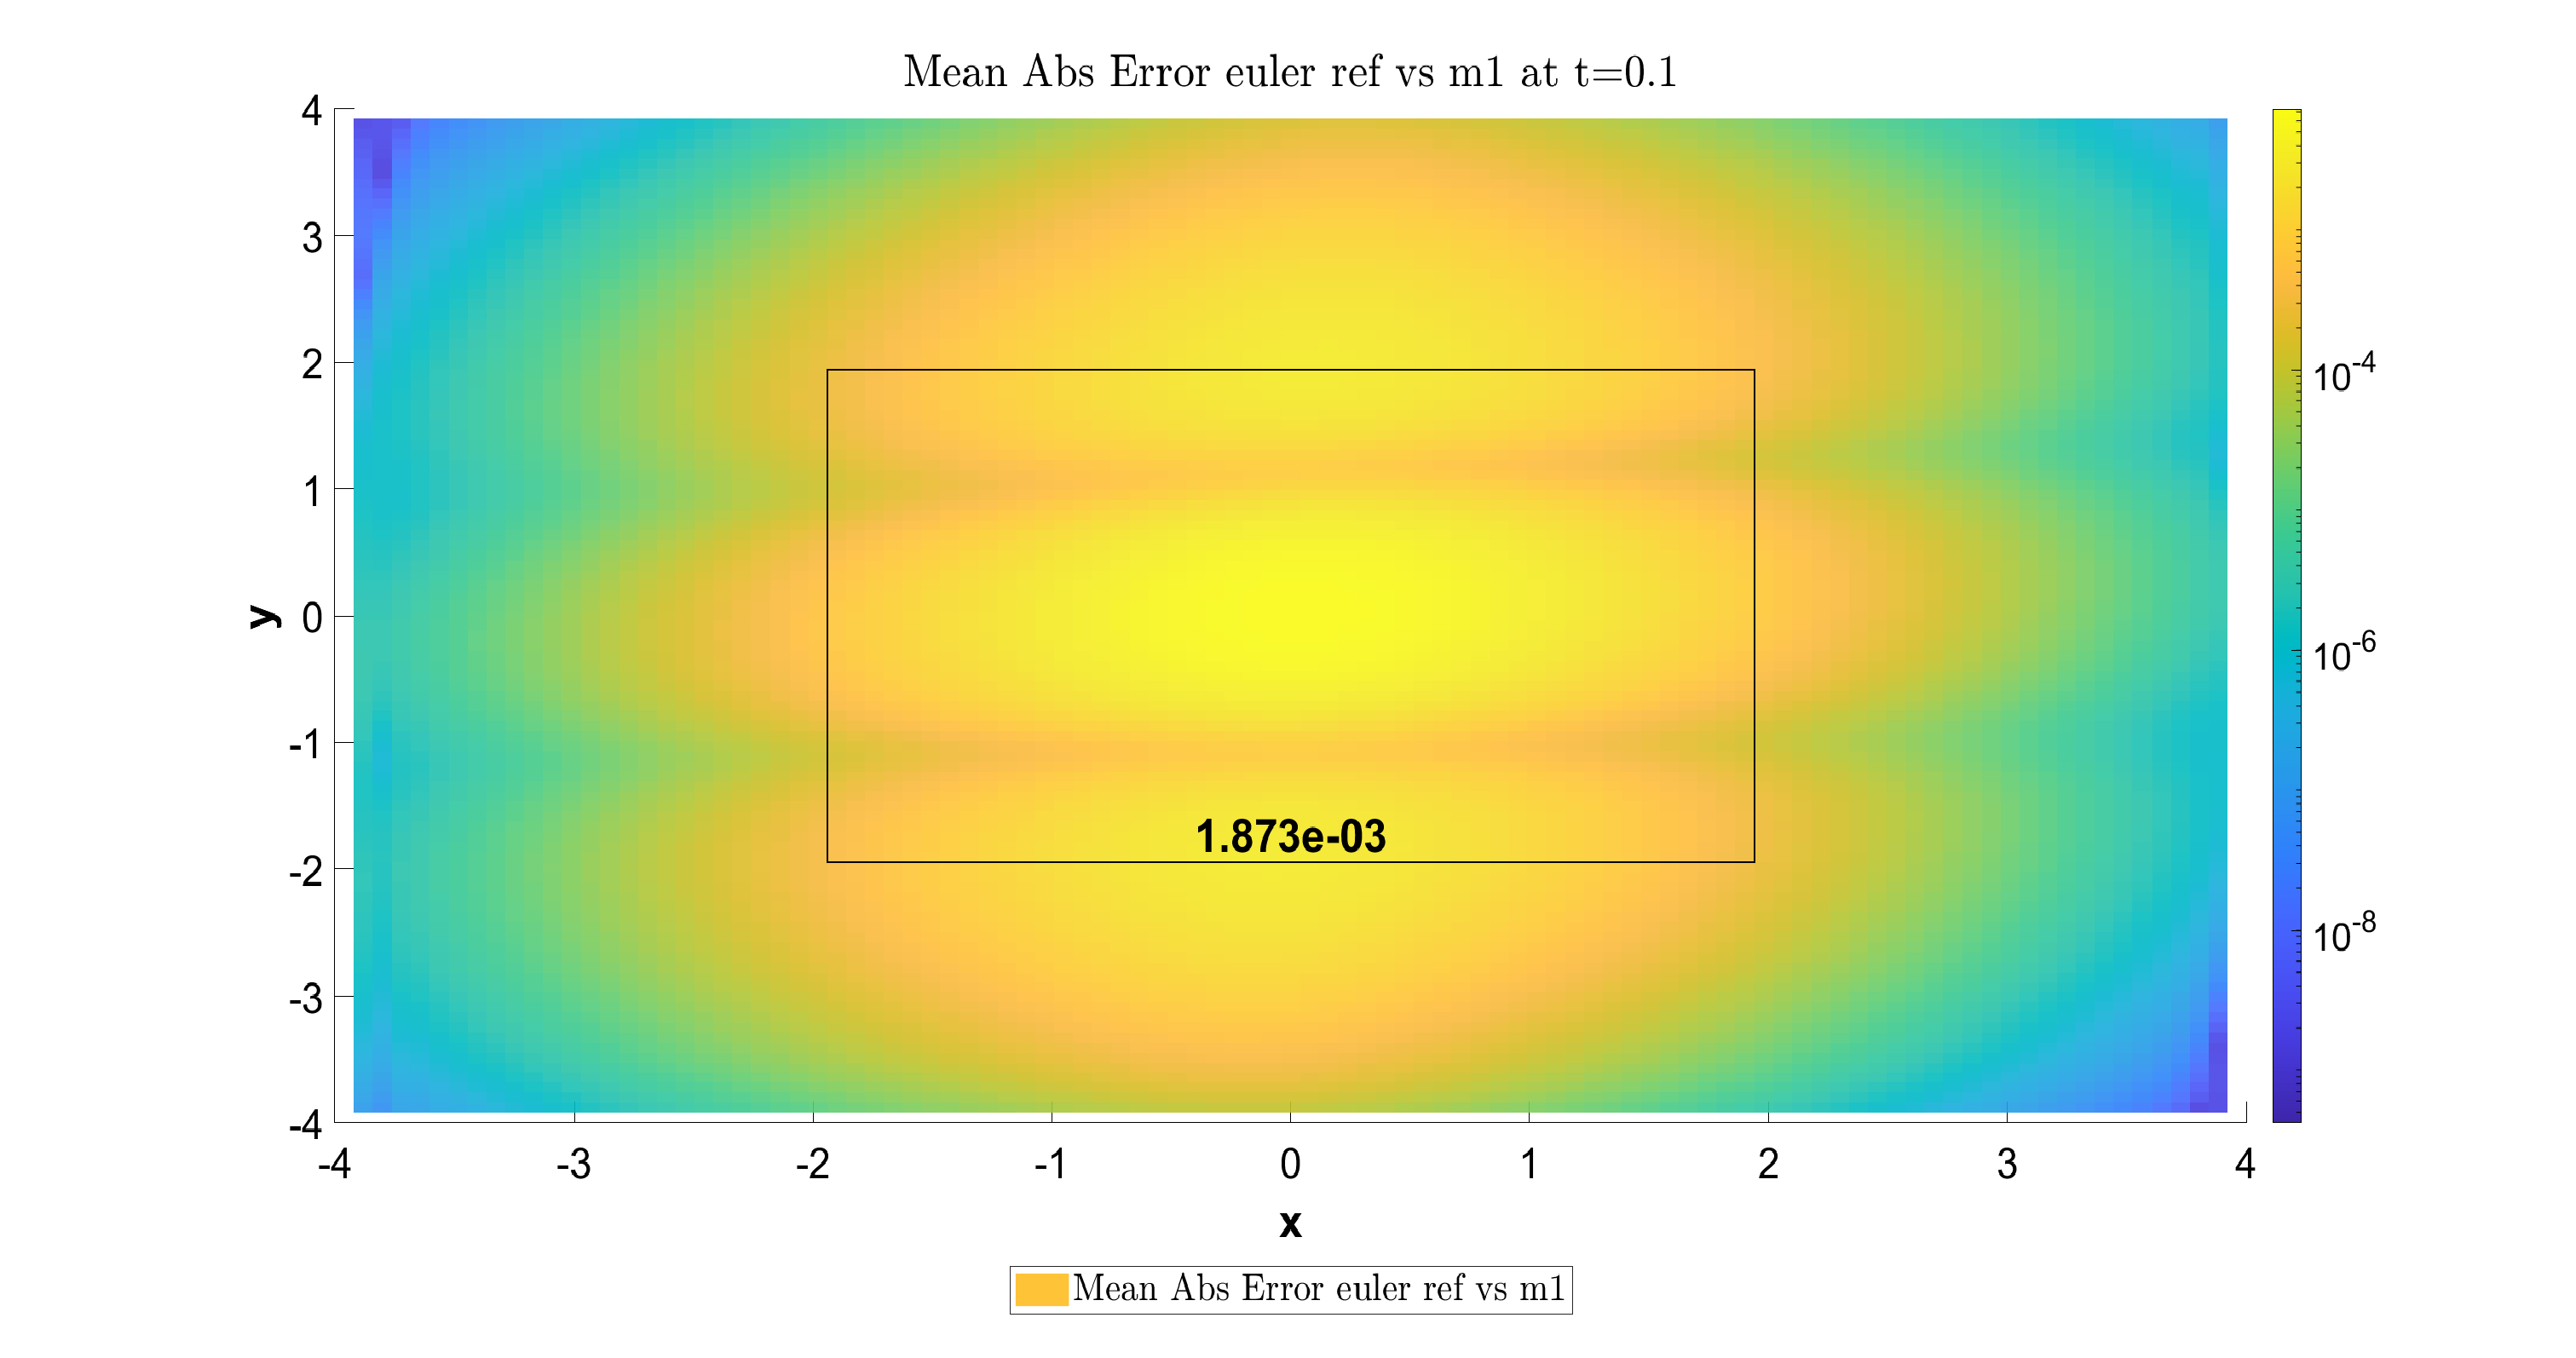
\includegraphics[width=.95\columnwidth]{CDF/CDFEulerRef_3}
\end{landscape}
\begin{landscape}
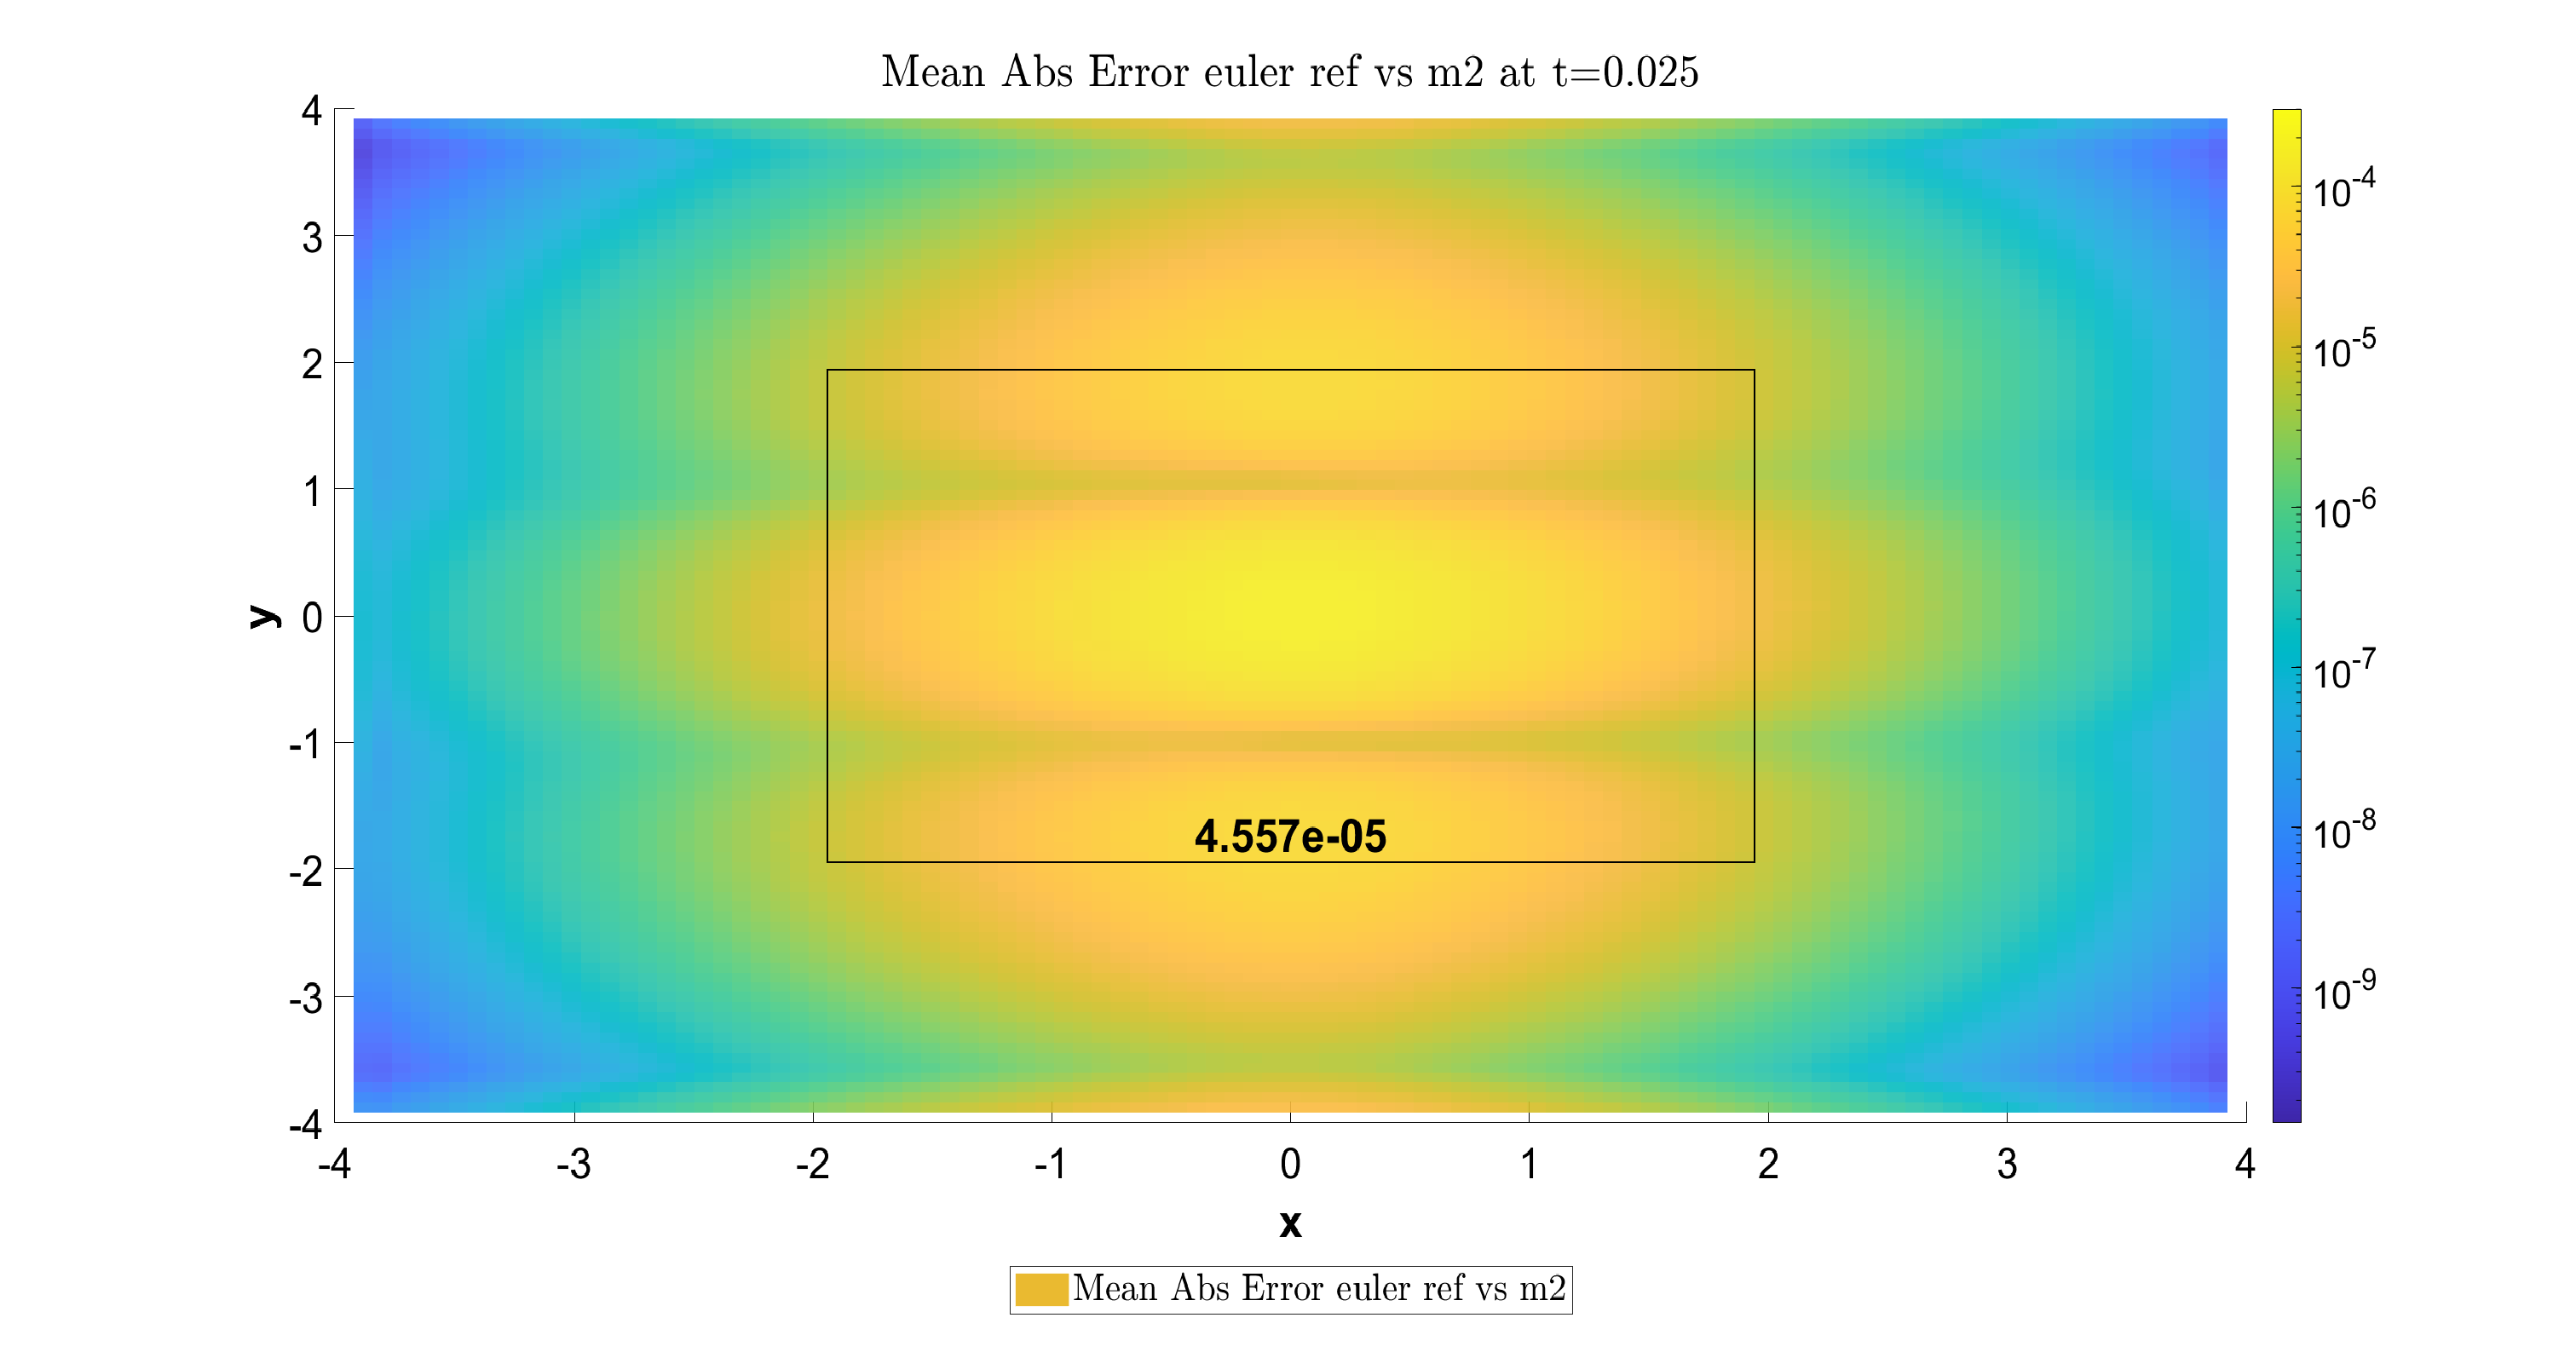
\includegraphics[width=.95\columnwidth]{CDF/CDFEulerRef_4}
\end{landscape}
\begin{landscape}
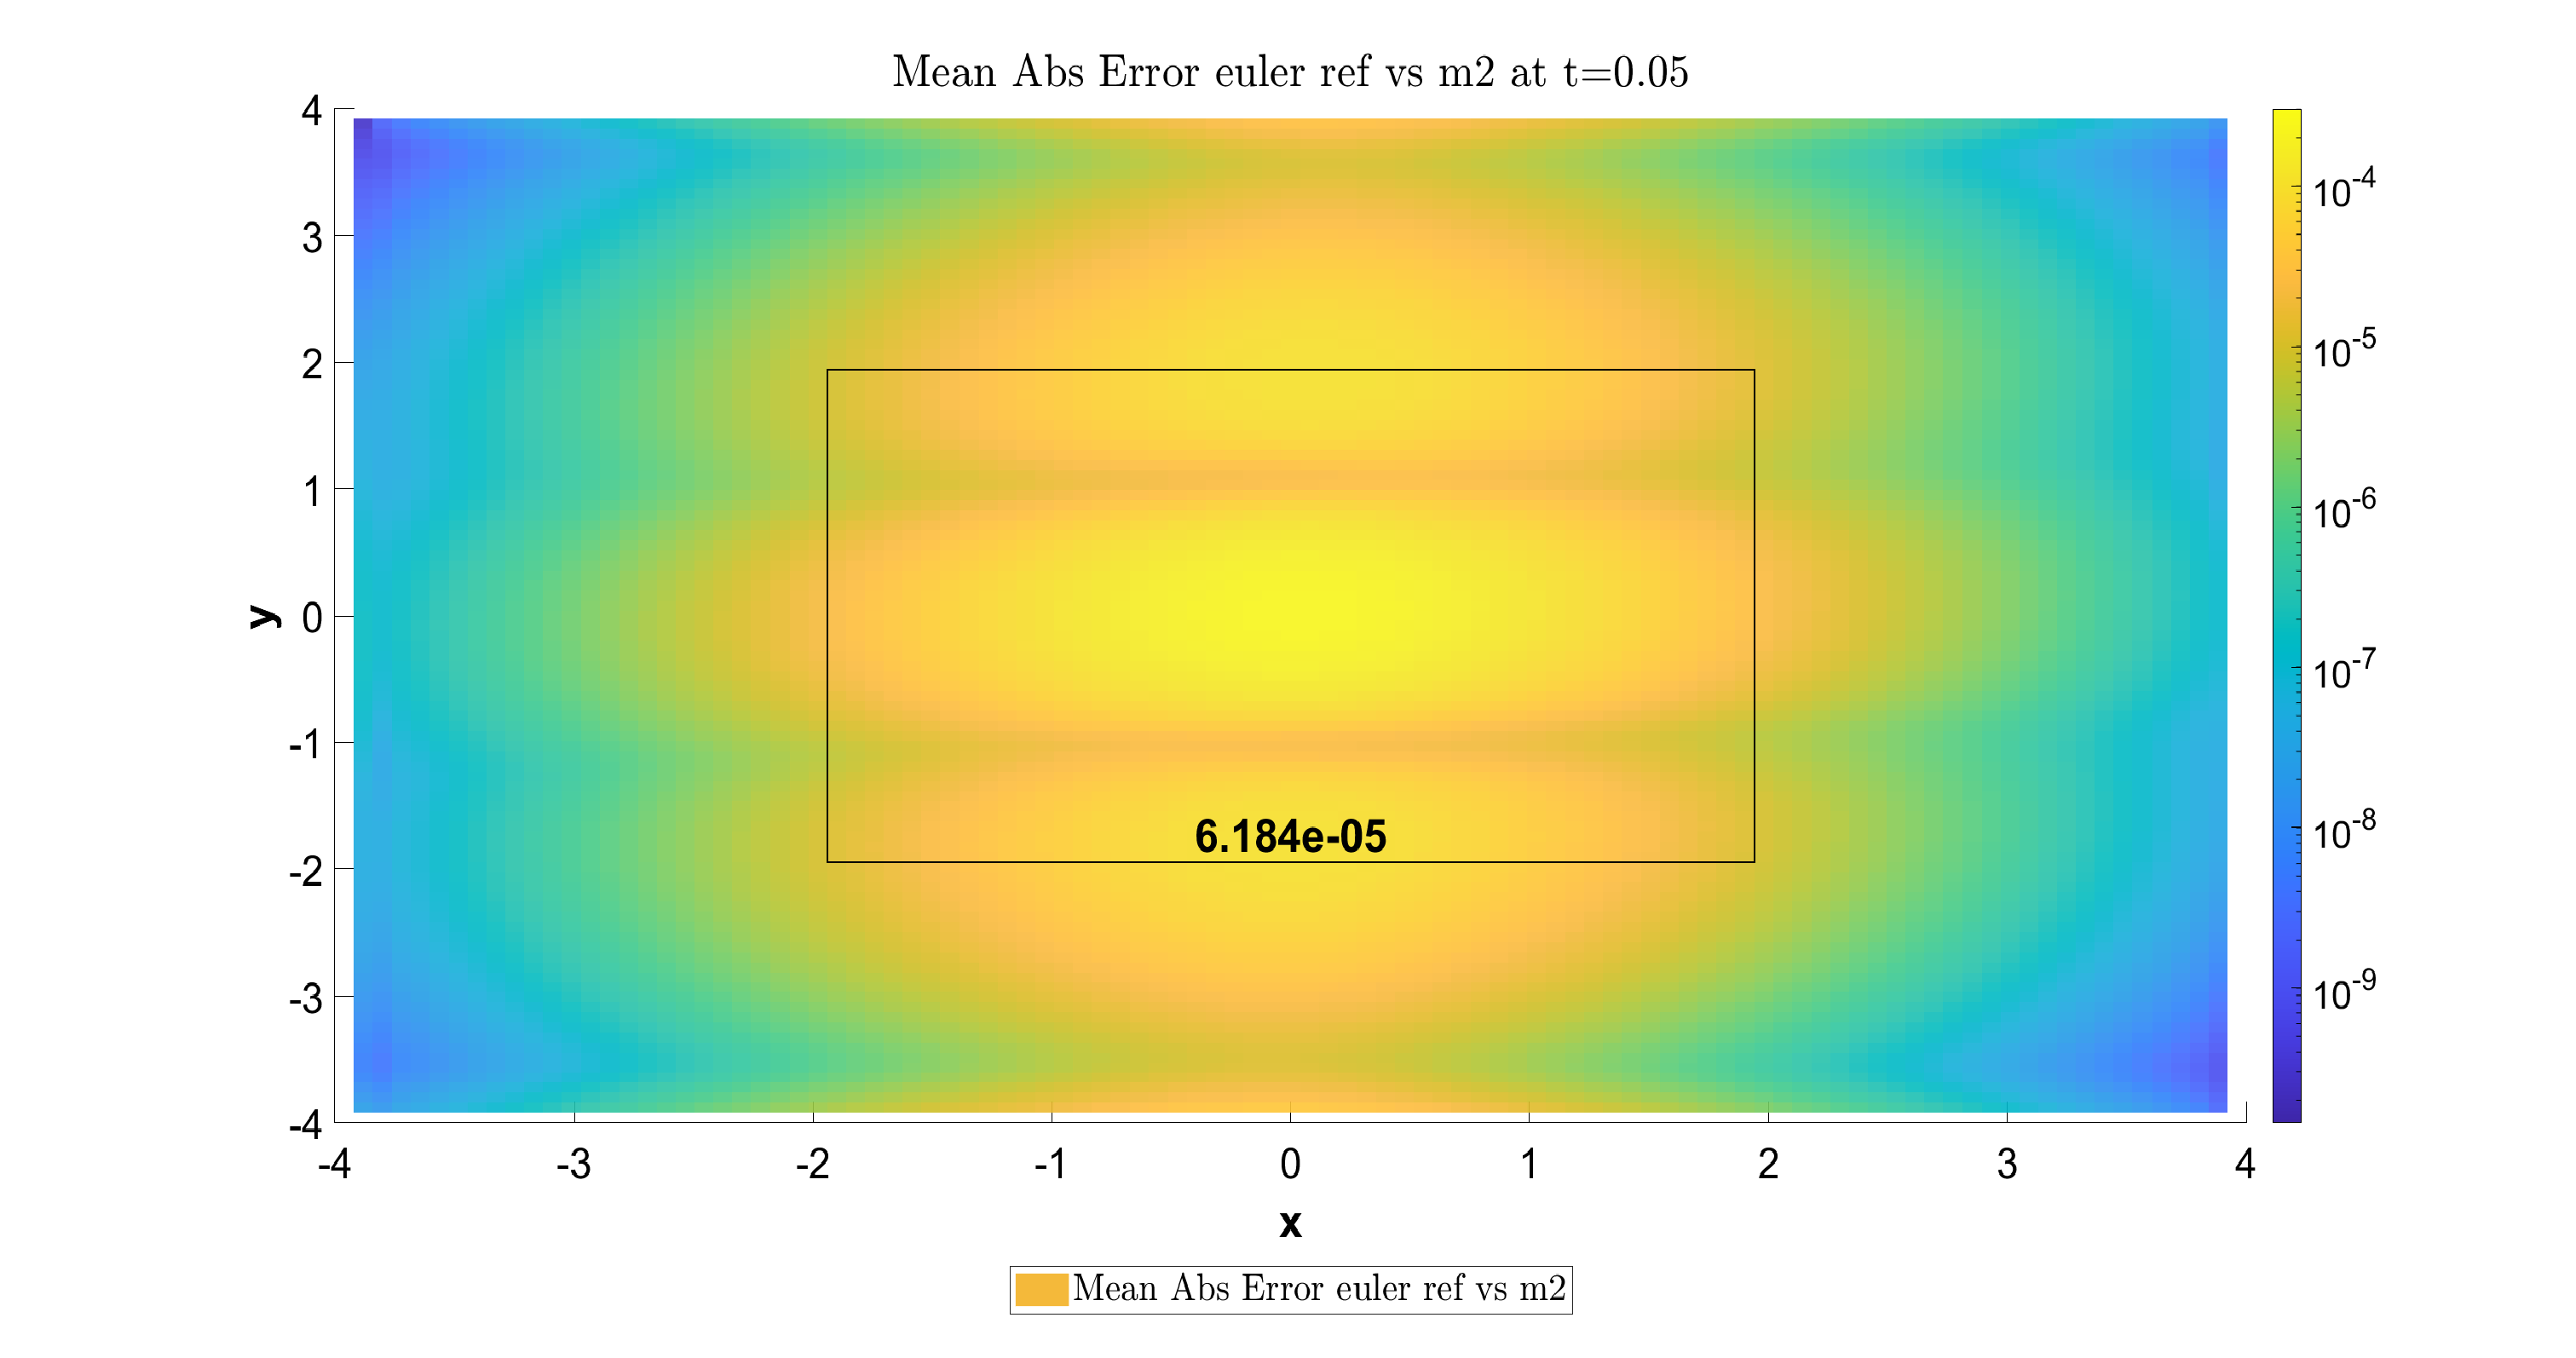
\includegraphics[width=.95\columnwidth]{CDF/CDFEulerRef_5}
\end{landscape}
\begin{landscape}
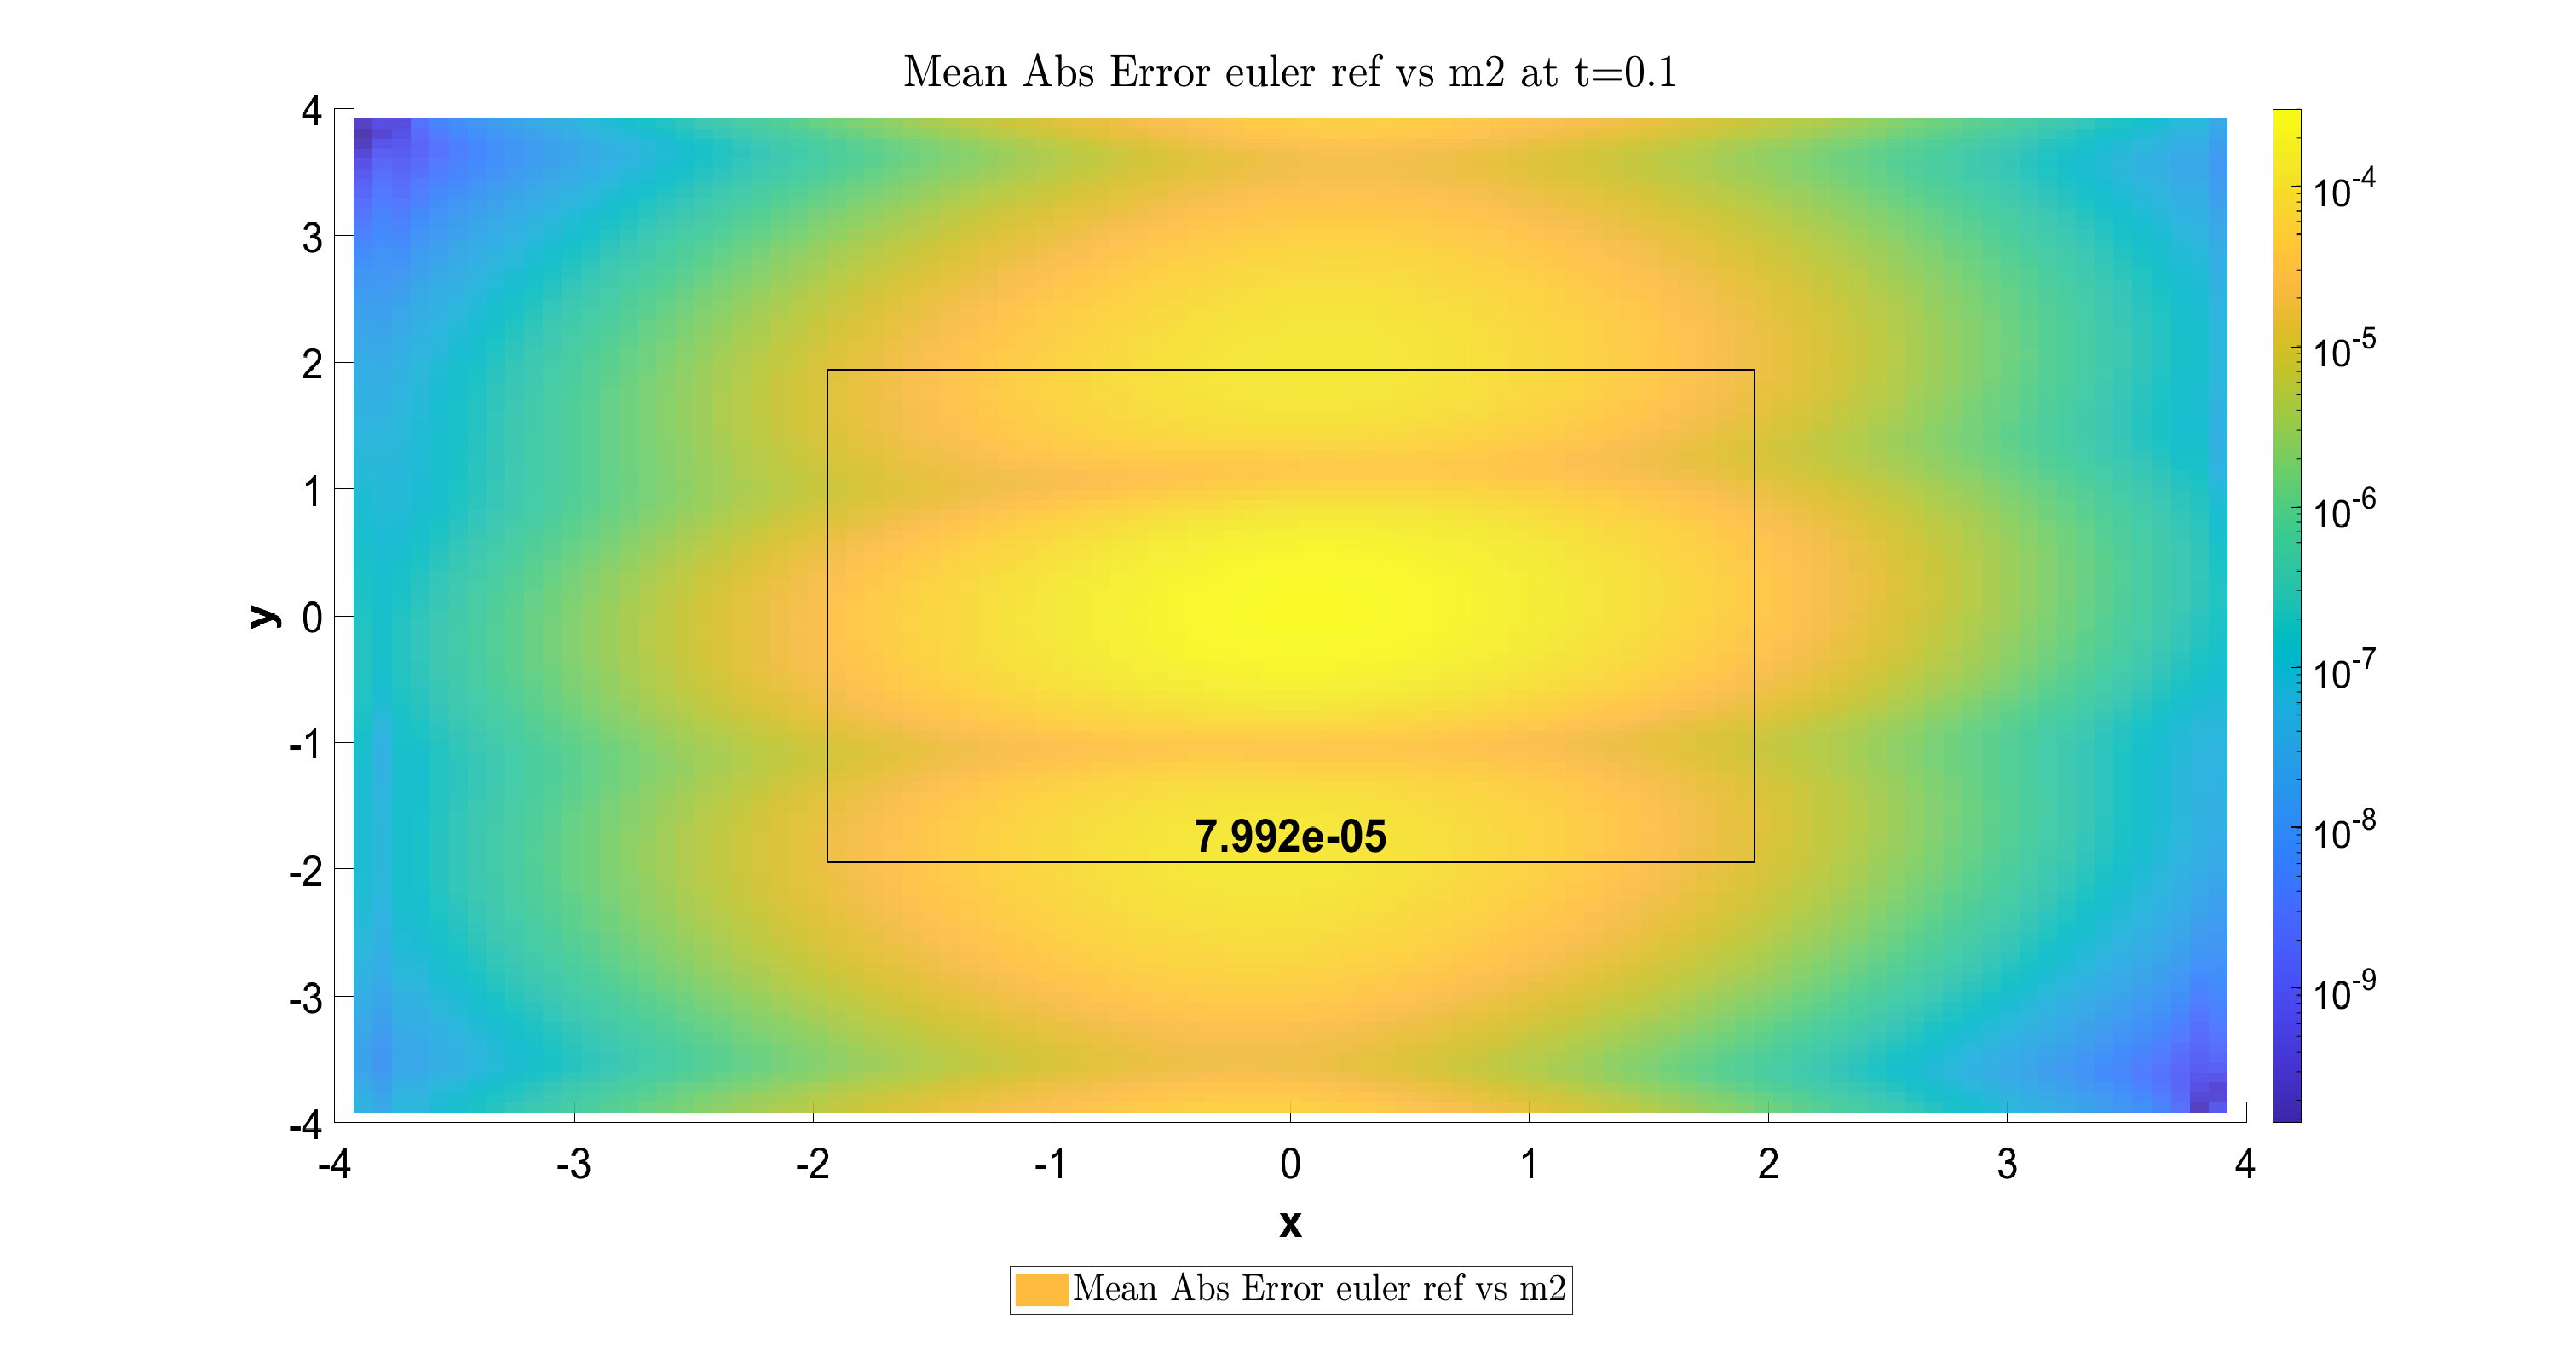
\includegraphics[width=.95\columnwidth]{CDF/CDFEulerRef_6}
\end{landscape}
\begin{landscape}
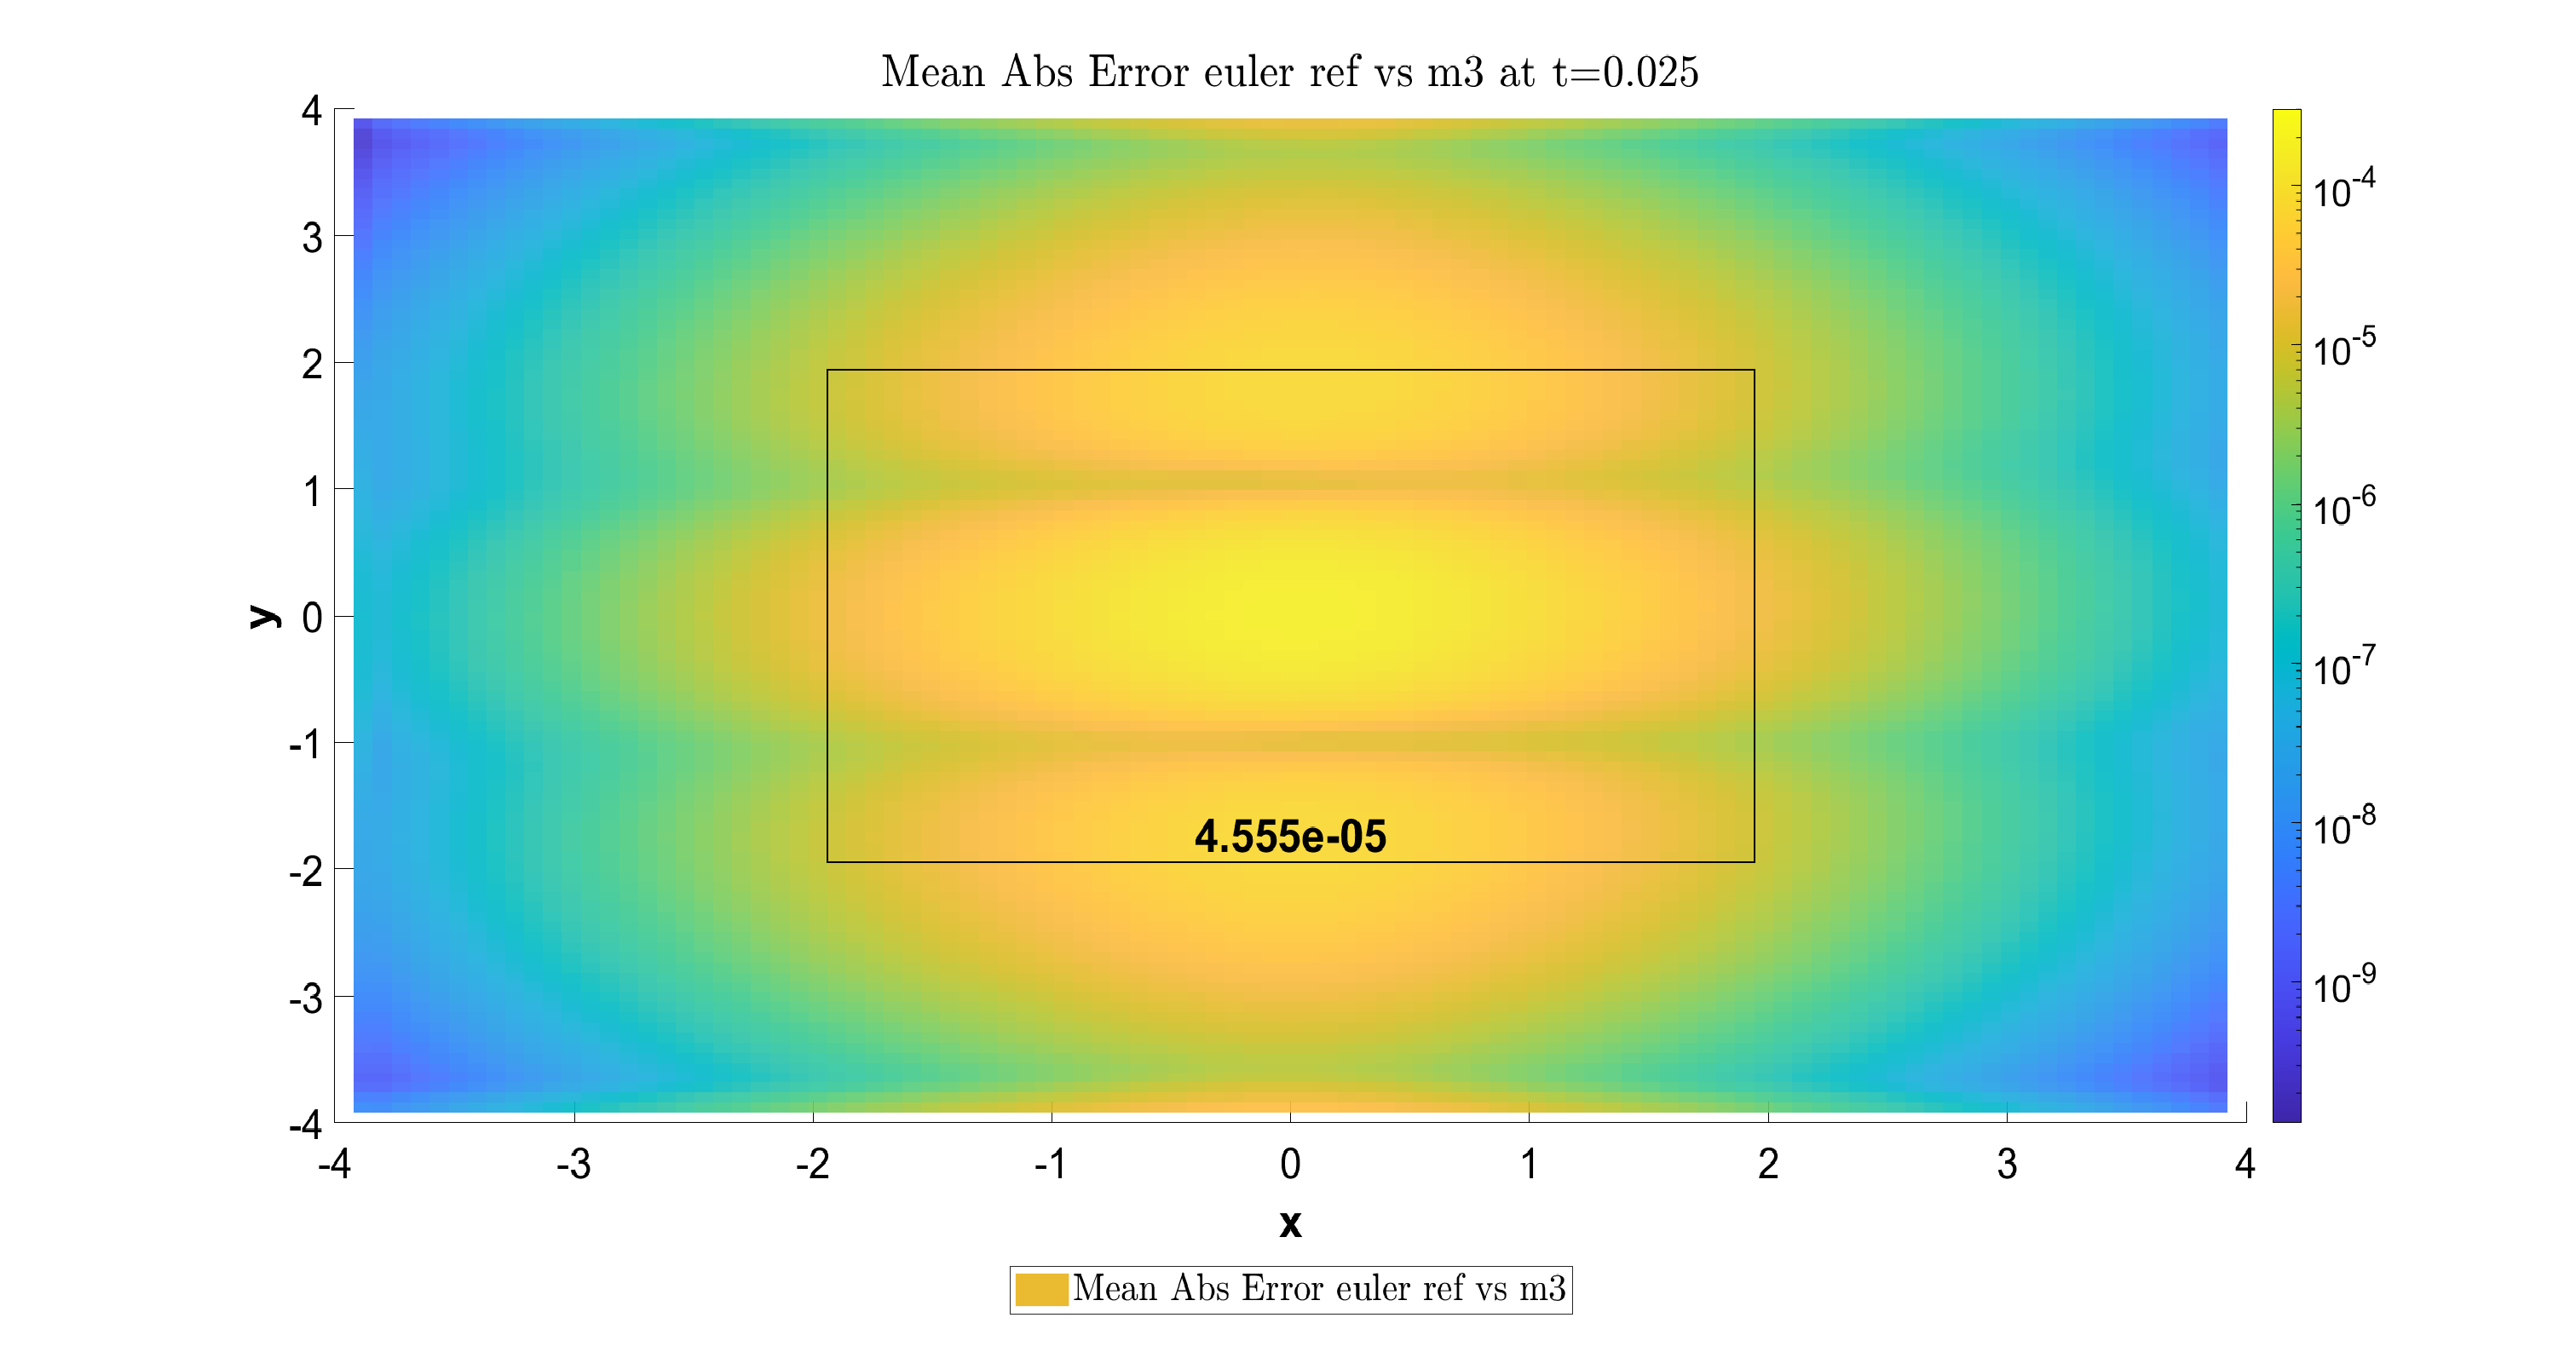
\includegraphics[width=.95\columnwidth]{CDF/CDFEulerRef_7}
\end{landscape}
\begin{landscape}
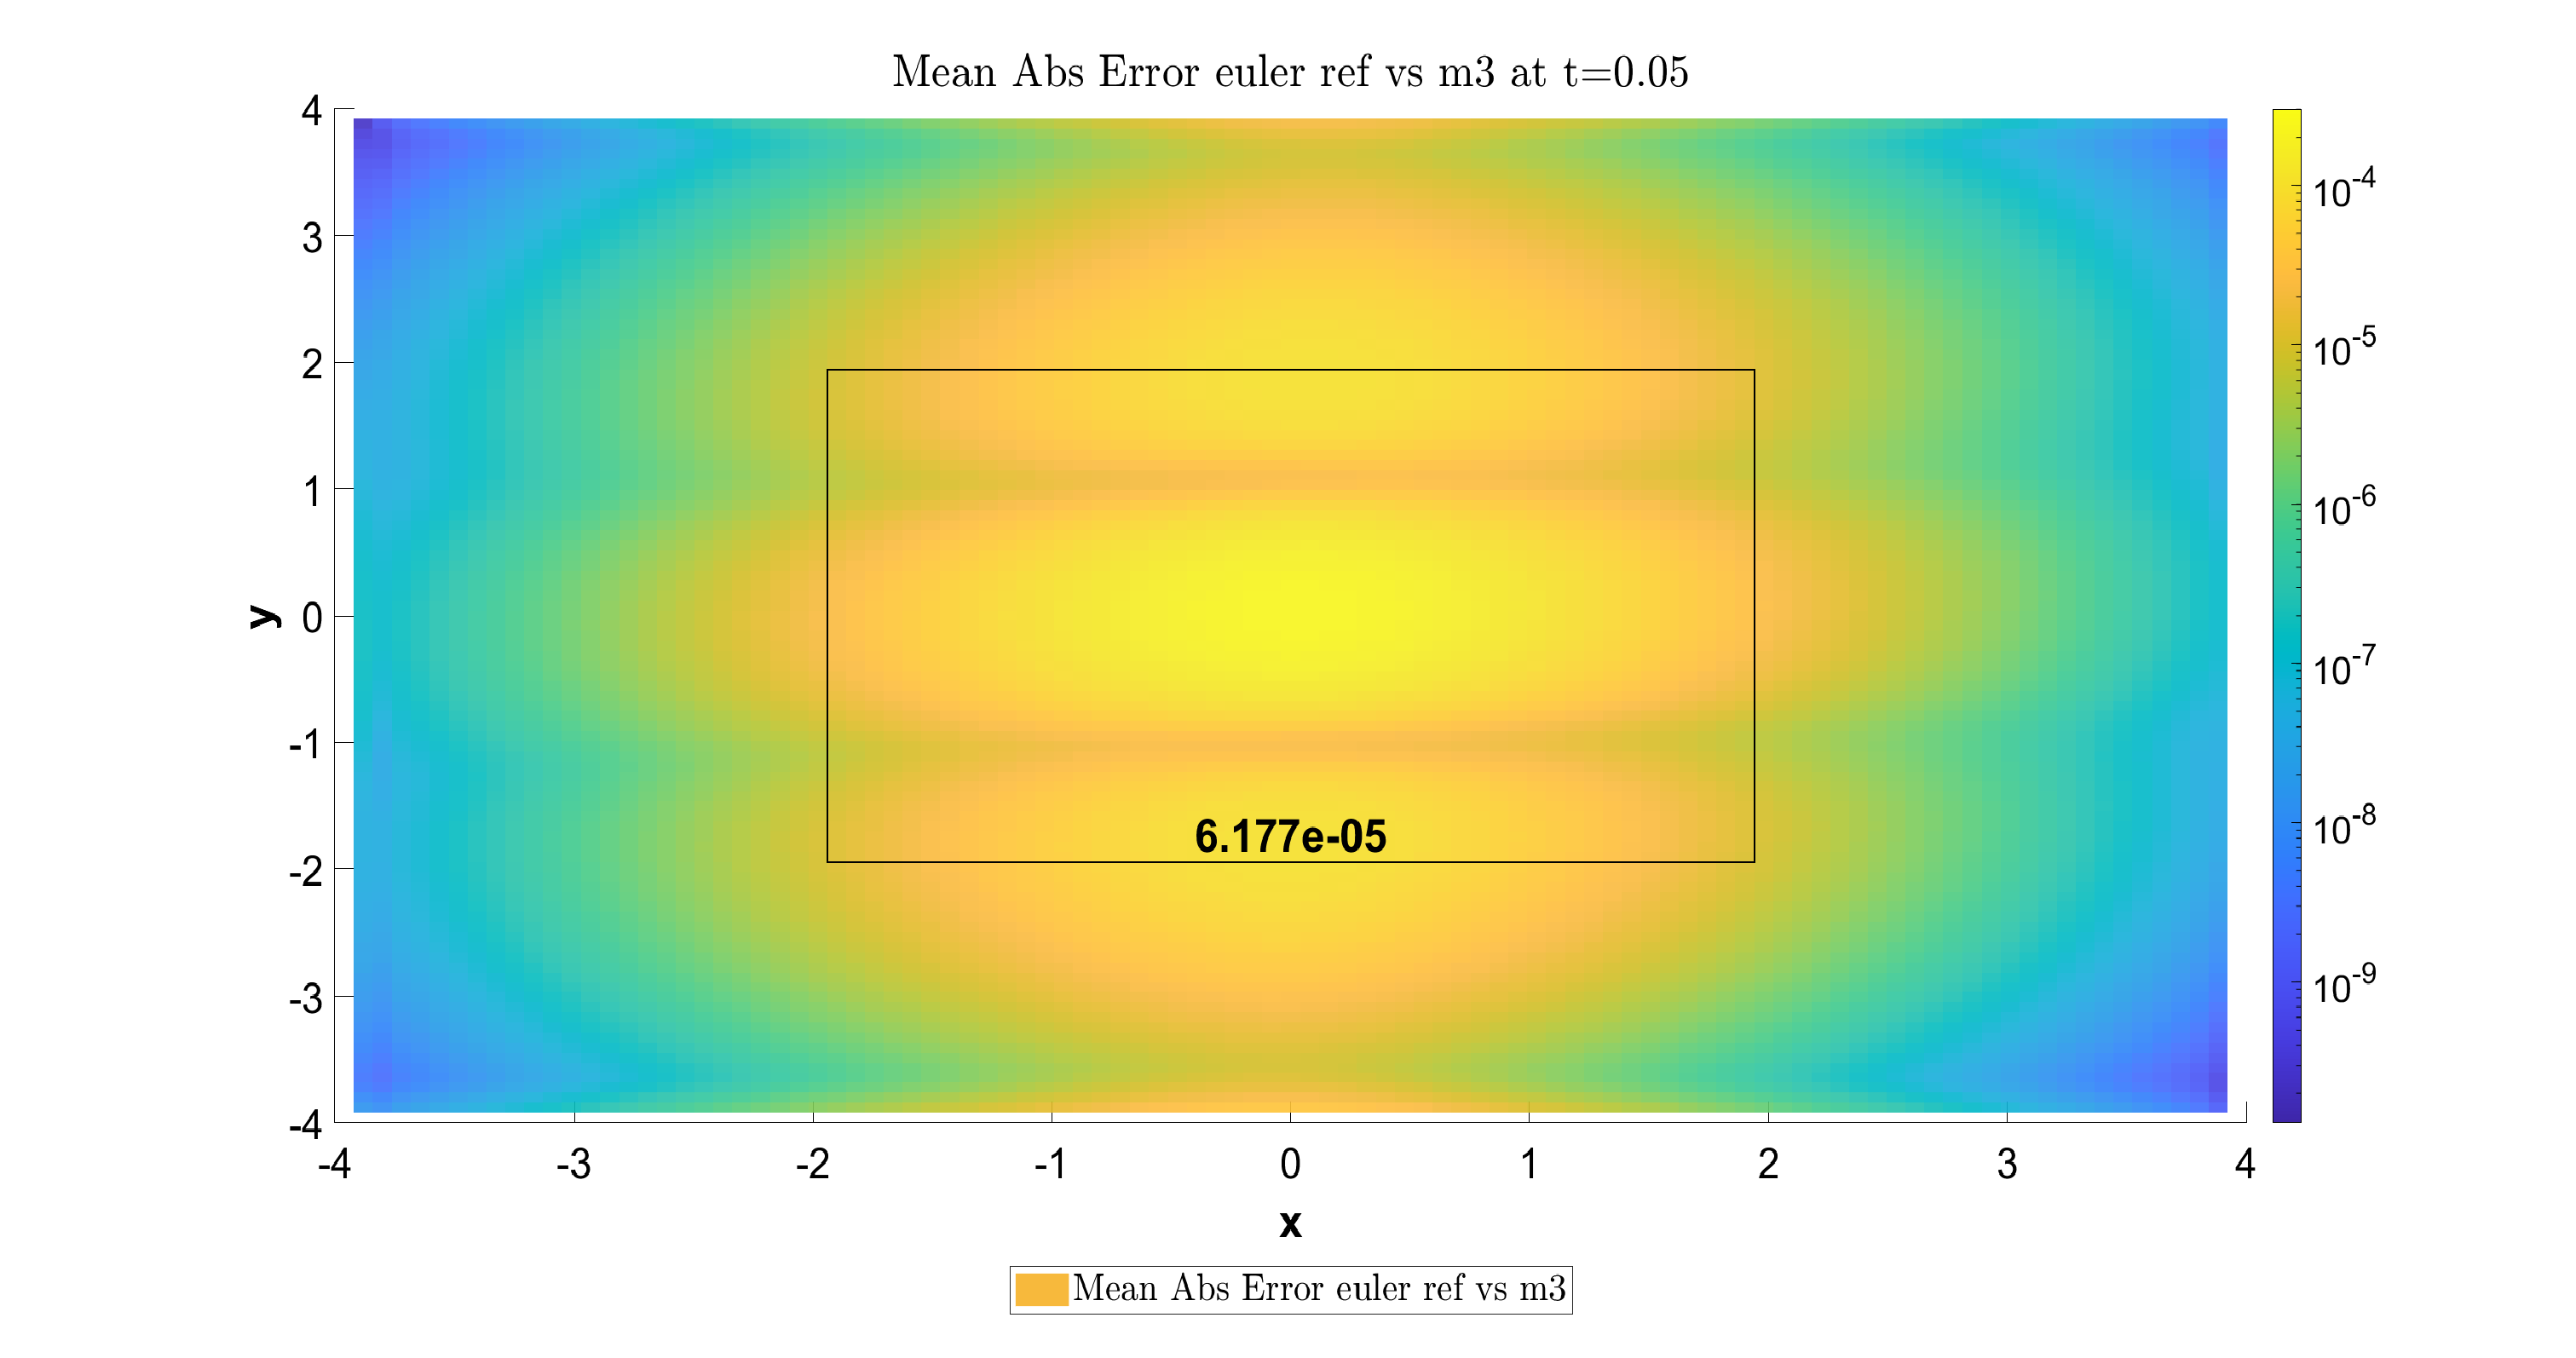
\includegraphics[width=.95\columnwidth]{CDF/CDFEulerRef_8}
\end{landscape}
\begin{landscape}
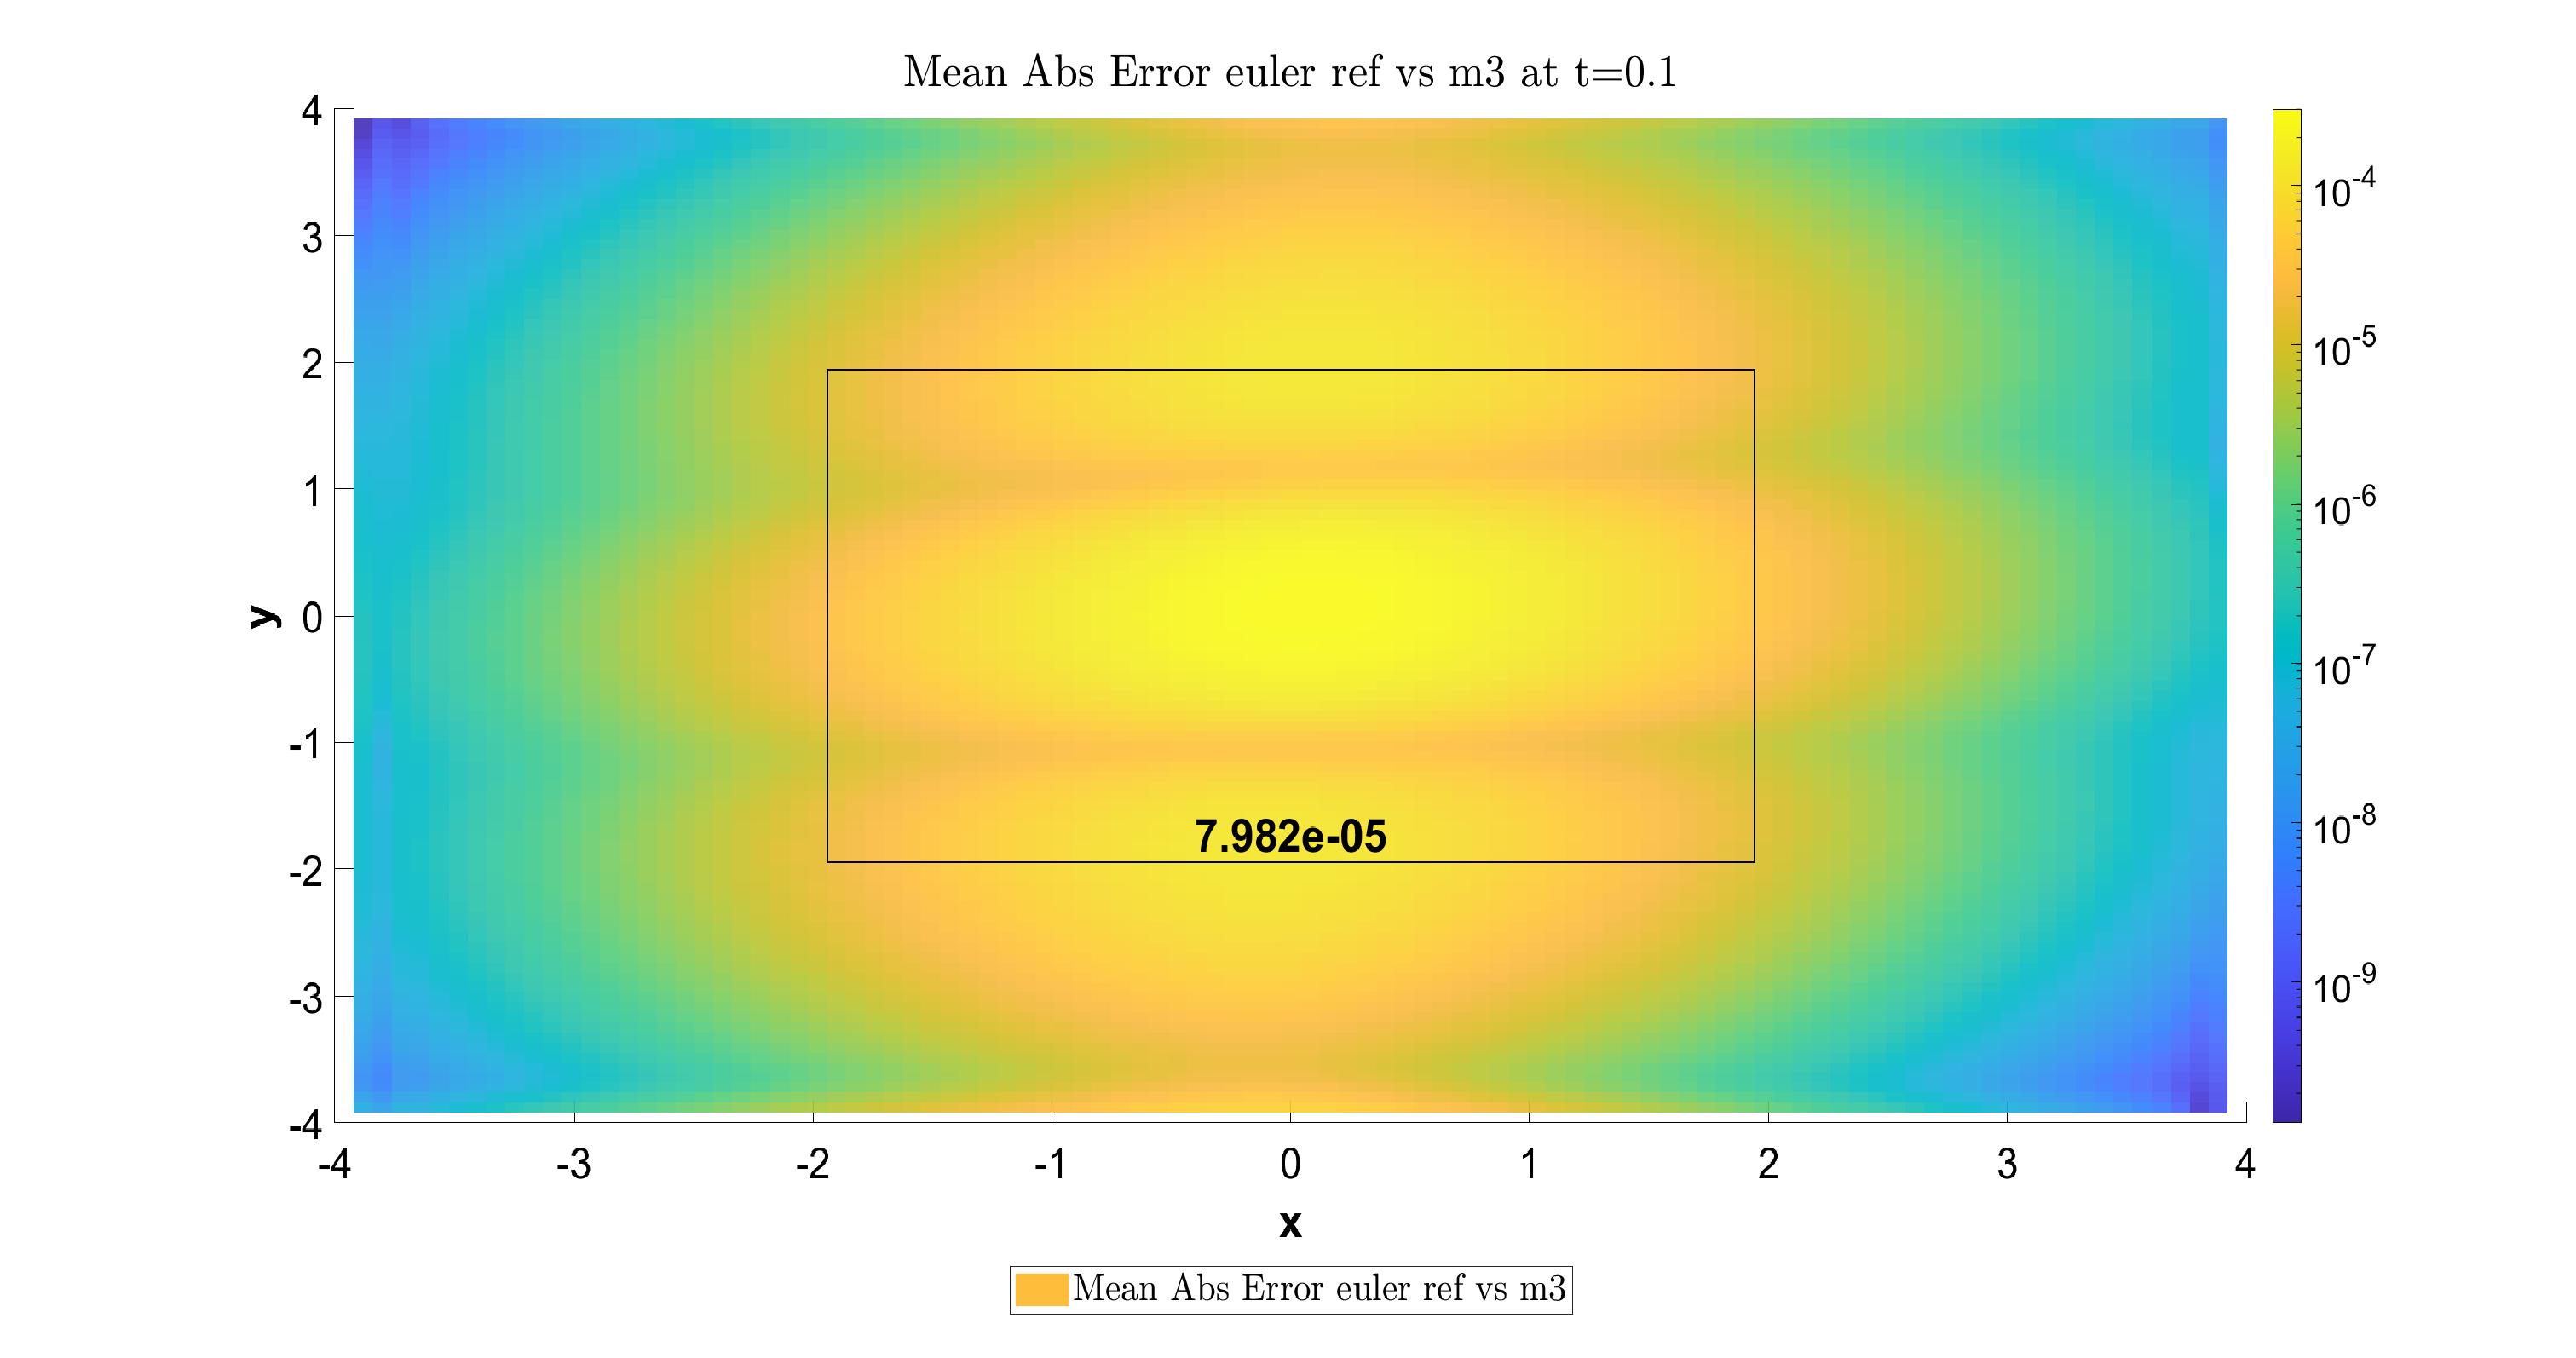
\includegraphics[width=.95\columnwidth]{CDF/CDFEulerRef_9}
\end{landscape}
\begin{landscape}
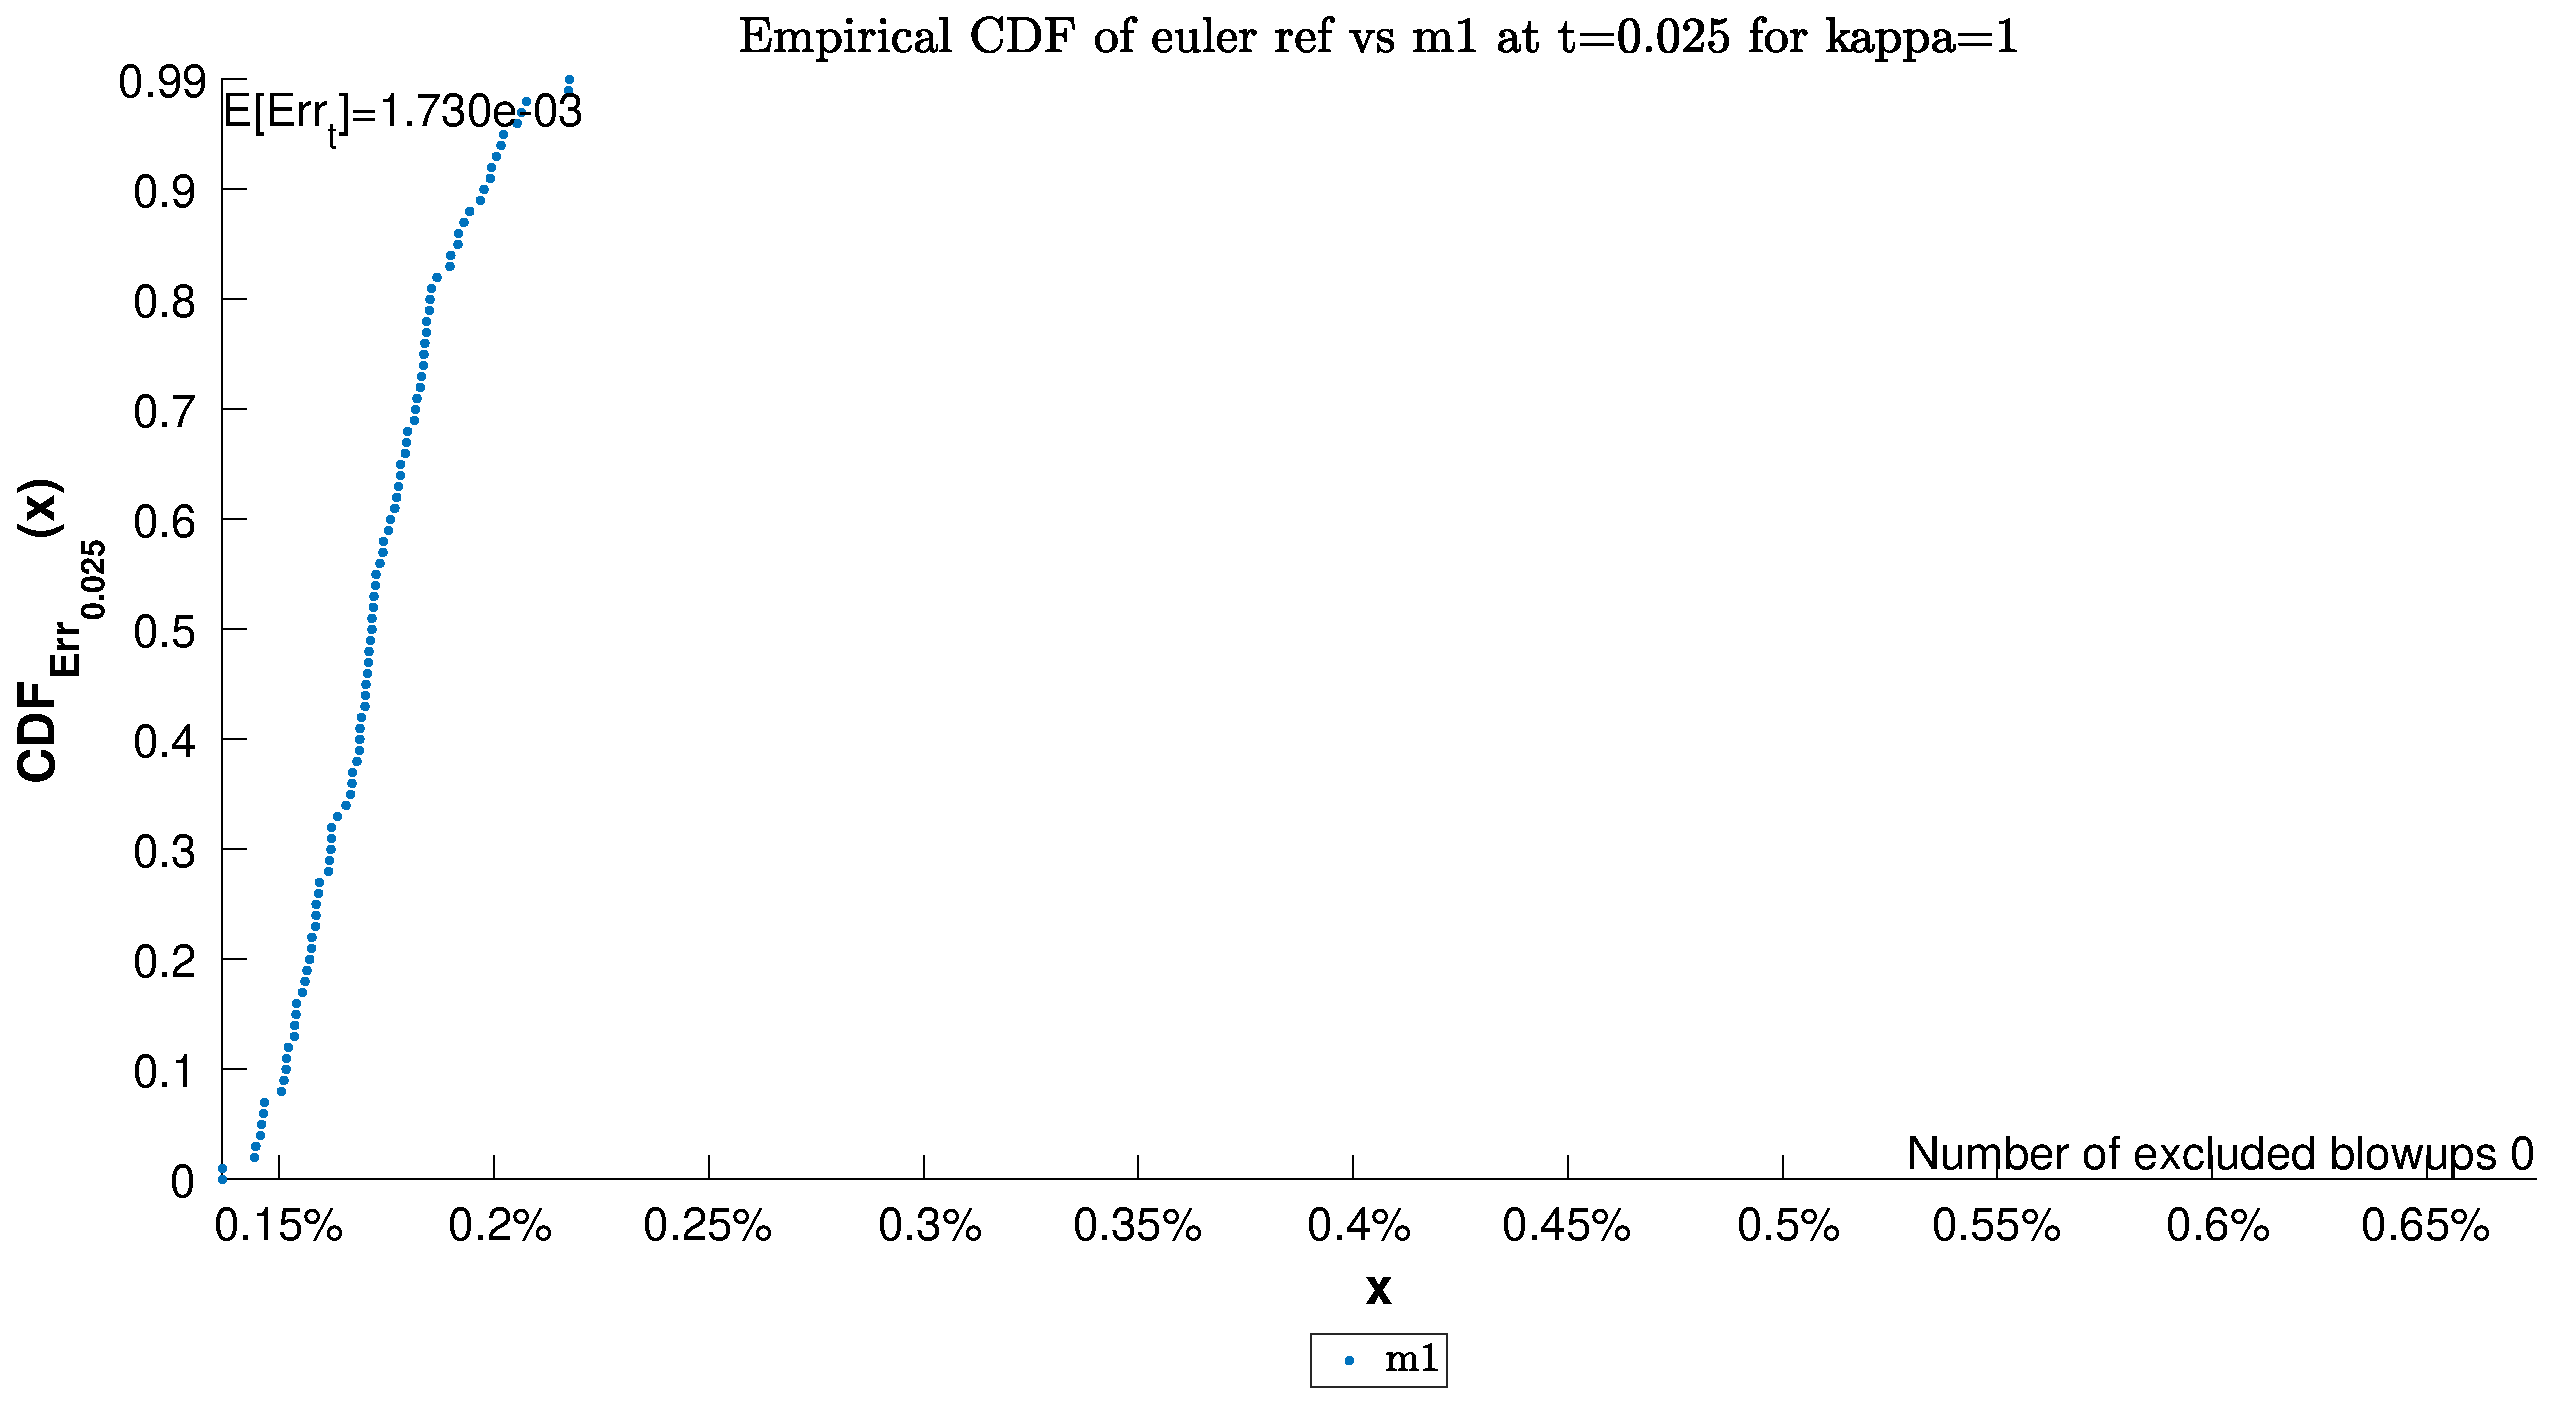
\includegraphics[width=.95\columnwidth]{CDF/CDFEulerRef_10}
\end{landscape}
\begin{landscape}
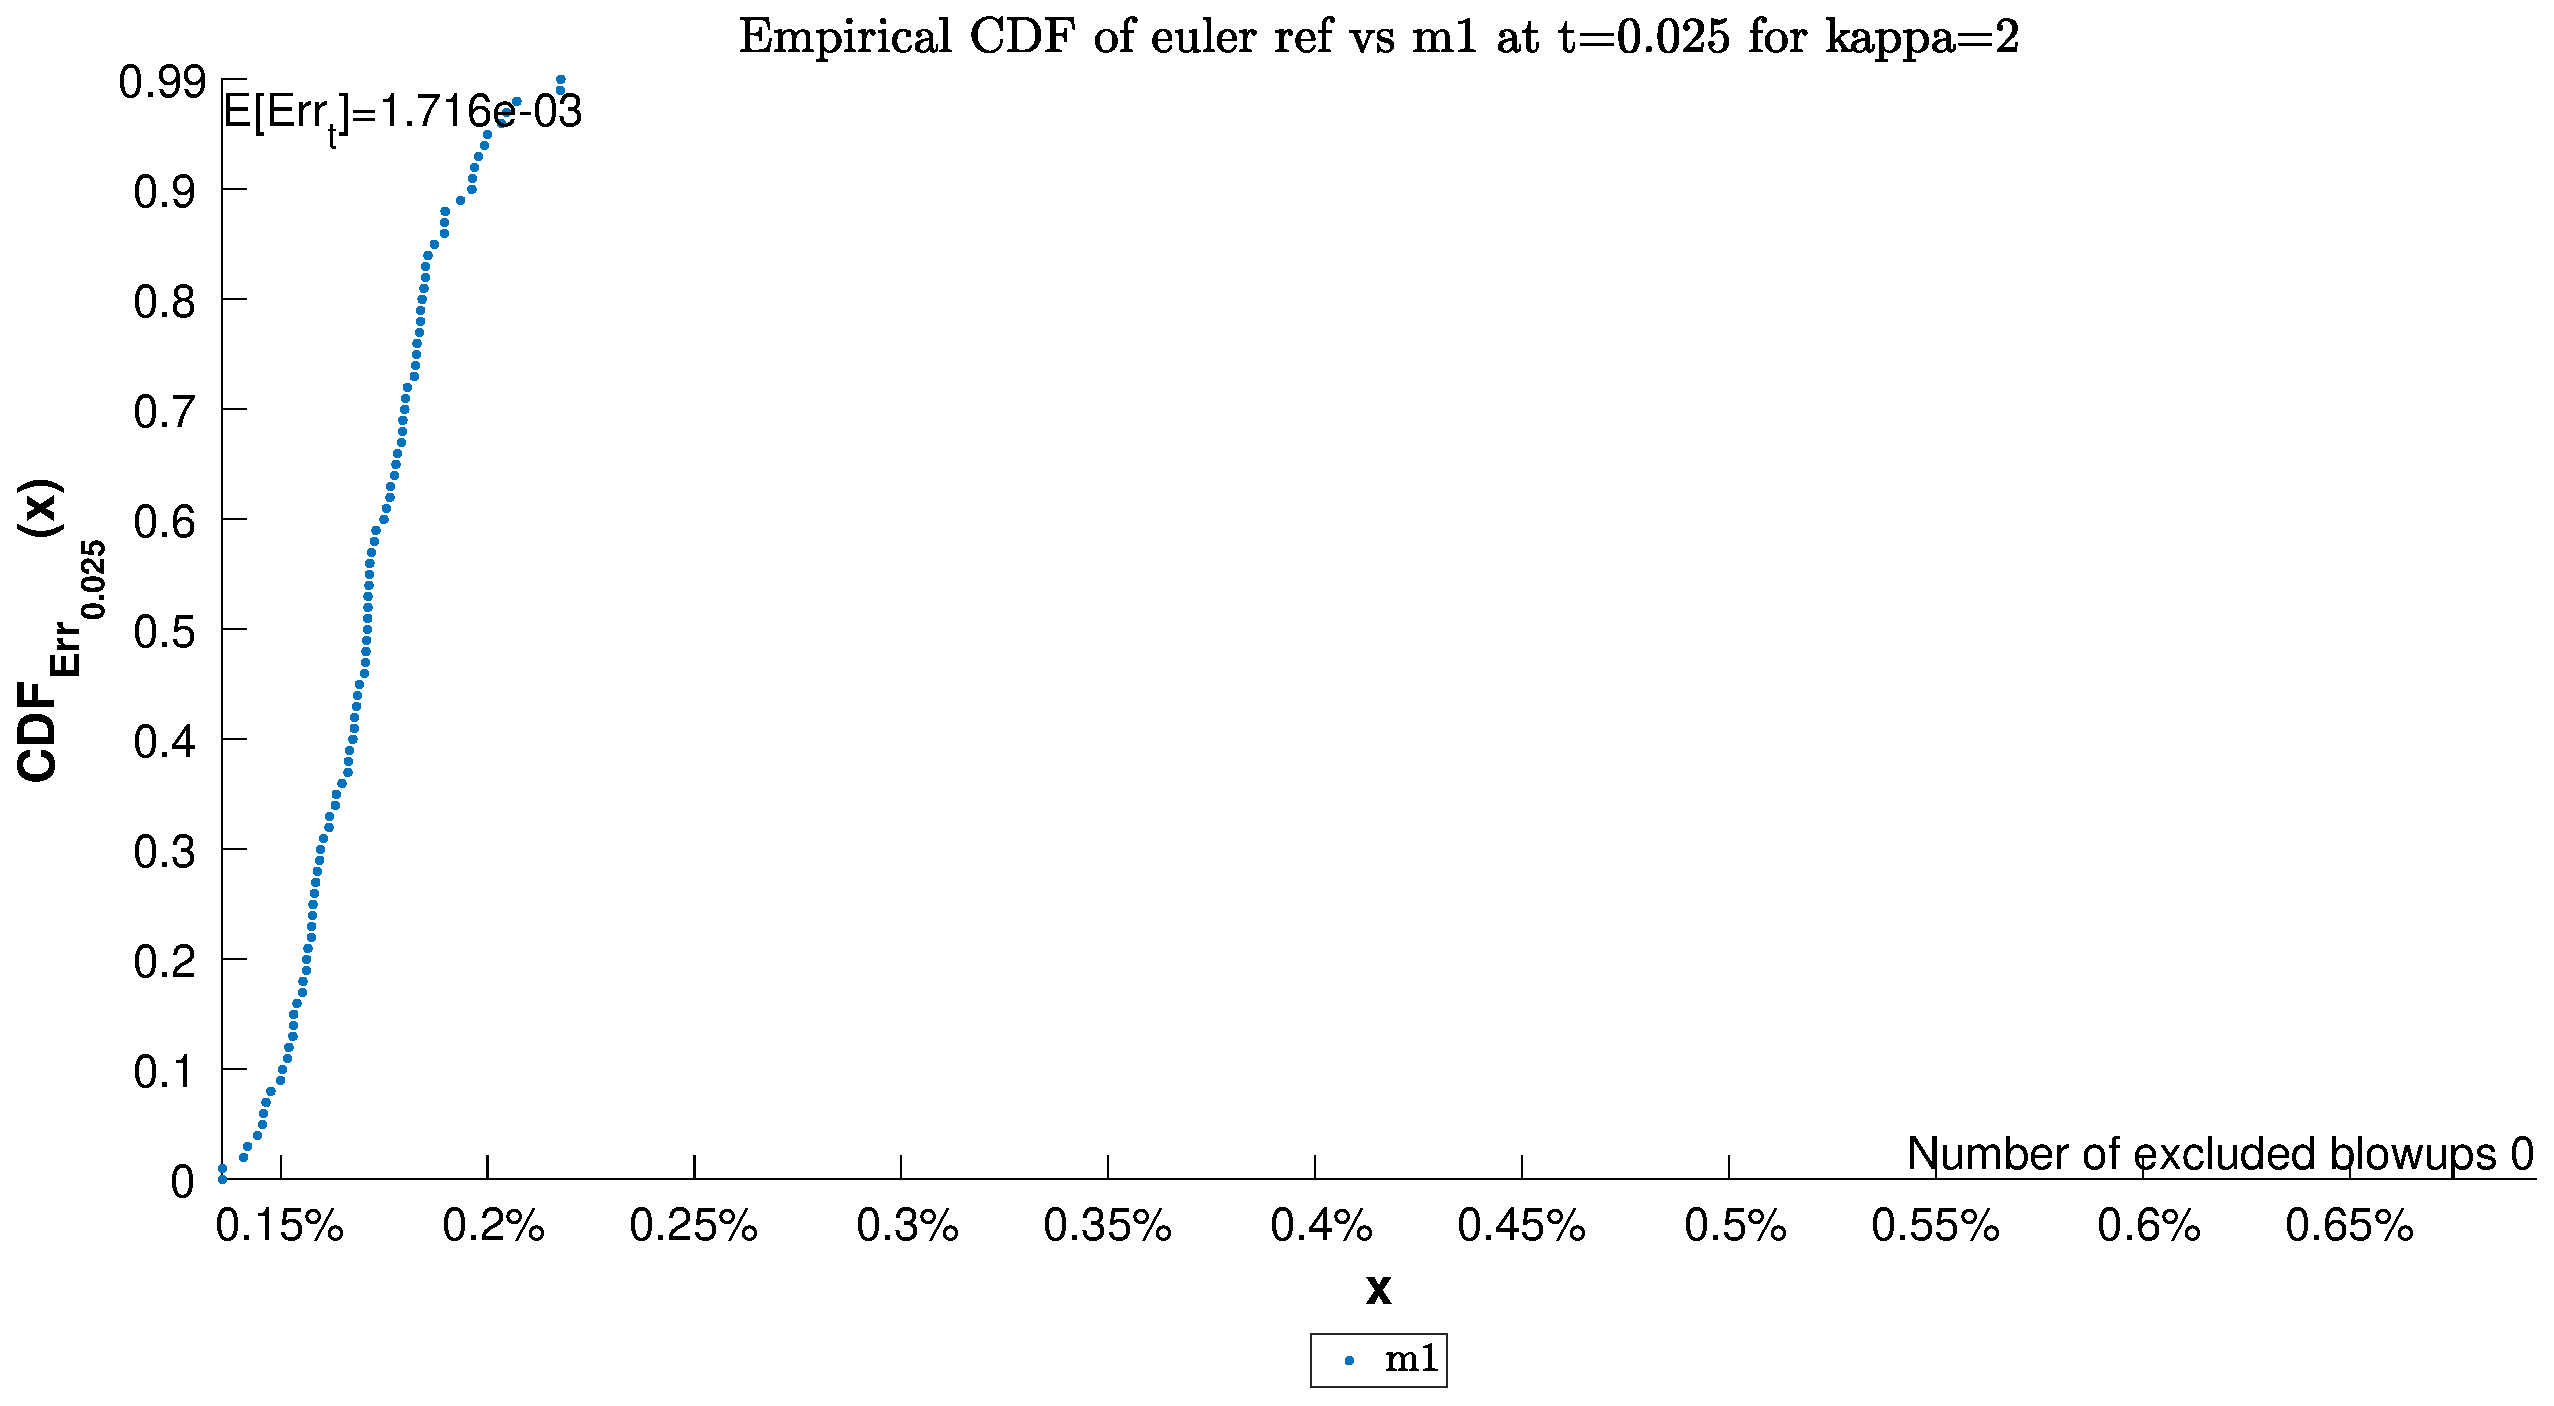
\includegraphics[width=.95\columnwidth]{CDF/CDFEulerRef_11}
\end{landscape}
\begin{landscape}
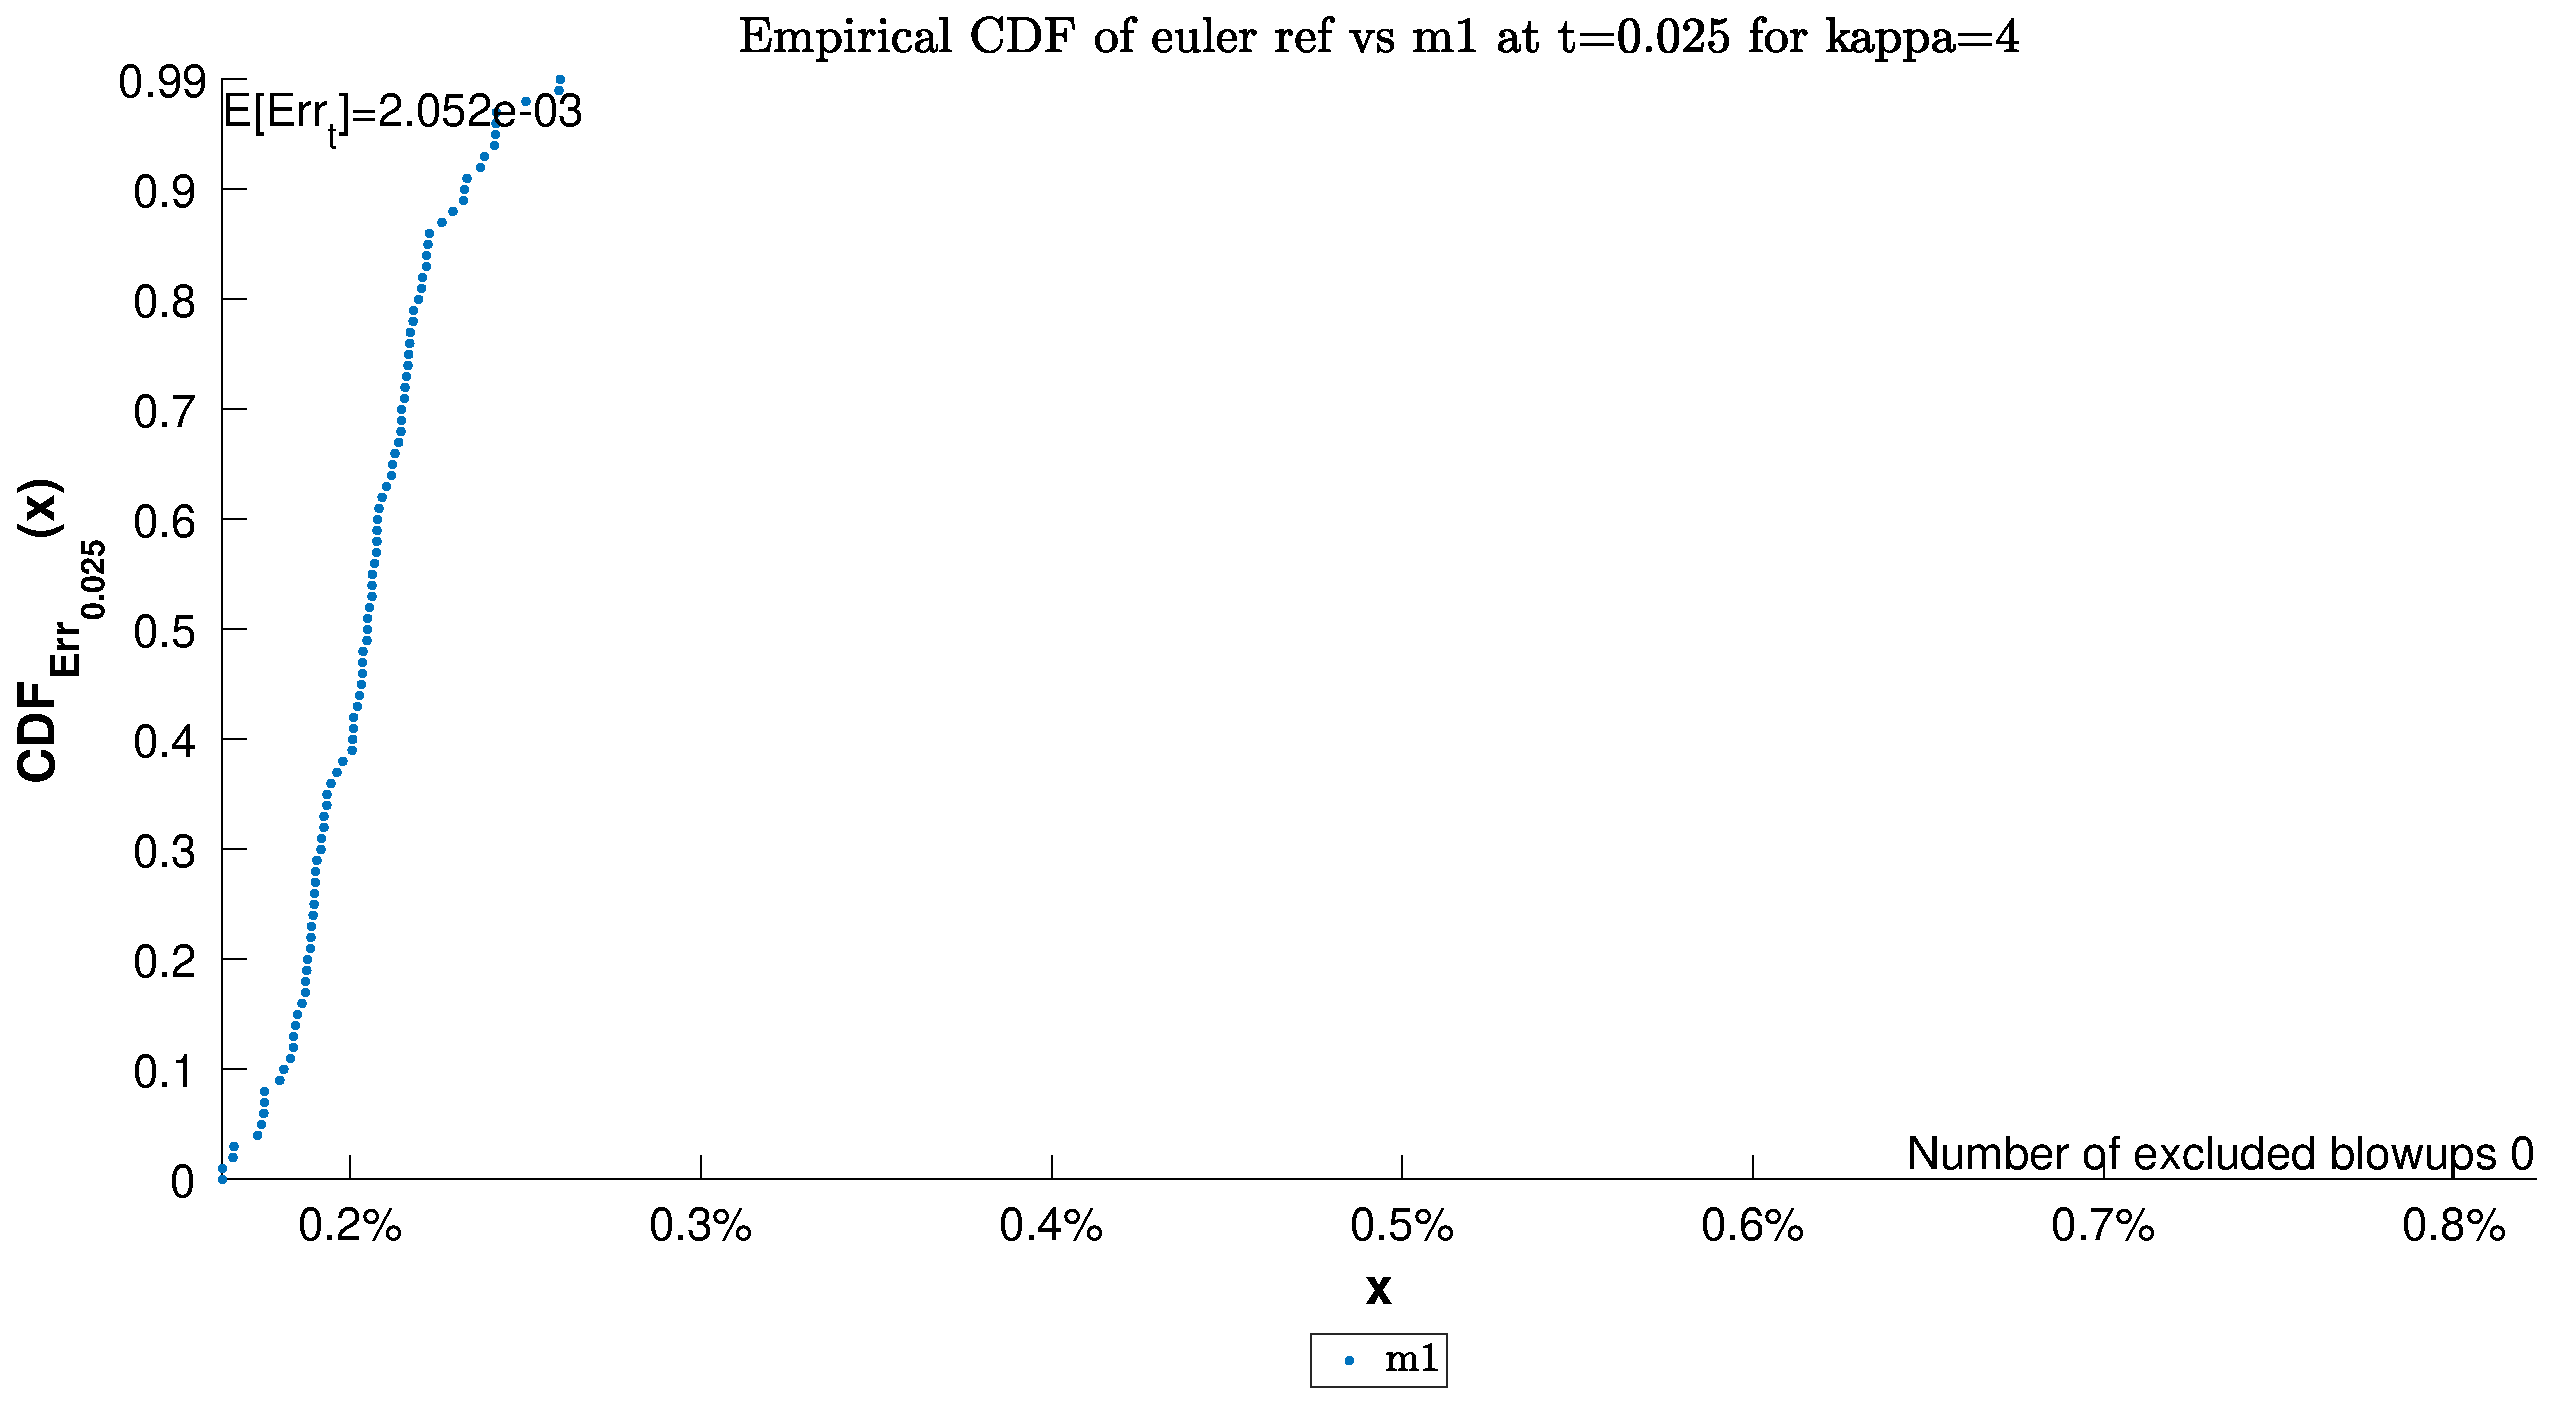
\includegraphics[width=.95\columnwidth]{CDF/CDFEulerRef_12}
\end{landscape}
\begin{landscape}
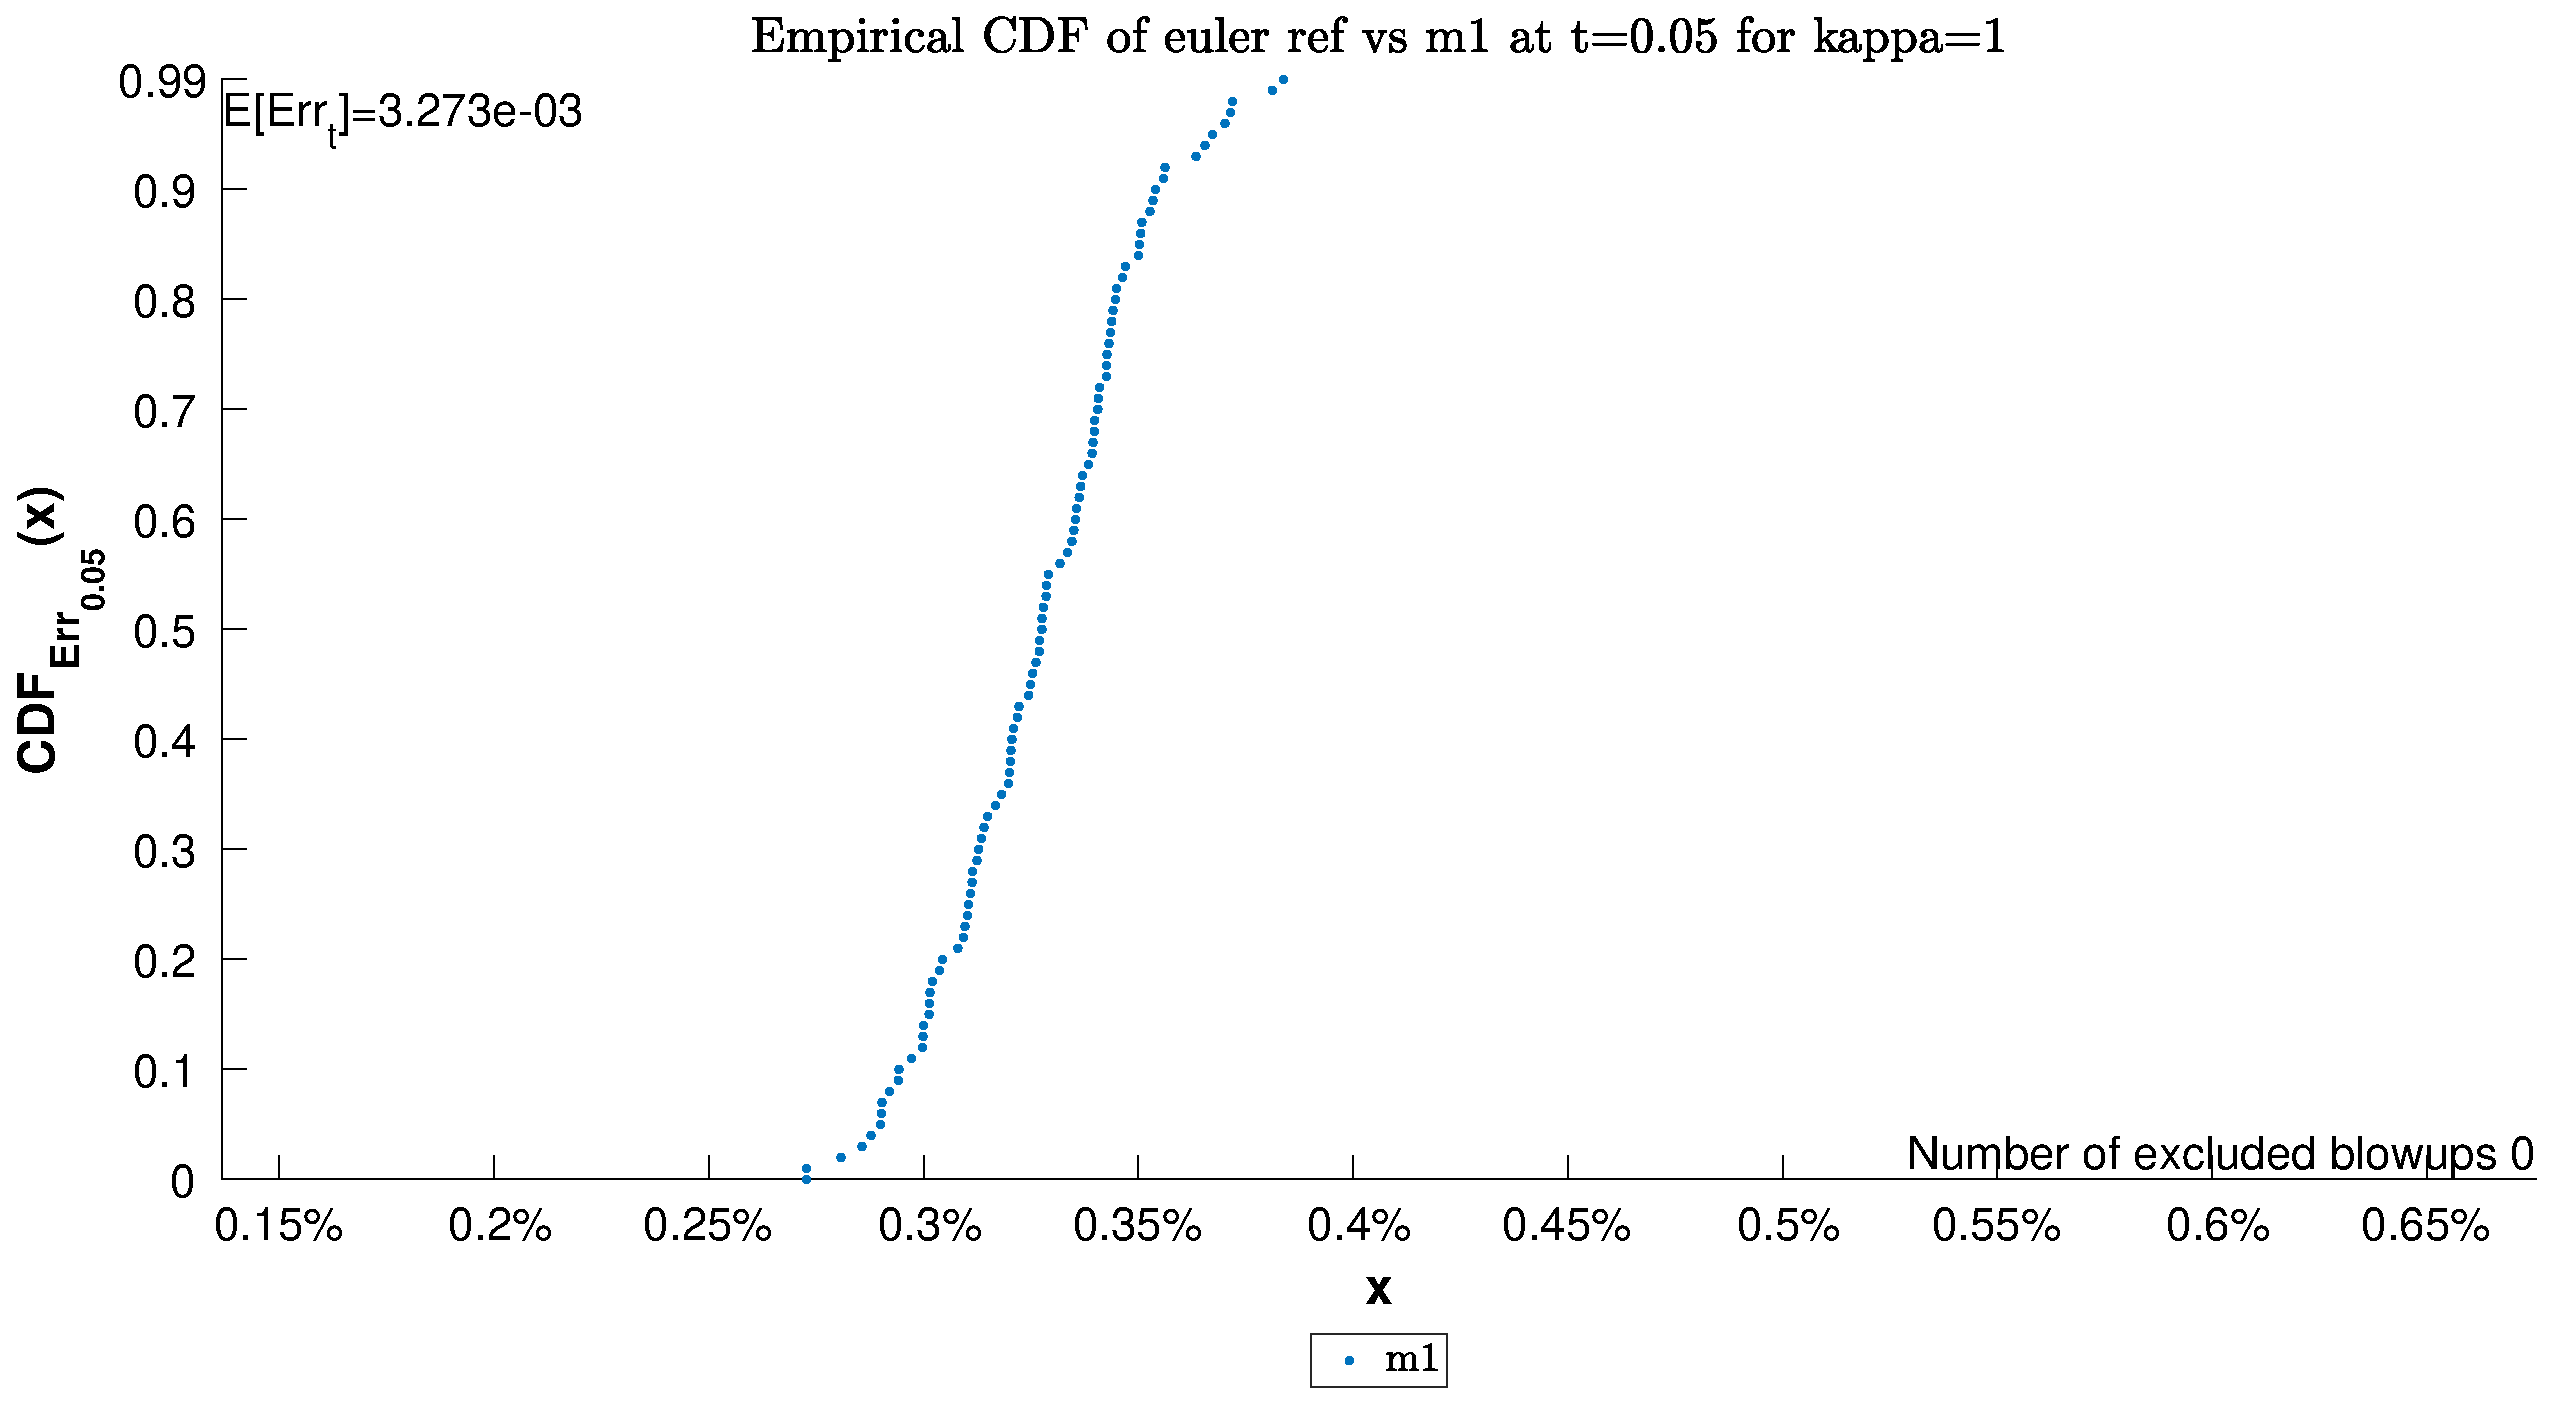
\includegraphics[width=.95\columnwidth]{CDF/CDFEulerRef_13}
\end{landscape}
\begin{landscape}
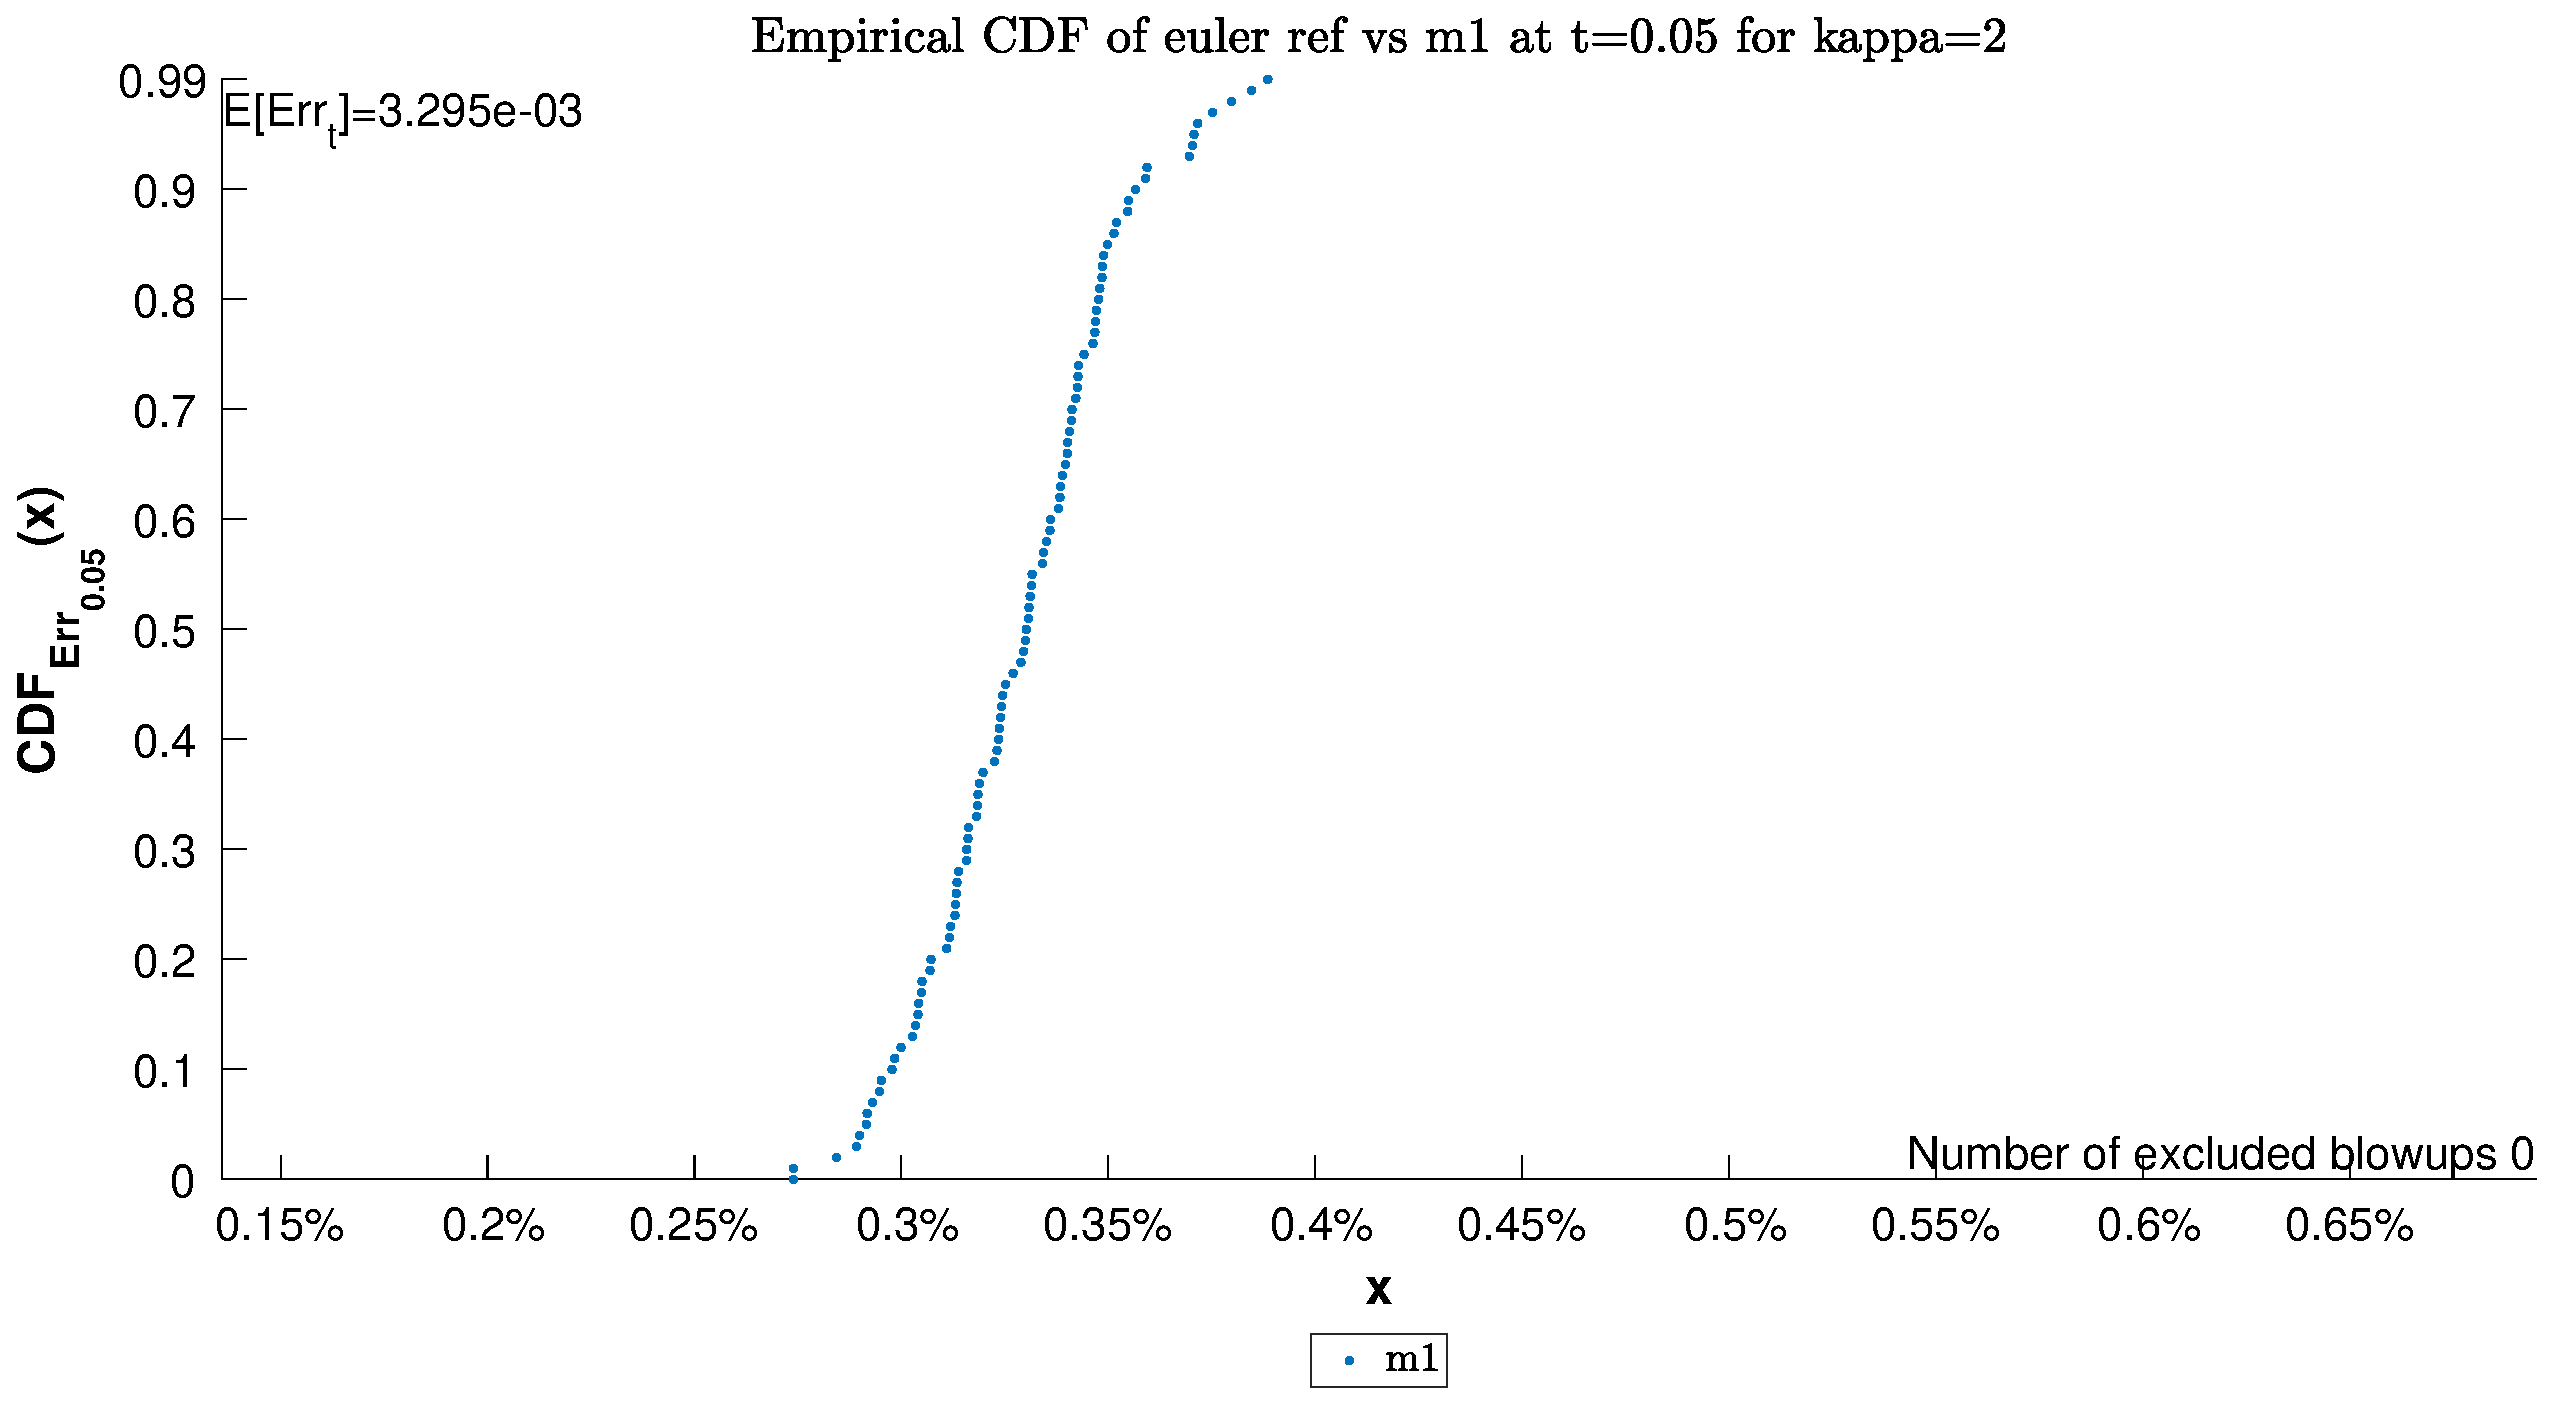
\includegraphics[width=.95\columnwidth]{CDF/CDFEulerRef_14}
\end{landscape}
\begin{landscape}
\includegraphics[width=.95\columnwidth]{CDF/CDFEulerRef_15}
\end{landscape}
\begin{landscape}
\includegraphics[width=.95\columnwidth]{CDF/CDFEulerRef_16}
\end{landscape}
\begin{landscape}
\includegraphics[width=.95\columnwidth]{CDF/CDFEulerRef_17}
\end{landscape}
\begin{landscape}
\includegraphics[width=.95\columnwidth]{CDF/CDFEulerRef_18}
\end{landscape}
\begin{landscape}
\includegraphics[width=.95\columnwidth]{CDF/CDFEulerRef_19}
\end{landscape}
\begin{landscape}
\includegraphics[width=.95\columnwidth]{CDF/CDFEulerRef_20}
\end{landscape}
\begin{landscape}
\includegraphics[width=.95\columnwidth]{CDF/CDFEulerRef_21}
\end{landscape}
\begin{landscape}
\includegraphics[width=.95\columnwidth]{CDF/CDFEulerRef_22}
\end{landscape}
\begin{landscape}
\includegraphics[width=.95\columnwidth]{CDF/CDFEulerRef_23}
\end{landscape}
\begin{landscape}
\includegraphics[width=.95\columnwidth]{CDF/CDFEulerRef_24}
\end{landscape}
\begin{landscape}
\includegraphics[width=.95\columnwidth]{CDF/CDFEulerRef_25}
\end{landscape}
\begin{landscape}
\includegraphics[width=.95\columnwidth]{CDF/CDFEulerRef_26}
\end{landscape}
\begin{landscape}
\includegraphics[width=.95\columnwidth]{CDF/CDFEulerRef_27}
\end{landscape}
\begin{landscape}
\includegraphics[width=.95\columnwidth]{CDF/CDFEulerRef_28}
\end{landscape}
\begin{landscape}
\includegraphics[width=.95\columnwidth]{CDF/CDFEulerRef_29}
\end{landscape}
\begin{landscape}
\includegraphics[width=.95\columnwidth]{CDF/CDFEulerRef_30}
\end{landscape}
\begin{landscape}
\includegraphics[width=.95\columnwidth]{CDF/CDFEulerRef_31}
\end{landscape}
\begin{landscape}
\includegraphics[width=.95\columnwidth]{CDF/CDFEulerRef_32}
\end{landscape}
\begin{landscape}
\includegraphics[width=.95\columnwidth]{CDF/CDFEulerRef_33}
\end{landscape}
\begin{landscape}
\includegraphics[width=.95\columnwidth]{CDF/CDFEulerRef_34}
\end{landscape}
\begin{landscape}
\includegraphics[width=.95\columnwidth]{CDF/CDFEulerRef_35}
\end{landscape}
\begin{landscape}
\includegraphics[width=.95\columnwidth]{CDF/CDFEulerRef_36}
\end{landscape}


%\subsubsection*{Parameters}
	%%\begin{table}%
		%\input{Pdf/temp/param.tex}
		%%\caption{}
		%%\label{}
	%%\end{table}
%\subsubsection*{Errors}
	%%\begin{table}%
		%\input{Pdf/temp/errors.tex}
		%%\caption{}
		%%\label{}
	%%\end{table}
%\subsubsection*{Computational times}
	%%\begin{table}%
		%\input{Pdf/temp/ctimes.tex}
		%%\caption{}
		%%\label{}
	%%\end{table}
%\subsubsection*{Figures}
		%\input{Pdf/temp/figures.tex}
%%\begin{landscape}
	%%%\begin{figure}%
	%%\includegraphics[width=.95\columnwidth]{Pdf/temp/figures.png}%
	%%%\caption{}%
	%%%\label{}%
	%%%\end{figure}
%%\end{landscape}
\end{document}